%%%%%%%%%%%%%%%%%%%%%%%%%%%%%%%%%%%%%%%%%%%%%%%%%%%%
%%%     Language Science Press Master File       %%%
%%%%%%%%%%%%%%%%%%%%%%%%%%%%%%%%%%%%%%%%%%%%%%%%%%%%

\documentclass[output=book,
               leqno,
               booklanguage=english,
               chinesefont
%                draftmode,
%                colorlinks,
%                citecolor=orange
              ]{langscibook}  
%%%%%%%%%%%%%%%%%%%%%%%%%%%%%%%%%%%%%%%%%%%%%%%%%%%%
%%%          additional packages                 %%%
%%%%%%%%%%%%%%%%%%%%%%%%%%%%%%%%%%%%%%%%%%%%%%%%%%%%
\author{Hossep Dolatian}
\title{Adjarian's {\itshape Armenian dialectology} (1911)}
\subtitle{Translation and commentary}

\renewcommand{\lsSeriesNumber}{4}
\renewcommand{\lsSeries}{loc}

\BackBody{Armenian is an Indo-European language that boasts a rich linguistic landscape comprising Classical Armenian (CA), Standard Western Armenian (SWA or WA), Standard Eastern Armenian (SEA or EA), and numerous non-standard dialects, many of which were tragically lost due to the Armenian Genocide. This book is an English translation and commentary of Hratchia Adjarian's seminal work \armenian{Հայ բարբառագիտութիւն} \textit{Armenian dialectology}, originally written in Armenian in 1911. Adjarian describes 31 non-standard Armenian varieties, offering insights into their linguistic structures and historical roots. To enhance accessibility and understanding, this translation unpacks implicit knowledge embedded in Adjarian's text, providing morpheme segmentation, glossing, and translations. This translation is tailored for three distinct audiences: linguists of non-Armenian, traditional Armenian dialectologists, and linguists of Armenian who were trained outside Armenia. This translation aims to bridge linguistic methodologies and facilitate deeper comprehension of Armenian dialectology. The translator supplements Adjarian's prose with commentary, ensuring clarity and accessibility across diverse readerships. This translation provides access to a linguistic landscape of Armenian before the genocide, with the hope of fostering broader scholarly engagement on Armenian dialects.}

\renewcommand{\lsID}{385}
\renewcommand{\lsISBNdigital}{978-3-96110-489-5}
\renewcommand{\lsISBNhardcover}{978-3-98554-118-8}
\BookDOI{10.5281/zenodo.14008766}
\typesetter{Sebastian Nordhoff}
\proofreader{Yasna}

% add all extra packages you need to load to this file

\usepackage{tabularx,multicol}
\usepackage{url}
\urlstyle{same}

\usepackage{listings}
\lstset{basicstyle=\ttfamily,tabsize=2,breaklines=true}

\usepackage{langsci-basic}
\usepackage{langsci-optional}
\usepackage{langsci-lgr}
\usepackage{langsci-osl}
% \usepackage{./langsci/styles/langsci-lgr}
% \usepackage{./langsci/styles/langsci-osl}
% \usepackage{langsci-gb4e}

\usepackage{tikz}
\usetikzlibrary{patterns,calc}
\pgfdeclarepatternformonly{south east lines}{\pgfqpoint{-0pt}{-0pt}}{\pgfqpoint{3pt}{3pt}}{\pgfqpoint{3pt}{3pt}}{
    \pgfsetlinewidth{0.6pt}
    \pgfpathmoveto{\pgfqpoint{0pt}{3pt}}
    \pgfpathlineto{\pgfqpoint{3pt}{0pt}}
    \pgfpathmoveto{\pgfqpoint{.2pt}{-.2pt}}
    \pgfpathlineto{\pgfqpoint{-.2pt}{.2pt}}
    \pgfpathmoveto{\pgfqpoint{3.2pt}{2.8pt}}
    \pgfpathlineto{\pgfqpoint{2.8pt}{3.2pt}}
    \pgfusepath{stroke}}
    
\usepackage{stmaryrd}
\usepackage{wasysym}
\usepackage{multirow}
\usepackage{caption}
\usepackage{subcaption}
\usepackage{mathrsfs}
\usepackage{qtree}

\usepackage{linguex}


%% hyphenation points for line breaks
%% Normally, automatic hyphenation in LaTeX is very good
%% If a word is mis-hyphenated, add it to this file
%%
%% add information to TeX file before \begin{document} with:
%% %% hyphenation points for line breaks
%% Normally, automatic hyphenation in LaTeX is very good
%% If a word is mis-hyphenated, add it to this file
%%
%% add information to TeX file before \begin{document} with:
%% %% hyphenation points for line breaks
%% Normally, automatic hyphenation in LaTeX is very good
%% If a word is mis-hyphenated, add it to this file
%%
%% add information to TeX file before \begin{document} with:
%% \include{localhyphenation}
\hyphenation{
    Beck-man
    Ngu-yen
    back-chan-nel
    back-chan-nels
    mo-not-o-nous
    ste-reo-typ-i-cal
}

\hyphenation{
    Beck-man
    Ngu-yen
    back-chan-nel
    back-chan-nels
    mo-not-o-nous
    ste-reo-typ-i-cal
}

\hyphenation{
    Beck-man
    Ngu-yen
    back-chan-nel
    back-chan-nels
    mo-not-o-nous
    ste-reo-typ-i-cal
}

\addbibresource{localbibliography.bib}

\makeindex[title=Author index] % added March 2024
\makeindex[name=sbj,title=Subject index] % added March 2024


%\includeonly{chapters/call}

%%%%%%%%%%%%%%%%%%%%%%%%%%%%%%%%%%%%%%%%%%%%%%%%%%%%
%%%             Frontmatter                      %%%
%%%%%%%%%%%%%%%%%%%%%%%%%%%%%%%%%%%%%%%%%%%%%%%%%%%%
\WarningFilter{latexfont}{Font shape `T}
% \includeonly{chapters/call,chapters/text-and-speech}
\begin{document}
%pminos do not split footnotes
% \interfootnotelinepenalty=10000 %Footnote in Laporte chapters has to be split SN


%\DeclareIndexNameFormat{default}{%
%\nameparts{#1}%
%\usebibmacro{index:name}%
%{\index[names]}%
%{\namepartfamily}%
%{\namepartgiveni}%
% {}% L1
% {}% L2
%{\namepartprefix}% generates spurious space L3
%{\namepartsuffix}% generates spurious space L4
%}

%  {\DeclareIndexNameFormat{default}{%
%     \usebibmacro{index:name}{\index[names]}{#1}{#3}{#5}{#7}}}

%\DeclareIndexNameFormat{default}{%
%  \usebibmacro{index:name}{\sindex[nom]}{#1}{#3}{#5}{#7}}

%\DeclareIndexNameFormat{default}{%
%  \usebibmacro{index:name}{\sindex[person]}{#1}{#3}{#5}{#7}}
%\DeclareIndexNameFormat{default}{%
%\nameparts{#1} \usebibmacro{index:name}{\sindex[person]]}{\namepartfamily}{‌​\namepartgiven}{\nam‌​epartprefix}{\namepa‌​rtsuffix}}

%\newcommand{\smiley}{:)}

%\renewbibmacro*{index:name}[5]{%
%\usebibmacro{index:entry}{#1}%
%{\iffieldundef{usera}{}{\thefield{usera}\actualoperator}\mkbibindexname{#2}{#3}{#4}{#5}}}

% \newcommand{\noop}[1]{}

%remove for final
%\overfullrule=1mm

\newcommand{\tobi}[2]}}
\renewcommand{\S}[1]{\tobi{#1}{\textsc{*}}}

% this volume references
% puts: [this volume]
% already defined: \citetv
%\newcommand{\citepv}[1]{(\citeauthor{#1} \citeyear*{#1} [this volume])}
\newcommand{\citealtv}[1]{\citeauthor{#1} \citeyear*{#1} [this volume]}

%parentheses around example number
\newcommand{\pref}[1]{(\ref{#1})}

% in-text examples

\newcommand{\lnex}[1]{\textit{#1}} %target lang word
\newcommand{\lnlit}[1]{(lit.: `#1')} %literal reading
\newcommand{\lnlat}[1]{(#1)} % latinization
\newcommand{\lntrans}[1]{`#1'} %translation
\newcommand{\lnexl}[2]%
{\lnex{#1}{} \lnlat{#2}} % ex with latinization
\newcommand{\lnexlat}[3]{\lnex{#1}{} \lnlat{#2}{} \lntrans{#3}} % ex with latinization and tranl.

%ch01
\newcommand{\co}[1]{\mbox{\textbf{#1}}}

%ch09

\newcommand{\cyrbulg}[1]{\begin{otherlanguage*}{bulgarian}#1\end{otherlanguage*}}


%ch10
\newcommand{\nlp}{{\small NLP}}
\newcommand{\mwe}{{\small MWE}}
\newcommand{\rae}{{\small RAE}}
\newcommand{\lvc}{{\small LVC}}
\newcommand{\pos}{{\small P}o{\small S}}
%\newcommand{\todo}[1]{ \textcolor{red}{#1} }

%\renewcommand{\labelenumi}{\theenumi}
%\ainamefmt{{vv}{ll}{, ff}{, jj}} % fullname

\newcommand{\biberror}[1]{{\color{red}#1}}

\newcommand{\osenovaitem}{--~}
\maketitle
\frontmatter
\currentpdfbookmark{Contents}{name} % adds a PDF bookmark
{\sloppy\tableofcontents}
%% remove the % in the following lines if your book has these elements
%  \addchap{Preface}

This book has had a rather long gestation period. The papers in this collective volume originate in
a selection of the papers that were presented at a workshop at Freie Universität Berlin in May
2017, which was jointly organised by Ulrike Freywald, then University of Potsdam, and Horst Simon,
FU Berlin. In an elaborate and anonymous peer review process, the papers were selected and revised
under the guidance of UF and HS, and finally refined and brought into their present shape by Stefan
Müller, who had also presented at the workshop, and his team at HU Berlin. 

We thank various institutions and individuals, above all the Deutsche Forschungsgemeinschaft and the
Ernst-Reuter-Gesellschaft der Freunde, Förderer und Ehemaligen der Freien Universität Berlin
e.V. for their financial support of the workshop, then a host of colleagues, who need to remain
anonymous, who have offered their expertise when peer reviewing, and finally a group of student
assistants in the final process of polishing the papers into publishable form, namely Elisabeth
Eberle, Luisa Kalvelage, and Julie Täge.

It is to be hoped that the present volume will testify more to the potential headlessness of the
structures discussed than to the headlessness of the pondering linguist. 

\bigskip
\noindent
Berlin \& Dortmund, \today \hfill \begin{tabular}[t]{@{}r@{}}
                                  Ulrike Freywald\\
                                  Horst J.\ Simon \\
                                  Stefan Müller
                                  \end{tabular}








%%%%%%%%%%%%%%%%%%%%%%%%%%%%%%%%%%%%%%%%%%%%%%%%%%%%
%%%             Chapters                         %%%
%%%%%%%%%%%%%%%%%%%%%%%%%%%%%%%%%%%%%%%%%%%%%%%%%%%%


\setcounter{secnumdepth}{-2}% default for "report" is 2
% in order to include acknowledgements and preface in the Table of Contents without giving them chapter numbes.

\addchap{\lsAcknowledgementTitle} 

\textit{Núu'etaa numá'kaaki wáakapusmak wakápusa wakų́'ro'sh}. 

This book would not have been possible without the generosity and foresight of various Mandan speakers who gave their time and energy into recording their language and their knowledge. Some of the key Mandan individuals who have provided to this corpus, which extends back over a century and a half, include: Mrs. James Kipp (a.k.a., Earth Woman), Mrs. Holding Eagle (a.k.a., Scatter Corn), Mr. Ben Benson (a.k.a., Buffalo Bull Head), Mr. Flat Bear (a.k.a., Bear on the Flat), Mr. Walter Face (a.k.a., Wounded Face), Mrs. Little Crow (a.k.a., Otter Woman), Mr. Paul Crows Heart (a.k.a., Crows Heart), Mr. Sitting Rabbit, Mr. Little Crow, Mr. Wolfs Head, Mr. Wolf Ghost, Mr. White Calf, Mr. Foolish Woman, Mr. Little Owl, Mrs. Good Bear, Mrs. Calf Woman, Mrs. Owen Baker, Mrs. Front Woman, Mr. Wolf Chief, Mrs. White Duck, Mrs. Edna Face, Mrs. Nora Baker, Mr. Stephen Bird, Mr. Mark Mato, Mrs. Bessie Medicine Stone, Mrs. Mary Atkins, Mrs. Blanche Benson, Mr. Burr Crows Breast, Mrs. Annie Eagle, Mrs. Mattie Grinnell, Mr. Albert Little Owl, Mr. Ralph Little Owl, Mrs. Otter Sage, Mr. John Stone, Mr. Clyde Baker, Mr. Jacob, Bird, Mr. William Bell, Mrs. Louella Benson Young Bear, Mr. Ernest Medicine Stone, Mr. Carl Whitman, Ms. Ann Solano, Mr. Leon Little Owl, Mr. Corey Spotted Bear, and Mr. Edwin Benson.

I also gratefully acknowledge that I was able to assemble the materials and information found in this book over the years thanks to the generous financial support of the American Philosophical Society's Phillips Fund for Native American Research, Yale University's A. Richard Diebold Jr. Graduate Fellowship and the Frederick W. Hilles Memorial Scholarship Fellowship, Northeastern Illinois University's Dr. Bernard J. Brommel Doctoral Scholarship, and freelance employment by the Language Conservancy through its contract with the Mandan-Hidatsa-Arikara Nation's Department of Education. I also could never have completed this book without the support provided to me by my employer, the University of Oklahoma, where I had been afforded a semester of teaching release after my third year to ensure that this book could be completed.

My long-time advisor at Yale, Prof. Stephen Anderson, saw many early versions of papers and projects that led to what is now this book. His guidance was instrumental to the theoretical conclusions I made in my dissertation, and that dissertation formed the backbone of the present monograph. Prof. Claire Bowern, my other dissertation co-chair and professor was likewise key to my ability to complete my dissertation, especially after I left New Haven and worked on my dissertation \textit{in absentia} for several years. She held me accountable to making progress, and I deeply appreciate the time and energy she spent in getting me across the finish line. Prof. Natalie Weber, a dissertation committee member, looked over many versions of the analyses that became the chapter on Mandan phonetics and phonology in this book. I am grateful for their time in walking me through more effective ways of presenting the data there. Prof. Marianne Mithun, as a member of my dissertation committee, provided valuable insight into how different processes in Mandan worked and how they fit into the typology of North American languages. Her own experience in studying Siouan languages and her breadth of knowledge on language change improved how I presented the morphological data in what has become the verbal morphology chapter of this book.

On a more personal level, my parents Raymond and Kathleen Kasak have contributed to much to the evolution of this book by asking me repeatedly over the years, ``is it done yet?'' Since the spring of 2015, many phone conversations ended with a question as to the status of this work. First, they asked when I was working on my dissertation, which this book uses as a launchpad for a more comprehensive grammar. Later, as I was preparing this manuscript for submission to Language Science Press, they would ask me whether I was done with this chapter or that chapter yet. Any academic surely understands how incredibly welcome and not at all stressful such questions were.

The friends I made at my M.A in Linguistics at Northeastern Illinois University helped get me to Yale and were, therefore, important to getting this book finished. Dr. John Boyle, first as my professor and then as my friend, introduced me to Siouan linguistics, so I could not have even begun to build the foundations of this book without him. I am thankful for him taking me to my first Siouan and Caddoan Languages Conference in Kansas and him introducing me to the late, great Bob Rankin, one of the monumental figures of Siouan linguistics. My former professors Drs. Shahrzad Mahootian and Lewis Gebhart were great moral support in convincing me to apply to grad school and checked in with me often to see how things were going. My former NEIU classmates Dr. Binh Ngo and Galini Gkartzonika have likewise been great friends and supporters throughout my time at Yale and beyond. I also could not have written this book without the editorial assistance of my wonderful friend Hadley Austin and my former student Lizz Evalen, whose proofreading of an earlier version of my dissertation has made the writing of this book much easier.

My final and most important acknowledgment goes to my partner and wife Dr. Colbi Beam, who has been a singular source of inspiration to complete this work. I am forever grateful for her love and support. I have no doubt that this book would have taken far longer to complete without her encouragement and her understanding of what it takes to write academically. Having written a dissertation herself, she understood the nature of writing expansive pieces of work and she was helpful in putting aspects of the writing process in perspective for me during times when I struggled with how to present some data or was unsure how to best resolve some impasse in writing. She has been insightful and inspirational throughout this process. Colbi, you are simply the best.
\addchap{Preface}

This book has had a rather long gestation period. The papers in this collective volume originate in
a selection of the papers that were presented at a workshop at Freie Universität Berlin in May
2017, which was jointly organised by Ulrike Freywald, then University of Potsdam, and Horst Simon,
FU Berlin. In an elaborate and anonymous peer review process, the papers were selected and revised
under the guidance of UF and HS, and finally refined and brought into their present shape by Stefan
Müller, who had also presented at the workshop, and his team at HU Berlin. 

We thank various institutions and individuals, above all the Deutsche Forschungsgemeinschaft and the
Ernst-Reuter-Gesellschaft der Freunde, Förderer und Ehemaligen der Freien Universität Berlin
e.V. for their financial support of the workshop, then a host of colleagues, who need to remain
anonymous, who have offered their expertise when peer reviewing, and finally a group of student
assistants in the final process of polishing the papers into publishable form, namely Elisabeth
Eberle, Luisa Kalvelage, and Julie Täge.

It is to be hoped that the present volume will testify more to the potential headlessness of the
structures discussed than to the headlessness of the pondering linguist. 

\bigskip
\noindent
Berlin \& Dortmund, \today \hfill \begin{tabular}[t]{@{}r@{}}
                                  Ulrike Freywald\\
                                  Horst J.\ Simon \\
                                  Stefan Müller
                                  \end{tabular}






%  \addchap{\lsAbbreviationsTitle}
% \addchap{Abbreviations and symbols}
The category labels for abbreviations follow the Leipzig Glossing Rules.\footnote{\url{http://www.eva.mpg.de/lingua/resources/glossing-rules.php}}
\vspace{.5cm}

\begin{tabularx}{.45\textwidth}{lQ}
    ∅ & zero form \\
    \textbackslash.../ & verb stem\\
    . & multi-item gloss (3\textsc{sg.m})\\
    \_ & multi-item lexemes (like\_that)\\
    - & for affixes (\textit{-thé})\\
    = & for clitics (\textit{=en})\\
    | & syncretism (2|3 person)\\
    > & argument structure (1>3 `first person acting on third person')\\
    1 & first person\\
    2 & second person\\
    3 & third person\\
    \textsc{abs} & absolutive\\    
    \textsc{absc} & absconditive (attention getter, `look here')\\
	\textsc{adjz} & adjectivizer\\
    \textsc{all} & allative\\
    \textsc{and} & andative (`away')\\
    \textsc{anim} & animate\\
    \textsc{appr} & apprehensive\\
    \textsc{assoc} & associative case\\
    \textsc{char} & characteristic case\\
    \textsc{dat} & dative case\\
    \textsc{dem} & anaphoric demonstrative\\
\end{tabularx}
\begin{tabularx}{.45\textwidth}{lQ}
    \textsc{dia} & diathetic prefix\\
    \textsc{dim} & diminutive\\
    \textsc{dist} & distal deictic\\
    \textsc{distr} & ditributive\\
    \textsc{du} & dual number\\
    \textsc{dur} & durative\\
    \textsc{emph} & emphatic\\
    \textsc{erg} & ergative case\\
    \textsc{etc} & et cetera (`and all')\\
    \textsc{f} & feminine\\
    \textsc{fut} & future\\
    \textsc{futimp} & future imperative\\
    \textsc{iam} & iamitive (`already')\\
    \textsc{ic} & inclusory case\\
    \textsc{imn} & imminent (`about to')\\
    \textsc{imp} & imperative\\
    \textsc{indf} & indefinite\\
    \textsc{ins} & instrumental case\\
    \textsc{io} & indirect object\\
    \textsc{ipfv} & imperfective\\
    \textsc{ipst} & immediate past\\
    \textsc{irr} & irrealis\\
    \textsc{iter} & iterative\\
    \textsc{loc} & locative case\\
    \textsc{lpl} & large plural\\
    \textsc{m} & masculine\\
    \textsc{med} & medial deictic\\
\end{tabularx}
\newpage
\begin{tabularx}{.45\textwidth}{lQ}
    \textsc{nd} & non-dual\\
    \textsc{neg} & negator\\
    \textsc{nmlz} & nominalizer\\
    \textsc{npl} & non-plural\\
	\textsc{npst} & non-past\\
	\textsc{nsg} & non-singular\\
    \textsc{only} & exclusive marker (`only', `just')\\
    \textsc{pfv} & perfective\\
    \textsc{ph} & placeholder (`thingamajig')\\
    \textsc{pl} & plural\\
    \textsc{pn} & proper name\\
    \textsc{pln} & place name\\
    \textsc{poss} & possessive\\
\end{tabularx}
\begin{tabularx}{.45\textwidth}{lQ}
    \textsc{pot} & potential\\
    \textsc{priv} & privative case\\
	\textsc{prop} & proprietive case\\
    \textsc{prox} & proximal deictic\\
    \textsc{pst} & past\\
    \textsc{purp} & purposive case\\
    \textsc{q} & question\\    
    \textsc{quot} & quotative\\
    \textsc{redup} & reduplication\\
	\textsc{rpst} & recent past\\
    \textsc{sg} & singular\\
    \textsc{simil} & similative case\\
    \textsc{stat} & stative\\
    \textsc{temp} & temporal case\\
    \textsc{vent} & venitive (`towards')\\
\end{tabularx}
\mainmatter

% in order to include acknowledgements and preface in the Table of Contents without giving them chapter numbes.

\setcounter{secnumdepth}{2}

\chapter[Encoding language]{Encoding language on computers}
\label{ch:encodings}

\section{What is language?}

This book aims to introduce you to the different ways that computers are able to process natural language.  To start off, then, we can ask: What is language?  You're using language to read this book, so you have some intuitive idea of what it is, but if you've never studied linguistics before, you might not have a clear definition in mind.

In an attempt to distinguish between language and other animal communication systems, the anthropologist  Charles \citet{Hockett:1960}  proposed some properties that together make language special:

\begin{enumerate}
    \item Language is produced vocally and understood with the auditory system, or in the case of signed languages, signed with the body and perceived visually.
    \item Language is produced intentionally. People intend to say what they say.
    \item Language is transitory: Unless you write down what is said, it is ephemeral.  As we will explore in detail later, writing -- crucially \emph{not} transitory -- is distinct from language.
    \item Language is interchangeable: Anything that you can hear, you can also say, and vice versa, regardless of its truth or its relation to you. (In contrast, in the realm of animal communication, queen ants produce a chemical signal that other ants cannot produce, meaning that chemical communication for ants is non-interchangeable.)
    \item Language involves total feedback: Speakers can hear their own speech, and signers can see their own signing.  People know what they are saying.
    \item When people speak or sign, the sounds/signs that they produce are specifically intended for communication, not secondary to any other purpose.  (In contrast, a dog may indirectly convey that it is hot by panting, but the primary purpose of panting is to cool the dog off, not to communicate.)
    \item Specific words/signs are attached to specific meanings.
    \item The relation between sounds/signs and meaning is mostly \keyword{arbitrary}, chosen by convention.  There is no particular reason to call a dog a \exword{dog} except that our community has agreed to it; other communities have chosen other conventions (\exword{perro}, \exword{Hund}, etc.).
    \item Even if different people pronounce or sign the same word differently, these  variable realizations are mapped to discrete categories (distinct sounds, signs, or words) in the mind.
    \item Language can be used to talk about things that are absent, imaginary, or false (in contrast to pointing, for example, which is restricted to entities that are present).
    \item Language can be used to lie.
    \item Language is made of discrete units: Sentences/utterances are made of words; words are made of morphemes (pieces of words such as \exword{un-} or \exword{-ing}); morphemes are made of sounds.
    \item Language is \keyword{productive}: You can use it to say and understand things that have never been said before.
    \item Language is learnable: You can learn a (new) language.
    \item Language is culturally transmitted: You learn the
      language(s) surrounding you.
    \item Language is reflexive: As we're doing here, you can use language to talk about itself.

\end{enumerate}

Using these distinctive features, you should now be able to explain why music, mathematics, and programming languages -- as amazing and useful as they are -- do not constitute language in Hockett's sense, even if they share some elements in common with it.

\section{Language versus writing}

Language is perhaps the most amazing technology that humans have ever created: It allows us to teach and learn,  explain complicated ideas,  build social relationships and societies,  create laws and promises,  ask and answer questions, make and respond to commands, tell stories, imagine alternate realities, understand what other people believe,  recount the past and plan for the future, and  collaborate to get things done.


It is important to understand that language is distinct from writing.  As Hockett notes, spoken/signed utterances are ephemeral; writing constitutes a further amazing technology which represents speech/signing in a system of lasting physical or digital markings.
 Distinguishing language from its written representation,  language is universal across humans: All human societies use language, and every single human child (except for rare cases of extremely severe neglect or disability) learns language without much formal instruction.  In contrast, writing is not universal: Some societies do not use writing.  Indeed, of the seven thousand known spoken languages listed in  \mediatitle{Ethnologue}\footnote{\url{https://ethnologue.com}, accessed 2024-04-19.}, only about sixty percent have writing systems; unwritten languages include the  Gugu Badhun language of Australia, the Southeastern Pomo language of California, and so on. 
Writing generally requires formal instruction, and some people do not learn it even if their society uses it.  Language is also much older than writing; language emerged around 100,000 to 200,000 years ago while writing arose around five or six thousand years ago.  Of course, language is transitory, so its age can only be inferred indirectly, from archaeological artifacts such as decorative beads \citep{BothaKnight:2009}, which indicate a desire to communicate (one's status and appearance) that presumably extends to language. So language is ancient and universal, while writing is new and localized to particular people and societies.

Although it is important to keep language and writing distinct, writing is obviously intimately related to language.  Writing  allows us to do all the things that language allows us to do -- teach, learn, explain, build relationships, organize societies, talk about the past and future, collaborate -- across distances and time.  With writing, you can learn from people you have never met, from past generations and other continents.  You can also keep records of things, such as debts and purchases, that are too complicated to remember; 
%\mad{Do we have a reference or further reading for this? $\to$ Lelia} \faye{Glassner's book "The Invention of Cuneiform" (2003) could be valuable additional reading here?}
indeed, the first Sumerian writing appears to record commercial transactions, involving both language and numeracy  \citep{Glassner:2003}.  Today, thanks to computers and the internet, digital writing allows us to disseminate language instantly around the globe.

The topics explored in this book involve the word \exword{language} -- natural language processing, language technology -- but they largely involve writing, because writing is the primary medium through which computers represent and process language.  We begin our tour by introducing writing systems and their digital representation, then end the chapter by briefly exploring sound.

%Even \keyword{dialog systems} such as Siri and Google Home, which interpret and produce speech, map that speech to text and then to speech again.  Speech/signing is transitory and fades quickly from a listener's memory, whereas writing is sufficiently permanent that it can be manipulated digitally.\wdm{This may come across as a bit simplistic since it \textbf{is} possible to encode spoken language so that it is as permanent as writing. And,  a transcription of speech is not the same as a written text. So should we soften this and reformulate it to be a transition to both writing systems (the next section) and encoding spoken language (coming up in 1.5?) $\to$ Detmar} 





% It's  late 

%As but one example, think about what happens when a friend points at a book and says, \exsent{He's no Shakespeare!}.  First of all, there is the difficulty of determining who is meant by \exsent{he}.  Your friend is pointing at a book, not at a person, and although we can figure out that \exsent{he} most likely refers to the author of the book, this is not obvious to a computer (and sometimes not obvious to the person you are talking with).  Secondly, there is the difficulty of knowing who \exsent{Shakespeare} is.  Shakespeare is the most famous writer in the English language, but how does a computer know that?  Or, what if your friend had said \exsent{He's no Lessing!}?   English majors with an interest in science-fiction or progressive politics might take  this as a reference to Doris Lessing,  students of German literature might suspect a comparison to G.E. Lessing, the elegant Enlightenment stylist of German theater, but in the absence of background knowledge, it is hard to know what to make of this remark.

%Finally, even if we unpack everything else, consider what your friend's statement literally means: the author of this book is not William Shakespeare.   Unless there is a serious possibility that the book \emph{was} written by Shakespeare, this literal meaning is a such a crushingly obvious truth that it is difficult to see why anyone would bother to express it.  In context, however, we can tell that your friend is not intending to express the literal meaning, but  rather to provide a negative evaluation of the author relative to Shakespeare,  who is the standard benchmark for good writing in English.  You could do the same thing for a slim book of mystical poetry by saying \exsent{She's no Dickinson},  provided the hearer was going to understand that the reference was to Emily.

%Or consider a different kind of statement: \exsent{I'm going to the   bank with a fishing pole}.  Most likely, this means that the speaker is going to a river bank and is carrying a fishing pole.  But it could also mean that the speaker is going to a financial institution, carrying a fishing pole, or it could mean that the speaker is going to a financial institution known for its fishing pole -- or even that the river bank the speaker is going to has some sort of notable fishing pole on it.  


\section{Writing systems}


A \keyword{writing system} is ``a system of more or less permanent marks used to represent an utterance in such a way that it can be
recovered more or less exactly without the intervention of the utterer'' \citep[3]{daniels:bright:96}.   %Writing allows us to communicate with people (including ourselves) across time and space, preserving and disseminating ideas in ways not otherwise possible.  
Historically, of course, writing systems consisted of markings on clay, stone, or paper (originally made by hand, later by the printing press); today, these markings are  stored and disseminated digitally, allowing for much more text to be written, read, and shared than at any other time in history.


You are reading this book in the Latin alphabet: 26 letters, each of which has an upper-case and a lower-case variant, plus ten numerals and various types of punctuation: In total, a little over a hundred symbols.  Simple enough?

But this book is called \emph{Language and computers}, not \emph{English and computers}!  So we also have to think about how to represent other languages and other writing systems.


First, going back to the idea that writing systems are distinct from languages, many different languages share the same writing system: The Latin alphabet is used not just for English but also for French, German, Finnish,  Vietnamese, Yoruba, and many other languages.  


\ea   Same writing system, different languages:
\ea   English: What is your name? 
\ex   French: \exsent{Comment t'appelles-tu?}
\z 
\z 
 
Conversely, the same language can be written in multiple different writing systems.  Mandarin Chinese can be written in the traditional characters still used today in Taiwan; in the simplified characters of Mainland China; or transliterated into the Latin alphabet through the Pinyin system.  

\begin{figure}
    \begin{tabular}{ccc}
      \includegraphics[width=.05\textwidth]{figures/05-chinese-kaishu-trad} &
      \includegraphics[width=.05\textwidth]{figures/06-chinese-simplified.jpg} & 
            \Large{m\v{a}}  \\

       Traditional character & Simplified character & Pinyin Latinization \\ 
    \end{tabular}
    \caption{`Horse' (\exword{m\v{a}}) written in three different writing systems for Mandarin Chinese.}
    \label{fig:samelg:diffwriting}
\end{figure}


As another example of how languages are distinct from writing systems, Yiddish and German are related to one another and somewhat mutually intelligible, but German is written in the Latin alphabet while Yiddish is written in the Hebrew writing system (which, as we'll discuss below, is not a traditional alphabet because only the consonant sounds are written).

Turkish and Vietnamese are examples of languages  currently written in the Latin alphabet but which historically used other systems (for Turkish, Arabic and Greek alphabets; for Vietnamese, an adaption of the Chinese writing system).   Japanese is a single language currently written in three different writing systems, all of which can be used for different purposes within the same document.  %Kanji characters, borrowed from the Chinese writing system, represent meaning rather than sound and were historically used by the most educated people.  Katakana represents syllables phonetically and is used to write foreign words and sometimes as a substitute for kanji.   Hiragana, which also represents syllables phonetically, is used most widely. 


As discussed above, language comprises a set of mostly arbitrary, memorized pairs of sound and meaning.  A writing system can in principle reflect either or both of these elements, sounds or meaning.  We will explore three types of writing systems: alphabetic (where each symbol represents one sound), syllabic (each symbol represents a syllable), and logographic (each symbol represents a concept that language refers to). 
In any such system, some part of the sound/meaning pairing is recorded, but other parts must be independently known to the reader.  Reading English in the Latin alphabet, the string of letters \textit{cat} conveys information about pronunciation, but you have to already know the meaning associated with this string of sounds.

Writing systems vary not just in what information is or is not encoded, but also in their direction (the Latin alphabet is conventionally written left to right; the Hebrew and Arabic systems go right to left; Chinese used to be written vertically but is now written left to right); in conventions about capitalization (if it exists) and punctuation; and in whether words or syllables are separated (in the Latin alphabet, by spaces) or contiguous.





%For writing English, the idea is that each letter should correspond to an individual sound, more or less, but this need not be so (and it is not entirely true in English).  Each character could correspond to a series of sounds (e.g., a single character for \exword{str}), but we could also go in a different direction and have characters refer to meanings.  Thus, we could have a character which stands for the meaning of \exsent{dog}.  Types of writing systems vary in how many sounds a character represents or to what extent a meaning is captured by a character.  Furthermore, writing system differ in whether they even indicate what a word is, as English mostly does by including spaces; we will return to this issue of distinguishing words in chapter~\ref{sec:adding-linguistic-analysis}.



\subsection{Alphabetic systems}
\label{sec:alpha}

We start our tour of writing systems with what should be familiar to
any reader of English: \keywordAs{alphabets}{alphabet}.  In \keywordAs{alphabetic systems}{alphabetic system}, a
single character typically refers to a single sound (a single articulatory gesture made by the vocal apparatus).  In the word \exword{cat}, the three letters represent three sounds: an initial consonant, a vowel, and a final consonant.

But there is not always a perfect one-to-one correspondence between a word's alphabetic
spelling and its pronunciation.  In English,  the orthographic
string \exword{ough} can be pronounced at least five
different ways: \exword{c\uline{ough}}, \exword{t\uline{ough}}, \exword{thr\uline{ough}}, \exword{th\uline{ough}}, and
\exword{hicc\uline{ough}}.  Letters
are not consistently pronounced, and in fact, sometimes they are not
pronounced at all, as in   in \exword{\uline{k}nee},
\exword{de\uline{b}t}, \exword{\uline{p}sychology}, and \exword{mor\uline{t}gage}, among others.  There
are historical reasons for these silent letters, which were by and
large pronounced at one time, but the effect is that we now have
letters we do not speak.

The idealized one-to-one sound-letter correspondence is also disrupted when single letters  represent
multiple sounds, such as the \exword{x} in \exword{ta\uline{x}}, which
corresponds to a [k] sound followed by an [s] sound.
Moreover, multiple letters can consistently be used to represent one sound,
as in  \exword{sh} in \exword{\uline{sh}ould} or  \exword{ti} in
\exword{revolu\uline{ti}on} -- both of which represent a single articulatory gesture in which air is channeled through a narrow passage created by raising the tongue to the roof of the mouth (below, we'll learn that this sound is known as a voiceless post-alveolar fricative).

Finally, we can alternate spellings for the same word, such as
\exword{doughnut} and \exword{donut}, and
\keywordAs{homophones}{homophone} show us different words which are
spelled differently but spoken the same, such as \exword{colonel} and
\exword{kernel}.  When the same letter represents multiple distinct sounds,  the same string represents multiple distinct words, or the same word/sound represents multiple distinct meanings, we are dealing with \keyword{ambiguity} --  a recurring issue in dealing with human language that you will see throughout this book.

But while there are exceptions to the idea that each unique articulatory gesture is represented by one unique letter, that is still the organizing principle of alphabetic writing systems.

%Of course, English is not the only language which has quirks in the letter-sound correspondences in its writing system. Looking at the examples in Figure~\ref{fig:irish} for Irish, we can easily see that each letter does not have an exact correspondent in the pronunciation.  

%\begin{figure}[htbp!]
%\begin{center}
%\begin{tabular}{lll}
%Spelling  & Pronunciation & Meaning\\
%\hline
%samhradh  & {[sauruh]} & `summer'\\
%scri'obhaim & {[shgri:m]} & `I write'\\
%\end{tabular}
%\caption{Some Irish expressions}
%\label{fig:irish}
%\end{center}\unskip
%\end{figure}
% removed this because the chapter is already quite long and also I cannot easily fact-check this. - LG



%We will look at two types of alphabetic systems.  First, there are the\keywordAs{al\-pha\-bets}{alphabet}, or phonemic alphabets, whichrepresent all sounds with their characters; i.e., both consonants and vowels are represented. 

Looking beyond the familiar Latin alphabet, the Cyrillic alphabet (Table~\ref{fig:russian}) is  used for Russian and other  languages in its geographic region.  Although some characters
correspond well to Latin alphabetic letters, others are distinctive.  The characters within brackets specify how each
letter is  pronounced; we will return to these in the
discussion of phonetic alphabets later on.


% Note that English is standardly written in the Latin alphabet, although we do not use the entire repertoire of available characters, such as those with accents (e.g., \exword{\`{e}}) or \keywordAs{ligatures}{ligature}, combinations of two or more characters, such as the German \ss{}, which was formed from two previous versions of \exword{s}.
    



\begin{table}
\selectlanguage{russian}
\begin{tabular}{lllllllllll}
  \lsptoprule
  а & б & в & г & д & е & ё & ж & з & и & й \\
  {[a]} & {[b]} & {[v]} & {[g]} & {[d]} & {[je]} & {[jo]} & [ʒ] & {[z]} & {[i]} & {[j]}\\
  & & & & & & & & & & \\
  \hline
  к & л & м & н & о & п & р & с & т & у & ф \\
  {[k]} & {[l]} & {[m]} & {[n]} & {[o]} & {[p]} & {[r]} & {[s]} & {[t]} & {[u]} & {[f]}\\
  & & & & & & & & & & \\
  \hline
  х & ц & ч & ш & щ & ъ & ы & ь & э & ю & я \\
  {[x]} & {[ts]} & [tɕ] & [ʂ] & [ɕɕ] & {[-]} & [ɨ] & [ʲ] & {[e]} & {[ju]} & {[ja]}\\
  \lspbottomrule
\end{tabular}
\selectlanguage{english}
\caption{The Cyrillic alphabet used for Russian.}
\label{fig:russian}
\end{table}

Some alphabets, such as Fraser used for the Lisu language spoken in
Myanmar, China, and India also include
\keywordAs{diacritics}{diacritic} to indicate properties such as a
word's tone (how high or low-pitched a sound is).  A diacritic is
added to a regular character to indicate more detail
about how that sound is supposed to be realized.  In the case of
Fraser, for example, \exword{M:} refers to an {[m]} sound
(written as \exword{M}), which has a low tone (written as \exword{:}).



%For example, words can have multiple meanings (see chapter~\ref{ch:writers-aids}); search queries can have different, often unintended meanings (see chapter~\ref{ch:searching}); and questions take on different interpretations in different contexts (see chapter~\ref{ch:dialog-systems}).  In this case, writing systems can be designed which are unambiguous; phonetic alphabets, described next, precisely have this property.


You have hopefully noticed the notation used within the brackets
({[]}).  The characters used there are a part of the
International Phonetic Alphabet (IPA). Whereas most alphabetic writing systems offer an imperfect correspondence between letters and sound, a \keyword{phonetic alphabet} such as the IPA is designed by linguists to capture those correspondences precisely, offering a way to represent the sounds of all spoken languages in a unified and unambiguous framework.


At \url{https://www.ipachart.com},\footnote{Accessed 2024-07-01.} you can view an interactive
IPA chart and listen to all the sounds.
Most of the English orthographic consonants correspond transparently to the IPA (the IPA symbol {[b]} represents the sound used in the orthographic word \exword{\uline{b}uy}), but some are non-obvious.
For example, [θ] stands for the \exword{th} in
\exword{\uline{th}igh}; [ð] for the \exword{th} in \exword{\uline{th}y}; and
[ʃ] -- the post-alveolar fricative previewed above! --  for the \exword{sh} in \exword{\uline{sh}y}.  Note that the orthographic strings \exword{th} and \exword{sh} correspond to multiple letters in the Latin alphabet, but only one consonant in a phonetic alphabet because they represent only one articulatory gesture.



% \begin{figure}[htb!]
% \begin{center}
% \includegraphics[scale=.7]{figures/ipa_chart}
% \caption{International Phonetic Alphabet, from \url{ipachart.com}}
% \label{fig:ipa}
% \end{center}\unskip
% \end{figure}




%\includegraphics[width=\textwidth]{figures/ipa_consonants_wikimedia.png}


If you remember the periodic table of the elements from chemistry class, you remember that it is organized left to right by the number of electrons in the atom's outermost shell, and  top to bottom by the number of electron shells that orbit its nucleus,  so that column-mates and row-mates share important distinctive properties.  The IPA consonant chart is similarly organized into meaningful rows and columns: from top to bottom by how much the air expelled by the lungs does or does not stop in the mouth in creating that sound, and from left to right by the position in the mouth, from front to back, where the airflow is constricted.

\begin{table}[b]
\includegraphics[width=\textwidth]{figures/ipa-table-unicode.pdf}
\caption{IPA consonants}
\label{fig:ipa-consonants}
\end{table}


As seen in Figure~\ref{fig:ipa-consonants}, the top left of the IPA consonant chart represents the sounds [p] and [b] (which basically correspond to their pronunciations in the Latin alphabet), where the air stops fully at the very front of the mouth on the lips.  Moving across, the \keyword{place of articulation} moves further back in the mouth (e.g., [k] and [{g}] are formed by raising the back of the tongue); moving down, the \keyword{manner of articulation} involves less and less stoppage of air, with sounds like [f] and [v] allowing air to flow out of the mouth without stopping.  The sounds [p] and [b] both share the same place (bilabial, involving both lips) and manner (fully stopping the air) of articulation, differing only in \keyword{voicing}: whether the vocal cords are vibrating during the articulation of the sound.  Whenever two sounds share the same cell in the IPA consonant chart, the first one is unvoiced and the second is voiced.



The IPA is designed to represent sounds from any human language, and each individual language uses only a subset of the available possible sounds.  So some of the IPA sounds are not used in English at all, for example the velar fricative [x] used in the German word for `book,' \exword{Buch}. (This [x] is distinct from the orthographic letter \exword{x} of the Latin alphabet, used in \exword{tax} and \exword{exit}: in the IPA, the sound represented by the orthographic \exword{x} in \exword{tax} is [ks], and in \exword{exit} can be either [ks] or [{g}z]!  Which version do you use?).

Turning to the vowels, the IPA vowel chart in Figure~\ref{fig:ipa-vowels} is organized to look like the shape of the mouth, because vowels are distinguished by the place of the tongue in the mouth when the air is expelled.  The top left of the vowel chart is the high, front vowel [i], as in the word \exword{b\uline{ee}} -- here, the tongue is raised and the air is sent through the upper portion of the mouth.  The other sound at the top left of the chart is [y], which is high and front like [i] but also involves \keyword{rounding} of the lips.  This sound is not used in English; English only allows back vowels (created at the back of the mouth, like the vowel [u] in \exword{b\uline{oo}t}), to be rounded.  The front rounded vowel [y] is used in French words such as \exword{t\uline{u}} `you'.

\begin{figure}
% \includegraphics[width=0.7\textwidth]{figures/ipa_vowels_wikimedia.png}
\begin{vowel}
\putcvowel[l]{i}{1}
\putcvowel[r]{y}{1}
\putcvowel[l]{e}{2}
\putcvowel[r]{\o}{2}
\putcvowel[l]{\textepsilon}{3}
\putcvowel[r]{\oe}{3}
\putcvowel[l]{a}{4}
\putcvowel[r]{\textscoelig}{4}
\putcvowel[l]{\textscripta}{5}
\putcvowel[r]{\textturnscripta}{5}
\putcvowel[l]{\textturnv}{6}
\putcvowel[r]{\textopeno}{6}
\putcvowel[l]{\textramshorns}{7}
\putcvowel[r]{o}{7}
\putcvowel[l]{\textturnm}{8}
\putcvowel[r]{u}{8}
\putcvowel[l]{\textbari}{9}
\putcvowel[r]{\textbaru}{9}
\putcvowel[l]{\textreve}{10}
\putcvowel[r]{\textbaro}{10}
\putcvowel{\textschwa}{11}
\putcvowel[l]{\textrevepsilon}{12}
\putcvowel[r]{\textcloserevepsilon}{12}
\putcvowel{\textsci\ \textscy}{13}
\putcvowel{ʊ}{14}
\putcvowel{\textturna}{15}
\putcvowel{æ}{16}
\end{vowel}
\caption{IPA vowels.}
% \caption{IPA vowels (\url{https://commons.wikimedia.org/wiki/File:Ipa-chart-vowels.png})}
\label{fig:ipa-vowels}
\end{figure}

The IPA coheres perfectly to the idea (roughly true in all alphabetic systems) that each symbol represents exactly one sound.  It has the advantage of being unambiguous: A given symbol is pronounced in the same way in all contexts.  And yet, despite these major advantages, the IPA is used mainly by linguists to discuss specific sounds; no one actually uses it as a widespread writing system for disseminating text in any language.  We will explore why not in \chapref{ch:writers-aids}.

%The International Phonetic Alphabet is designed so that each speech sound (from any language) has its own symbol.  This eliminates the need for multiple symbols being used to represent simple sounds and one symbol being used for multiple sounds.  The problem for English is that the Latin alphabet, as we use it, only has 26 letters, but English has more sounds than that.  So, it is no surprise that we find multiple letters like \exword{th} or \exword{sh} being used for individual sounds.

Returning to writing systems used in the real world, the broad class of alphabetic systems also includes \keywordAs{abjads}{abjad} (consonant alphabets), which represent 
consonants only.  Some prime examples are Arabic, Aramaic, and Hebrew.
In abjads, vowels are typically deduced from context or marked by diacritics,  
%The situation with abjads often is a bit more complicated than what we just described, in that characters sometimes represent selected vowels, and often vowel diacritics are available.   
as illustrated by the Hebrew word for \exsent{computer} shown on the
left-hand side of Figure~\ref{fig:hebrew}.

\begin{figure}[htb!]
\mbox{}
\hfill\hfill  \begin{tabular}{l}
      \includegraphics[scale=1.2]{figures/hebrew-computer}\\
      {[maxʃev]}\\[2pt]
      `computer'\\
    \end{tabular}
\hfill
\begin{tabular}{l}
      \includegraphics[scale=1.2]{figures/hebrew-computer}\\
      {[mexuʃav]}\\[2pt]
      `is digitized'\\
    \end{tabular}
\hfill
\begin{tabular}{l}
      \includegraphics[scale=1.2]{figures/hebrew-computer}\\
      {[mexaʃav]}\\[2pt]
      `with + he thought'\\
    \end{tabular}
\hfill
\hfill
\mbox{}
\caption{Example of Hebrew (abjad) text.}
\label{fig:hebrew}
\end{figure}

The Hebrew word in its character-by-character transliteration
\textit{b\v{s}xm} (read right to left) contains no vowels, so the reader must rely on outside knowledge to supply the
{[a]} and {[e]} vowels shown in the IPA rendering of
the word {[maxʃev]}.  (Hebrew is written
right to left, so the rightmost \textit{m} in the letter-by-letter transliteration corresponds to the 
the first sound that is pronounced, matching the leftmost symbol in the  IPA.  We wrote the letter-by-letter transliteration from right to left to align with the Hebrew letters above.)  As shown in the middle
and righthand side of Figure~\ref{fig:hebrew}, the same string is also compatible with 
 other pronunciations and meanings: Only the consonants are written, so the vowels have to be supplied by the reader's wider knowledge of the language and the context.
	



\subsection{Syllabic systems}

\keywordAs{Syllabic systems}{syllabic system} are like alphabetic
systems in that they involve a mapping between characters and sounds,
but the units of sound are larger, comprising
\keywordAs{syllables}{syllable} made from multiple articulatory gestures.  

All human languages have syllables as basic
building blocks of speech, but the rules for forming syllables differ
from language to language.
For example, in Mandarin Chinese, a syllable consists of a single vowel or diphthong (two vowels within the same syllable), optionally preceded by at most one consonant or affricate (two consonants articulated as one), and optionally followed by a nasal ({[n]} or [ŋ]) or a rhotic sound [ɹ].  Syllables are also distinguished by tone, the contour of pitch throughout the duration of the syllable.  This system gives rise to words, transliterated into the Latin alphabet using the Pinyin system, with tones rendered as diacritics above vowels, such as \exword{t\'ush\={u}gu\v{a}n} `library', \exword{M\v{e}igu\'o} `America', and \exword{x\={i}ngq\'iw\v{u}}  `Friday' (note that \exword{sh} and \exword{ng} each represent single phonetic consonants, [ʃ] and [ŋ], even though these are spelled with two orthographic consonants in the Latin alphabet).

Most of the world's
languages have relatively simple syllables, like Mandarin. This means
that the total number of possible syllables in the language is quite
small, and that syllabic writing systems work well. In English, Russian, and other languages, however, the beginning or end of the syllable may also include a
so-called \keyword{consonant cluster}, such as [sp] and [ɹk] in \exword{\uline{sp}a\uline{rk}}).  This greatly expands the number of
possible syllables.  You could design a syllabic writing system for
English, but it would be unwieldy and difficult to learn, because
there are so many different possible syllables.

There are two main variants of syllabic systems, the first being
\keywordAs{abugidas}{abugida}, or \keywordAs{alphasyllabaries}{alphasyllabary}. 
In these writing systems, the symbols are organized into families.
All the members of a family represent the same consonant, but
they correspond to different vowels. The members of a family also look
similar, but have extra components that are added in order to represent
the different vowels. The distinctive thing about an abugida is that 
this process is systematic, with more or less the same vowel components
being used in each family.

To write a syllable consisting of a consonant and a vowel,
you go to the family for the relevant consonant, then select the
family member corresponding to the vowel that you want. This works 
best for languages in which almost all syllables consist of exactly one
consonant and exactly one vowel.  Of course, since writing is a powerful 
technology, this has not stopped abugidas from being used, with modifications,
to represent languages that do not fall into this pattern. 
One of the earliest abugidas was the Brahmic script, which was in wide use
in the third century BCE, and which forms the basis of many writing systems used
on the Indian subcontinent.

As an example, let us look at the writing system for Burmese, a Sino-Tibetan language spoken in Myanmar.  
%
In
Figure~\ref{fig:burmese-c}, we see a table displaying the base syllables.  Just as in the periodic table of the elements and the IPA of consonants, the rows and columns are meaningful: The top row corresponds to various consonants made by raising the back of the tongue to the velum (soft palate); the leftmost column corresponds largely to voiceless consonants, formed without vibration of the vocal cords.

\begin{figure}
\includegraphics[scale=.7,clip,trim=65 416 184 70]{figures/burmese-consonants}
\caption{Base syllables of the Burmese abugida.}
\label{fig:burmese-c}
\end{figure}

As you can see in the table, every syllable has a default vowel of
{[\~ɐ]}.  This default vowel can be changed by adding
diacritics, as shown in Figure~\ref{fig:burmese-v}, for syllables
which start with {[k]}.

\begin{figure}
  \includegraphics[scale=.7,clip,trim=65 455 314 100]{figures/burmese-vowels}
\caption{Vowel diacritics of the Burmese abugida.}
\label{fig:burmese-v}
\end{figure}

We can see that the base character remains the same in all cases,
while diacritics indicate the vowel change.  Even though there is some
regularity, the combination of the base character plus a diacritic
results in a single character, which distinguishes abugidas from the
alphabets in Section~\ref{sec:alpha}. In this case, characters are written from
left to right, but the diacritics appear on any side of the
base character.  

The second kind of syllabic system is the \keyword{syllabary}.  These
systems use distinct symbols for each syllable of a language.
An example syllabary for Vai, a Niger-Congo language spoken in
Liberia, is given in Figure~\ref{fig:vai}.

\begin{figure}[H]
  \includegraphics[width=0.7\textwidth]{figures/vai}
  \caption{The Vai syllabary (\url{https://commons.wikimedia.org/wiki/File:Vai.gif}, uploaded by user Neal; public domain information with no claim to original authorship).}
\label{fig:vai}
\end{figure}

Whereas the syllables in an abugida are organized into some sort of pattern, the syllables of a general syllabary need not be.  For example, in Vai, 
it is hard to see a connection between the symbols for {[pi]}
and {[pa]} even though they begin with the same consonant, or any connection between the symbols
for {[pi]} and {[di]} even though they end with the same vowel.

\subsection{Logographic writing systems}
\label{sec:logographic-writing-systems}

The final kind of writing system to examine involves
\keywordAs{logographs}{logograph}, or logograms.  A logograph is a symbol which
represents a unit of meaning, as opposed to a unit of sound.  Among writing systems for natural languages, some (such as Chinese) use logographic elements, but cannot be considered purely logographic because they include phonetic information as well.
  

A purely logographic system is exemplified by the symbols used on
signs at United States National Parks shown in Figure~\ref{fig:usnps}.  These
are referred to as \keywordAs{pic\-to\-graphs}{pictograph}, or
pictograms, because they essentially are pictures of the items they
refer to.  The upper left symbol, for instance, refers to camping by
means of displaying a tent.

\begin{figure}
    \includegraphics[width=.7\textwidth]{figures/usnps}
    \caption{U.S. National Park Service pictographic symbols (\url{https://commons.wikimedia.org/wiki/File:National_Park_Service_sample_pictographs.svg}, uploaded by user Tkgd2007; public domain as the work of the United States government).}
    \label{fig:usnps}
\end{figure}

Some modern written characters evolved from a more pictographic representation
into a more abstract symbol.  For example, we can look at the development of the Chinese character for
`horse', pronounced (in the Pinyin romanization) as \exword{m\v{a}}, as in Figure~\ref{fig:horse}. 
Originally, the character very much resembled a horse, but after
evolving over the centuries, the modern character only bears a
faint resemblance to anything horse-like.

\begin{figure}
    \begin{tabular}{cccccc}
      \includegraphics[width=.1\textwidth]{figures/01-chinese-oracle} &
      \includegraphics[width=.1\textwidth]{figures/02-chinese-bronze} &
      \includegraphics[width=.1\textwidth]{figures/03-chinese-bigseal} &
      \includegraphics[width=.1\textwidth]{figures/04-chinese-seal} &
      \includegraphics[width=.1\textwidth]{figures/05-chinese-kaishu-trad} &
      \includegraphics[width=.1\textwidth]{figures/06-chinese-simplified.jpg} \\
      Oracle & Bronze & Big Seal & Small Seal & Traditional & Simplified\\ 
      script & script & script   & script     & script    & script   \\ 
    \end{tabular}
    \caption{Evolution of the Chinese character for `horse'. (\url{https://commons.wikimedia.org/wiki/Commons:Ancient_Chinese_characters_project}, public domain because ancient scripts predate the concept of copyright).}
    \label{fig:horse}
\end{figure}

  
Not only has the logogram for \exword{horse} become less horse-like over time, but it is also used to encode the sound \exword{m\v{a}} rather than the meaning ``horse'' in \keywordAs{semantic-phonetic compounds}{semantic-phonetic compound} such as the character for `mother', pronounced \exword{m\={a}}.  The Chinese words for `horse' and `mother' are pronounced the same except for their tone, the pitch contour which distinguishes words in some languages: \exword{M\v{a}} `horse' uses a down-up tone, while \exword{m\={a}} `mother' uses a high flat tone.  In writing, the character for \exword{m\={a}} `mother' has a semantic element on the left, the character for \exword{woman} (phonetically silent here, but pronounced \exword{n\"u} on its own), and a phonetic element on the right: The character for `horse', pronounced \exword{m\v{a}}.  The semantic-phonetic compound represents that \exword{m\={a}} `mother' is semantically woman-like and phonetically horse-like.  Both  pieces of information are useful, but a Chinese reader still has to memorize the specific sound-meaning correspondence evoked vaguely by these clues.


%There are characters in Chinese which prevent us from calling the writing system a fully meaning-based system. \keywordAs{Semantic-phonetic compounds}{semantic-phonetic compound} are symbols with a meaning element and a phonetic element.  An example is given in Figure~\ref{fig:s-p-compounds}, where we can see that, although both words are pronounced the same, they have different meanings depending upon the semantic component.  Of course, it is not a simple matter of adding the phonetic and semantic components: knowing that the meaning component of a semantic-phonetic compound is `wood' by itself does not tell you that the meaning of the compound is \exsent{timber}.

\begin{figure}
% \includegraphics[width=.4\textwidth]{figures/chinese-compound-ma.jpg}
\begin{forest}for tree={align=center,edge={->}}
[{m\=a\\{\cn 妈}}
	[{{\cn 女} \\n\v{ü} `woman' \\ {\footnotesize (semantic)}}]
	[{{\cn 马}\\m\v{a} `horse' \\ {\footnotesize (phonetic)}}]
]
\end{forest}

\caption{Semantic-phonetic compound character \exword{m\={a}} `mother' in the Chinese writing system.}
\label{fig:s-p-compounds}
\end{figure}
% I redid this based on my own knowledge of Chinese. I thought it was better to keep talking about MA/horse than to introduce the new example of CAI/valuables/wood.

More broadly, Chinese semantic-phonetic compounds illustrate that the Chinese writing system is not purely logographic; the phonetic portion of the compound still provides information about pronunciation to complement the logographic representation of meaning.


\subsection{More hybrid systems}

You can already see from the Chinese writing system (a blend of syllabic and logographic elements) that the boundaries between alphabetic, syllabic, and logographic writing systems can be blurred.  Many systems use a hybrid of these elements.


The writing system for Korean uses both
alphabetic and syllabic concepts.  This writing system is referred to as \emph{Hangul} (or \emph{Hangeul}) and was developed in
1444 during the reign of King Sejong.  The Hangul system contains 24
letter characters, fourteen consonants and ten vowels.  These alphabetic elements are grouped into syllabic units.
%
We can see an example in Figure~\ref{fig:hangul}, which
shows how individual alphabetic characters together form the syllabic
characters for \exword{han} and \exword{geul}.

\begin{figure}
\includegraphics[width=.8\textwidth]{figures/Hangeul}
\caption{Composition of the characters for \exword{Hangeul} (\url{https://commons.wikimedia.org/wiki/File:Hangeul.png}, uploaded by user IGEL with CC share-alike license).}
\label{fig:hangul}
\end{figure}

Within a syllable block, the alphabetic elements are organized mostly vertically; but the syllables are written left to right. In South Korea, \emph{hanja}
(logographic Chinese characters) were historically used too, for a blend of all three (alphabetic, syllabic, and logographic) elements.
      

Braille is a writing system for people with vision impairments which makes it possible to read through touch.  We
can see the basic alphabet in Figure~\ref{fig:braille}.

\begin{figure}
\includegraphics[width=.6\textwidth]{figures/braille-alphabet}
\caption{The Braille alphabet (\url{https://commons.wikimedia.org/wiki/File:Braille_alfabet.jpg},  uploaded by user Maikel Honcoop; public domain information with
no claim to original authorship).}
\label{fig:braille}
\end{figure}

The Braille system works by using patterns of raised dots arranged in
cells of up to six dots, in a three-by-two configuration.  Each pattern
represents a character, but some frequent words and letter
combinations have their own pattern.  For instance, the pattern for
\exword{f} also indicates the number \exword{6} (because it is the sixth letter of the alphabet) and the word \exsent{from} (which starts with \exword{f}) -- to be disambiguated by the context.
So, even though it is at core an alphabet, it has some logographic
properties.

 
As one of the world's oldest writing systems, Ancient Egyptian hieroglyphics seem to record a brainstorming session in all the different ways that language  can be recorded in text.   At different times, Ancient Egyptians tried writing right to left, left to right, and top to bottom.  Some Ancient Egyptian glyphs represented a single sound, as in an alphabetic system; but vowels were usually not represented, as in an abjad.   Others represented two or three consonants at once, similar to a syllabic system in that one character reflects multiple sounds.  Still others represented a meaning, as in a logographic system; some of these were pronounced as words, but other ``mute'' logograms/pictograms were meant to clarify the meaning of the text without being pronounced (a pictogram of a boat might be added to clarify the meaning of the alphabetic spelling of the word for \exword{boat}).   These ancient pictograms share striking similarities to the non-pronounced \keyword{emoji} (see the Under the Hood box) that have become increasingly popular in recent years to enrich the socio-emotional meaning of text.

\begin{tblsfilledsymbol}{\underthehoodsubsection{Emoji}}{glass}
\begin{underthehood}

After this discussion of writing systems, you might be wondering about the status of  modern digital symbolic systems, such as \keyword{emoji}.  Emoji appear logographic, in that they depict meaning: A smiley face depicts a cheerful demeanor.

So do emoji constitute a logographic writing system?  No, because they are not a writing system!  Recall that a writing system is ``a system of more or less permanent marks used to represent  an  utterance  in  such  a  way  that  it  can  be  recovered  more  or less  exactly  without  the  intervention  of  the  utterer'' \citep{daniels:bright:96} -- by representing some portion(s) of the sound/meaning pairings of a particular language.  Emoji do not represent utterances or sound/meaning pairings in any particular language.  Instead, many emoji (at least the most common ones, such as the laughing-crying face \laughing \text{} and the heart-eyes face \heart) represent the unpronounceable, non-verbalized emotions (conveyed in real life by facial expressions, gestures, and voice quality), which are otherwise absent from writing.




Emoji have historical antecedents in emoticons, such as the smiley face rendered by punctuation :-), and web abbreviations for non-speech communicative acts, such as \exword{LOL}.  Emoji were added to some Japanese phones in 1999  by the designer Shigetaka Kurita, and became part of Unicode in 2010 (see Section~\ref{sec:bytes} for more on Unicode).  To this day, the Unicode Consortium manages the set of emoji, vets petitions for new emoji, and records statistics about the most popular ones.



 Like traffic-sign pictograms, emoji are relatively universal: Whether you speak English or German, you know the meaning of the heart-eyes emoji \heart.  In contrast, written representations of actual languages are not universal; if you only speak English, you will not know the meaning of the German (written) word \exword{L\"acheln} `smile'. Emoji can be universal specifically because they do not represent utterances in any particular language.
 
Illustrating the limited expressive power of emoji, \emph{Emoji Dick} \citep{Benenson:2010} gathers English-to-emoji  ``translations'' (written by workers on the Amazon Mechanical Turk gig platform, commissioned by the entrepreneur Fred Benenson) of sentences from the classic novel \emph{Moby Dick} by Herman Melville.  Imagine trying to read \REF{emojib} without the corresponding English sentence!  Since emoji do not constitute a writing system for a language, much of the English sentence's information is lost: There is no first-person pronoun and no way of representing the name \exword{Ishmael} in emoji.  Instead, the ``emoji sentence'' \REF{emojib} includes information about a boat and a whale,  not present in the English original. 

 \ea \ea  Call me Ishmael.
    \ex \label{emojib} \telephone \beardman \sailboat \whale \okayhand 
\z
\z


In sum, emoji carry important communicative meaning and can be used to represent emotions, non-speech gestures, and some concrete entities such as boats and whales -- but they do not constitute a fully expressive writing system for a human language.


\end{underthehood}
\end{tblsfilledsymbol}



\begin{tblsfilledsymbol}{\underthehoodsubsection{Online gig platforms}}{glass}
 \begin{underthehood}

We just saw that the 2010 book \emph{Emoji Dick} was created by paying gig workers on Amazon's Mechanical Turk platform to ``translate'' English sentences from the novel into emoji.    Mechanical Turk takes its name from a toy created in the 1770s for the Austrian court, a doll dressed in  stereotypical Turkish clothing, which was represented as a chess-playing robot but actually concealed a human inside who moved the pieces.  The Mechanical Turk doll looked like artificial intelligence, but contained a human at its core.  Similarly, Amazon's platform is meant to operate as easily as an automated system -- you can post a task online and download your results in just a few hours -- but leverages the human intelligence of gig workers.  Mechanical Turk is one of several such platforms, including Prolific and CrowdFlower, which are widely used in language research and technology.

\newpage
In psychology and linguistics research, it is common to conduct text-based experiments.  For example, \citet{Loftus:1975} played a video of a car driving on a road, and then asked some people, \exsent{How fast was the car going on the country road?} while asking others, \exsent{How fast was the car going when it passed the barn?}.   Later, both groups were asked if they saw a barn.  In fact, the video did not show a barn -- but the people who had read the sentence mentioning a barn were far more likely to mis-remember one!  The study famously shows that the wording of a question can be used to implant a false memory.  Although the study was originally run in-person with university students as participants, it serves as an example of a study that could be run online -- far more quickly and cheaply.  To recruit two hundred university students to come to a physical laboratory to do a pen-and-paper experiment would take thousands of dollars and weeks; to recruit the same number of people to do a study on their own device from home would take a few hundred dollars and an afternoon.

Such web surveys can serve all sorts of purposes.  A business might ask people whether they've heard of their product or how much they like it; a political campaign might ask what people think of a candidate or a message.  In language technology, one might recruit people to write captions for images (free text), flag comments as hateful or not (labels from a closed class), or provide a rating for the politeness of a request (a continuous scale).  These data can provide insight on their own, but can further be used as input for a system that ``learns'' to handle new data in the same way -- for example, learning to label new comments as hateful or not, generalizing the labels provided by humans.  Such machine learning tools are discussed further in \chapref{ch:text-classification}.

When gathering such data on the web, researchers worry about quality: Are the workers actual humans, or are they bots?  If they are humans, are they paying attention or clicking mindlessly through the task?  A researcher might add questions to their study specifically to  flag poor-quality respondents, but spammers may also find ways around these questions, creating an arms race.  Moreover, who are these humans?  Is this sample biased in a way that might limit the generalizations that can be drawn from their data?

Gig platforms also raise questions about ethics: Are workers being fairly compensated for their labor?  Are they earning minimum wage (in what location?) -- hard to count when they may do ten different short tasks in an hour?  How many hours do they work on a gig platform, and should they earn overtime or benefits?  How should they be credited intellectually for their output or the technologies built from it?

Over time, spammers get more sophisticated and gig-work regulations evolve, so the future of such platforms remains in flux; but they are likely to remain a crucial tool in language technology.

\end{underthehood}
\end{tblsfilledsymbol}






\section{Digital writing}
\label{sec:encoding-written-language}

We have explored how language pairs sounds/signs with meaning, and how writing systems encode some portion of that pairing (sound and/or meaning).  Next, we explore how writing systems are in turn encoded digitally, allowing computers to process text.

Before exploring how computers can encode diverse writing systems, we begin with a more basic question:  How do computers encode anything?

\subsection{Bits and bytes}

To answer that, we need to know that information on a computer is
stored in \keywordAs{bits}{bit}.  We can think of the memory of a computer
as, at its core, a large number of on-off switches.  A bit has two
possible values, 1 (yes) or 0 (no), allowing us to flip the switches
on or off.  A single bit on its own does not convey much information,
but multiple bits can come together to make meaningful patterns.  It
is thus often more convenient to speak of a \keyword{byte}, or a
sequence of 8 bits, e.g., 01001010.

These sequences of bits tell the computer which switches are on and
which are off, and -- in the context of writing systems -- a particular
character will have a unique pattern of on-off switches.  Before we
fully spell that out, though, let us consider a better way to think of
sequences of bits, other than just a sequence of mindless 0s and 1s.

Bit sequences are useful because they can represent numbers, in
so-called \keyword{binary} notation.  They are called binary because
there are only two digits to work with.  The base ten numbers we
normally use have columns for ones, tens, hundreds, etc.; likewise,
binary numbers have their own columns, for ones, twos, fours, eights,
etc.  In addition to base two and base ten, you can find encodings
such as \keyword{hexadecimal}, where there are 16 digits (0-9 and then
the letters A-F).

In \keyword{Big Endian} notation, the most significant bit is the
leftmost one; this is the standard way of encoding and is parallel to
decimal (base ten) numbers.  The positions in a byte thus encode the
top row of Table~\ref{fig:big-endian}.  As we can see in the second
row, the positions for 64, 8, and 2 are ``on,'' and
64+8+2 equals 74. The binary (base two) number 01001010 therefore
corresponds to the decimal number 74.

\begin{table}
\begin{tabular}{rrrrrrrrrr}
\lsptoprule
128 & 64 & 32 & 16 & 8 & 4 & 2 & 1 \\
\midrule
0 &  1 &  0 &  0 & 1 & 0 & 1 & 0 \\
\lspbottomrule
\end{tabular}
\caption{The number 74 in Big Endian notation.}
\label{fig:big-endian}
\end{table}
        

%\mparshift{\baselineskip}
\keyword{Little Endian} notation is just the opposite, where the most
significant bit is the rightmost one, but it is less common.
In both cases, the columns are all multiples of two.  This is just
like with decimal numbers, where the columns are all multiples of ten.
As each digit is here limited to either 0 or 1 (two choices), we have
to use multiples of two.

\subsection{Converting decimal numbers to binary}

Although many of you are likely already familiar with binary numbers,
it is instructive to see how to convert from decimal to
binary notation.  
We will consider the division method of conversion and walk through an
example, converting the decimal number 9 into a 4-bit binary number.

The division method is easy to calculate and moves from the least significant 
to the most significant bit.  Because every column has a value which is a multiple of
two, we divide by 2 with every step.  In
Table~\ref{fig:bit-division}, for example, we divide 9 by 2 and find
that we have a remainder.  A remainder after dividing by 2 means that
we started with an odd number.  Since 9 is odd, the rightmost bit
should be 1.

\begin{table}
\begin{tabular}{llr}
\lsptoprule
Decimal & Remainder? & Binary\\
\midrule
9/2 = 4 & yes & \textbf{1}\\
4/2 = 2 & no & \textbf{0}1\\
2/2 = 1 & no & \textbf{0}01\\
1/2 = 0 & yes & \textbf{1}001\\
\lspbottomrule
\end{tabular}
\caption{The division method.}
\label{fig:bit-division}
\end{table}

The trick now is to take the resulting value, in this case 4, and
divide it by 2.  The same principle is at work here: If there is no
remainder, it means that the starting number (4) was even, and this
bit needs to be switched off for that to happen. The remaining calculations work the same way, as shown in Table~\ref{fig:bit-division}.


\subsection{Using bytes to store characters}
\label{sec:bytes}

With 8 bits (a single byte) and each byte storing a separate
character, we can represent 256 different characters ($= 2^{8}$).
This is a sufficient amount for many applications and more than enough
for anyone wishing to simply type in Latin characters for English.
With 256 possible characters, we can store every single letter used in
English, plus all the auxiliary characters such as the comma, the
space, the percent sign, and so on.

\subsubsection{ASCII}

One of the first encodings for storing English text used only 7 bits,
thus allowing for 128 possible characters.  This is the
\keyword{ASCII} encoding, the American Standard Code for Information
Interchange.  Figure~\ref{fig:ascii} shows most of the ASCII chart.

\begin{figure}
\includegraphics[width=\textwidth]{figures/ascii}
\caption{The ASCII chart.}
\label{fig:ascii}
\end{figure}

Omitted from the chart are codes 1--31 since
these are used for control characters, such as a backspace, line feed,
or tab.  The numeric order reflects alphabetic
ordering (e.g., 65 through 90 for uppercase letters), so it is easy to alphabetize the letters by comparing numbers.  Although we have
written the base ten number, for ease of reading, the binary number is
what is used internally by the computer.

  

You might already be familiar with ASCII or other character encoding
systems, as many communications over email and the internet inform you
as to different encodings.  
Emails come with lots of information about themselves.  Specifically,
Multipurpose Internet Mail Extensions (MIME) provide
\keyword{meta-information} on the text, or information which is part
of the regular message, but tells us something about that message.
MIME information tells us, among other things, what the character set
is; en example can be seen in \REF{mime}.  


\ea \label{mime}  \texttt{Mime-Version: 1.0} \\
   \texttt{Content-Type: text/plain; charset=US-ASCII} \\
   \texttt{Content-Transfer-Encoding: 7bit}
\z 

\subsubsection{Unicode}

As you may recall, one of our goals is to be able to
encode \emph{any} language.  With only 128 possible characters, ASCII
clearly is insufficient for encoding the world's writing systems.
How, then, do we go about encoding writing systems other than the
Latin alphabet?

One approach is to simply extend the ASCII system with various other
systems.  For example, ISO-8859-1 is an 8 bit encoding that in
addition to ASCII includes extra letters needed for French, German,
Spanish, and related languages; ISO-8859-7 is for the Greek alphabet;
ISO-8859-8 for the Hebrew alphabet; and JIS-X-0208 encodes Japanese
characters.  While multiple encoding systems make it possible to
specify only the writing systems one wants to use, there are potential
problems.  First, there is always the potential for misidentification.
Two different encodings can use the same number for two different
characters or, conversely, different numbers for the same character.
If an encoding is not clearly identified and needs to be guessed,
e.g., by a web browser displaying a web page that does not specify the
encoding explicitly, the wrong characters will be displayed.
Secondly, it is a hassle to install and maintain many different
systems in order to deal with various languages.

Unicode\footnote{\url{https://unicode.org}, accessed 2024-05-23.} is a system that addresses
these problems by having a single representation for every character
in any existing writing system. 
While we have some idea about the
variety of writing systems, based on the earlier discussion, we may not have a good feel for how many
characters there are to encode in the world.  Unicode, version 14.0,
has codes for over 144,000
characters from alphabets, syllabaries, and logographic systems.
While this sounds like a lot, it should be noted that Unicode uses 32
bits to encode characters.  The number of distinct characters a system
can encode is equal to $2^n$, where $n$ is the number of bits: With 7
bits, we had $2^7$ (= 128) possibilities.  With 32 bits, we can store
$2^{32} = 4,294,967,296$ unique characters.  

In other words, Unicode allows for
over four billion characters, yet only needs about 150,000.  If we use
32 bits to encode every character, that will take up a lot of space.
It seems like ASCII is better, at least for English, as it only takes
7 bits to encode a character.  Is there any way we can allow for many
characters, while at the same time only encoding what we really need
to encode?

Unicode's solution is to offer three different versions, which
allow for more compact encodings: UTF-32, UTF-16, and UTF-8.  UTF-32
uses 32 bits to directly represent each character, so we will face
more of a space problem with it.  UTF-16, on the other hand, uses 16
bits ($2^{16} = 65,536$), and UTF-8 uses 8 bits ($2^{8} = 256$).

This raises the question: How is it possible to encode $2^{32}$
possibilities in 8 bits, as UTF-8 does?  The answer is that UTF-8 can
use several bytes to represent a single character if it has to, but it
encodes characters with as few bytes as possible by using the highest
(leftmost) bit as a flag.  If the highest bit is 0, then this
is a single character or the final character of a multi-byte
character.  For example, 01000001 is the single-character code for
\exword{A} (i.e., 65).  If the highest bit is 1, then it is part of a
multi-byte character.  In this way, sequences of bytes can
unambiguously denote sequences of Unicode characters.  One nice
consequence of this set-up is that ASCII text is already valid UTF-8.

More details on the encoding mechanism for UTF-8 are given in
Table~\ref{fig:utf8-bytes}.  An important property here is that the
first byte unambiguously tells you how many bytes to expect after it.
If the first byte starts with 11110xxx, for example, we know that with
four 1's, it has a total of four bytes, i.e., there are three more
bytes to expect.  Note also that all non-starting bytes start with 10,
indicating it is \emph{not} the initial byte.

  \begin{table}
    \begin{tabular}{cccccc}
    \lsptoprule
      Byte 1 & Byte 2 & Byte 3 & Byte 4 & Byte 5 & Byte 6 \\\midrule
      0xxxxxxx & \\
      110xxxxx & 10xxxxxx \\
      1110xxxx & 10xxxxxx & 10xxxxxx\\
      11110xxx & 10xxxxxx & 10xxxxxx & 10xxxxxx\\
      111110xx & 10xxxxxx & 10xxxxxx & 10xxxxxx & 10xxxxxx\\
      1111110x & 10xxxxxx & 10xxxxxx & 10xxxxxx & 10xxxxxx & 10xxxxxx\\
    \lspbottomrule
    \end{tabular}
  \caption{UTF-8 encoding scheme.}
  \label{fig:utf8-bytes}
  \end{table}

To take one example, the Greek character $\alpha$ (``alpha'') has a
Unicode code value of 945, which in binary representation is 11
10110001.  With 32 bits, then, it would be represented as: 00000000
00000000 00000011 10110001.  The conversion to UTF-8 works as follows:
if we look at the second row of Table~\ref{fig:utf8-bytes}, we see
that there are 11 slots (represented by the repeated character \exword{x}), and we have 10 binary digits.
The ten-digit number 11 10110001 is the same as the 11-digit 011
10110001, and we can rearrange this as 01110 110001, so what we can do
is insert these numbers into the position held by the \exword{x} characters in the second row:
110\textbf{01110} 10\textbf{110001}.  This is thus the UTF-8
representation.

\section{Spoken language}
\label{sec:encoding-speech}
 
To review, we have explored how language pairs sounds/signs with meaning; how different writing systems encode some portions of that pairing (sound and/or meaning); and how writing systems are in turn encoded on computers in bits and bytes.  Next, we return to the sounds of spoken language and how these too can be encoded digitally, allowing computers to process and produce speech.
  
%We saw above that computers can readily represent and process language in the form of text. While traditionally this has also been the focus of computer-based language analysis, in recent years spoken language interaction is increasingly supported . 
%from digital assistants such as Alexa and Siri spoken language dialogue systems to autom

%Even speech-based dialog systems such as Siri and Google Home map speech to text and back to speech again, using text as the medium for calculating what to say next.  But how do computers map from speech to text and vice versa?\mad{Do we want more on why speech is important in its own right? (Or maybe not, since we focus mainly on text?)}
%\wdm{Some pointers we could add following our application-driven theme are: Alexa, Siri, and ilk, as well as \href{https://youglish.com/}{Youglish}.}

\subsection{The nature of speech}

In order to deal with speech, we have to figure out what it looks
like.  As we saw above in our tour of writing systems, we can \keyword{transcribe} speech into orthographic text or the International Phonetic Alphabet, but first we have to understand the input to such a transcription as a stream of sound.

%It is very easy to visualize spoken language if we think of it as phonetically transcribed into individual characters, but to \keyword{transcribe}, or write down, the speech into a \keyword{phonetic alphabet} (such as the IPA we saw before) is extremely expensive and time-consuming. To better visualize speech and thus encode it on a computer, we need to know more about how speech works and how to measure the various properties of speech.  Then, we can start to talk about how these measurements correspond to sounds we hear.  

We segment speech into words and sounds in our minds and write spaces
between words orthographically, but speech is actually a
\keyword{continuous} and undifferentiated stream of sound. Sounds are
articulated in quick and overlapping succession, so it is hard for a
computer to tell where one sound ends and another begins.
Additionally, people have different accents and different vocal tracts
and thus say things differently.  Two people can say the same word,
and it will come out differently.

Furthermore, the way a particular sound is realized is not consistent
across utterances, even for one person.  What we think of as one sound
is not always said the same.  For example, there is the phenomenon
known as \keyword{coarticulation}, in which neighboring sounds affect
the way a sound is uttered.  
The sound for \exword{k} is said
differently in \exword{\uline{k}ey} and the first sound in \exword{\uline{k}ookaburra}.  (If you do not believe
this, stick one finger in your mouth when you say \exsent{key} and
when you say \exword{koo}; for \exword{key} the tongue touches the finger, but not for \exword{koo}.) 
On the flipside, what we think of as two sounds are not always very
different.  For instance, the \exword{s} in \exword{\uline{s}ee} is
acoustically very similar to the \exword{sh} in \exword{\uline{sh}oe}, yet we
hear them as different sounds.  This becomes clear when learning
another language that makes a distinction you find difficult to
distinguish.
Both articulatory and acoustic properties of speech are thus relevant
here; let's now take a closer look at both of these.

\subsection{Articulatory properties}
\label{sec:articulation}

Before we get into what sounds look like on a computer, we need to
know how sounds are produced in the vocal tract.  This is studied in a branch of
linguistics known as \keyword{articulatory phonetics}.  As we saw above in introducing the IPA chart,
there are three components to a consonant: the
place of articulation, the manner of articulation, and the voicing.

The \keyword{place of articulation} refers to where in the mouth the
sound is uttered.  Consider where your tongue makes contact with your
mouth when you say {[t]} (\exword{t} in \exword{\uline{t}ip}) as opposed to when you say
{[k]} (in \exword{\uline{k}ey} and \exword{\uline{c}ool}).  For {[t]}, the tip of your tongue touches the
area of your mouth behind your upper teeth, what is called the
alevolar ridge (or a bit closer to the teeth for some dialects), whereas for {[k]}, the back of your tongue
rises to the back of the roof of your mouth (i.e., the velum).

While place makes some distinctions, there are sounds said at nearly
the same point in the mouth which come out differently, due to the
\keyword{manner of articulation}.  For example, {[s]} (in \exword{\uline{s}ip} and  \exword{ni\uline{c}e}), like
{[t]}, is an alveolar consonant, uttered with the tongue
behind one's upper teeth.  However, {[t]} involves a complete
stoppage of air (and thus is commonly called a stop consonant),
whereas {[s]} allows a narrow stream of air to continually
pass through the constriction (and is referred to as a fricative).

The final distinction involves \keyword{voicing}, or whether or not
one's vocal cords vibrate during the utterance.  Your vocal cords are
in your throat, so you can easily compare sounds by putting a hand on
your throat and feeling whether there are vibrations.  For example,
{[s]} (in \exword{\uline{s}ip}) and {[z]} (in \exword{\uline{z}ip}) are both alveolar fricatives, but {[s]} is unvoiced and {[z]} is voiced.

\subsection{Acoustic properties}

While studying articulation provides important distinctions, which we
will continue to refer to in the following, to represent spoken
language on a computer we need speech properties we can quantify,
which brings us to \keyword{acoustic phonetics}.
Acoustic properties of speech refer to
the physical characteristics of sound.  \keywordAs{Sound waves}{sound wave} that we
speak are simply ``small variations in air pressure that occur very
rapidly one after another'' \citep{LadefogedJohnson:2014}.  When these waves
hit a recording device, we can measure how often they hit, how loud
they are, and other such properties.

As mentioned before, sound is continuous, but computers
store data in \keyword{discrete} points, as illustrated in
Figure~\ref{fig:continuous}, and thus can only capture the general
pattern of the sound.  The quality of a recording depends upon the
\keyword{sampling rate}, or how many times in a given second we
extract a moment of sound.  The sampling rate is measured in samples
per second, commonly referred to as hertz (Hz).

\begin{figure}
\begin{tikzpicture}

  \draw[thick] (0,0) -- (10,0) node[right]{$x$};
  \draw[thick] (0,-2.5) -- (0,2.5) node[above]{$y$};

  \draw[smooth,domain=0:6.5] plot coordinates{(0,0) (0.5, 0.4) (1,1)
    (1.5,1.6) (2,2) (2.5, 1.9) (3,0) (3.5,-0.5) (4,-1) (4.5,-1.1)
    (5,-2) (5.5,-2.3) (6,-1.5) (6.5,-1) (7,0) (7.5,2) (8,3) (8.5,1)
    (9,0)};

  \draw[ycomb,mark=x] plot coordinates{(0,0) (0.5, 0.4) (1,1) (1.5,
    1.6) (2,2) (2.5,1.9) (3,0) (3.5,-0.5) (4,-1) (4.5,-1.1) (5,-2)
    (5.5,-2.3) (6,-1.5) (6.5,-1) (7,0) (7.5,2) (8,3) (8.5,1) (9,0)};
\end{tikzpicture}
\caption{A continuous line with evenly-spaced discrete points.}
\label{fig:continuous}
\end{figure}

The higher the sampling rate, the better the recording quality, though
it takes more space to store.
% \mad{We should have a phonetician read through and double-check our numbers and claims throughout this section}
8,000 samples per second turn out to be
adequate for capturing the frequencies of language sounds when using
the telephone, and 16,000 or 22,050 Hz is often used when recording
speech.  

One of the properties of speech we are interested in is the
\keyword{speech flow}, the rate of speaking and the number and length
of pauses.  This is easy enough to measure, in units of time (i.e.,
seconds).  Another property is the \keyword{loudness}, or \keyword{amplitude}, the
amount of energy a sound has.  Again, we have an intuitive sense of
what it means to measure amplitude, and this loudness of sounds is typically
measured in decibels.

Most important for classifying sound waves into individual speech
sounds are the \keywordAs{frequencies}{frequency} associated with each
sound.  As we will see below, the frequency -- or, how fast the sound
waves repeat -- is the basis upon which we are able to tell sounds
apart. Frequency can be measured in terms of cycles per second, again
referred to as \keyword{hertz}.

To get a feel for how sounds are represented on a computer, we start
with a waveform, shown in an \keyword{oscillogram}.
Figure~\ref{fig:waveform} represents the word \exword{Thursday}: As
time passes on the $x$-axis, we can observe the changes in amplitude, or
loudness, on the $y$-axis. (All phonetic figures in this chapter were produced using Praat, by \citealt{Boersma2003PraatDP}). 
The first vowel in the figure has the loudest sound, and the middle of the word contains a fleeting silence due to the consonant {[d]} which completely stops the air for that instant.

\begin{figure}
  \includegraphics[width=\textwidth]{figures/spectrograms/thursday-spectrum}
\caption{A waveform for \exsent{Thursday}.}
\label{fig:waveform}
\end{figure}
  

The \keyword{pitch} of a sound -- how high or low it is -- provides
additional information, especially for vowels.  Speech is composed of
different frequencies all at once (due to the way sound reverberates
in the vocal tract).  The \keyword{fundamental frequency} F0 is also known as the pitch.  Absolute pitch varies across humans depending on the size of their vocal tract.  Relative variations in pitch can distinguishes tones in languages such as Chinese, where the pitch contour of a syllable distinguishes word meaning; rising pitch can indicate yes-no questions in English.  On top of pitch,  other higher-frequency \keywordAs{overtones}{overtone}, also known as \keyword{formants}, give unique character to each vowel and convey information about the position of the tongue in the mouth as it is articulated. The formant F1 corresponds to tongue height in the mouth, while F2 reflects its front/back position.

Finally, we can analyze spoken language using a \keyword{spectrogram},
which is a graph to represent the frequencies of speech ($y$-axis) over
time ($x$-axis).  As we can see in Figure~\ref{fig:spectrogram}, each
sound is a complex unit made of different frequencies.  In fact, what
we observe in a spectrogram will help us the most in automatically
determining what sound was uttered, which we turn to next.

\begin{figure}
\includegraphics[width=\textwidth]{figures/spectrograms/thursday}
\caption{A spectrogram for \exsent{Thursday}.}
\label{fig:spectrogram}
\end{figure}

\subsection{Measuring speech}

A spectrogram has various measurable properties which tell us what the
sounds are.  The Under the Hood box on \emph{Reading a
  spectrogram} provides more details, but we will sketch a few general
properties here.  When looking at
a spectrogram, you should ask:

\begin{enumerate}
\item How dark is the picture?
  
  This tells us how loud each sound is and is measured in decibels.
  Different sounds differ in their loudness, including some sounds --
  such as {[d]} -- which involve a moment of complete silence.
  Compare [θ] and {[z]} in
  Figure~\ref{fig:spectrogram} showing that {[z]} is louder than [θ].  These are both fricative sounds, meaning that the air is channelled through a narrow passage in the mouth without stopping, but [θ] is voiceless (the vocal cords aren't vibrating) whereas {[z]} is voiced (with vibrating vocal cords) and thus sounds louder.

  
\item Where are the lines the darkest?
  
  The darkest lines tell us which frequencies (measured in hertz) are
  the loudest and the most important for determining the sound.  Each
  vowel has roughly three prominent frequency bands, and the vowels
  are distinguished by these bands.  For voiced sounds, we typically
  also see a low dark band.

\item How do these dark lines change?
  
  One last point involves how the frequencies change over time.  When
  we have stop consonants like {[t]} or {[k]}, there
  appears to be nothing in the spectrogram by which we can distinguish
  the sounds, and yet we make
  the distinction quite easily.  It turns out that the transitions of
  the vowel bands before and after the consonant are unique.

\end{enumerate}
\largerpage
It is these measurements which represent speech on the computer.  In
other words, to a computer, speech is nothing but a sequence of
various numerical measurements.  
After we discuss reading a spectrogram, we will delve into turning
these measurements of speech into text.



\begin{tblsfilledsymbol}{\underthehoodsubsection{Reading a spectrogram}}{glass}
\begin{underthehood}
% \vspace*{-\baselineskip}
The first thing to note about reading a spectrogram is that the word
boundaries are not at all clear-cut.  As mentioned before, there are
no pauses between words.  To know what a word is, what is needed is
information about the structure of the language we are looking at.
Consider, for example, hearing a string in a foreign language such as
\exsent{skarandashom}.  Can you tell where the word boundary is?  If
you speak Russian (and understand the transliteration from Cyrillic),
you might recognize the break between \exsent{s} (`with') and
\exsent{karandashom} (`(a) pencil').  Otherwise, you probably did not
know the boundaries.

But what about the individual sounds?  Let us start with the different
kinds of consonants.  When discussing articulatory properties of
speech, we distinguished the manner of articulation -- how air is
passed through the channel -- and it turns out that sounds with similar
manners have commonalities in their acoustic properties.  We will
examine three kinds of consonants: fricatives, nasals, and stops.
For each type of consonant, we will give a brief articulatory
description and then the acoustic distinctions that make it prominent.

We start our analysis with \keywordAs{fricatives}{fricative} -- in English, these include
{[f]} (\exword{f} in \exword{fist}, \exword{ph} in \exword{photo}), {[v]} (\exword{v} in \exword{vote}), {[s]}, {[z]},
[θ] (\exword{th} in \exword{thigh}), [ð]
(\exword{th} in \exword{thy}), [ʃ] (\exword{sh} in
\exword{she}), and [ʒ] (the final sound of \exword{rouge}).
All of these involve air passing turbulently through the mouth: The
tongue raises close to a point of constriction in the mouth, but it
does not completely touch.  With this turbulent air, we will see a lot
of ``noise'' in the spectrogram.
It is not completely noise, however; you can look at where the shading
is darkest in order to tell the fricatives apart.  For example, {[s]} generally has its energy
concentrated in the higher frequencies (e.g., close to 5000 Hz), as
illustrated in this spectrogram for \exword{fuss} [fʌs]:

\begin{figure}[H]
\includegraphics[width=\textwidth]{figures/spectrograms/fuss}
\caption{A spectrogram for \exsent{fuss}.}
\label{fig:fuss}
\end{figure}


On the other hand,
[ʃ] peaks lower (e.g., around 3500 Hz), and {[f]}
does not really have a prominent peak, as also shown in the figure.
The voiced sounds {[z]}, [ʒ], and {[v]}
pattern mostly like {[s]}, [ʃ], and {[f]},
respectively.  The main difference is that these sounds are voiced.
Voicing, which is the movement of vocal cords, causes there to be
low-frequency energy, though it is a bit hard to see precisely in the
spectrogram for the word \exsent{fuzz} [fʌz].
(Note, however, that the voicing difference co-occurs with a distinct
difference in the length of the vowel.)



\begin{figure}[H]
\includegraphics[width=.8\textwidth]{figures/spectrograms/fuzz}
\caption{A spectrogram for \exsent{fuzz}.}
\label{fig:fuzz}
\end{figure}

The next consonant type to look at is the set of \keywordAs{stop
  consonants}{stop consonant}, also called \emph{plosives}: {[p]} (\exword{p} in \exword{pad}), {[b]} (\exword{b} in \exword{boy}),
{[t]}, {[d]}, {[k]}, and {[g]} (\exword{g} in \exword{go}).  As
with fricatives, there are more stops in other languages.
What all of these sounds have in common is that, to make them, the
tongue makes a complete closure with part of the mouth.

But if there is a stoppage of air, then stops actually involve a lack
of sound.  So, how is it that we hear differences?  First of all, we
should note that stops are often accompanied by a burst of air -- what
is called \keyword{aspiration} -- which translates into noise (similar to
a fricative) in a spectrogram right after the stoppage.    We can see aspiration on the final /t/ in this spectrogram for \exword{deet} [dit].

\begin{figure}[H]
\includegraphics[width=.8\textwidth]{figures/spectrograms/deet}
\caption{A spectrogram for \exsent{deet}.}
\label{fig:deet}
\end{figure}

Second, more importantly, the way we hear a distinct stop
sound -- e.g., {[t]} vs. {[k]} -- is in the surrounding
vowels.  The vowels surrounding a consonant transition into the stop
and then out of it again, i.e., their formants (see below) move up or
down, depending on the consonant. 


We can now turn to \keywordAs{vowels}{vowel}, which can be difficult
to tell apart.  In articulation, a key aspect of vowels is
where in the mouth the tongue is raised: front, middle, or back.  We
can also talk about vowel height: If the tongue is raised high, low,
or somewhere in between.  Some of the vowels in English are given in
Table~\ref{tab:vowels}: {[i]} (\exword{beet}), [ɛ]
(\exword{bet}), [æ] (\exword{bat}), [ə] (the
\exword{a} in \exword{sofa}), {[u]} (\exword{boot}),
{[ow]} (\exword{boat}), and [ɑ] (the \exword{a} in
\exword{father}). 

\begin{table}[H]
\begin{tabular}{lccc}
\lsptoprule
     & Front         & Middle      & Back \\
High & {i}   &             & {u} \\
Mid  & ɛ   & ə & {ow} \\
Low  & æ &             & ɑ \\
\lspbottomrule
\end{tabular}
\caption{Some of the major vowels in English.}
\label{tab:vowels}
\end{table}

Vowels are generally distinguished by their three bands (stripes) of
frequencies: These are the vowel \keywordAs{formants}{formant}. We refer to these
as F1, F2, and F3.  Conveniently, there is a nearly direct
correspondence between the formant values and the location of the
tongue in the mouth.  F1 represents tongue height: The higher the F1 value, the lower the tongue
is.  F2 represents tongue front/backness: The higher the F2 value, the further forward in the mouth the tongue is.   The top (third) band, F3, reflects information about lip rounding and co-articulation of the consonant [{\textturnr}].

 In the spectrogram for \exword{deet},
for example, the {[i]} in \exsent{deet} has a low F1 band and
a high F2, representing the fact that it is a high, front vowel.

By measuring the formants F1 and F2, it is not just possible to distinguish between different vowels, but also to measure the accents (the position of the tongue in the mouth) of different people who are pronouncing the same vowel.  The linguistic subfield of \keyword{sociophonetics} uses such measurements to quantify how accents vary across people, regions, and time.

\end{underthehood}
\end{tblsfilledsymbol}


\subsection{Relating written and spoken language}

Having explored how both writing and sounds are represented digitally, we turn to the task of relating one to the other.    Automatic speech recognition (ASR) maps speech to text, and text-to-speech synthesis (TTS) maps text into sound.
  
Automatic speech recognition is the process by which a computer
converts a speech signal to text.  Such systems are enormously
practical, allowing for automatic transcription of podcasts and video calls, real-time dictation of note-taking, spoken conversations with digital assistants, and so on.

In general, ASR systems go through three steps.  First, speech is
digitally sampled, as was discussed above.  As this converts
continuous speech into a discrete representation, this will naturally
involve \keyword{information loss}.  Secondly, the speech samples are
converted into measurable units, as was also discussed above; this is
referred to as \keyword{acoustic signal processing}.  Here, the
digital samples are converted into, among other things, recognizable
frequencies, giving the computer a representation of speech to work
with.  These frequencies are used for the third step, the recognition
of sounds, groups of sounds, and words.  The frequencies can be used
to identify speech sounds, but, as we discussed before, the
interpretation of a given frequency is often ambiguous, since
different people speak differently.  For example, a {[t]}
might sound like a {[d]}.  The system will have to choose the most likely interpretation of an indeterminate sound by leveraging statistics about what people are most likely to say.


Given these basics, there are different kinds of ASR systems.  
\keywordAs{Speaker-dependent}{speaker-dependent} systems work for a
single speaker, whereas \keyword{speaker-independent} work for any
speaker of a given variety of a language, e.g., American English.
Given the range of pronunciations across different people,
speaker-dependent systems are clearly more accurate.  This is why
there are also \keyword{speaker-adaptive} systems, which start out as
independent systems but adapt over time to a single speaker in order to
improve accuracy.


The reverse process of automatic speech recognition is \keyword{text-to-speech}
(TTS) synthesis, which converts words into speech.  This might seem
like is a trivial task: Couldn't we simply record a voice saying
phrases or words and then play back those words in the appropriate
order?

While this might work for talking toy dolls, when we deal with
technology such as dialog systems (see \chapref{ch:dialog-systems}), the computer system generates
written sentences which need to be synthesized on the fly.  Thus, we
have to be able to break the text down into smaller units that can be
converted into speech.  This is challenging, given that writing system
representations are often phonetically ambiguous.

  

The main idea behind speech generation is to adjust the values of the
frequencies, the loudness, and other such properties, to produce the correct
sounds.  Since we know what frequencies correspond to which vowels,
for example, we can play those frequencies to make it sound like the
right vowel.  Of course, as we mentioned before, sounds are always
different, across time and across speakers.  Historically, one simple way to help in the
process of generating speech is to use a database of speech and to
use \keywordAs{diphones}{diphone}, i.e., two-sound segments, to generate new
utterances.  The contextual information found in diphones is useful because sounds are pronounced differently depending upon the neighboring sounds.

While these technologies are enormously useful and fascinating, they deserve textbooks in their own right. Moving forward, we set speech aside and focus on text.

\section{Consequences}

Spoken/signed language allows us to communicate face-to-face, while written language allows us to communicate across space and time.  Digital writing allows us communicate with more people around the world than ever before, and machine-readable text provides data for various applications of language technology to be explored throughout the book.


Foreshadowing some larger themes, this chapter also illustrates how linguistic information (writing, sounds) can be interpreted qualitatively by humans but must be represented quantitatively (in bits, in hertz) on a computer.  Throughout the book, we will encounter more ways that computers can quantify language.  

Moreover, this chapter shows how text represents some, but not all, of the information conveyed by language.  A word is a pairing of sound and meaning, but a phonetic writing system such as our Latin alphabet represents only  sounds.  While a human knows the meaning independently, what semantic information is available to a computer which has access only to the textual representation of  sound?  The rest of the book will explore how computers, without access to the outside world or the mental representations available to humans, can approximate meaning.

% also the idea that words have both sound and meaning and that a writing system does not necessarily represent meaning; have to know that independently (how would a computer know it?)


%\begin{underthehood}
%\underthehoodsubsection{Language modeling for automatic speech recognition}
%\label{uth:asr-modeling}

%Although we have talked a great deal about the acoustic information that goes into speech recognition, acoustics is not the only source of information. For example, if the system already recognized the previous words correctly, then knowing these correct words could help us get the next word correct.

%Consider what happens when a system thinks it has recognized a syllable sounding like {[ki]}.  Without knowing anything about the context, the most likely word is \exsent{key}, but, given all the fluctuations in how speakers say a word, this could also be \exsent{Guy}, \exsent{keep}, \exsent{keyed}, \exsent{keen}, or even the latter part of \exsent{ski}.

%The problem is that all of these are plausible words or parts of words for that sound: sounds like {[g]} and {[k]} are easily confused; final consonants can be dropped; and the preceding sound may or may not be a part of this word (e.g., \exsent{his skis} and \exsent{his keys} sound nearly identical).  While certain facts about pronunciation are useful -- e.g., the likelihood of dropping a {[p]} at the end of a word -- what we really need is some notion of the wider context.

%Specifically, knowing something about the previous word can help. Consider if the previous word was recognized as \exsent{is}: all of a sudden, \exsent{keep} and \exsent{key} are less likely.  If the previous word was \exsent{the}, we have a different set of best candidates: in this case (assuming no previous \exword{s} sound), \exsent{key} is probably the best choice.  The intuition is that facts about the (previous) context should give us better word guesses.  Now, the question is: how can we capture this intuition in a computationally practical way?

%One concept that will help here and in the chapters to come is that of an \keyword{$n$-gram}, a stretch of text $n$ units (here: words) long. We can use $n$-grams to approximate language, as they say something about language, without capturing the entire structure, and are a very efficient technique for language processing.  Finding, for example, every two-word sequence in a text is quick and easy.

%$N$-grams help a variety of natural language processing (NLP) applications, including the task we are interested in, namely \keyword{word prediction}.  We can look at the previous words (i.e., the previous $n-1$ words) to predict the next word.  If we use 3-grams, or \keywordAs{trigrams}{trigram}, we will use the previous two words to predict the current word.

%Let us start with a phrase like \exsent{I dreamed I saw the knights  in}, the first seven words of the Neil Young song \mediatitle{After the  Gold Rush}.  Before we get into technical points, what do you think the next word is?  Even if they have never heard the song, many people will answer with \exsent{shining} or \exsent{armor} (the correct word, in this case).  In fact, if you had seen the phrase \exsent{knights   in} and were asked to predict the next word, your choices would likely be the same.  That is, we often only need two words to be able to say something useful about the next word.  (Of course, homophones, such as \exword{nights in}, as in The Moody Blues' \mediatitle{Nights in White  Satin} could cause a problem here.)

%We will return to this point in a moment, but, first, let us lay out the more mathematical properties of this situation.  In order to make sense of $n$-gram information, we want to know how likely an $n$-gram is.  Thus, we will use probabilities.  A \keyword{probability} captures the likelihood of something happening.  For example, maybe the probability of seeing someone carrying an open umbrella on a given college campus is 10\%.

%What we will actually need to do is to look at the probability of one event if we know something about another related event.  Let us walk through an example to see what this means.  Consider the probability of seeing a professor walking across the Ohio State campus carrying an open umbrella. The weather in Ohio is usually quite good, so this probability is probably low, e.g., 10\%.  But, if we know that it has been raining for the last three hours, then our estimate of the probability increases markedly. In the language of probability, we call the fact that it has been raining for the last three hours the \keyword{conditioning event}, and the fact that we actually observe the professor with the umbrella the \keyword{conditioned event}.  The idea of using conditional probabilities here is to take account of the fact that rain influences the behavior of professors. Of course, this tendency cannot be totally relied on, because professors are notoriously erratic and insensitive to their environment. But, on average, it remains true that rain will increase the rate with which umbrellas are present and open.

%Similarly, the idea of language modeling is to form conditional probabilities that reflect our judgment about the influence that the previous words will have on their successors.  In the case of \exsent{I dreamed I saw the knights in}, the conditional probability we are interested in is the probability of the next word given that we have already seen \exsent{I dreamed I saw the knights in}.

%Mathematically, we denote conditional probabilities by using a $|$ symbol.  We can read something like $P(A|B)$ as ``the probability of A given B.''  In this case, if we want to know the likelihood of \exsent{armor} being the next word, we are interested in $P(armor|I$ $dreamed$ $I$ $saw$ $the$ $knights$ $in)$.

%But this seems like a strange probability.  Do we really need 7 words to predict the eighth one?  Most of these words are unimportant for predicting the next word.  Furthermore, if we have to do word prediction with a computational system, it will take us an enormous amount of memory to store all these 8-grams, or 10-grams, or 25-grams, or however long.

%The solution for this situation is simple: we use our intuition from before -- that we only need a few words to accurately predict the next word -- and approximate this probability.  A \keyword{trigram} approximation for this string is in (\ref{ex:tri-approx}), where $\approx$ means ``is approximately equal to.''  This says that we should only look at the previous two words to predict the next word.

%\begin{exe}
%  \ex\label{ex:tri-approx} $P(armor|I$ $dreamed$ $...$ $knights$ $in) \approx
%  P(armor|knights$ $in)$
%\end{exe}

%Common approximations are to use \keywordAs{bigrams}{bigram} ($n=2$) or trigrams ($n=3$).  The choice of how long an $n$-gram should be is a tradeoff between robustness and accuracy.  The shorter the $n$-gram, the more examples we can find -- after all, for a string of four words there is a single 4-gram, but two 3-grams, three 2-grams and four 1-grams (or \keywordAs{unigrams}{unigram}). So the chance of finding the same bigram twice in a text is greater than that of finding the same trigram twice. The lower the value of $n$, the more instances of such $n$-grams we find, meaning that a system will be able to account for more situations and thus be more \keyword{robust}.

%One remaining question is: what do we do when we encounter a trigram we have never seen before?  For example, someone might utter \exsent{eat loaves}, and we have never seen this phrase before, so we are not sure what the next word should be. While we will not delve into this topic too deeply, systems employ techniques for dealing with unknown data, often called \keyword{smoothing}. One such technique is to \keyword{back off} to a shorter $n$-gram when the current one cannot be found.  For example, in this scenario, we would check all bigrams starting with \exsent{loaves} in order to predict the next word (e.g., \exword{of}).

%Continuing our \exsent{knights in armor} example, if the system is deciding between \exsent{armor}, \exsent{harmful}, and the two-word sequence \exsent{arm or}, an $n$-gram model as we have outlined should be able to tell us that \exsent{armor} is the preferred word.

% Recall also the similar example at the beginning of this section, namely trying to decide between \exsent{keen}, \exsent{key}, and \exsent{keyed}, among other choices.  When we put all this information together in a given context, one probability should outweigh another, as in (\ref{ex:need}).  Using these probabilities, the system's best guesses at speech sounds can be turned into sequences of real words.

%\begin{exe}
%  \ex\label{ex:need} $P(key|the) > P(keen|the) > P(keyed|the)$
%\end{exe}

% The concepts of using $n$-grams and probabilities will recur throughout this book, such as in the writers' aids section on using $n$-grams to assist with spelling correction, section~\ref{sec:n-gram-methods}, and in Under the Hood~\ref{sec:noisy-channel-model} in the machine translation chapter, where some of the theoretical underpinnings of using probabilities to recover information are given.

%\end{underthehood}


\begin{tblsfilledsymbol}{Checklist}{test}

\begin{itemize}
\item Describe different types of writing systems (with examples) and how they vary in
  their use of phonetic and semantic properties. 
  \item Explain the meaning of the rows and columns in the International Phonetics Alphabet for consonants.  Explain the organization of the vowel chart.
\item Discuss why it is possible for a language  to be written in several different writing systems, and what this shows about the relationship between the written and spoken forms of language.
\item Recognize that numbers can be represented in different ways, and 
understand how to convert between representations, especially
converting numbers between base 2 and base 10 representations.
\item Explain what Unicode is useful for and how the UTF-8 encoding
  scheme works.
\item Sketch how modern technology allows the acoustic properties of speech sounds to be measured, and 
know how to recognize some speech features by looking at spectrograms. 
\item Explain the tasks of automatic speech recognition and
  text-to-speech synthesis, and distinguish between speaker-dependent, speaker-independent, and speaker-adaptive approaches.
\end{itemize}

\end{tblsfilledsymbol}


\begin{tblsfilledsymbol}{Exercises}{pencil}

\begin{enumerate}

\item Using the distinctive features of language from the beginning of the chapter, discuss whether music, mathematics, programming languages, or body language can be considered ``language'' in Hockett's sense.



\item  Visit Omniglot\footnote{\url{https://omniglot.com}, accessed 2024-05-23.} and pick a
  syllabary.  Take a paragraph from a novel written in English and
  transliterate it into this syllabary.
  \begin{enumerate}
  \item What difficulties do you encounter?
  \item Is there any \emph{information loss} in your transliteration?
    If it were transliterated back into the Latin alphabet, what
    ambiguities would you find?
  \end{enumerate}
\item  Assume you've been given power to alter the Latin
  alphabet for the purposes of better writing down English words.
  \begin{enumerate}
  \item Keeping it as an alphabet, what would you change, add, or
    remove?  Why?
  \item Could you just use the IPA to write down English?  What
    problems might you encounter?  Would it be easier or harder for English speakers around the globe to communicate in writing?
  \item Could you convert the alphabet into a system similar to
    Hangeul for Korean?  How would it work?
  \item Assume you have to propose 100 words to be replaced by (logographic) emoji.  What types of words would you select for the first 100?
    Why?
  \end{enumerate}
\end{enumerate}

\begin{enumerate}
  \setcounter{enumi}{2} 

\item  As mentioned briefly, \emph{hexadecimal} numbers
  have 16 digits: 0-9 and then the letters A-F. They are commonly used
  in computing because they more compactly represent the numbers which
  are often used for bytes than binary numbers do.
  \begin{enumerate}
  \item Describe how hexadecimal numbers work, working through the
    base ten number 46 as an example.
  \item Describe a procedure for converting numbers from a binary
    (base two) to a hexadecimal (base sixteen) representation.
  \end{enumerate}
\item  Discuss the optimal way to design UTF-8, in terms of
  the average number of bytes per character and the number of users of
  a given writing system.
\end{enumerate}

\begin{enumerate}
\setcounter{enumi}{4}

\item  The speech waveforms and spectrograms shown in
  this chapter were produced using Praat, but there are other useful
  speech analysis software kits, such as Wavesurfer and VoiceSauce.

  \begin{enumerate}
  \item Explore one of these software packages and make yourself comfortable with using it.
  \item Pick your favorite book and record yourself reading the first
    sentence (or 20 words, whichever comes first).
  \item Record a friend saying the same thing.
  \item Compare and contrast spectrograms of your different spoken
    language examples, describing how what you see corresponds to what
    you both said and what the differences are.
  \end{enumerate}
\item  Explain why ASR is an irreversible process. Make
  reference to the concept of \emph{information loss} in your answer.

\end{enumerate}
\end{tblsfilledsymbol}

% \begin{enumerate}
% \setcounter{enumi}{6}




% \end{enumerate}

\begin{tblsfilledsymbol}{Further reading}{book}


Hockett's design features of language are pioneered in \citet{Hockett:1960}.

More information on writing systems, including various nice graphics,
can be gleaned from websites such as Omniglot\footnote{\url{https://omniglot.com}, accessed 2024-04-19.}.
Additionally, there are books on writing systems, such as
\citet{daniels:bright:96}.  \citet{sproat:00} offers a unique
treatment, which focuses on computational properties of writing
systems, and \citet{Sproat-11} extends the writing system discussion
to language technology and its impact on society. Both are highly
recommended.  Turning from writing systems to language, a thorough set
of information on the world's languages can be found in the Ethnologue
\citep{gordon:05}. For an accessible overview of topics related to
language and how language can be studied, check out the \mediatitle{Language Files}
\citep{LanguageFiles13}. As a reference book, you can find
comprehensive information in David Crystal's Encyclopedia of Language
\citep{Crystal-11}.

\citet{McCulloch:2020} explores the influence of the internet on language and writing, with detailed discussion of emoji.

For an introductory look at automatic speech recognition and language
modeling, the \citet{Jurafsky.Martin-09} textbook is a valuable
resource. 
%There are also papers such as \citet{madnani:09}, which provide nice overviews of language modeling, and you can check out practical toolkits, such as SRILM \citep{stolcke:02}, at \url{http://purl.org/lang-and-comp/srilm}.  
For a thorough
introduction to the field of phonetics, we recommend \citet{LadefogedJohnson:2014}. 

\end{tblsfilledsymbol}

\chapter{Writers' aids}
\label{ch:writers-aids}

\section{Introduction}
\label{sec:intro}



%In the early days of the internet (2003), the following text was circulated as an email meme:

%\begin{quote}
%Aoccdrnig to a rscheearch at Cmabrigde Uinervtisy, it deosn't mttaer in waht oredr the ltteers in a wrod are, the olny iprmoetnt tihng is taht the frist and lsat ltteer be at the rghit pclae. The rset can be a toatl mses and you can sitll raed it wouthit porbelm. Tihs is bcuseae the huamn mnid deos not raed ervey lteter by istlef, but the wrod as a wlohe.
%\end{quote}


%These claims are not entirely true (in reality, people are slower to read scrambled text, the difficulty increases as the letters move further from their proper place within the word).  But the text caught people's interest because it raises intriguing questions about how writing is processed visually and mentally, and about why standardized spelling exists in the first place if nonstandard spellings are easily understood.  Is standard spelling just a meaningless hurdle invented by middle school teachers?


English has been written in the Latin alphabet since around the ninth century of the Common Era, first by hand, then via the printing press (starting in the 1470s), the typewriter (1860s), and ASCII (1960s) as discussed in \chapref{ch:encodings}.
But English spelling was not standardized until the mid-1600s into the 1700s, influenced by the publication of the King James Bible as well as some of the first dictionaries.  In other words, English was written for seven hundred years without standardized spelling.  The playwright William Shakespeare (1564-1616) did not use a standard spelling of his own name, writing it in different places as \textit{Willm Shakp, William Shaksper, Wm Shakspe, William Shakspere, Willm Shakspere,} and  \textit{William Shakspeare}.


Not only did the most famous English writer not need standardized spelling, but it is also often easy to understand slightly misspelled text: to what extent do the spellling errers in this setnence dirsupt your undertsanding?  It's often argued (e.g., \citealt{White-etal:2008}) that readers focus mostly on the first letter and the overall shape of a word rather than processing each character sequentially.  So why have standardized spelling at all?  What if we let everyone use whatever spelling they want, as  in Shakespeare's time?  Or, if that sounds too chaotic, what if we replaced the notoriously confusing English orthography with the unambiguous International Phonetic Alphabet introduced in \chapref{ch:encodings}?

On the one hand, if English were written in the IPA, it might be easier to pronounce.  We'd no longer have to wonder why \exword{epitome} doesn't rhyme with \exword{tome}, and we'd know from the spelling that \exword{tough} rhymes \exword{cuff} -- eliminating the  silent letters which might be especially confusing to children or people learning English as a second language.

But on the other hand, imagine a person named Leslie, pronounced by different people as  [lɛzli]  `Lez-lee' and  [lɛsli] `Less-lee'.  When you want to find Leslie's voter registration, tax documents, or publications, which spelling do you use?  How could you search using control-F for Leslie in a long document when their name is spelled inconsistently?
When you want to search for a \exword{pen} on Amazon, what if you find different listings under  {[pɛn]}  (the pronunciation used in the Northern United States) versus  [pɪn]  (used in the Southeastern region)?  How would you find the movie \exword{Harry Potter} online if the word \exword{Potter} is listed in some places with the non-rhotic (r-less) British pronunciation  and in other places with the rhotic (r-ful) version?   As you can see, standardized spelling is useful for record-keeping (which is why dictionaries contributed to spelling standardization) and for communicating across groups who use different pronunciations for the same language.

%\mad{I wonder about including examples of words we can read without knowing how to say? (I keep fluctuating, e.g., in the first vowel of \exword{immunocompromised})}


%Actually, there are a number of reasons why standard spelling is useful and

%Consider, for instance, the spelling of family names:  for this, spelling is not standardized, so you will encounter variation.  You are looking for someone called \exsent{Vladimir Zygmunt}, so you look him up online, but you can't find him. Eventually, you find him under the spelling \exsent{Wladimir Siegmund}. Without an agreed-upon standard spelling for English words, similar detective work would be necessary every time we want to look up a word in a dictionary or a thesaurus. A word such as \exsent{itinerary} might, for example, be found under \exword{I}, but without standard spelling it might also be listed as \exsent{etinerary} under \exword{E}, or as \exsent{aitinerary} under \exword{A}. Standard spelling makes it possible to find a word in a single, predictable place.

%Standard spelling also makes it easier to provide a single text that is accessible to a wide range of readers.  People of different social or regional backgrounds speaking different dialects can still read and write a common language by using the same spelling conventions. The word that a Northern US speaker pronounces as {[pɛn]} (so with a vowel as in \exword{bet}) might sound more like {[pɪn]} (a vowel as in \exword{bit}) when in the mouth of a Southern speaker. Since both agree that the standard spelling of this word is \exsent{pen}, it becomes possible to write texts in a general way, independent of the particular pronunciations used in a given region or by a specific social group.

  
%Related to the last point, in the US today being able to use standard spelling is an expected consequence of being well-educated.  This was not the case in England in the age of Shakespeare. But today, anyone wanting to make a good impression in formal social interactions such as in job applications had better be prepared to spell words correctly. Of course, the spelling conventions that are suitable for informal settings such as text messages are quite different from those of formal letters: \exsent{CU L8R} (\exword{see you later}), \exsent{ROTFL} \exword{rolling on the floor laughing}), \exsent{AFAIK} (\exword{as   far as I know}).

%Finally, standard spelling is also important for computer software that deals with written text. Optical character recognition (OCR) software, for instance, can use knowledge about standard spelling to recognize scanned words even for hardly legible input. It can piece together the letters that it cannot read by noticing that they are next to letters that it can read, and using knowledge of spelling to fill in the gaps.

So whether you find English spelling annoying or fun, it is here to stay. 
Luckily, for those of us who can never remember how to spell
\exword{Massachusetts} or \exword{onomatopoeia}, or who consistently
confuse \exword{they're} and \exword{there}, there is technological
support in the form of spell checkers, grammar checkers, and predictive auto-completion of words and sentences.


These tools,  referred to collectively as \keyword{writers'  aids},  aim to automate the tedious part of writing, allowing the writer to focus on the ideas.
   We start our exploration of language technology applications
in this book with writers' aids because we assume they are familiar to
everybody, and they also provide a platform to introduce many
linguistic concepts which recur in the rest of the book. 

\section{Kinds of spelling errors}

 We begin our tour of writers' aids with spelling correction, in which a computer automatically identifies spelling errors and suggests correctly-spelled replacements.  It is always useful in natural language processing (NLP) to start by exploring examples: here, the types of spelling errors that we may encounter.  %This is common in natural language processing (NLP): we may have an intuitive sense of the problem -- in this case, spelling errors -- but the first step of developing technology is to understand the examples or data to be covered and the concepts which are relevant for capturing the properties we see exemplified by the data.

\subsection{Nonword errors}
\label{nonword:errors}
So-called \keywordAs{nonword errors}{nonword error} are errors resulting in
words which do not exist in the language, for example, when the
article \exword{the} is erroneously written as the nonword
\exword{hte}. 

One can characterize such errors in two ways: on the one hand, we can
try to determine why the error happened. On the other hand, we can describe how the word that was written
differs from the target word that the writer
intended.

Looking first at the \keyword{error cause}, nonword errors are usually
caused either by mistakes in typing or by spelling confusions.
\keywordAs{Typographical errors (typos)}{typographical error} arise when the person knew how to spell the word correctly,
but mistyped.  Perhaps they accidentally pressed an adjacent key (so the keyboard layout makes certain typos more likely than others); perhaps they pressed the right keys in the wrong order (typing \exword{hte} for \exword{the}); or perhaps they misused the space bar (typing \exword{myphone} for \exword{my phone}).  Spacing errors are tricky because they disrupt the default assumption that spaces demarcate word boundaries: rather than just turning a single non-word into a single real word, a spell-checker would have to find a way to split the non-word string at the right place into two different real words.

%Although determining where a word starts and where it ends, so-called \keyword{tokenization}, is a tricky issue for languages other than English (and even sometimes in English), most spell checkers assume that the string which needs to be checked is contained between two spaces.  (See chapter~\ref{sec:adding-linguistic-analysis} for more on tokenization.)  Thus, split errors are often difficult to correct because the checker cannot tell that the adjacent strings are intended as part of the same word.  

%On the other hand, \keywordAs{run-ons}{run-on   error} are errors which are caused by under-use of the space bar between two words, turning two separate words into one, such as \exsent{space bar} becoming \exsent{spacebar}. Finally, there can be errors where the space between words is present, but not in the correct place, as can happen if you write \exsent{atoll way} instead of \exsent{a tollway}. This is going to be especially hard to correct if, as here, the  results of the mistake turn out to be real words.


%Errors can happen for other reasons, such as a particular keyboard layout that causes certain typos to be more likely than others. Yet, while one can hypothesize a wide range of such underlying error causes, it is difficult to obtain definitive evidence about what was in someone's mind when they typed what they did. 



\keywordAs{Spelling confusions}{spelling confusion}
occur when the person does not know how to spell the word.
A writer might, for example, never have seen the word
\exword{onomatopoeia} or might remember that \exword{scissors} has
something odd about it, but not be able to recall the details.  For
the record, \exword{scissors} has at least three odd features: it's unusual for \exword{sc} to represent the {[s]} sound; for  \exword{ss} to represent {[z]}, and for \exword{or} to spell the suffix that is more often written \exword{er}.
%\mad{There may be an opportunity to point to the CALL material, as nonnative speakers will struggle even more (or maybe it's better just to point backwards in the CALL chapter to here?) $\to Detmar$} - I added a reference to the CALL chapter when I mention writers aids adapted to specific populations. - LG
In
English, when you know how to say a word, you may still be a long way
from knowing how to spell it correctly.

Spelling confusions based on sound are obviously a major problem; not
only do we spell based on analogy with other words, but we often use
typical sound-to-letter correspondences when a word is unknown.  Thus,
spellers may leave out silent letters (\exword{nave} for
\exword{knave}), may replace a letter with a similar sounding one
(\exword{s} for \exword{c} in \exword{deside} in place of
\exword{decide}), or may forget nuances of a rule \exword{recieve}:
\exword{i} before \exword{e} except after \exword{c}). In languages with a more \keyword{transparent writing system} such as Finnish or Korean, writers face fewer opportunities for such spelling confusions than in a language like English which preserves various spelling irregularities as historical vestiges.

%In some languages, such as Finnish and Korean, but not English, if you know how to say a word, you will be able to make a very good guess about how to spell it. We say that languages like this have a transparent writing system.  In these languages, we do not expect to see very many errors caused by confusions about the sound-to-letter correspondence.

%When finding many substitutions of one specific letter for another, the mistyped letter is often right next to the correct one on a common keyboard layout. For example, one finds many examples where the letter \exword{s} has been mistyped for the letter \exword{a}, which is related to the fact that the \exword{a} and \exword{s} keys are next to another on a typical English QWERTY keyboard. We can, of course, also turn this correspondence around and use the information about keyboard proximity to calculate the likelihood of particular substitutions and other error types to occur. This will be useful when we look at ranking candidates for spelling correction in section~\ref{sec:candidate-ranking}.

 %As a result, the analysis of spelling errors and the development of spell checking technology has primarily focused on a second method for classifying errors. Instead of trying to identify the underlying cause of the error, we try to describe the way in which the misspelled word differs from the target word that the writer was aiming for.  There is an obvious problem with this approach if the reader cannot tell what the intended target was, but this turns out to be rare, at least given enough context.

In motivating the need for spell-checkers, it helps to understand why people misspell words.  It may also be useful to distinguish typos versus spelling confusions in order to provide the most helpful feedback to a user. 
 But for the practical task of spelling correction, we can often ignore the error cause and focus instead on how the error would need to be fixed. What modifications would we need to  turn the misspelled word into the correct spelling? With that perspective, there are four types of operations that we can perform to get to the correctly spelled word:
% \mad{I added a few words here, as "insertion" and "deletion" need to be overly clear (in my opinion) in which direction they're going} - sounds good thanks- LG.

%Research on spelling errors distinguishes four classes of \keyword{target modification} errors on the basis of the surface form of the misspelled word and the likely target word. 

\begin{itemize}
\item \mbox{}\keywordAs{Insertion}{insertion}: Add a letter.
  \begin{itemize}
  \item[]   \exword{aquire}  $\rightarrow$ \exword{a\uline{c}quire}
  \end{itemize}
  \item \mbox{}\keywordAs{Deletion}{deletion}: Delete a letter.
    \begin{itemize}
    \item[] \exword{argu\uline{e}ment} $\rightarrow$ \exword{argument}
    \end{itemize}

\item \mbox{}\keywordAs{Substitution}{substitution}: Replace one letter with another.
  \begin{itemize}
  \item[] \exword{cal\uline{a}ndar} $\rightarrow$ \exword{cal\uline{e}ndar}
  \end{itemize}
  \item \mbox{}\keywordAs{Transposition}{transposition}: Swap the position of two adjacent letters.
    \begin{itemize}
    \item[]  \exword{con\uline{cs}ious} $\rightarrow$ \exword{con\uline{sc}ious}
    \end{itemize}
\end{itemize}



The \keyword{edit distance} between two strings quantifies the minimum
number of operations that it takes to transform one string into the other.  For example, the edit distance between \exword{Catherine} and \exword{Kathryn} is four: 

\begin{enumerate}

\item Replace \exword{C} with \exword{K} [\exword{Katherine}]

\item Delete the first \exword{e} [\exword{Kathrine}]

\item Delete the second \exword{e} [\exword{Kathrin}]

\item Replace \exword{i} with \exword{y} [\exword{Kathryn}]

\end{enumerate}

Note that the order of these operations often does not matter; we would get the same result if we deleted the first \exword{e} before swapping the initial \exword{C} for a \exword{K}.  But the order may matter in the case of transpositions, where two adjacent letters are swapped: whether two letters are adjacent or not may depend on what other operations have come before.

Actually, some people consider a transposition to have a cost of two, involving one substitution and then another. And some give a substitution  a cost of two, equivalent to a deletion followed by an insertion. These decisions are arbitrary value judgments based on what works best for a specific purpose.
%we will return to such considerations in section~\ref{sec:ranking-candidates}.

%\faye{Added a clarification for Levenshtein distance because I believe it only applies when these three operations are used: \href{https://nlp.stanford.edu/IR-book/html/htmledition/edit-distance-1.html}{Source}} - sounds good thank you. -LG.

When the operations used to calculate edit distance are insertion, deletion, and substitution, the edit distance is sometimes called the \keyword{Levenshtein distance}, after the Soviet mathematician who proposed it  \citep{Levenshtein:1966}. This flexible idea has also been used \citep{Sankoff:1992} to quantify the similarity between DNA sequences (represented as strings of letters).  It is sometimes specified to refer to the \emph{minimum} number of operations in order to rule out perversely inefficient pathways from one word to another, for example mapping \exword{Catherine} to \exword{Kathryn} by replacing the letter \exword{a} with \exword{x}, then replacing it again with \exword{a}.  

We can use edit distance to quantify the steps to turn a misspelled word into the correctly spelled target word, or inversely to quantify how the target word can be turned into the misspelling.  The edit distance should be the same in either direction.


%You may feel that this way of describing errors is quite mechanical. We agree that the underlying causes described a few paragraphs ago are more interesting for understanding why errors arise. But we will see in the following discussion and when we introduce techniques for automatically identifying and correcting errors in section~\ref{sec:isolated-word} that viewing errors in terms of target modification is a very useful perspective in practice.

%Similarly, to rank candidate corrections, we can assign each a distance value telling how far off it is from the misspelling.  A specific instance of this is called \keyword{edit distance}, which measures how many operations -- insertions, deletions, substitutions, and (sometimes) transpositions -- it would take to convert a misspelling into the correct spelling.  (Transpositions are often not used in calculating edit distance and instead are treated as two substitutions.)  The candidate with the minimum edit distance is the top-ranked one, where by \subkeyword{minimum edit distance}{edit   distance} -- often referred to as \subkeyword{Levenshtein   distance}{edit distance} -- we mean the minimum number of operations it would take to convert one word into another.  For example, for the misspelling \exsent{obe}, the word \exsent{oboe} has a distance score of one (insertion of \exword{o}), while \exsent{hobo} has a score of two (insertion of \exword{h}, deletion of \exword{e}), so \exsent{oboe} is the better choice.


%Classifying errors in terms of target modification allows us to identify the most common kinds of insertions, deletions, substitutions and transpositions people make. By looking at long lists of examples of actual errors that people made (\url{https://en.wikipedia.org/wiki/Commonly_misspelled_English_words}), it then also becomes possible to infer some likely error causes. 



\subsection{Real-word errors}
\label{sec:real-word-errors}

 Normally, when the result of an
error is a nonword, an automated system can detect the error by trying
to look up the word in a dictionary: if the word is not found, it may
very well be the result of a spelling error. But this will not work
for errors that result in real words, because real words are listed in the dictionary.  Here, the error can only be identified by considering the surrounding context of the word.
%\mad{I tweaked this sentence because "There are three different kinds" seemed strong for a semi-arbitrary distinction} - ok sounds good thanks - LG
We can distinguish three different kinds of \keyword{real-word errors}, each involving 
context in different ways.  As the appeal to context becomes more elaborate, the task of
detecting the error becomes progressively more difficult.

First, there are \keywordAs{local syntactic errors}{local syntactic error}.  Generally
speaking, syntactic errors are errors in how words are put together in
a sentence: different parts-of-speech are used in the wrong places in a
sentence or the wrong grammatical forms are used.  Local
syntactic errors are those where the syntactic violation is
detectable by looking within one or two words in the sentence.  In \ref{ex:local}, for example, a possessive pronoun
(\exword{their}) takes the place where a noun phrase (\exword{there})
should be.  Normally, we expect a possessive pronoun to be followed by a possessed noun, as in \exword{their book}, but here it is incorrectly followed by the past-tense singular verb \exword{was}.


\ea \label{ex:local} *Their was a problem yesterday.
\z 
  
To flag that this is an example of an ungrammatical
sentence, we mark it with an \keyword{asterisk (*)}. This is a common
convention in linguistics -- and also alerts editors that the error in the example is intended, rather than
something to be corrected for publication.

In contrast to local syntactic errors, 
\keywordAs{long-distance syntactic errors}{long-distance syntactic
  error} are those involving syntactic
violations spread out over many more words.  In 
\ref{ex:long}, \exword{the cabinets are} is a perfectly coherent string of English, but it is incorrect here because \exword{are}  corresponds grammatically to the singular subject noun \exword{key}, not to the plural noun \exword{cabinets}, which actually sits within a prepositional phrase.  The erroneous agreement with plural \exword{cabinets} is called \keyword{agreement attraction} \citep{BockMiller:1991}, and raises questions for psycholinguists about how people represent sentence structure in their minds.

\ea \label{ex:long} The key to the cabinets are on the counter.
\z

Finally, there are \keywordAs{semantic errors}{semantic error}.  These are errors in meaning: The
sentence structure is grammatical, but the problem is that the
sentence does not mean what was intended.  In \ref{ex:semantic},
\exsent{brook} is a singular noun -- just like the presumably intended
\exsent{book} -- but it does not make sense in this context.


  \ea \label{ex:semantic}I checked out a brook  from the library.
\z 

It is not always easy to decide whether an error is a spelling error
or an error in grammar.
Example \ref{ex:long}, for instance, 
could be thought of as a real-word spelling error in which the typist
simply omitted the \exword{s} of \exword{keys}, or it could be thought
of as a
problem with subject-verb agreement, which is  a
grammatical error.
Without knowing what is going on in the writer's mind,
%\mad{Again, could be an opportunity to point ahead to CALL, where learner models are employed?}  - I am not sure if this really relates super clearly to learner modeling? -LG
it is hard 
to know which explanation is better.
In \ref{ex:local}, on the other hand, it seems obvious that the
writer was trying to produce \exword{There}, so it is safer
to classify this as a real-word spelling error.   The distinction between spelling errors and grammatical errors is not just philosophical: A writers' aid may be designed to give different feedback to writers depending on the presumed nature of the error.

\subsection{How common are spelling errors?}

When proficient adult English speakers type on a full-size keyboard, they misspell approximately two to three percent of all typed words \citep{Flor-etal:2015}. 
%Of course, people don't type entire words on a mobile phone the way they do on a keyboard; they often rely on the phone to auto-complete and auto-correct the word for them.
About eighty percent of misspellings are non-word \keyword{single-error misspellings}, with an edit distance of 1 from the intended spelling.  In most cases, the writer is correct about the first letter of the word and the total number of letters. About twelve percent of spelling errors involve real words \citep{Flor-etal:2015}.


On a mobile phone, however, as much as 42 percent of English words are misspelled (according to 2022 blog post by the writers' aid company Grammarly\footnote{\url{https://www.grammarly.com/blog/mobile-communication-study/}, accessed 2024-07-01.}), and the rate is even higher for languages such as French where some letters are accented (\textit{caf\'e}), which people often rely on the phone to correct.  In general, people rely more heavily on auto-complete and auto-correct when typing on phones.
One might, therefore, expect a far greater proportion of \keyword{multi-error misspellings} -- those that are further in edit distance from the intended spelling.  The rate of \keyword{real-word errors} may also be higher if auto-complete inserts real words that the author did not intend.


These trends are based on the writing of adults who are proficient in English; but the pattern of errors may look different for children learning to write,  people with dyslexia, or people learning English as a second language (see \chapref{ch:call} for more on language learning).  Such groups may benefit from writers' aids designed for their specific needs.


% Note that these trends are based on data from good writers of native speak\-er English, so will not be fully applicable to other populations, such as non-native speakers or people with dyslexia. Because traditional spell checkers are built on the assumption that the writers are native speakers, they are not good at correcting non-native errors.  Fortunately, it can sometimes help to know that we are dealing with non-native speakers: there are specific types of spelling errors which are characteristic of people learning English as a foreign language.  For example, it is common to use an English word which looks like a word from their native language.  An example for such so-called \keywordAs{false friends}{false friend} or \keyword{lexical transfer} would be the common use of \exsent{become} in place of \exsent{get} by German-speaking learners of English -- an error which arises since the German word \exsent{bekommen} means \exsent{get} in English.  Chapter~\ref{ch:call} discusses the use of computers in foreign language teaching and learning in more detail.

%but the rate of errors is higher for less-proficient writers of English, including English language learners and schoolchildren.

%Looking at where such errors arise, we can distinguish \keywordAs{single-error mis\-spell\-ings}{single-error mis\-spell\-ing}, in which a word contains one error, from \keywordAs{multi-error misspell\-ings}{multi-error misspell\-ing}, where a single word contains multiple instances of errors.

% Research has found upwards of 80\% of misspellings to be single-error misspellings, and ``most misspellings tend to be within two characters in length of the correct spelling'' \citep{kukich:92}.  The two observations naturally are connected: both insertion and deletion errors only change the length of a word by one character, whereas substitution and transposition errors keep the length the same.



%The insight that writers primarily make single-error misspell\-ings within two characters in length of the correct spelling means that spell checkers can focus on a much smaller set of possible corrections and therefore can be relatively efficient. A related observation further narrowing down the search for possible corrections is that the first character in a word is rarely the source of the misspelling  so that the misspelled word and the correct spelling usually have the same first letter.




\section{How to build a simple spell-checker}


Having explored the sources and types of errors, we can now look at how to
automatically detect and correct them.  We take inspiration from a classic 2007 blog post \citep{Norvig:2007} by Google Research director Peter Norvig, who presents a spell-checker in 22 lines of Python.   For simplicity, we follow Norvig in illustrating the \keyword{context-independent} correction of non-word errors (e.g., correcting \exword{hte} to \exword{the}) -- setting aside real-word errors and those that can only be corrected with reference to the surrounding context (e.g., \exword{too computers}).



\begin{tblsfilledsymbol}{\underthehoodsubsection{Peter Norvig's spell-checker}}{glass}
\begin{underthehood}

Here is Norvig's spell-checker.  To run it, you would need a big text file of correctly-spelled English called ``big.txt'' saved in the same directory as your Python code.

\begin{lstlisting}[language=Python]

import re
from collections import Counter

def words(text): 
    return re.findall(r'\w+', text.lower())
    #Split text into words, lower-case all words.

WORDS = Counter(words(open('big.txt').read()))
#Read in a big txt file of correctly-spelled words.

def P(word, N=sum(WORDS.values())): 
    #Probability of `word`.
    return WORDS[word] / N

def correction(word): 
    #Most probable spelling correction for word.
    return max(candidates(word), key=P)

def candidates(word): 
    #Generate possible spelling corrections for word.
    return (known(
            [word]) or known(
            edits1(word)) or known(
            edits2(word)) or [word])

def known(words): 
    #The subset of `words` that appear in the dictionary of WORDS.
    return set(w for w in words if w in WORDS)

def edits1(word):
   #All edits that are one edit away from `word`.
   letters    = 'abcdefghijklmnopqrstuvwxyz'
   splits     = [(word[:i], word[i:])  
                 for i in range(len(word) + 1)]
   deletes    = [L + R[1:]             
                 for L, R in splits if R]
   transposes = [L + R[1] + R[0] + R[2:] 
                 for L, R in splits if len(R)>1]
   replaces   = [L + c + R[1:]  
                 for L, R in splits if R for c in letters]
   inserts    = [L + c + R               
                 for L, R in splits for c in letters]
   return set(deletes + transposes + replaces + inserts)

def edits2(word): 
    #All edits that are two edits away from `word`.
    return (e2 for e1 in edits1(word) for e2 in edits1(e1))

### Now try it:

>>> correction('speling')
'spelling'

>>> correction('korrectud')
'corrected'

\end{lstlisting}
\end{underthehood}
\end{tblsfilledsymbol}


A simple spell-checker uses three steps: It detects errors; generates candidate corrections; and ranks the candidate corrections to choose the best one.  

\subsection{Detecting errors} \label{sec:detecting-errors}

To detect a non-word error, we can compare a typed word to a list of correctly spelled words.  If the typed word is on the list, it is a real word.  If it is not on the list, it is taken as a non-word misspelling.

Where do we get the list of correctly spelled words?  We could get it from a dictionary, in which case we might have to generate rules to allow all inflections (\exword{runs, running}) of the word that appears in the dictionary as a \keyword{lemma} (\exword{run} -- the uninflected form).   We'd also have to decide what to do about capitalization: Should \exword{Cat} be considered the same word as \exword{cat} or \exword{CAT}?  What about \exword{alex} versus \exword{Alex} versus \exword{ALex}?  We could also get our list of correctly spelled words from a \keyword{corpus}, a large dataset of (hopefully correctly-spelled) text from sources such as books, news articles, and magazines. 

Wherever we get the list of correctly spelled words, people who use the spell-checker might feel that it includes too many or too few.  Maybe the corpus contains some typos that should actually be corrected (certainly true of corpora based on Wikipedia, which is not professionally copy-edited).  Maybe it includes some words that technically appear in the dictionary but are so rare that they are usually actually typos, such as \exword{teg} (a sheep in its second year, but only sheep farmers know this).   Maybe it seems racist for the  list of correctly spelled words to include traditional Anglophone names such as \exword{Jane} but not names from other parts of the world such as \exword{Shalini} (exemplifying the larger issue that text data can perpetuate racial biases). And of course, new words are invented all the time (for example, \exword{monoamorous} -- antonym to \exword{polyamorous}), so any static word list is inherently incomplete.  The dictionary is sometimes invoked as the ultimate authority on language (\exsent{look it up in the dictionary!}), but dictionaries have to keep up with the usage and creativity of the wider society.

Once we have curated this list of correctly spelled words, detecting a
non-word error is straightforward: If a word appears on the list, then
it is a real word and should not necessarily be spell-checked.  If it
is not on the list, then it is likely a misspelling and so we want to
generate candidates for the correct spelling.



%\subsubsection{Dictionary methods} \label{sec:dictionary-methods}
%The simplest way to detect nonwords is to have a dictionary, or spelling list; if the word is not in the dictionary, it is a misspelling.  While this is a good general idea, there are several issues to consider in constructing a dictionary and looking words up in the dictionary.

% Firstly, one must realize that a dictionary is inherently incomplete, due to the productivity of language.  New words are continually entering the language, such as \exsent{d'oh}, while at the same time, old words are leaving.  For example, in Shakespeare's time, \exsent{spleet} (`split') was a word and thus correctly spelled, while today it is not.  Foreign words, differently hyphenated words, words derived from other words, and proper nouns continually bring new words to a language.  A dictionary can never be exhaustive.

% Even if we could include every word, however -- such as all proper nouns -- it is not clear that this would be desirable.  Including the proper last name \exsent{Carr} may result in not finding the misspelling in \exsent{The Great American Carr Show}.  A writer does not use every possible word in existence, and no two writers use exactly the same set of words.  Should each person then have their own private dictionary?

%The answer is both yes and no.  For the majority of writers, we can narrow down a dictionary by considering only words which are ``common''.  Rare words are likely to become confused with actual misspellings, and so they should not be included.  For example, \exsent{teg} is a word (`a sheep in its second year'), but most English writers do not know or use this word. So, if it is found in a document, it is probably a misspelled form of, for instance, \exsent{tag} or \exsent{beg}. The few writers who do intend to use \exsent{teg} will probably not  mind if the spell checker flags it.

% We can also focus on specific populations of users by utilizing separate dictionaries for particular domains.  For the average user, \exsent{memoize} is a misspelling of \exsent{memorize}, but for computer scientists it is a technical term. We can take this to the level of the individual user, too.  Many spell checkers allow users to update their own personal dictionaries, by adding words or spelling rules.  The free checker Hunspell (\url{http://hunspell.sourceforge.net/}), for instance, allows users to easily change the dictionary they use.

%Turning to the internal parts of a dictionary, a general issue for dictionary construction is whether or not to include inflected words as separate entries in the dictionary.  For example, should \exsent{car} and \exsent{cars} be stored separately?  Or should \exsent{car} be stored as a single entry, indicating its part-of-speech (noun) and that it is regular, i.e., takes the standard \exword{-s} plural ending?

%The choice is one of efficiency and where to allocate the work.  If they are separate entries, then the lookup mechanism is straightforward, but there is an increase in the number of words.  If inflected words are not stored as separate entries, on the other hand, then there are far fewer lexical entries, but we have to strip the affixes (prefixes and suffixes) from the words before looking them up. Furthermore, one has to handle exceptions to affix rules in some systematic way, possibly by separate entries for, e.g., \exsent{ox} and \exsent{oxen}.  And we have to prevent overgeneralizations of affix rules: there must be a special note on \exsent{ox} that it is irregular, so that \exsent{oxs} or \exsent{oxes} will not be accepted as correct spellings.

% When dealing with thousands of words, looking up those words becomes non-trivial; each word has to be stored somewhere in computer memory, and finding where the word is takes time.  Thus, an efficient storage and lookup technique is also needed -- just as efficient storage is needed for webpages (see \emph{Search engine indexing} under chapter~\ref{sec:web-internal}).  Words could be stored alphabetically, and each word encountered could be searched for, but the words in English are not evenly distributed over the entire alphabet: e.g., the number of words which start with \exword{x} are much fewer than those that start with \exword{s}.  Computer scientists study and develop various ways to evenly distribute word entries in memory, in order to, for example, more quickly find words in the middle of the \exword{s} section.

\subsection{Generating candidates}
\label{sec:generating-candidates}

% \mad{In general, the excised material in this chapter was good to cut, but I wonder about including something about SOUNDEX, even a sentence or two on the main concept? It captures the idea that what we're creating bins of reasonable candidates (edit distance of 1 is a great way to do it; soundex simply does it differently) - and a person could think about, e.g., increasing edit distance if it meets, e.g., phonetic criteria or whatever?}
% \mad{New thought: Put SOUNDEX in as part of an exercise??}

We can generate candidates for the correct spelling using edit distance.  In particular, given that most misspellings are single-error misspellings, we can compute all alternative spellings that are within an edit distance of 1 from the misspelled word -- restricting our attention to those that actually appear on the list of correctly spelled words.  For the misspelling \exword{catt}, our candidate corrections would be \exword{cat, cats, catty, cast, cart},  and perhaps (depending on how we handle capitalization) the names \exword{Cato} or \exword{Matt} or the abbreviation \exword{Capt}.  We could also consider alternatives within an edit distance of 2 (for \exword{catt}, we'd entertain possibilities such as \exword{hat} or \exword{sat}) or even 3 (\exword{can't}); but most misspellings are within an edit distance of 1, and the more edits we allow, the more alternatives we have to sort through (to check them against the list of correct spellings).


\subsection{Ranking candidates}
\label{sec:ranking-candidates}

The candidate spellings also have to be ranked so that, depending on the user interface of the spell-checker, the ``best'' candidate can be chosen automatically or presented as the top suggestion for the writer to approve.  Of course, the ``best'' candidate is what the writer most likely intended.  But we can't see inside their mind, so how do we figure out what they intended?

To answer this question, we introduce some ideas that will be
important throughout this book, namely the \keyword{noisy channel
  model} inspired by \keyword{information theory} and \keyword{Bayes'
  Rule}.  We will take a close look at the mathematics in Chapter
\ref{ch:text-classification}, but for now we will keep the explanation
intuitive.  The writer has an intended message in their mind (the word
they want to write), but this message is sent through a ``noisy
channel'' -- typing it imperfectly on a keyboard.  As the receiver of
this message, we (as readers and spell-checkers) have to make our best
guess of what this person meant (the clean message) given what they
typed (the distorted message that comes out of the noisy channel).  We
can use two different pieces of information: The likelihood of a given
intended message overall; and the likelihood of typing what they typed
given that particular intended message.  We combine these two pieces
of information to arrive at the most likely intended clean message
(the correct spelling) given the noisy typed signal (the misspelling)
that we observe.

For example, imagine that someone types the word \exword{Dsvid}.  Let's imagine three candidates for what this person intended to type: \exword{Dsvid, Sara,} and \exword{David}.  First: did they mean to type \exword{Dsvid}?  On the one hand, it is extremely unlikely that anyone would intend to send the message \exword{Dsvid}, as we can infer from the fact that \exword{Dsvid} does not appear on any list of correctly-spelled English words and also is extremely infrequent in corpora of English text: The probability of \exword{Dsvid} being the intended message is quite low.   On the other hand, if someone did for some reason want to type the word \exword{Dsvid}, it is very likely that they would indeed type the string \exword{Dsvid} (as reflected by the fact that the edit distance from \exword{Dsvid} to \exword{Dsvid} is 0); the probability of observing the noisy message \exword{Dsvid} given the intended message \exword{Dsvid} is pretty high.  But overall, combining these two pieces of information, \exword{Dsvid} is probably not what they meant because \exword{Dsvid} is a very unlikely string for the writer to have intended.

Next, did they mean to type the word \exword{Sara}?  On the one hand, \exword{Sara} is a pretty likely string of English: It's in a dictionary and it occurs somewhat frequently in corpora of English text, so the probability of \exword{Sara} being the intended message is quite high.  On the other hand, if someone intended to type the word \exword{Sara}, it is extremely unlikely that they would have typed the string \exword{Dsvid} (as reflected by the fact that the edit distance from \exword{Dsvid} to \exword{Sara} is 4): The probability of observing the noisy message \exword{Dsvid} given the intended message \exword{Sara} is very low.  So \exword{Sara} is probably not what they meant.

Finally, did they mean to type \exword{David}?  On the one hand, \exword{David} is a pretty likely string of English, appearing in dictionaries and corpora: The probability of \exword{David} being the intended message is high.  Additionally, if someone intended to type the word \exword{David}, it's quite likely that they would have typed \exword{Dsvid} (as reflected by the fact that the edit distance between them is 1): The probability of observing the noisy message \exword{Dsvid} given the intended message \exword{David} is high.  To arrive at \exword{David}, we combined two pieces of information: The probability of the intended message, and the probability of the noisy signal that we observe given that intended message.  We choose the intended message that is most probable according to these two combined metrics.

To automate this reasoning process, Norvig's simple spell-checker first considers all correctly-spelled candidates within an edit distance of 1 from the misspelled word, and chooses as the ``best'' correction the one that is most frequent in a corpus of English text.  If there are no correctly-spelled candidates within an edit distance of 1, then Norvig's spell-checker considered all candidates within an edit distance of 2, and again chooses as the ``best'' correction the one that is most frequent in an English corpus.  If there is no word within an edit distance of 2, the spell-checker gives up and just returns the misspelling.  Edit distance reflects the probability of the misspelling given the intended message, and corpus frequency reflects the probability of the intended message.

If we wanted to make Norvig's spell-checker more sophisticated, we
might note that \exword{s} and \exword{a} are right next to each other
on a keyboard, so that \exword{Dsvid} is a particularly likely
mistyping of \exword{David}, more likely than \exword{Dbvid} even
though they are both equidistant from \exword{David} by edit distance.
Another way to improve this spell-checker is to consider the
linguistic context of each word, which we explore in
Section~\ref{correction-with-ngrams}.


%\mad{Would it be worth pointing out that substituting \textit{s} for \textit{a} is also quite likely, getting in some mention of probabilities of different kinds of errors?}  So \exword{David} is the most likely correction.
%\faye{Probability of different kind of errors could be interesting to discuss in a different section, but as a student-reader distracting here and make it harder to understand the two metrics}
% i added this in as the final paragraph of the section - LG.

%Starting with the misspelling, we use probabilities of insertions, deletions, substitutions, and transpositions to find the correct spelling in our candidate set with the highest probability (see discussion on distance measurements below).  We refer to this as the correction which \keywordAs{maximizes the probability}{maximize probability}, i.e., is the most likely correction given the misspelling.


%In general, we could design either an \keyword{interactive spell checker} or an \keyword{automatic spelling corrector}.  Interactive spell checkers try to detect errors as the user types,  suggesting corrections that the user can choose to use or ignore. Automatic spelling correctors detect and correct errors  without input from the user -- which is designed to be helpful, but can sometimes be annoying if one's intended message is auto-corrected to something else. 

% ADD SOMETHING LATER about user-interface questions -- suggested corrections, automatic corrections, red line under it, etc etc etc, this can go LATER BELOW. 

%Spelling correction involves the following three tasks,  in increasing order of difficulty. First, there is \subkeyword{nonword   error detection}{nonword errors}, the task of finding strings in a text which are not words.   For some purposes, simply detecting a misspelling is enough for the writer, who can then fix it by hand.  Sometimes, however, we require the second task, \keyword{isolated-word error  correction}.  As the name implies, the goal of this task is to correct errors or suggest corrections, but without taking the surrounding context into account.  For example, a corrector could correct \exsent{hte} to \exsent{the}.  Because it does not look at context, however, such a checker could not change \exsent{there} when it is used incorrectly in place of \exsent{their}.  For these errors, we need \keyword{context-dependent word correction}, the task of correcting errors based on the surrounding context.  For instance, \exsent{too} used as a numeral will be corrected to \exsent{two} when it is surrounded by a determiner and a plural noun (e.g., \exword{the too computers}).


%\subsubsection{$N$-gram methods}
%\label{sec:n-gram-methods}

%What might be surprising is that, to some extent, words can be determined to be misspelled without using an explicit dictionary.   One technique uses $n$-gram analysis. An \subkeywordAs{$n$-gram}{character $n$-gram}{$n$-gram}, in this context, refers to a string of $n$ characters in a row; for instance, \exword{thi} is a 3-gram (or trigram).  Note that \exword{thi} is a possible trigram of English (\exword{this}), whereas \exword{pkt} is not.  Thus, one can store all possible $n$-grams, for a certain $n$, for a given language and determine whether each new string encountered has only valid $n$-grams.  The set of valid (or likely) $n$-grams can be collected from a long piece of text,  assuming it has few or no misspellings.

% $N$-gram analysis is more popular for correcting the output of optical character recognition (OCR) than for detecting writers' errors.  This is due to the fact that OCR errors are more likely to result in invalid character sequences.  Still, the technique is useful to examine because it shows us how to detect spelling errors using very little knowledge or computational resources.

% Specifically, one can use 2-grams (bigrams) and store them in a table. This can be done with positional information included or not.  A \keyword{non-positional bigram array} is an array, or table, of all possible and impossible bigrams in a language, regardless of the bigram's position in a word, as shown in Figure~\ref{fig:np-array}.

%\begin{figure}[htbp!]
%\begin{center}
%\begin{tabular}{l | llll}
%  \ldots & k & l & m & \ldots\\
%  \hline
%  k & 0 & 1 (\exword{tackle}) & 1 (\exword{Hackman}) & \ldots\\
%  l & 1 (\exword{elk}) & 1 (\exword{hello}) & 1 (\exword{alms}) & \ldots \\
%  m & 0 & 0 & 1 (\exword{hammer}) & \ldots\\
%\end{tabular}
%\caption{Excerpt of a non-positional bigram array}
%\label{fig:np-array}
%\end{center}
%\end{figure}

%A \keyword{positional bigram array}, on the other hand, is an array of possible and impossible bigrams for a particular position in a word, e.g., word ending.  Figure~\ref{fig:pos-array} illustrates this, with 1 indicating possible and 0 impossible.

%\begin{figure}[htbp!]
%\begin{center}
%\begin{tabular}{l|llll}
%  ... & k & l & m & ...\\
%  \hline
%  k & 0 & 0 & 0 & ...\\
%  l & 1 (\exword{elk}) & 1 (\exword{hall}) & 1 (\exword{elm}) & ...\\
%  m & 0 & 0 & 0 & ...\\
%\end{tabular}
%\caption{Excerpt of a positional bigram array (word ending)}
%\label{fig:pos-array}
%\end{center}
%\end{figure}
 
%Thus, \exword{kl} is a possible bigram in English (e.g.,  \exword{knuckles}), so it is in the non-positional array (Figure~\ref{fig:np-array}), but it is not a valid word ending and so is not in the positional bigram array for word endings.

%To detect errors, the spell checker first breaks the input word into bigrams and labels them with their positions. Then it looks up the bigrams in the non-positional array for the given language. If \emph{any} of the bigrams is missing from the array, it knows that the word has been misspelled. If all the bigrams were present, it goes on to check the positional bigram arrays. If it finds all the bigrams in the correct positions, the word is probably good. But if any of the checks fail, that means that one of the bigrams is out of place, so the input form is probably an error.

%\subsection{Isolated-word spelling correction}
%\label{sec:isolated-word}

%Taking nonword errors which have been detected, isolated-word spelling correction attempts to correct a misspelled word in isolation, i.e., irrespective of surrounding words.  

%Notice that one cannot expect 100\% correctness from isolated-word spelling correctors.  When humans were given the same task -- correcting nonwords without knowing the context -- their accuracy was around 74\%.

% In general, there are three main steps for a spell checker to go through in correcting errors: 1) error detection (described above), 2) generation of candidate corrections, and 3) ranking of candidate corrections.  Isolated-word spelling correction deals with effective generation and ranking of candidate corrections.  Such a task is useful in interactive spelling correctors, where a human makes the ultimate decision, because the higher up in the list the correct spelling is, the more quickly the user can approve the correction.

%\subsubsection{Generation of candidate corrections}
%\label{sec:generate}

% Rule-based techniques generate candidate corrections by means of written rules, which encode transformations from a misspelling to a correct spelling.  For example, a rule will look for the misspelling \exsent{hte} and generate \exsent{the} as a potential correction, or perhaps the only possible correction.  Such rules can be highly effective, especially for high-frequency errors like \exsent{hte}, where the intended word is clear.  There are two downsides to rule-based generation of candidates, however.  

% The first is that someone has to write the rules, and they may not capture all the spelling errors humans might make.  There have been advances in computational linguistics, allowing for automatic derivation of rules, but a second problem remains: the rules are often very narrow and specific, such as the \exsent{hte} rule mentioned, which covers only one single misspelling of \exsent{the}.  A separate rule has to be written for \exsent{teh}, and, as mentioned, generally only high frequency errors are covered.

% A second technique for generating candidates is actually an old method that was developed for working with variant names in U.S. census data.  Similarity-key techniques store words (correct spellings) with similar properties in the same bucket.  That is, words with similar spellings or similar sounds and of about the same length are put together into one slot. When a misspelling is encountered, the similarity key for it is  automatically calculated, and the bucket of similar but correctly spelled words is retrieved.  

% For example, in the SOUNDEX system, one of several well-known similarity-key systems, the word \exsent{nub} would be assigned the code N2: an N for the first letter, a 0 (zero) (which is later eliminated) for the vowel, and a 2 for a bilabial (\exword{b}, \exword{p},  \exword{f}, \exword{v}).  The words \exsent{nob}, \exsent{nap}, and so on will also be in this bucket.  If we encounter the misspelling \exsent{nup}, we retrieve bucket N2 -- which contains \exsent{nub}, \exsent{nob}, \exsent{nap}, and other words -- as our set of potential corrections.
%\label{nup:example}

%\subsubsection{Ranking of candidate corrections}
%\label{sec:candidate-ranking}

%Once the list of candidate corrections is generated, we want to rank these candidates to see which is the best.  Again, we will look at two basic ideas.

% Methods that use probabilities give us a mathematically precise way of indicating which corrections we want a checker to choose. But where do the probabilities come from? If we could directly measure the probability that one word will be typed when another is intended, and do this for every possible pair of words, we could use the probabilities as a way of ranking candidates. Unfortunately, because there are so many possible words, and a correspondingly large number of probabilities, this approach is not practical. It would take too long and use too much computer memory.
%Fortunately, it turns out that there is an effective approximate approach based on character-level \keywordAs{transition  probabilities}{transition probability} and character-level \keywordAs{confusion probabilities}{confusion probability} of \emph{individual characters}. The idea is to use character-level statistics  to build an adequate approximation to the word-level confusion statistics that we would ideally like but cannot obtain.

%Transition probabilities represent the probability of one character following another; for instance, the probability of \exword{q} being followed by \exword{u} in English is essentially 100\%.  Transition probabilities are used to model how likely it is that a character has been inserted or deleted.  Confusion probabilities, on the other hand, represent the probability of one character being substituted for another; for example, using the standard English QWERTY keyboard, the chance of an \exword{m} being typed for an \exword{n} is higher than a \exword{q} being typed for an \exword{n} because \exword{m} and \exword{n} are nearby on the keyboard (and are similar phonetically). Starting with the misspelling, we use probabilities of insertions, deletions, substitutions, and transpositions to find the correct spelling in our candidate set with the highest probability (see discussion on distance measurements below).  We refer to this as the correction which \keywordAs{maximizes the probability}{maximize probability}, i.e., is the most likely correction given the misspelling. We will take a close look at the mathematics behind this in the under the hood section on the noisy channel model in Under the Hood~\ref{sec:noisy-channel-model}.


%Of course, a word like \exsent{robe} also has a distance score of one, so to give a ranking with no ties, we need to add more information. This is where we can combine the edit distance method with the probabilistic method mentioned above.  Instead of giving a value of one for each operation, we can use probabilities to determine which operations are more likely.  For example, a greater edit distance would be given to substituting \exword{q} for \exword{n} than would be given to substituting \exword{m} for \exword{n}.

%The minimum edit distance problem is technically challenging. The problem is this: there are many different sequences of edit operations that change a misspelling into a word. For instance, it is possible, although strange, to derive \exsent{oboe} from \exsent{obe} by deleting \exword{o}, changing \exword{b} to \exword{o}, inserting \exword{b}, and finally inserting \exword{o}, taking four steps.  Worse, there are hundreds of sequences that do it in five steps: one is to start by deleting \exword{o}, then change \exword{b} to \exword{o}, then insert \exword{b}, then insert \exword{a}, and finally change \exword{a} to \exword{o}.  It is pretty obvious that the \exword{a} was a pointless diversion, but not immediately obvious how to fix this in a systematic way.

%Both human beings and computers can solve this problem, but they do so in different ways. Human beings can often use intuition to seek out and follow a single promising possibility. They can even solve a harder version of the problem in which all the intermediate stages are real words. Computers do not have intuition, so it works better for them to  pursue multiple alternatives simultaneously. Fortunately they are very good at the bookkeeping required for systematically working through a range of possibilities. The technique which makes this efficient is called  \keyword{dynamic programming}, which is explained in detail  in the Under the Hood below.

\begin{tblsfilledsymbol}{\underthehoodsubsection{Dynamic programming}}{glass}
\begin{underthehood}

The minimum edit distance problem (also referred to as the edit distance problem) is to decide
the minimum number of edit operations needed in order to transform 
a misspelling into a candidate correction.
It is an example of an important class of problems
that look hard but turn out, when correctly viewed, to
have exceedingly efficient solutions. 
\keywordAs{Dynamic programming}{dynamic programming} is the technique that makes
this possible. 

The reason why minimum edit distance looks hard is that there are many different sequences of edit operations that need to be
considered. However, by breaking up the problem into smaller
sub-problems, it is possible to find enough opportunities for saving
time and space that the problem becomes feasible. The key idea is
to avoid solving the same sub-problem over and over again. This
can be done by solving each sub-problem once, then storing away the
answer in case it is needed again.
For an in-depth discussion on calculating minimum edit
distances, see chapter eight of \citet{mitton:96}, on which we base
this discussion.

To set up the problem, we need to ensure that there is a finite number
of steps involved. 
How could we end up with an infinite number of
steps?  
%We saw a hint of the problem in the discussion of \exword{oboe}
%above. There we saw that there is a five-step path involving a
%diversion via \exword{a}.
Consider the misspelling \exword{obe} and the correction \exword{oboe}: While we can intuitively see a distance of one between these strings,  it is possible to derive \exsent{oboe} from \exsent{obe} by 
%deleting \exword{o}, changing \exword{b} to \exword{o}, inserting \exword{b}, and finally inserting \exword{o}, taking four steps.  Worse, there are hundreds of sequences that do it in five steps: one is to start by
(i) deleting \exword{o}, (ii) changing \exword{b} to \exword{o}, (iii) inserting \exword{b}, (iv) inserting \exword{a}, and (v) finally changing \exword{a} to \exword{o}.  It is pretty obvious that the \exword{a} (step iv) was a pointless diversion, but not immediately obvious how to fix this in a systematic way.

Things are actually far worse than this: We can also do it in six
steps. We again start by
deleting \exword{o}, then change \exword{b} to
\exword{o}, then insert \exword{b}, then insert \exword{a}, change
\exword{a} to \exword{b}, then finally \exword{b} to \exword{o}.  
Or in seven, by converting the \exword{b} \emph{back} into an \exword{a}
before turning it into an \exword{o}. In fact, since you can make the
pointless diversion as long as you want, there are an \emph{infinite}
number of different ways of doing the conversion. Enumerating all these
possibilities is not just inefficient, it is actually impossible.
We need to
set up the problem to avoid this pointless and infinitely repetitive
enumeration of silly possibilities.  

Given this, we want the algorithm for edit distance calculation to satisfy two
requirements:
\begin{enumerate}
\item Letters cannot be changed back and forth a potentially infinite
  number of times.
\item The number of changes that we consider should be reasonable. In
  fact, we will show that the total number of changes we need to consider -- to find the single best sequence of changes -- is
  proportional to the product of the sizes of the two words being
  compared. This is definitely efficient enough for spell checking,
  because words are typically quite short (in English, 40 characters is a really
  long word). If the sequences were much longer, as happens when
  comparing strands of DNA in biology, we might need a still cleverer
  algorithm.
\end{enumerate}

In other words, we never want to deal with a character in either word
more than once.  With our basic operations, it is obvious that we
could get the desired result by deleting each character in the first
word and then inserting each character of the second word.  This
establishes an \keyword{upper bound} on the number of edit operations
we need. 
Mathematically, we can state this upper bound as $length(word_1) +
length(word_2)$.  In other words, if we compare a three-letter word
like \exsent{tap} to a misspelling like \exsent{step}, we know that
the edit distance cannot be more than 7.  In fact, if you think a
little more, you will be able to find a better upper bound on the
number of operations needed.  We will explain this tighter upper bound
at the end of this section.

To calculate minimum edit distance, we set up a \keyword{directed,
  acyclic graph}, where a \emph{graph} -- which is a mathematical
object that models relationships between items -- is represented by a
set of nodes (circles) and arcs (arrows).  Arcs capture relationships
between nodes: \emph{Directed} means that the arcs have a direction to
them, pointing from one node to another, and \emph{acyclic} means that
there are no loops: We cannot return to a node once we have left it.

We will set up the graph in the following way, as shown.  Horizontal arcs correspond to deletions;
vertical arcs correspond to insertions; and diagonal arcs correspond
to substitutions (including the option that a letter is substituted
for itself).  We leave out transpositions here, although the graphs can
be extended to allow them.

\tikzstyle{state without output}= [circle,draw,minimum
size=1.3em,every state] \tikzstyle{every state}=[font=\scriptsize\itshape]

  \begin{center}
    \begin{tikzpicture} [node distance=5.5em,>=stealth,initial text=]
      \node[state] (0) {}; \node[state] (1) [right of=0] {};
      \node[state] (2) [below of=1] {}; \node[state] (3) [below of=0]
      {}; \path [->] (0) edge node [above] {Delete \exword{x}} (1) (0)
      edge node [right] {Substitute \exword{y} for \exword{x}} (2) (0)
      edge node [left] {Insert \exword{y}} (3) ;
    \end{tikzpicture}
  \end{center}

Let us start by assuming that the user types in \exsent{fyre}.  Given
that \exsent{fry} is one of the possible corrections, we want to
calculate how far away \exsent{fry} is.  In other
words, we want to calculate the minimum edit distance (or minimum edit
cost) from \exsent{fyre} to \exsent{fry}.  As the first step, we draw
the directed graph:

  \begin{center}
    \begin{tikzpicture} [node distance=4em,>=stealth,initial text=]
      \node[state] (1) {}; \node[state] (2) [right of=1] {};
      \node[state] (3) [right of=2] {}; \node[state] (4) [right of=3]
      {}; \node[state] (5) [right of=4] {}; \node[state] (6) [below
      of=1] {}; \node[state] (7) [below of=2] {}; \node[state] (8)
      [below of=3] {}; \node[state] (9) [below of=4] {}; \node[state]
      (10) [below of=5] {}; \node[state] (11) [below of=6] {};
      \node[state] (12) [below of=7] {}; \node[state] (13) [below
      of=8] {}; \node[state] (14) [below of=9] {}; \node[state] (15)
      [below of=10] {}; \node[state] (16) [below of=11] {};
      \node[state] (17) [below of=12] {}; \node[state] (18) [below
      of=13] {}; \node[state] (19) [below of=14] {}; \node[state] (20)
      [below of=15] {}; \path [->]
      (1) edge node [above] {f} (2) (2) edge node [above] {y} (3) (3)
      edge node [above] {r} (4) (4) edge node [above] {e} (5)

      (6) edge (7) (7) edge (8) (8) edge (9) (9) edge (10)

      (11) edge (12) (12) edge (13) (13) edge (14) (14) edge (15)

      (16) edge (17) (17) edge (18) (18) edge (19) (19) edge (20)

      (1) edge (7) (2) edge (8) (3) edge (9) (4) edge (10)

      (6) edge (12) (7) edge (13) (8) edge (14) (9) edge (15)

      (11) edge (17) (12) edge (18) (13) edge (19) (14) edge (20)

      (1) edge node [left] {f} (6) (2) edge (7) (3) edge (8) (4) edge
      (9) (5) edge (10)

      (6) edge node [left] {r} (11) (7) edge (12) (8) edge (13) (9)
      edge (14) (10) edge (15)

      (11) edge node [left] {y} (16) (12) edge (17) (13) edge (18)
      (14) edge (19) (15) edge (20) ;
    \end{tikzpicture}
    \label{fig:directed2}
  \end{center}

The worst case of first deleting every letter in \exsent{fyre} and
then inserting every letter of \exsent{fry} would be achieved by
starting in the upper left, taking every arc across the top, and then
following the arcs down the right side.

What is missing from the graph are identifiers for the nodes.  If we
add an identifier to each state, that will allow us to define a
\keyword{topological order}.

  \begin{center}
    \begin{tikzpicture}[node distance=4em,>=stealth,initial text=]
      \node[state] (1) {A}; \node[state] (2) [right of=1] {E};
      \node[state] (3) [right of=2] {F}; \node[state] (4) [right of=3]
      {G}; \node[state] (5) [right of=4] {H}; \node[state] (6) [below
      of=1] {B}; \node[state] (7) [below of=2] {I}; \node[state] (8)
      [below of=3] {J}; \node[state] (9) [below of=4] {K};
      \node[state] (10) [below of=5] {L}; \node[state] (11) [below
      of=6] {C}; \node[state] (12) [below of=7] {M}; \node[state] (13)
      [below of=8] {N}; \node[state] (14) [below of=9] {O};
      \node[state] (15) [below of=10] {P}; \node[state] (16) [below
      of=11] {D}; \node[state] (17) [below of=12] {Q}; \node[state]
      (18) [below of=13] {R}; \node[state] (19) [below of=14] {S};
      \node[state] (20) [below of=15] {T}; \path [->]
      (1) edge node [above] {f} (2) (2) edge node [above] {y} (3) (3)
      edge node [above] {r} (4) (4) edge node [above] {e} (5)

      (6) edge (7) (7) edge (8) (8) edge (9) (9) edge (10)

      (11) edge (12) (12) edge (13) (13) edge (14) (14) edge (15)

      (16) edge (17) (17) edge (18) (18) edge (19) (19) edge (20)

      (1) edge (7) (2) edge (8) (3) edge (9) (4) edge (10)

      (6) edge (12) (7) edge (13) (8) edge (14) (9) edge (15)

      (11) edge (17) (12) edge (18) (13) edge (19) (14) edge (20)

      (1) edge node [left] {f} (6) (2) edge (7) (3) edge (8) (4) edge
      (9) (5) edge (10)

      (6) edge node [left] {r} (11) (7) edge (12) (8) edge (13) (9)
      edge (14) (10) edge (15)

      (11) edge node [left] {y} (16) (12) edge (17) (13) edge (18)
      (14) edge (19) (15) edge (20) ;
    \end{tikzpicture}
  \end{center}\unskip

A topological order means that the nodes are loosely ordered, but not
completely ordered.  Here, for example, node
I comes after nodes A, B, and E, but there is no ordering between
nodes C and I: There is no way to get from C to I or from I to C.  The
crucial property of this topological ordering, as we will see below,
is that at every node, all the incoming arcs come from nodes prior in
the ordering.

In order to actually calculate a distance, we need to add the costs
involved to the arcs.  In the simplest case, the cost of deletion,
insertion, and substitution is 1 each (and substitution with the same
character is free), as shown.  In other
words, there is a distance of one for any non-trivial operation.  For
example, from node A to node I, we substitute \exword{f} for
\exword{f} with a cost of zero, and from I to J, we delete \exword{y}
with a cost of one:

  \begin{center}
    \begin{tikzpicture}[node distance=4em,>=stealth,initial
      text=,cost/.style={font=\scriptsize}]
      \node[state] (1) {A}; \node[state] (2) [right of=1] {E};
      \node[state] (3) [right of=2] {F}; \node[state] (4) [right of=3]
      {G}; \node[state] (5) [right of=4] {H}; \node[state] (6) [below
      of=1] {B}; \node[state] (7) [below of=2] {I}; \node[state] (8)
      [below of=3] {J}; \node[state] (9) [below of=4] {K};
      \node[state] (10) [below of=5] {L}; \node[state] (11) [below
      of=6] {C}; \node[state] (12) [below of=7] {M}; \node[state] (13)
      [below of=8] {N}; \node[state] (14) [below of=9] {O};
      \node[state] (15) [below of=10] {P}; \node[state] (16) [below
      of=11] {D}; \node[state] (17) [below of=12] {Q}; \node[state]
      (18) [below of=13] {R}; \node[state] (19) [below of=14] {S};
      \node[state] (20) [below of=15] {T}; \path [->]
      (1) edge node [above] {f} node [cost,below] {1}(2) (2) edge node
      [above] {y} node [cost,below] {1} (3) (3) edge node [above] {r}
      node [cost,below] {1} (4) (4) edge node [above] {e} node
      [cost,below] {1} (5)

      (6) edge node [cost,below] {1} (7) (7) edge node [cost,below]
      {1} (8) (8) edge node [cost,below] {1} (9) (9) edge node
      [cost,below] {1} (10)

      (11) edge node [cost,below] {1} (12) (12) edge node [cost,below]
      {1} (13) (13) edge node [cost,below] {1} (14) (14) edge node
      [cost,below] {1} (15)

      (16) edge node [cost,below] {1} (17) (17) edge node [cost,below]
      {1} (18) (18) edge node [cost,below] {1} (19) (19) edge node
      [cost,below] {1} (20)

      (1) edge node [cost,below] {0} (7) (2) edge node [cost,below]
      {1} (8) (3) edge node [cost,below] {1} (9) (4) edge node
      [cost,below] {1} (10)

      (6) edge node [cost,below] {1}(12) (7) edge node [cost,below]
      {1}(13) (8) edge node [cost,below] {0}(14) (9) edge node
      [cost,below] {1}(15)

      (11) edge node [cost,below] {1} (17) (12) edge node [cost,below]
      {0}(18) (13) edge node [cost,below] {1} (19) (14) edge node
      [cost,below] {1} (20)

      (1) edge node [left] {f} node [cost,right] {1} (6) (2) edge node
      [cost,right] {1} (7) (3) edge node [cost,right] {1} (8) (4) edge
      node [cost,right] {1} (9) (5) edge node [cost,right] {1} (10)

      (6) edge node [left] {r} node [cost,right] {1} (11) (7) edge
      node [cost,right] {1} (12) (8) edge node [cost,right] {1} (13)
      (9) edge node [cost,right] {1} (14) (10) edge node [cost,right]
      {1} (15)

      (11) edge node [left] {y} node [cost,right] {1} (16) (12) edge
      node [cost,right] {1} (17) (13) edge node [cost,right] {1} (18)
      (14) edge node [cost,right] {1} (19) (15) edge node [cost,right]
      {1} (20) ;
    \end{tikzpicture}
  \end{center}\unskip

Now, we are ready to get into dynamic programming.  We want to find
the path from the start (A) to the end (T) with the least cost.  How
do we do that efficiently?

We will start with a simple but inefficient way of doing it:

\begin{enumerate}
\item Follow every path from start (A) to finish (T).
\item See how many changes we have to make for each path.
\end{enumerate}

This is very time-consuming, however.  There are too many different
paths to check.  We would have to check the path
A$\to$I$\to$J$\to$O$\to$S$\to$T and then separately check the path
A$\to$I$\to$J$\to$O$\to$P$\to$T, and so on.  

But note that these paths have a lot in common!
In fact, based on this insight, we should instead re-use results, which is
exactly what dynamic programming  does:

\begin{enumerate}
\item Follow the topological ordering.
\item Calculate the \keyword{least cost} for each node:
  
  \begin{itemize}
  \item Add the cost of an arc to the cost of reaching the node this
    arc originates from.
    
  \item Take the minimum of the costs calculated for all arcs pointing
    to a node and store it for that node.
  \end{itemize}
\end{enumerate}

The key point is that we are storing partial results along the way,
instead of recalculating everything every time we compute a new path.
For example, let's say that we have already processed the nodes A-H
and stored the minimum cost at each of those nodes.  We are now at
node I and need to examine all three incoming arcs (from nodes A, B,
and E).  Node A has a cost of zero; node E has a minimum cost of one,
and node B also has a minimum cost of one.  We add the cost of each
node to the cost of each incoming arc:

  \begin{center}
    \begin{tabular}{c  c@{\,+\,}c@{\,=\,}c}
    \lsptoprule
      Source to Target & Cost at Source & Cost of Arc & Total Cost \\
      \midrule
      A to I & 0 & 0 & 0 \\
      B to I & 1 & 1 & 2 \\
      E to I & 1 & 1 & 2 \\
    \lspbottomrule
    \end{tabular}
    \label{fig:node-i}
  \end{center}

The least cost of these three incoming arcs is the one from node A,
with a cost of 0.  So, we store 0 as the minimum cost at node I.  This
corresponds to the fact that the paths going through nodes B or E are
useless for us to arrive at node I: They cost too much, and from this
point onwards, we can ignore those paths, keeping only the cheapest
one.  Now, anytime node I is needed, we give the cost of 0, and
we never have to re-calculate its cost.

In this way, the minimum cost at every node is computed, following the
ordering from A to T.  At node T, we calculate costs in the same way.
You can verify that node O has a minimum cost of 1, node P a minimum
cost of 2, and node S a minimum cost of 2.  Each of the arcs (O$\to$T,
P$\to$T, S$\to$T) has a cost of 1, and so the final cost at node T
will be 2, taking the path coming from O.  Since T is the final node
in the graph, this means that 2 is the minimum cost between
\exsent{fyre} and \exsent{fry}.

Dynamic programming avoids infinite repetition, because it looks
things up in a table rather than recomputing them.  It also satisfies
the stronger requirement to avoid all unnecessary repetition, because
each intermediate result is entered into the table exactly once.  The
number of letter-letter comparisons needed is exactly the size of the
table, which is the product of the lengths of the source and target
string, so we also satisfy the second requirement that the cost of the
computation be in reasonable proportion to the size of the problem.

The better upper bound which we mentioned earlier is a simple one.
Let us decide to work on transforming the longer word into the shorter
word.  First we replace all the letters of the shorter word with the
corresponding letters of the longer word, then we insert the leftover
letters from the longer word.  To illustrate this, imagine that the
shorter word is \exsent{take} and the longer word is \exsent{intake}.
The old upper bound said that we might need \(4 + 6 = 10\) operations.
The new upper bound says that we should first replace \exsent{take}
with \exsent{inta}, then insert \exsent{ke}, for a total cost of 6. We
say that the new upper bound is tighter than the old one.  The total
number of operations required by the new, tighter upper bound is the
length of the longer word.

Obviously, the real minimum cost path for this example is to first
insert \exsent{in} then match up \exsent{take}, for a minimum cost of
2.  Dynamic programming will indeed find this path.  The upper bound
is still useful, because it can be calculated using nothing more than
the length of the words.  If a node has a cost greater than the upper
bound, it cannot possibly contribute to the minimum cost path, so we
could design a slightly cleverer version of the minimum cost algorithm
that avoids filling in nodes that would cost more than the upper
bound.  The answer would still be correct, and some time and effort
would be saved, at the expense of making the algorithm more
complicated. It is usually better to keep algorithms simple, because
complicated ones are more likely to have bugs, but in this case,
especially if we are dealing with a language with very long words, the
extra complexity might be warranted.

\end{underthehood}
\end{tblsfilledsymbol}

\section{$n$-grams} 

Imagine that someone types the phrase \exsent{You put the catt before the horse}.  The word \exword{catt} is misspelled, as we can tell from the fact that it does not appear in a dictionary or corpus.  Out of context, the simple spell-checker that we sketched above would consider all candidates that appear on the list of correctly spelled words and are within an edit distance of 1 from \exword{catt}, and then choose the most frequent one: \exword{cat}.  But of course, the most likely correction should actually be \exword{cart}, which is less frequent than \exword{cat} but more likely in this particular context.

%Let's walk through a simple technique for how our spell-checker could be upgraded to take such context into account:  using $n$-grams of words to tell us which strings are more or less likely.

 Intuitively, \exsent{put the cart before the horse} is more likely  as a string of English than \exsent{put the cat before the horse}. We can quantify that intuition using the idea of \keywordAs{$n$-grams}{n-grams@$n$-grams}, which
  are sequences of elements.  The elements can be characters or words (both have their uses, but we use word-level $n$-grams here); and $n$ is a number that goes up as high as you want.  Unigrams are one-element sequences (for word-level $n$-grams, this means single words: \exword{the}). Bigrams are two-element sequences (\exword{the cat}), trigrams are three-element sequences (\exword{put the cat}), and so on.

If you've ever managed to correctly guess the next word before you turn the page of a book, you are already an expert in reasoning about $n$-gram probabilities.  Let's illustrate using bigrams (\exword{the cat}).  The idea is that we count all of the two-word strings (bigrams) in a corpus, such as \exword{of the, to be,} and so on.  These simple counts are surprisingly useful.

To start, take a look at Tables \ref{fig:1grams}--\ref{fig:3grams}.  Here, we've extracted the top twenty most common unigrams, bigrams, and trigrams in two corpora of English text -- one million words of comments from January 2018 on the AskReddit web forum  \citep{Baumgartner-etal:2020}, and the comparably-sized Brown corpus \citep{FrancisKucera:1979}, which gathers data from a balanced blend of sources (newspapers, novels, academic journals, and so on) from the 1960s.  By comparing $n$-grams drawn from two different corpora, you can investigate which $n$-gram statistics are common to all English text, and which ones are specific to a particular corpus, genre, or time period.  

Consistent across both corpora, we see that the START token (indicating the beginning of a sentence) appears in more of the most frequent $n$-grams than the END token, which shows that the beginnings of English sentences tend to be more predictable than the end.  Distinguishing the two corpora, \exword{I} is far more frequent in Reddit than in the Brown Corpus, perhaps reflecting different patterns in  personal narratives versus expository writing.  Notably, \exword{he} and \exword{his} are among the top 20 unigrams in the 1960s-era Brown corpus, but not among the top 20 unigrams from 2018 Reddit data -- perhaps indicating a historical shift in the sociology of gender as well as a difference in genre.

\begin{table}
\begin{tabular}{lrc  lrc}
\lsptoprule
{Reddit 1-gram} & {Count} & {\%} & {Brown 1-gram} & {Count} & {\%}  \\ \cmidrule(r){1-3} \cmidrule(l){4-6}
the & 32404 & 3.34 & the & 69971 & 6.97 \\
i & 28940 & 2.99 & of & 36412 & 3.63 \\
to & 27629 & 2.85 & and & 28853 & 2.87 \\
a & 26724 & 2.76 & to & 26158 & 2.60 \\
and & 24795 & 2.56 & a & 23308 & 2.32 \\
of & 16106 & 1.66 & in & 21341 & 2.13 \\
in & 13649 & 1.41 & that & 10594 & 1.05 \\
that & 13636 & 1.41 & is & 10109 & 1.01 \\
it & 13281 & 1.37 & was & 9815 & 0.98 \\
my & 12412 & 1.28 & he & 9548 & 0.95 \\
you & 11404 & 1.18 & for & 9489 & 0.94 \\
for & 10350 & 1.07 & it & 8760 & 0.87 \\
is & 9790 & 1.01 & with & 7289 & 0.73 \\
was & 9541 & 0.98 & as & 7259 & 0.72 \\
but & 7313 & 0.75 & his & 6996 & 0.70 \\
have & 7295 & 0.75 & on & 6741 & 0.67 \\
on & 6588 & 0.68 & be & 6377 & 0.64 \\
with & 6446 & 0.67 & at & 5372 & 0.53 \\
not & 5912 & 0.61 & by & 5306 & 0.53 \\
they & 5794 & 0.60 & i & 5180 & 0.52 \\
\lspbottomrule
\end{tabular}
\caption{Top-20 common unigrams (lower-cased, stripped of punctuation) in two English corpora -- one million words of comments from AskReddit, and the one-million-word Brown corpus.}
\label{fig:1grams}
\end{table}



\begin{table}
\begin{tabular}{lrc  lrc}
\lsptoprule
{Reddit 2-gram} & {Count} & {\%} & {Brown 2-gram} & {Count} & {\%}  \\ \cmidrule(r){1-3} \cmidrule(l){4-6}
START i & 10917 & 1.04 & of the & 9750 & 0.92 \\
in the & 3093 & 0.30 & START the & 7055 & 0.66 \\
i was & 2831 & 0.27 & in the & 6092 & 0.57 \\
START the & 2529 & 0.24 & to the & 3503 & 0.33 \\
of the & 2458 & 0.23 & START he & 3040 & 0.29 \\
START my & 2277 & 0.22 & on the & 2476 & 0.23 \\
it END & 1939 & 0.19 & and the & 2269 & 0.21 \\
START it & 1877 & 0.18 & START it & 2122 & 0.20 \\
and i & 1775 & 0.17 & for the & 1854 & 0.17 \\
it was & 1694 & 0.16 & START i & 1827 & 0.17 \\
to be & 1634 & 0.16 & START in & 1795 & 0.17 \\
START its & 1579 & 0.15 & to be & 1718 & 0.16 \\
in a & 1566 & 0.15 & at the & 1658 & 0.16 \\
START im & 1478 & 0.14 & with the & 1541 & 0.15 \\
START you & 1472 & 0.14 & START but & 1513 & 0.14 \\
to the & 1464 & 0.14 & of a & 1492 & 0.14 \\
START and & 1414 & 0.14 & it is & 1475 & 0.14 \\
when i & 1367 & 0.13 & in a & 1425 & 0.13 \\
on the & 1326 & 0.13 & from the & 1419 & 0.13 \\
i have & 1293 & 0.12 & that the & 1399 & 0.13 \\
\lspbottomrule
\end{tabular}
\caption{Top-20 common bigrams (lower-cased, stripped of punctuation) in two English corpora -- one million words of comments from AskReddit, and the one-million-word Brown corpus.}
\label{fig:2grams}
\end{table}



\begin{table}
\begin{tabular}{lrc  lrc}
\lsptoprule
{Reddit 3-gram} & {Count} & {\%} & {Brown 3-gram} & {Count} & {\%}  \\\cmidrule(r){1-3} \cmidrule(l){4-6} 
a lot of & 851 & 0.09 & START it is & 604 & 0.06 \\
START i was & 697 & 0.07 & START it was & 579 & 0.06 \\
when i was & 602 & 0.06 & START in the & 471 & 0.05 \\
START i dont & 538 & 0.06 & one of the & 404 & 0.04 \\
START i have & 531 & 0.05 & START he was & 367 & 0.04 \\
START it was & 470 & 0.05 & the united states & 340 & 0.03 \\
START i think & 456 & 0.05 & START this is & 259 & 0.03 \\
START if you & 407 & 0.04 & START there was & 258 & 0.03 \\
START i had & 391 & 0.04 & START he had & 249 & 0.02 \\
START when i & 381 & 0.04 & as well as & 238 & 0.02 \\
START this is & 376 & 0.04 & START there is & 204 & 0.02 \\
i grew up & 361 & 0.04 & some of the & 179 & 0.02 \\
one of the & 289 & 0.03 & out of the & 174 & 0.02 \\
START i know & 275 & 0.03 & the fact that & 167 & 0.02 \\
START i am & 251 & 0.03 & START but the & 166 & 0.02 \\
to go to & 245 & 0.03 & START on the & 156 & 0.02 \\
i was a & 244 & 0.03 & the end of & 149 & 0.01 \\
START i grew & 244 & 0.03 & part of the & 145 & 0.01 \\
i have a & 242 & 0.02 & START at the & 145 & 0.01 \\
START i just & 234 & 0.02 & it was a & 143 & 0.01 \\
\lspbottomrule
\end{tabular}
\caption{Top-20 common trigrams (lower-cased, stripped of punctuation) in two English corpora -- one million words of comments from AskReddit, and the one-million-word Brown corpus.}
\label{fig:3grams}
\end{table}



To guess the next word of a book before turning the page, you might take into account the last word on the previous page and then look at the most common bigrams that begin with that word.  For example, the most common bigram beginning with \exword{you} is \exword{you are}, so when you see the word \exword{you}, the most likely following word is \exword{are}. The same idea can be used in a simple implementation of auto-complete for texting: The phone can suggest \exword{are} as the next word following \exword{you}.

\subsection{Spelling correction in context with $n$-grams} \label{correction-with-ngrams}

By telling us which strings of English are more or less likely, $n$-grams can also be used to upgrade our simple spell-checker, which will help us  identify \exword{cart} as the best correction for \exsent{put the catt before the horse}.  Specifically, we can use $n$-grams as a simple \keyword{language model} --  a way of computing the probability of a sequence of words, given a lot of data about the language.

In an $n$-gram language model, the probability of a full sentence is obtained by breaking it down into strings of length $n$ and then multiplying the probabilities of each $n$-gram.  
%\mad{Is the parenthetical distracting? I wonder about bumping it into some kind of exercise, to help with numeracy?}\faye{did find this a little distracting, so commented out and bumped to an exercise} The tokens \exword{START} and \exword{END} are added to compute the probability of the first word being at the beginning of the sentence, and of the last word being at the end.  For example, the probability of \exword{you} given \exword{START} is the percentage of all bigrams starting with \exword{START} that end in \exword{you}. \mad{These sentences about conditional probabilities seem pretty nice to me, but it wouldn't hurt to discuss if it's too much information for novice readers?} \faye{from a student perspective, I think these are okay! and a helpful visualization}
% what parenthetical are you all talking about? - LG.
The probability of \exword{put} given \exword{you} is the percentage of all bigrams starting with \exword{you} that end in \exword{put}.  The probability of \exword{the} given \exword{put} is the percentage of all bigrams starting with \exword{put} that end in \exword{the}.
 
%(In actual implementation, the probabilities are usually log-transformed and then added rather than multiplied; these operations are equivalent because the log of a product is the sum of the logs)

In a bigram language model, the probability of \exsent{You put the cat before the horse} would be: 

\ea  \label{ex:bi-correct} $P(\mbox{you}|\mbox{START}) \times
  P(\mbox{put}|\mbox{you}) \times P(\mbox{the}|\mbox{put}) \times P(\mbox{cart}|\mbox{the}) \times P(\mbox{before}|\mbox{cart}) \times P(\mbox{the}|\mbox{before}) \times P(\mbox{horse}|\mbox{the}) \times
  P(\mbox{END}|\mbox{horse})$
  \z 

%According to the trigram language model, the bigram \exword{cart before} is more likely than \exword{cat before}, so the language model should give the sentence \exword{You put the cart before the horse} a higher probability than \exword{You put the cat before the horse}. 



And in a trigram language model it would be:

\ea  \label{ex:tri-correct} $P(\mbox{put}|\mbox{START, you}) \times
  P(\mbox{the}|\mbox{you, put}) \times P(\mbox{cart}|\mbox{put, the}) \times P(\mbox{before}|\mbox{the, cart}) \times P(\mbox{the}|\mbox{cart, before}) \times P(\mbox{horse}|\mbox{before, the}) \times P(\mbox{END}|\mbox{the, horse})$
  \z 



According to the trigram language model, the trigrams \exword{the cart before} and \exword{cart before the} should be more likely than \exword{the cat before} and \exword{cat before the}, so the language model should give the sentence \exword{You put the cart before the horse} a higher probability than \exword{You put the cat before the horse}.  Such a  language model therefore would allow our spell-checker to take the context into account and choose the desired correction, \exword{cart}.

Now that you understand the idea of $n$-grams, you can see how it encompasses even our simple context-free spell-checker from above.  There, we computed the frequency of each single word in a corpus and used it to decide which candidate word is most likely.  In the terminology of $n$-grams, we considered unigram frequency and used it to estimate the probability of the writer's intended message.  Here, we are using bigram or trigram frequency to do the same thing, but the larger $n$ incorporates information about the linguistic context of the misspelling.

\newpage
But is a larger $n$ always better?  Not necessarily: The larger the $n$, the fewer examples of each $n$-gram will appear in a corpus, so that many 5-grams or 6-grams (\exsent{Samantha works as a party juggler}) are totally unique and thus absent from corpus statistics.   
You can see this yourself by considering the counts in Tables \ref{fig:1grams}--\ref{fig:3grams} (unigrams are more frequent than bigrams, which are more frequent than trigrams), or by searching the web in quotation marks for various two-word string of English (\exsent{Samantha works}, \exsent{works as}) versus various six-word strings (\exsent{Samantha works as a party juggler}), and comparing the number of hits.  Language is fascinating in part because it is \keyword{productive}: We can use it to generate and understand infinite new utterances that we have never heard before.  These utterances will include $n$-grams that don't appear in any corpus.  


The productive power of language leads to  \keyword{data sparsity}: No matter how much data we use, there will always be something we have never seen before.
Data sparsity is a core problem in much of statistical NLP, where the behavior is guided by the data one has
seen.  Part of the solution to data sparsity is to look at more data, from a larger corpus; but even then, you're guaranteed to encounter new $n$-grams that you've never seen before.  Another solution is to pretend you've seen more data than you really have, for example using \keyword{plus-one-smoothing} -- adding 1 to the count of every single possible $n$-gram, pretending that you've seen any novel $n$-grams once in the past instead of never.  This way, you can avoid multiplying by zero, or trying to take the log of zero (undefined), both of which could cause problems for the calculation of a language model.  A third solution is to \keyword{back off} to $n-1$ if you have never seen a particular $n$-gram of length $n$: If you've never seen  the trigram \exword{my glamorous elephant}, you can at least estimate its probability in your language model by taking the probability of the bigrams \exword{my glamorous} and \exword{glamorous elephant}. 

Stepping back, $n$-gram techniques are a simple form of \keyword{machine learning}, where a computer is able to generalize knowledge ($n$-gram counts from a corpus) to solve a new problem (deciding the probability of a sentence it has not seen before). We will see much more of machine learning in Chapter~\ref{ch:text-classification}.

We can also use $n$-grams to correct real-word errors.  For example, encountering a sentence such as \exsent{You put the cat before the horse}, we could calculate the $n$-gram probability of this original sentence and compare it to alternative versions where we alter each word by an edit distance of 1 (restricting our attention to edits that also appear on a word-list of correct spellings).  This way, \exsent{You put the cart before the horse} would be identified as a string with higher probability than \exsent{You put the cat before the horse}.


% \mad{It might be a useful exercise for students to think about how much higher the probability should be to make the correction?} \faye{added in exercises}

% However, this presents another issue: the number of observed trigrams will be large (e.g., 20 million trigrams), so the data structures used need to be efficient.  With a large corpus and efficient data structures in place, the method is intuitive, easy to implement, and effective at suggesting error corrections.

% $N$-gram techniques for grammar checking are a form of \keyword{machine learning}, where a computer learns in what contexts a word might be misspelled.  Machine learning involves a computer program learning from data such that it can apply what it learns to a new task (see more in chapter~\ref{ch:text-classification} on document classification).

% Another, similar set-up is to view the context-dependent spelling correction task as a \keyword{word disambiguation} task: we want to find which of a set of words is the correct word in a given context.  We base much of the following discussion on \citet{golding:roth:99}.



%The probabilities are obtained by breaking the sentence down into trigrams and then multiplying the probabilities of each trigram. For the ultimately correct sentence, we will multiply the probabilities in (\ref{ex:tri-correct}), which correspond to the trigrams \exsent{John came from}, \exsent{came from the}, and \exsent{from the house}, in addition to including START and END tags to model the likelihood of particular words starting or ending a sentence.







% language model. probability of a sequence of text.



%Complementing the rule-based techniques described in the previous sections, statistical techniques can be used to detect and correct words in context, be it real-word spelling errors or grammatical errors.  One such technique is to use $n$-grams of words to tell us what are likely and unlikely sequences of words.  By \keyword{$n$-gram}, we mean sequences of elements: in the context of spell checking in section~\ref{sec:n-gram-methods}, we used sequences of characters, but here we use sequences of \emph{words}.  A simple statistical bigram grammar corrector would use the probability of one word following another to determine if an error has been made.  For example, \exsent{conducted be} is not a likely word bigram in English, but \exsent{conducted by} is.  We will base our discussion here on \citet{wilcox-et-al:06}.


% Real-word spelling correctors which use $n$-grams typically use trigrams of words. Before we get to how trigrams are used, let us look at the overall scheme.  1) For each word in a sentence (real-word or misspelling), a set of candidate corrections, or spelling variants, is obtained.  2) A set of candidate corrections for the \emph{sentence} is obtained by changing exactly one word in the original sentence to a spelling variant.  3) The sentence with the highest probability is selected. This probability calculation is where trigrams are used, as will be discussed in a moment.

% Let's walk through an example, given in (\ref{ex:form}).

%\begin{exe}
%\ex\label{ex:form} John came \uline{\textbf{form}} the house.
%\end{exe}

%1) We first find all candidates for each word, typically real words which are one operation away.  For \exsent{came}, this will be \exsent{come}, \exsent{lame}, \exsent{cane}, etc.; for \exsent{form}, we will have \exsent{from}, \exsent{dorm}, etc.  2) Taking these candidates, we generate candidate sentences, as in (\ref{ex:candidates}) by changing one and only one word.  3) Finally, we find the sentence from this set with the highest probability.

%\begin{exe}
%\ex\label{ex:candidates}
%\begin{xlist}
%  \ex John \uline{come} form the house.
%  \ex John came \uline{from} the house.
%  \ex John come form the \uline{hose}.
%\end{xlist}
%\end{exe}


Instead of using sets of candidates based only on spelling differences,
these techniques often use \keywordAs{confusion sets}{confusion set} consisting of words that
are potentially confounded with one another in any relevant property.  
For example, a set could
contain the words \exsent{there}, \exsent{they're}, and
\exsent{their}, so that the task of the system is to figure out which of
the words was meant in a given context.  The advantage of such
confusion sets is that the words do not have to be similar-looking:
\exsent{amount} and \exsent{number}, for instance, can make up a set
of words which are commonly confused.
The disadvantage of these confusion sets is that someone usually has to
define them in advance.

\subsection{$n$-grams as a generative language model} \label{sec:ngramgen}

So far, we have used $n$-grams to create a language model that represents the probability of different strings, for example capturing the fact that \exsent{put the cart before} is a more likely string of English than \exsent{put the cat before}.  But we can also use $n$-grams as the basis for a very simple \keyword{generative} language model which creates probable strings of text.  The term \keyword{language model} is used in both senses.

To create a generative language model using bigrams, we would store all the bigrams in our corpus along with their frequency.  To generate a new sentence, we begin with the START token.  Next we choose a word $w$ to complete the bigram $\langle \text{START}, w\rangle$.  We could choose the word that appears in the most frequent bigram beginning with START, which would be \exword{The} in the Brown Corpus (there are 6544 instances of $\langle \text{START}, the\rangle$ in Brown).  But if we always chose the most likely word, then our language model would generate the same sentence repeatedly, beginning every sentence with \exword{The}.  If we want a bit more novelty, we can choose a random bigram beginning with START, such as $\langle \text{START}, \text{But}\rangle$.  We have seen this bigram 1271 times in the corpus, so it's a plausible way to a sentence, but it's not the most frequent one, so our language model will generate more interesting and less predictable text.  Next, we choose a new word $w$ to complete the bigram $\langle \text{START}, \text{But}\rangle$.  Again, we could choose the most frequent bigram beginning with \exword{But} (which is \exword{the}), or a random one for more creative text (such as \exword{there}).  And so on.  We keep generating text until we reach a final punctuation mark; then the sentence ends.

Here is an example of some text generated by this bigram language model:

\ea But there should always particularly when finally convinced that nobody else?
\z 


Here, the individual bigrams are reasonable (\exword{but there, there should, should always,} and so on), but the full sentence is not very coherent.


When we use trigrams instead of bigrams in our language model, we generate text like this:


\ea But with the increasing complexity of markets and their importance in the north, where no one had been allowed to go.  
\z 

Here, individual pieces of the sentence make sense (\exsent{increasing complexity of markets and their importance}), but again the full sentence seems to lose track of itself partway through.

Already, we have created a very simple example of a generative language model, which distills insights from a corpus to produce new sentences.  We have also seen that the sentences are more interesting if we add some randomness to the process.  These insights persist in modern generative language models, to be introduced below.



%The task for the machine, then, is to learn which member of a confusion set is the most appropriate in a context.  To do this, we break down the surrounding context into different \keywordAs{features}{feature}. Common kinds of features are context words and collocations. \keywordAs{Context words}{context word} capture a broad semantic context because they are simply words within a certain distance of the word in question.  For example, it is useful for the spelling corrector to know whether \exsent{cloudy} appears within the surrounding ten words if the confusion set we are dealing with is composed of \exsent{whether} and \exsent{weather}.  Collocations, on the other hand, capture a very local context -- essentially $n$-gram information.  With the same set of \exsent{whether} and \exsent{weather}, for instance, a collocation might be the word in question followed by \exsent{to} and a following verb (e.g., \exword{whether to run}).

%We will not discuss the actual machine learning mechanisms here, but the idea is that the computer learns which contextual features tend to go with which member of the confusion set.  When a new text is encountered with a member of the confusion set, the machine checks to see whether that word is the best one from the set in this context.  

%\subsubsection{Meaning-based techniques}

% Many real-word errors result in a word which does not seem to fit the meaning of the rest of the sentence or paragraph.  We refer to this as being \subkeyword{semantically inappropriate}{semantics}.  For example, in the example (\ref{ex:hole}) given by \citet{hirst:budanitsky:05}, the word \exsent{hole} does not fit very well with \exsent{sincere}.

%\begin{exe}
%  \ex\label{ex:hole} It is my sincere \uline{\textbf{hole}} that you will recover swiftly.
%\end{exe}

%The word \exsent{hope}, on the other hand, fits rather well with surrounding words like \exsent{sincere}.  This leads to a two-step procedure for identifying semantically inappropriate words:
%\begin{enumerate}
%\item Find words which are semantically unrelated to their  surroundings.
%\item Find a candidate correction which is a better semantic fit in the sentence.
%\end{enumerate}

%For this to work, we then require two things: a way to identify words which are semantically unrelated to their surroundings, and a way to obtain a set of candidates for correction.  We already discussed in section~\ref{sec:generate} how to obtain candidate corrections, so we just have to define \keyword{semantic relatedness} between words, i.e., how far apart they are.  In other words, we want to know which words are likely to appear in the same topic: relevant here are synonyms (e.g., \exword{couch} and \exword{sofa}), antonyms (e.g., \exword{good} and \exword{bad}), and any sort of meaningful relationship (e.g., \exword{penguin} and \exword{Antarctica}) (see also chapters~\ref{sec:call-aware} and \ref{mt:lexical-semantics}).

%One way to define semantic relatedness is to use a \keyword{semantic  hierarchy}, such as WordNet (\url{http://wordnet.princeton.edu/}). A semantic hierarchy defines relationships between words, such as: a \exsent{hatchback} is a type of \exsent{car}, which is a type of \exsent{vehicle}.  For English, at least, WordNet is an impressive resource which lays out the relationships between many different words and concepts (and more information on it can be found in the \emph{Further reading}).  Roughly speaking, we can use the distance two words have in WordNet to tell us how semantically related they are: \exsent{hatchback} and \exsent{boat} are somewhat related, in that both are \exsent{vehicles}, but \exsent{hatchback} and \exsent{terrier} are not particularly related, as the only commonality is that they are \exsent{physical objects}.

% As a side note, the techniques we have been discussing are very similar to techniques used for a related task, that of \keyword{word   sense disambiguation (WSD)}.  In that task, a system takes a semantically-ambiguous word like \exsent{bank} and attempts to determine which word sense the word has in a given context (e.g., a financial institution vs.~the sloped land next to a river). Hierarchies like WordNet are useful for defining the senses.

\section{Grammar checkers}




%The problem of \keyword{context-dependent word correction} is that of detecting and correcting errors which result in existing words, the \keyword{real-word errors} we first mentioned in section \ref{sec:real-word-errors}.  For example, the use of \exsent{There} in \exsent{There house is nice.} is wrong, but it is still a word.  The problem is not the word itself but the particular way that it is used. We say that the word does not fit the context.

When our context-sensitive spell-checker replaces \exword{their} with \exword{there}, we are moving from spell-checking into \keyword{grammar checking} -- automatically identifying errors in sentence structure.  
Before we investigate how to correct grammatical errors, we first must unpack the idea of grammar.

%\mad{I don't love this sentence, but felt like something more was needed.}Let's dig into how to check for grammatical errors!
% replaced with what used to be the first sentence of the following section -LG.

% This kind of spelling correction is closely related to \keyword{grammar checking}.  Consider \exsent{The teams was   successful}: here there is a grammatical error because the subject \exsent{teams} is plural while the verb \exsent{was} is singular. Again, the words used are wrong in context. Without looking further, we cannot be sure whether the writer intended \exsent{The   teams were successful} or \exsent{The team was successful}, but we know that something is wrong with the sentence.

% In the first case of the misspelled \exsent{there}, we know that the word \exsent{there} is not a possessive, yet this is the function it has in the sentence.  In order to know that this is a misspelling, we have to do some grammatical analysis, and some reasoning about what the writer probably intended. Indeed, it could be that the writer actually meant to say either \exsent{Their house is nice} or \exsent{The house there is nice}. To detect, classify and correct these issues we will need to do some guessing, and we want this guessing to be well-informed and based on evidence.  Thus, we will treat context-dependent word correction and grammar correction together here. 

\subsection{What is grammar?}
\label{sec:what-is-grammar}


 Linguists view \keyword{grammar} as the implicit set of rules that speakers use to create and understand sentences in their language.  For linguists, grammar is \keyword{descriptive}: The rules describe how people \emph{actually} use language, not how they \emph{should} use it.  Thus, for linguists, \exsent{I ain't got no books} is a perfectly grammatical sentence in some varieties of English, because people use it and understand it, whereas \exsent{*book the read student} is ungrammatical (indicated by the asterisk) because no one would ever use it.  

In contrast, educators and editors view grammar as a \keyword{prescriptive} set of rules for how people should create sentences in a way judged by some authority to be clear and correct.  Educators and editors may argue that \exsent{I ain't got no books} does not follow the prescriptive rules of standardized English, likely because this pattern is not used by the people who have historically had the power to declare their usage conventions as the correct ones.  \exsent{*Book the read student} would in some sense be prescriptively incorrect too, but prescriptive grammarians might not even think to prescribe against a sentence that no one would ever use.

While linguists focus on descriptive rules, in reality, commercially available grammar checkers correct text according to both descriptive and prescriptive rules, as writers generally want to adhere to both. To understand how such rules can be represented on a computer, we need to take a long look at how linguists analyze grammar. In linguistics, grammar -- as we have been using the term -- is studied largely within the subfield of \keyword{syntax}, where the goal is to identify rules and representations that explain how speakers create and understand new sentences. 

% \mad{I feel like we should give more indication that the rest of the paragraph is forward pointing to what we're going to discuss. Like, "as it turns out [or as we're going to see], words are represented ..."}

Sentences are interesting because on the one hand, words are ordered linearly: They are written from left to right (in the Latin alphabet used to write English), and spoken one after another over time.  But on the other hand, words are represented in the mind in a hierarchical structure, as we're going to see: Groups of words form chunks called \keyword{constituents}, and words are mentally and structurally ``closer'' to their constituent-mates than to other words that may be equidistant linearly.  Such hierarchical structure is not directly reflected in speech or writing, but is important for understanding the   meaning of a sentence, so a syntactic theory must find a way to represent it.


 In \REF{ex:reindeer}, for example, it seems like \exsent{most of the reindeer} forms a unit, and this intuition is backed up by the fact that we can replace it with other, similar phrases, like \exsent{the children} or \exsent{two of the students}.  We can also ask questions about this sentence for which \exsent{most of the reindeer} is the answer, such as: Who plays extremely fun games?  And we can conjoin \exsent{most of the reindeer} with other constituents using \exword{and}: \exsent{Most of the reindeer and some of the dogs play extremely fun games}. So, according to these \keyword{constituency tests} (replacement, answering of a question, conjoining), \exsent{most of the reindeer} forms a constituent.
 

\ea \label{ex:reindeer} Most of the reindeer play extremely fun games.
\z 


Large constituents are made up of smaller constituents.  \exsent{The reindeer} is a constituent too: We can replace it with other noun phrases (\exsent{the puppies, my students}).  It might be hard to phrase a question about \REF{ex:reindeer} such that \exsent{the reindeer} is the answer, but we can conjoin \exsent{the reindeer} with other similar constituents: \exsent{Most of the reindeer and the puppies play extremely fun games}.  So \exsent{the reindeer} is a constituent.

Just like \exsent{most of the reindeer}, \exsent{reindeer play extremely fun} is a four-word string of the same sentence, but this one does not behave like a meaningful unit.  It cannot serve as the answer to a question, nor can it be conjoined with or replaced by any other constituent.

In syntax, one of the goals is to articulate a set of rules for how to assemble words into constituents and constituents into sentences.  Starting at the word level, the way a given word fits into constituents and sentences is determined by its \keyword{part of speech} (also known as its \keyword{lexical category}).  The main parts of speech are verbs
(\exword{play}, \exword{run}, \exword{believe}, \exword{throw}), nouns
(\exword{reindeer}, \exword{game}, \exword{government}, \exword{basketball}), adjectives
(\exword{fun}, \exword{beautiful}, \exword{potential}, \exword{brown}), adverbs
(\exword{heavily}, \exword{well}, \exword{later}), prepositions
(\exword{on}, \exword{at}, \exword{into}), articles (also known as determiners: \exword{a},
\exword{the}, \exword{this}, \exword{some}), and conjunctions
(\exword{and}, \exword{or}, \exword{since}).


\label{part:of:speech}
To identify a word's part of speech, the clearest evidence comes from its \keywordAs{distribution}{distribution   of a word}: Where does it typically appear in a sentence?  For instance, nouns like \exword{reindeer} can appear after articles, like \exword{some} or \exword{the}, while a verb like \exword{eat} cannot. The second criterion is the word's morphology, the kinds of  prefixes or suffixes a word can have.  For example, verbs like \exword{play} can take an \exword{-ed} ending to mark them as past tense; but a noun like \exword{reindeer} cannot.  Words that share a similar distribution and similar morphological patterns are put into the same lexical category. Linguists use categories that are finer-grained than the familiar parts-of-speech, but they still talk about nouns, verbs, adjectives and so on, meaning roughly the same thing as an educated non-linguist does.  

Turning to a word's meaning, there is some truth to the common intuition that nouns (\exword{reindeer}) prototypically describe people, places, and things, while verbs (\exword{play}) describe actions and events, and adjectives (\exword{cute}) describe properties.  But there are also exceptions: \exword{Earthquake} is a noun but seems to describe an event almost like a verb, and \exword{beauty} is a noun but describes a property almost like an adjective.  Therefore, a word's distribution distinguishes its part-of-speech more clearly than its meaning.

In any case, a word's part-of-speech determines the syntactic behavior of the constituents built from it.
Constituents are built by assembling words according to their part-of-speech.  \exsent{The reindeer} is a constituent because it follows a general English rule of combining an article (\exword{the}) with a noun (\exword{reindeer}).  \exsent{Play games} is a constituent because it follows a general English rule of combining a transitive verb (\exword{play}) with a noun phrase (\exword{games}).
Just as words combine according to their lexical category, constituents  combine with other constituents according to their \exword{phrasal category}: A \keyword{noun phrase} (\exword{the reindeer}) can combine with a \keyword{verb phrase} (\exword{run, play extremely fun games, eat lunch}) to create a sentence.

When we know a word's part of speech, we know that we can substitute  other words from the same part of speech into a sentence in such a way that  --  even if its meaning changes or even becomes nonsensical -- the sentence still follows the rules of English.  Similarly, when we know the phrasal category of a constituent, we can substitute any other constituent from the same category. (Try it!) 


\citet{Chomsky:1957} observed that the sentence \exsent{Colorless green ideas sleep furiously} is nonsense in terms of its meaning and contains very unlikely $n$-grams such as \exword{colorless green}, but still grammatical as a sentence of English because all of the lexical and phrasal categories are combined correctly.  From his perspective, this example shows that the rules for building grammatical sentences are based on the sentence's structure rather than its meaning.


All of this prose discussion of syntax can be more explicitly formalized and visualized in a particular syntactic framework.  We introduce two such frameworks, phrase structure grammar (influential in American formal linguistics) and dependency grammar (widely used in NLP).%
%\mad{The way we phrase this may irritate some dependency grammarians, who might argue that PSG is influential in linguistics developed in the USA}
% reworded to say that Phrase Structure Grammar is popular in "American formal linguistics"

\subsection{Phrase structure grammar}

If you have taken a linguistics class, you have most likely encountered phrase structure grammar, introduced by Noam Chomsky in the 1960s.  Phrase structure grammar is a set of rules for breaking down a sentence into its constituents. For this, we need two things -- a lexicon of words categorized by their parts-of-speech; and a set of syntactic rules for how to assemble or decompose constituents according to the parts-of-speech of the words therein.

Of course, the lexicon is huge and new words are added all the time, so we can't write down all the words in every lexical category.  And there are lots of different syntactic rules for handling complex structures such as relative clauses, questions, and so on.  But we don't necessarily need to engage with all of that complexity to get started on a phrase structure grammar.  Instead, we can start with a \keyword{grammar fragment}, a toy grammar that includes just a few words and a few syntactic rules, which serves as a \keyword{model} for how we think grammar works more generally.

In our grammar fragment, we keep it simple with just a few words and phrase structure rules:


\begin{table}
\begin{tabular}{ll}
\emph{Lexicon:}\\
N   $\to$ \exword{reindeer, dragon, lunch, game, evening, morning}\\
V(trans)  $\to$ \exword{play, eat}\\
V(intrans)  $\to$ \exword{run, swim, dance}\\
Adj $\to$ \exword{fun, beautiful, interesting}\\
Det $\to$ \exword{the, a, some, many}\\ 
P $\to$ \exword{for, in, to, at} \\
\\
\emph{Phrase structure rules:}\\
S  $\to$ NP VP\\
VP $\to$ V(trans) NP\\
VP $\to$ V(intrans)\\
NP $\to$ Det (A*) N\\
NP  $\to$ N(plural)\\ 
NP $\to$ NP PP \\
PP $\to$ P NP \\
\end{tabular}
\caption{An English grammar fragment, including rules for words.}
\end{table}


``S  $\to$ NP VP'' is a rule meaning that a sentence (S) can be broken into a Noun Phrase constituent and a Verb Phrase constituent.  ``NP $\to$ Det N'' means that a Noun Phrase constituent can be broken into a determiner followed by a noun.  ``Det $\to$ \exword{the, a, some, many}'' means that a Determiner constituent 
can be instantiated by these words.  ``N   $\to$ \exword{reindeer, dragon, lunch, game}'' means that a Noun node can be instantiated by these nouns.  When a constituent is manifested by an individual word, we call that constituent a \keyword{terminal node}, because it doesn't contain any further constituents.

``NP $\to$ Det (A*) N'' means that a Noun Phrase can consist of a determiner; an optional (indicated by parentheses) and unlimited (indicated by the asterisk) number of adjectives; and a noun.  This rule parsimoniously captures Noun Phrases with and without adjectives, such as \exsent{the reindeer, the beautiful reindeer, the beautiful interesting reindeer}, and so on.

We can use these phrase structure rules to draw a \keyword{phrase structure tree} (\figref{fig:pstree}) for our sentence.   These rules are meant to indicate both syntactic hierarchy and linear order.  Concerning hierarchical structure, the idea is that if a given string of words is a constituent, that string of words will share a so-called \exword{parent} node not shared by other words (e.g., \exword{the reindeer} with its parent NP, \exword{played games} with its parent VP).  If a string of words is not a constituent (e.g., \exword{reindeer played}), then these words will not share a parent node to the exclusion of other words.  As for linear order, the terminal nodes can be read from left to right to arrive at the word order of the sentence.


\begin{figure}
\Tree[ .S [ .NP [  .Det  the ] [ .N reindeer  ] ]   [ .VP [ .V played ] [ .NP [ .N games ] ] ] ]
\caption{Phrase structure tree for \exsent{The reindeer played games.}}
\label{fig:pstree}
\end{figure}

% each phrase structure unit is a constituent.
% we can represent this in a tree....


% While this tree captures the intuition that words group into phrases, more can be done with the labels on the \keywordAs{tree nodes}{tree   node}. It is not helpful to use uninformative names such as \exword{a}, \exword{b}, and so forth.  What linguists do is to add categorical information, to tell us something about the \emph{kinds} of phrases there are.  For example, \exsent{most of the ducks} and \exsent{extremely fun games} are the same type of phrase, and \exsent{of the ducks} is something else entirely in that substituting it for one of the other two expressions does not result in a grammatical sentence.

% If you go further in the study of syntax, you will encounter sharp debates about specific aspects about how words and phrases really work. What we are presenting here is the basic terminology and ideas that all linguists use, especially those linguists who primarily \emph{use} syntax (as opposed to researching it), as many computational linguists do.

%Thus, we examine word and phrase categories.  Since phrases are built from words, we start with word categories: \keywordAs{lexical   categories}{lexical category} are simply word classes, or \keywordAs{parts-of-speech}{part-of-speech}. 



%Moving from lexical categories to \keywordAs{phrasal  categories}{phrasal category}, we can also look at distribution. For the sentence in (\ref{ex:duck2}), we can replace the phrase \exsent{most of the ducks} with \exsent{a bear}; \exsent{Barack   Obama}; \exsent{many a dog}; or \exsent{people who have won the   Super Bowl}.  All of these phrases contain nouns as their key component, so we call them noun phrases, abbreviated as NP.

%\begin{exe}
%  \ex\label{ex:duck2} Most of the ducks swam a lap.
%\end{exe}

%Being able to replace a phrase with another is a test of replacability, and it is one of several different \keywordAs{constituency tests}{constituency test} to determine which sequences of words make up constituents.  At any rate, if we give each phrasal category a name and an abbreviation, we can now draw a more complete tree, as shown in Figure~\ref{fig:tree-labeled}.

%\begin{figure}
%\begin{center}
%\begin{tikzpicture}[parent anchor=south, child anchor=north,
%  t/.style={font=\it\strut}, n/.style={font=\rm\strut}]
%\tikzstyle{level 1}=[level distance=12mm, sibling distance=20mm]
%\node[n] {S} 
%child [sibling distance=15mm] {node[n] {NP}
%       child {node[n] {Pro} child {node[t] {Most}}}
%       child {node[n] {PP}
%              child {node[n] {P} child {node[t] {of}}}
%                    child {node[n] {NP}
%                          child {node[n] {D} child {node[t] {the}}}
%                          child {node[n] {N} child {node[t] {ducks}}}}}}
%child [xshift=35mm] {node[n] {VP} 
%       child {node[n] {V} child {node[t] {play}}}
%       child  {node[n] {NP}
%              child {node[n] {AdjP}
%                    child {node[n] {Adv} child {node[t]  {extremely}}}
%                    child {node[n] {Adj} child {node[t]  {fun}}}}
%              child [xshift=5mm] {node[n] {N} child {node[t] {games}}}}}
%; 
%\end{tikzpicture} 
%\caption{A tree with linguistically meaningful labels}
%\label{fig:tree-labeled}
%\end{center}\unskip
%\end{figure}



%Our phrase structure rules indicate both hierarchy and linear order. The hierarchy aspect is that a sentence (S) constituent is composed of a noun phrase (NP) and a verb phrase (VP).  The linear order is indicated by the order of mention of the labels on the left hand side: the NP must precede the VP. 


%Syntax trees and phrase structure rules are really two sides of the same coin.  You can build a syntax tree by piecing together a set of phrase structure rules, and you can also go the other way, reading off the phrase structure rules that are used in a particular syntax tree. For instance, if we have the rule set in Figure~\ref{fig:dragon-rules}, we can give an analysis to \exsent{the young boy saw a dragon}.  The analysis is shown in Figure~\ref{fig:the-young-boy}.


%\newcommand{\Supp}{\rule{0em}{2ex}}
%\newcommand{\cat}[2]{\Supp#1$_{#2}$}

%\begin{figure}[htb!]
%\begin{center}
%  \Tree [.S 
%          [.NP 
%            [.Det $the$ ]
%            [.N 
%              [.Adj $young$ ] 
%              [.N $boy$ ]               
%            ]
%          ]
%          [.VP 
%            [.Vt $saw$ ]
%            [.NP 
%              [.Det $a$ ]
%              [.N $dragon$ ]
%            ]
%          ]
%        ]
%\end{center}
%\caption{Analyzing \exsent{the young boy saw a dragon} using the given grammar fragment}
%\label{fig:the-young-boy}
%\end{figure}

%A grammar, then, is simply a collection of these rules. Grammars with rules of the form shown here are referred to as \keyword{context-free   grammars}.  A grammar which accurately describes a language is able to model all and only those sentences which actually appear in the language.  It is very useful to try to build such grammars for human languages, but the complexity of human language makes it unlikely that anyone will ever manage to build a complete grammar for the whole of a human language. Instead, we build \keywordAs{grammar fragments}{grammar fragment}. These are simplified working models of a human language. Like other working models, they can serve several purposes. In this book, grammar fragments are important because they may be built into spelling and grammar checkers. For other linguists, they may be just as important as a tool for checking out scientific ideas about how human language works in general. If an idea works in a grammar fragment, maybe that idea reflects what is really going on in the mind of a human speaker. To prove that, detailed experimental or theoretical work would be needed, but a grammar fragment is a good start in the same way that a balsa-wood model in a flotation tank is a good start on the design of an oil tanker.  In this book, when we talk about a \keyword{model}, it is always a mathematical or a computational model: an abstract system designed to capture key apects of how we believe language to work. 

In a formal sense, each phrase structure rule must have a left-hand side, which is a single \keyword{non-terminal} element; non-terminals are defined as (phrasal and lexical) categories.  So, \exword{NP} is an acceptable left-hand side, while \exword{reindeer} is not.  Secondly, each rule must have a right-hand side, which is a mixture of non-terminal and terminal nodes -- \keyword{terminal} because they are the final nodes in a tree.  So, \exword{Det Noun} or \exword{Noun and Noun} or \exword{Preposition NP} are acceptable right-hand sides.

%In general, the left hand side of a phrase structure rule corresponds to the parent, and the labels in the right hand side of the rule correspond to its children -- the subtrees or terminal nodes nested under it.  

Note one other property of phrase structure rules: the label of the parent (i.e., the left-hand side) reflects the lexical category of the word within it that is in some sense the most important for determining its distribution. This most important word is called the \keyword{head}. So, a Noun Phrase is headed by a noun, a Verb Phrase is headed by a verb, and so on.

A grammar built on phrase structure rules is called a \keyword{context-free grammar}, which means that each rule is designed to be independent of the others.  These rules can be used wherever the category on their left-hand side occurs. Rules cannot be further restricted to only apply in some places but not others.  So, for example, you cannot have a rule which specifies that ``PP $\to$   P NP'' is applicable only when there is a verb phrase (VP) above the PP.  The real reason for this is complexity: by having simple rules that apply everywhere, you can reason in a modular fashion about what is going on inside a particular constituent.  (For more information on this topic, see the Under the Hood box on \emph{complexity of languages}.)

%With these rules put together into a grammar, this grammar has several properties which are useful for modeling natural language.  First, the grammar is \keyword{generative}; it is a schematic strategy that characterizes a set of sentences completely.  Secondly, as mentioned, the rules license \keyword{hierarchical} structure.  Thirdly, and crucially for natural languages, the rules allow for potential \subkeyword{struc\-tural ambiguity}{ambiguity}, where a sentence can have more than one analysis.  This is clearly needed when we examine sentences like (\ref{ex:leaders}), which can have multiple meanings. In this case, \exsent{more} can either group with \exsent{intelligent} (\ref{ex:leaders1}) or can modify \exsent{leaders} (\ref{ex:leaders2}).

%\begin{exe}
%  \ex\label{ex:leaders} We need more intelligent leaders.  
%  \ex \textup{Paraphrases:}
%  \begin{xlist} 
%    \ex\label{ex:leaders1} We need leaders who are more intelligent.  
%    \ex\label{ex:leaders2} Intelligent leaders? We need more of them!
%  \end{xlist}
%\end{exe}

The larger idea is that a phrase structure grammar represents an attempt to write down the implicit rules that explain how speakers create and understand new sentences, and thus to represent the infinite possibilities of language using a finite set of rules.

Note that these rules are \keyword{one-to-many}, meaning that the same left-hand side can correspond to multiple right-hand sides of a rule.   ``VP $\to$ V NP'' captures the behavior of transitive (object-taking) verbs such as \exword{throw} (\exsent{throw the ball}), while ``VP $\to$ V'' captures intransitive (object-less) verbs (\exsent{swam}).   ``NP $\to$ Det N'' captures \exsent{the reindeer}; ``NP $\to$ N'' captures bare (determiner-less) noun phrases such as \exsent{reindeer}; and ``NP $\to$ Det A N'' handles \exsent{the beautiful reindeer}.  One-to-many rules give phrase structure this important flexibility.

Phrase structure rules are also \keyword{recursive}, meaning that a rule can be used in building its own sub-structure. In \REF{ex:recursion}, for instance, NP is
reapplied within itself, thus allowing for phrases such as 
 [ [ \textit{the dog} ] [ \textit{on} [ \textit{the porch} ] ] ]: the whole thing is an NP, with smaller NPs (\exword{the dog, the porch}) inside it.

\ea \label{ex:recursion} 
	\ea NP $\to$ NP PP
	\ex PP $\to$ P NP
	\ex NP $\to$ Det N
 \z 
 \z


Similarly, the top S node can be embedded within a larger S node, for example to deal with sentence-level conjunction (\exsent{I ran and I swam}) as well as embedded clauses (\exsent{They know that you won}).  Recursion is another way that phrase structure rules capture the infinite possibilities of language.

Finally, phrase structure rules are \keyword{language-specific}, meaning that each language has not just its own lexicon but also its own grammar.  The English rule ``S $\to$ NP VP'' will not work for Irish, which uses \keyword{VSO} word order -- meaning that the verb comes first, the subject second, and the object last (\exsent{Threw Alice the ball}).

With phrase structure grammar, it is not obvious how to deal with sentences where there is a \keyword{long-distance dependency} between words, meaning that the linear position of a word and its structural role seem to come apart.  In \REF{ex:wh}, the word \exword{what} is far away from the word \exword{eat}, and yet there is a sense in which \exword{what} is extremely closely related to \exword{eat}, asking a question about the syntactic object of the eating.  Different syntactic theories handle long-distance dependencies in different ways.  Phrase structure grammar uses additional rules known as \keyword{transformations} or \keyword{movement}, which allow a word to essentially be in two places at once (one reflecting its linear order, another reflecting its structure); other theories add special rules for words like \exword{what}.  Such rules are interesting for linguists, but tricky for practitioners because things get more complicated when the structure and the form of the sentence don't match up.


\ea \label{ex:wh} What did you eat?
\z 

In sum, phrase structure grammar is a hugely influential idea in linguistics, and it can help build systems for grammar checking.  However, in many NLP applications, the grammar of a sentence is actually represented in a different framework: dependency grammar.


% the important thing to realize about syntax is that there is no One True Theory and in general actually you should try to keep apart theories versus facts....


\subsection{Dependency grammar}

\keywordAs{Dependency grammar}{dependency grammar}, introduced by the French linguist Lucien Tesni\`ere \citep{Tesniere:1929}, inspired by ideas dating back to the ancient Indian linguist Panini, provides a way of representing the syntactic relations between words in a sentence as a series of \keyword{binary}, \keyword{asymmetric} relations between pairs of words, a \keyword{head} and a \keyword{dependent}.  

For example, \figref{fig:reindeerdep} shows a dependency representation for \exsent{The reindeer played games}.  Each word is labeled for its part of speech (\exword{the} is labeled as DT, which refers to determiners; \exword{reindeer} is NN, which refers to a singular common noun) and is linked to another word via a dependency relation.  Here, \exword{the} is the dependent of the head word \exword{reindeer}.  The relation between these words is asymmetric, in that \exword{the} is the dependent of \exword{reindeer} (and not vice versa), as represented by the unidirectional arrow from \exword{reindeer} to \exword{the}.  Each relation is also \keyword{typed}, meaning that it has a specific label: here, the determiner relation (labeled \exword{det}).  In turn, \exword{reindeer} is the dependent of  the head \exword{played} (a past-tense verb, with the part of speech VBD); in particular, the dependency relation between \exword{reindeer} and \exword{played} is labeled with the  \exword{nsubj} relation type, which indicates a subject noun.  Finally, \exword{games} (a plural common noun, with the part-of-speech tag NNS) is also the dependent of the head \exword{played}, related through the \exword{obj} relation (for the syntactic objects of transitive verbs).  The verb \exword{played}  is the \keyword{root} of the sentence because it does not depend on anything else.


\begin{figure}
  \begin{dependency}[theme = simple, label style={scale=1.5}]   \begin{deptext}[column sep=1em]
    The \& reindeer \& played \& games\\
    DT \& NN \& VBD \& NNS\\
   \end{deptext}
   % MD: the \sc is a bit of a hack here (changed to \textsc by dm, though still a hack ;-)
    \depedge{2}{1}{\textsc{det}}
    \depedge{3}{2}{\textsc{nsubj}}
    \depedge{3}{4}{\textsc{obj}}
   \end{dependency}
\caption{Dependency graph for \exsent{The reindeer played games}.}
\label{fig:reindeerdep}
\end{figure}


One big advantage of dependency grammar is that the same set of dependencies can be used for any language, regardless of the word order.  In a language such as Irish where the verb comes first, the Irish equivalent of the verb \exword{played} could come at the beginning of the sentence, with both its \exword{nsubj} dependency and its \exword{obj} dependency coming afterward.  Indeed, dependency grammar was inspired in part by Lucien Tesni\`ere's work on Slavic languages such as Russian, which allow many different word order options and use word endings known as \keyword{case markings} rather than word order to indicate the relations between words in a sentence.  As a result, dependency grammar can be used to generate consistent representations for sentences in a multilingual corpus.  The \keyword{Universal Dependencies} project \citep{Nivre-etal:2016}, based at Stanford, offers a corpus of sentences in over 100 languages, all  annotated for their dependency relations in a consistent framework.  Such a corpus  helps linguists to study \keyword{language typology} -- the ways in which different languages are similar or different -- and empowers technologists to build robustly multilingual language technologies.



Because dependency grammar can reflect dependencies between non-adjacent words, it also offers a more transparent representation of long-distance syntactic dependencies.  Whereas a phrase structure grammar needs special rules to handle sentences like \exsent{What did you eat?}, a dependency grammar can just allow a long-distance dependency, with an \exword{obj} relation between \exword{what} and \exword{eat} (\figref{fig:whateat}).  Moreover, because dependency grammars are based on words (\exword{eat}) rather than phrases (\exword{VP}), these representations invoke fewer invisible abstractions and stay closer to what you see in the text.
 
 
\begin{figure}
\begin{dependency}[theme = simple] %, arc angle=45]
   \begin{deptext}[column sep=1em]
    What \& did \& you \& eat \& ?\\
    WP \& VBD \& PRP \& VB \& .\\
   \end{deptext}
   % MD: the sc is a bit of a hack here: I think there's a way to define a node style, but don't remember it
    \depedge{4}{1}{\textsc{\normalsize obj}}
    \depedge{4}{2}{\textsc{\normalsize aux}}
    \depedge[label style={below}]{4}{3}{\textsc{\normalsize nsubj}}
    \depedge{4}{5}{\textsc{\normalsize punct}}
   \end{dependency}
   \caption{Dependency graph for \exsent{What did you eat?}}
   \label{fig:whateat}
\end{figure}


In dependency grammar, the root of a sentence is generally a verb, reflecting the idea that verbs are very important.  The main verb of a sentence determines many elements of its syntax: if it  is a transitive verb such as \exword{throw}, the sentence will contain at least two noun phrases (the subject and the object of the verb), whereas if it is an intransitive verb such as \exword{swim}, it can contain only one (the subject).  The main verb is also important for understanding the event that the sentence describes, which all other elements of the sentence are related to.   The syntactic relations between a verb and its dependent nouns (for example, the \exword{nsubj} relation between a verb and its noun subject)  correspond roughly to semantic relations between this event and its  participants.  For example, the syntactic \exword{nsubj} relation  often corresponds to the semantic relation of agency: in the sentence \exsent{Alice swam}, Alice is not just the subject but also the agent, the doer, of the swimming event.  And in languages such as English, the main verb is also marked for tense, placing this event in time.   So by building the sentence around the verb, dependency grammar aims to highlight information relevant to the sentence's meaning.

In comparing phrase structure grammar to dependency grammar, it is important to understand that each framework has different goals.  Phrase structure is aimed at capturing how speakers of a particular language can generate infinite sentences from a finite set of words and rules; dependency grammar tries to capture the syntactic and semantic relations between words in a sentence in any language.  If you go on to study syntax within linguistics, you should know that there is no single true theory of sentence structure; different theories capture different pieces of the puzzle.

In practice, for all the reasons described above, dependency grammar is widely used in NLP.  Tools are available to automatically generate a structural representation for a new sentence, a task known as \keyword{parsing}.  To parse a sentence, the words are first tagged with their parts of speech (noun, verb, adjective, determiner); then the parser reads the sentence one word at a time, and at each word has to decide whether to assign a dependency relation (choosing the direction, the head, the dependent, and the type of the relation) between that word and a previous word.  Parsers are built using huge datasets of sentences already annotated for their dependency structure, and are trained using machine learning to generalize this information to assign the right parse to new sentences.  Two of the most widely used dependency parsers are the Stanford  Parser (available in Java and Python; \citealt{deMarneffe-etal:2006}) and SpaCy (Python; \citealt{HonnibalJohnson:2015}).  Both of these also offer web demos to visualize what is going on.

% why would you use this.
% verbs are super important actually.
% can also label these relations with semantic labels as well, like agent of patient, that is useful too for linking syntax to semantics
% crosslinguistically important
% dependency length is a worthwhile idea too for psycholinguistics and stuff.
% don't make reference to supra-word categories like VP, instead stick a bit more with what you see is what you get, which can be useful for NLP.
% the focus is a bit more on capturing actual sentences rather than capturing a set of rules to generate sentences
% have to decide how many dependencies you will allow.
% most parsers that are used are dependency parsers.


% words are more important than phrases
% how many relation labels will you allow? this is not  easy, have to make a decision here

% how do you decide what's the head, what's the dependent??
% dependent: may be optional, its position is determined by the position of the head, 

% not sensitive to word order really, this makes them much more universal.
% dependency length - this is a useful idea also, in psycholinguistics and stuff. threw the trash bin out, threw out the trash bin. right.
% transparent relation between predicates and arguements, which helps with semantics.

% it is also worth noting if you continue with linguistics that there's more than one way to do syntax and no one theory is like, the ultimate truth about language, it just depends what you are interested in.

% Universal Dependencies - annotates a bunch of languages with the same rules.
% linguistics, also NLP, build tools that work across languages.


% put this in further reading: https://www.annualreviews.org/doi/full/10.1146/annurev-linguistics-011718-011842

% stanford parser as well as SpaCy, these work super well and you should try them out, they also have web demos.

% https://nlp.stanford.edu/software/nndep.html more widely used....


\subsection{Fun with ambiguity}

After this somewhat technical introduction to phrase structure grammar and dependency grammar, we can pause to appreciate one of the insights that we gain from a syntactic theory: it helps us to understand \keyword{syntactic ambiguity}.  Syntactic ambiguity arises when the same string of words could be assigned to multiple distinct syntactic representations, each with a different meaning.  Syntactic ambiguity is possible because, as we have seen, sentences have structure above and beyond the linear order of words. 

In \REF{ex:telescope}, for instance, we might understand the sentence to mean that the person whom I saw had a telescope (in which case \exword{with the telescope} modifies the noun phrase \exword{the person}); or we might understand it to mean that I used the telescope to see this person (in which case \exword{with the telescope} modifies the verb phrase \exword{saw the person}).  This ambiguity is known as a \keyword{prepositional phrase attachment ambiguity} because it involves the position of the prepositional phrase \exword{with the telescope}. Using phrase structure or dependency grammar, we could draw two different structures to reflect these two different meanings.
%\mad{Maybe a simple exercise to draw some different structurally ambiguous DG \& PSG trees?} - yes, added - LG.

\ea \label{ex:telescope} I saw the person with the telescope.
\z 

Sometimes the effects of ambiguity are amusing. In \REF{ex:baby}, a \textit{Time} headline from 2013, the author intends the headline as a noun phrase: the article describes the incremental steps (plural noun) that the Pope has taken on LGBT issues.  The amusing alternative interpretation takes \exword{steps} as a present-tense verb, meaning that the non-existent \exword{Pope's baby} has stepped on some gay people.  The ambiguity begins with the part-of-speech of the word \exword{steps} (plural noun or present-tense verb), with consequences for the structure of the whole sentence.


\ea \label{ex:baby} Pope's baby steps on gays.
\z 

Using the same thought process, you should be able to identify the source of the ambiguity in  \REF{ex:mushroom}--\REF{ex:foot}:

\ea \ea \label{ex:mushroom} MBA studies mushroom.
   \ex \label{ex:ugly} Complaints about referees growing ugly.
    \ex \label{ex:foot} Hospitals are sued by 7 foot doctors.
\z 
\z 

It is worth noting, though, that not all ambiguity comes from syntax.  There are also cases where the structure of the sentence is clear, but it is still compatible with multiple distinct meanings.  In  \REF{ex:head}, the intended meaning is presumably that the leader of Iraq is seeking military equipment; the amusing alternative is that there is a disembodied Iraqi body part in search of additional body parts.  Here, the ambiguity stems not from the structure, but a \keyword{lexical ambiguity}: the multiple (distantly related) meanings available to the words \exword{head} and \exword{arms}.


\ea \label{ex:head} Iraqi head seeks arms.
\z 

Another non-syntactic source of ambiguity is illustrated in \REF{ex:pillars}--\REF{ex:cookies}.  Here, the structure of the sentence is clear, but what's unclear is exactly what role is played by the participants in the event.  One way to \exword{replace} a pillar is to purchase a new one; another way is to physically stand in its place.  A pleasant way to \exword{include} children in baking is to let them participate; a macabre way is to use them as ingredients.   Here, the ambiguity arises from multiple ways that individuals can participate in the real-world event described by the sentence. 


\ea \ea \label{ex:pillars} Pillars replaced by alumni.
     \ex \label{ex:cookies} Include your children when baking cookies.
\z 
\z 

We hope that this exploration of syntax has given you the tools to explain not just syntactic ambiguity, but also its cause.  We also hope that you see the importance of structure, above and beyond linear word order, in interpreting sentences. 

% there is no single God's truth about syntax. linguists should remember this too... 


% I saw the person with the telescope
% pope's baby steps on gays
% MBA studies mushroom
% complaints about referees growing ugly
% pillars replaced by alumni 
% ok that's enough.

% important because: constituency, lexical categories, ambiguity itself is important, structural, lexical, part of speech.
% how could you represent the ambiguity with a phrase structure tree or dependency parse?
% a single stricng of words has multiple representaitons, this is also important for the idea of hierarchical structure
% is ambiguity bad
% people sometimes distinguish ambiguity from other ways that language is unclear, such as vagueness or underspecification....



%(These concepts are discussed more fully in chapter~\ref{sec:pos-tagging}, in the context of learner language, where such evidence can diverge.)

% part of speech tags
% phrase tags
% phrase structure rules
% also, dependency grammar, too....

% structural ambiguity.... is fun. talk about this. this is what our grammar allows us to handle, among other thigns.... 




%Traditionally, linguists have focused on \subkeyword{descriptive grammar}{grammar}, which refers to a set of rules for how speakers of a language form well-formed sentences.  For our purposes, this is a good start, and we will return to different definitions of grammar in section~\ref{sec:style}.

%Basing our discussion in this section on \citet{LanguageFiles11}, we define grammar in terms of rules, but when we talk about the \emph{rules} of a language, what do we mean by that?  To explain this, we need to introduce \keyword{syntax}, the study of how grammatical sentences are formed from smaller units, typically words.  Some of these concepts will also resurface when analyzing learner language in chapter~\ref{sec:beyond-words}.

% Sentences in human language are organized on two axes.  These are linear order and hierarchical structure.  The idea of \keyword{linear order} is that languages can vary word order so as to to convey different meanings.  Thus, in English \exsent{John loves Mary} is not the same as \exsent{Mary loves John}.  Not all languages use linear order in exactly the same way: for example, in Czech, Russian and German the presence of richer word endings makes it possible to vary word order slightly more freely than we can in English.  In linguistics, the study of word endings and other changes in word forms is called \keyword{morphology}.  Nevertheless, linear order is a guiding principle for organizing words into meaningful sentences, and every human language uses it to some extent.

%The other guiding principle for sentence organization is hierarchical structure, or what is called \keyword{constituency}.  Words are organized into groupings, and intuitively, these groupings are the \emph{meaningful units} of a sentence. 

%When we break it down further, we find that these meaningful groupings, or phrases, can be nested inside larger phrases of the same or different type: for example, \exsent{extremely fun} is a part of \exsent{extremely fun games}.  When we put all those phrases together, it is useful to view them as a \keyword{syntactic tree} as we see in Figure~\ref{fig:tree-basic}.

%\begin{figure}
%\begin{center}
%\begin{tikzpicture}[parent anchor=south, child anchor=north,
%  t/.style={font=\it\strut}, n/.style={font=\rm\strut}]
%\tikzstyle{level 1}=[level distance=12mm, sibling distance=20mm]
%\node[n] {a} 
%child [sibling distance=15mm] {node[n] {b}
%       child {node[t] {Most}}
%       child {node[n] {c}
%              child {node[t] {of}}
%                    child {node[n] {d}
%                          child {node[t] {the}}
%                          child {node[t] {ducks}}}}}
%child [xshift=35mm] {node[n] {e} 
%       child {node[t] {play}}
%       child  {node[n] {f}
%              child {node[n] {g}
%                    child {node[t]  {extremely}}
%                    child {node[t]  {fun}}}
%              child [xshift=5mm] {node[t] {games}}}}
%; 
%\end{tikzpicture} 
%\caption{A labeled tree}
%\label{fig:tree-basic}
%\end{center}\unskip
%\end{figure}




% Most linguists believe that recursion is an important defining property of human language. For this reason, experiments that aim to tease out the similarities and differences between human and animal communication often focus on recursion.

% \subsubsection{Parsing}

% Using these phrase structure, or context-free, rules, we want to get a computer to \keyword{parse} a sentence, that is to assign a structure to a given sentence.   Some parsers are \keyword{bottom-up}, which means that they build a tree by starting with the words at the bottom and working up to the top.  Other parsing techniques are \keyword{top-down}, i.e., they build a tree by starting at the top (e.g., S $\to$ NP VP) and working down the tree.  


% To give a rough idea of how a parser works, let's start with the rules found in Figure~\ref{fig:dragon-rules} and attempt to parse \exsent{the young boy saw a dragon}.  

% A top-down parse starts with the S category -- since the goal is to have a sentence (S) when the parse is done -- and expands that to NP VP.  The next step is to try expanding the NP, in this case into Det N, as that is the only possibility in this grammar.  A trace of the order of rules can be seen in Figure~\ref{fig:top-down}.  If there are multiple possible NP rules, the parser can consider them one at a time and then \keyword{backtrack} if a particular NP expansion does not work out.

%\begin{figure}[htb!]
%\begin{center}
  %\Tree [.\cat{S}{1} 
    %      [.\cat{NP}{2} 
   %         [.\cat{Det}{3} \cat{$the$}{4} ]
  %          [.\cat{N}{5} 
 %             [.\cat{Adj}{6} \cat{$young$}{7} ] 
%              [.\cat{N}{8} \cat{$boy$}{9} ]               
      %      ]
     %     ]
    %      [.\cat{VP}{10} 
       %     [.\cat{Vt}{11} \cat{$saw$}{12} ]
      %      [.\cat{NP}{13} 
     %         [.\cat{Det}{14} \cat{$a$}{15} ]
    %          [.\cat{N}{16} \cat{$dragon$}{17} ]
   %         ]
  %        ]
 %       ]
%\end{center}
%\caption{Trace of a top-down parse}
%\label{fig:top-down}
%\end{figure}

%Instead of starting with the goal of S, the bottom-up way of parsing starts with the very first word, in this case \exsent{the}, and builds the tree upwards.  Based on the lexicon, Det is the only category which fits for \exsent{the}, so this is added to the tree next.  On its own, Det cannot form any higher category, so the next word (\exword{young}) is considered, which is an adjective (Adj).  This continues upwards, as seen in figure~\ref{fig:bottom-up}.

% This is only a brief sketch of how parsing proceeds to analyze a sentence given a grammar.  In general, there are many parsing techniques out there; pointers are provided in the \emph{Further  reading} section at the end of the chapter.



\begin{tblsfilledsymbol}{\underthehoodsubsection{Complexity of languages}}{glass}
\label{sec:complexity-of-languages}
\begin{underthehood}

    
We discussed context-free grammars earlier, which can be used to
process natural languages and to assist in error detection.  But what
we did not justify was that context-free grammars are: a) all we need
(we call this being \keyword{sufficient}) and b) nothing more than we
need (\keyword{necessary}).  In other words, maybe there are simpler ways
of analyzing language?  On the other hand, maybe context-free grammars
are incapable of capturing all natural language phenomena?

What we are discussing is linguistic \keyword{complexity}, or the
limits of what a particular type of grammar can do.  Intuitively, the
idea is that the phenomenon under discussion might be too complex to
fit into the framework that we have for characterizing it.  But what
exactly do we mean by being too complex?  To answer this, we need to
sketch some \keyword{formal language theory}.  In formal language
theory, we \emph{define} a language as a set of acceptable sentences
(albeit, an infinite set). This is a technical use of the word
\emph{language}, not the everyday one, but it turns out that there is
a close parallel between the mathematical reasoning that we can do
about formal languages and the scientific reasoning that we want to do
about natural, human languages.  In the same way, there is a formal
definition of what a grammar is, and a mathematical description of
exactly what it means for a language to be characterized by a grammar.

Formal grammars, such as context-free grammars, differ in terms of
which formal languages they can and cannot describe.  Loosely, what we
are going to say is that a formal grammar is more powerful than
another if it can draw finer distinctions among formal
languages. Instead of relying on informal intuitions about power and
complexity, we can use mathematics.  The point of the move to
mathematics is to gain clarity by learning to view our scientific
questions in an abstract way.  For many of us, this is a scary thing
to do.  Fortunately, in the case of formal language theory, the
results of doing the abstract thinking are so valuable, and so
obviously relevant to language, that overcoming the initial discomfort
is worthwhile.

Formal grammars and languages are therefore useful tools in coming to
grips with the issues around the complexity of natural languages.  You
should think of formal language theory -- with its precise definitions
for what a grammar is, what a language is and what mathematical
operations are allowed -- as a working model of aspects of the way
that natural language behaves.  Real languages are obviously messier
than this, but the models are still useful.

For example, we can write a context-free grammar to capture the
following kinds of \keywordAs{center-embedded structures}{center-embedded structure} in English:

\ea \ea The frog is happy.
    \ex \label{ex:frog2} The frog \emph{that the princess saw} is happy.
    \ex \label{ex:frog3} The frog \emph{that the princess that the prince liked}    saw is happy.
\z 
\z 


At some point, these sentences become difficult to understand, but in
theory we can have an arbitrary number of sentences embedded within
other sentences in English.  (As a side point, we can also remove \exsent{that} and get a valid sentence.)  The relevant context-free rules might
look as in \REF{ex:cfg-embed}.

\ea \label{ex:cfg-embed}
    \ea S $\to$ NP VP
    \ex NP $\to$ NP S
\z 
\z 

It turns out that context-free grammars are more powerful than regular
grammars, such as those used to write regular expressions, as in
\chapref{ch:searching}. (Note that in regular grammar and regular
expression we are using \emph{regular} in a technical sense.) 
There is no way to write a regular expression which can capture an
arbitrary number of center embeddings.  Thus, it seems like we need to
at least use context-free grammars for natural language syntax.

We have said that context-free grammars are more powerful than regular grammars.
This is not the end of the matter: there are even more powerful grammar formalisms,
capable of describing yet more complex formal languages.
namely \keywordAs{context-sensitive grammars}{context-sensitive grammar}.  It turns out that
context-free grammars cannot capture what are called
\keywordAs{cross-serial dependencies}{cross-serial dependency}.  With center embeddings, as shown
above, we have a noun phrase subject which is associated with a verb
phrase; in all three sentences, \exsent{the frog} and \exsent{is happy} go
together.  When we look at it this way, we see that the last sentence
has a structure akin to \exword{abccba}, as shown in \REF{ex:frog}, a repeat of \REF{ex:frog3}.
(This tells us that we can use context-free grammars to write
palindromes, too!)  


\ea \label{ex:frog} The frog$_a$ that the princess$_b$ that the
  prince$_c$ liked$_c$ saw$_b$ is happy$_a$.
\z 

Cross-serial dependencies, on the other hand, are of the form
\exword{abcabc}.  They are called \emph{cross-serial} because, if we draw a dependency between the two  \exword{a}'s, it has to cross over the
dependency between the two \exword{b}'s. If we imagined English to
have cross-serial dependencies, we would expect \REF{ex:frog2} to be
rewritten as in \REF{ex:frog2-prime}.

  \ea \label{ex:frog2-prime} The frog$_a$ the princess$_b$ is happy$_b$
  saw$_a$.
  \z 

This clearly does not happen in English, but does it happen in other
languages?  Perhaps surprisingly, the answer is yes.  In Swiss German,
for example, verbs and their direct objects cross.  We can see this in
 \REF{ex:hans}, from \citet{Shieber:1985}, where \exsent{em Hans} (`Hans') is the object
of \exsent{h\"{a}lfed} (`helped'), and \exsent{huus} (`house') is the
object of \exsent{aastriiche} (`paint').  At least some languages, then,
need more powerful grammars than context-free grammars.

\ea \label{ex:hans}\gll ... mer em Hans es Huus h\"{a}lfed
  aastriiche.\\
  ... we \textsc{dative} Hans the house-\textsc{acc} helped paint \\
  \glt `... we helped Hans paint the house'
\z 

\end{underthehood}
\end{tblsfilledsymbol}





\subsection{From grammar to grammar checkers}
\label{sec:grammar-checking}

After this long detour into syntax and the nature of grammar, we are finally ready to explore how these ideas can be applied to grammar checking. And it turns out that we've already done the heavy lifting by figuring out how to assign structures to sentences!

To begin, a grammar checker can first try to assign a dependency parse to a sentence.  If the grammar checker cannot parse the sentence at all, it should probably be flagged as erroneous.  If the grammar checker can assign a dependency parse, it can check this parse against a set of hand-written grammatical rules (a \keyword{rule-based} technique) corresponding to common errors: for example, it could check that if a verb's \exword{nsubj} dependent is part-of-speech-tagged as a singular noun (with the tag NN), the verb should also be part-of-speech-tagged as the singular third-person form (with the tag VBZ). Such a grammar checker would flag \exsent{The dog swim} and perhaps suggest that it should be corrected to \exsent{The dog swims}. 
% \mad{Do we want to say more about detecting vs. correcting an error? I think that might help some of the confusion set discussion below}

% \mad{Exercise for a CFG parse? e.g., explain how a CFG-based grammar checker would analyze "The dog swim"?}though similar steps can be taken with a context-free parse - ADDED-LG.

As an aside, it's important to note that there are some varieties of English (including Norfolk English and African American English) where \exsent{The dog swim} is perfectly acceptable.  So by treating it as an error to be corrected, our grammar checker already blends together prescriptive grammar with descriptive grammar.

 A grammar checker could also combine error detection and error correction.
 %\faye{added a sentence here that may help clarify - THANKS, good -LG}.
 For example, a grammar checker could automatically consider all alternative spellings for common confusion sets (\exword{there, their,} and \exword{they're}) and then suggest the one that has the highest $n$-gram probability or yields the most probable dependency parse.  To build such a grammar checker, you would need a fast and accurate dependency parser plus a (potentially hand-written) set of rules and confusion sets corresponding to common errors.  A grammar checker could also be crafted not just to flag errors, but also to explain what grammatical rule is violated, along with suggested corrections.

%We could also use a \keyword{relaxation-based technique} whereby the parser is trained to parse erroneous input (``relaxing'' its usual behavior) while flagging such errors. 


% With a syntactic model of language, what we have is a model of grammatical language.  Therefore, we can use a parser to find where the grammar breaks down.  When a parser fails to parse a sentence, we have an indication that something is grammatically wrong with the sentence. We here are more concerned with identifying that there is a grammatical error, such that a native speaker could figure out exactly what the problem is. In the context of Language Tutoring Systems (LTSs) discussed in chapter~\ref{ch:call}, additionally the nature of the error needs to be specifically pointed out to the learner.

%There are a variety of general approaches for dealing with ill-formed input, and here we will discuss relaxation-based techniques. \keywordAs{Relaxation-based techniques}{relaxation-based  technique} for detecting grammar errors relax the parsing processto allow errors.  The parser is altered in some way to accept input that it would normally reject as erroneous. This might involve relaxing the parsing procedure so that what would normally result in a parsing failure is allowed to continue building a parse tree, noting where in the parsing the relaxation  took place.  Alternatively, one might write grammar rules which predict types of failures (i.e., \keywordAs{mal-rules}{mal-rule}); for example, a rule might be expressly written to allow a first person singular subject to combine with a third person singular verb, indicating the construction as erroneous.

% Although this way of writing grammars can be highly effective, it is not without problems.  Firstly, grammars have to be written by hand by trained experts.  Both the training and the grammar writing can be time-consuming and intellectually demanding.  Even the simple context-free formalisms developed so far are subtle enough to call for sustained  thought and careful reasoning, since the consequences of writing a particular rule may be wide-ranging and subtle.  This is even more challenging when we consider that the rules we saw in section~\ref{sec:what-is-grammar} were a simplification of what grammar writers usually do.  In practice, grammars are usually augmented with \keywordAs{linguistic features}{linguistic feature} to encode properties such as agreement.  S $\to$ NP VP, for example, becomes S[PER $x$, NUM $y$] $\to$ NP[PER $x$, NUM $y$] VP[PER $x$, NUM $y$], where PER and NUM stand for `person' and `number,' $x$ and $y$ are variables, where every occurrence of the same variable is assumed to represent the same value.  This is good because it reduces the number of very similar rules that have to be written, but potentially bad because the extra power increases the risk that the grammar writer will get confused and make a mistake.  On the other hand, if you are a particularly patient, orderly and careful thinker, you may find that you are good at writing grammars, in which case you might have a future doing so.

%Secondly, there are grammatical constructions which are rarely used, and we have to decide whether to include these rules in our grammar. For instance, should we have rules to cover \exsent{the more, the   merrier}, where no verb is used?  Finally, as with dictionaries, grammars are likely to be incomplete.  Not only are there new words to deal with, but people also continue to create novel expressions and turns of phrases. So, if you do find work as a grammar writer, you will probably find that you have taken on a long-term obligation to maintain the grammar as new words and phrases appear.

%\subsubsection{Error pattern-based word correction} \label{sec:rule-based-techniques}

%Grammar-based techniques attempt to detect all errors in a text. However, since grammars are a fair amount of work and since people are more concerned about eradicating the most common errors, we can save time by focusing on only a subset of errors without using a full grammar.

%A very simple technique for detecting and correcting grammatical errors is simply to write rules which spot an error pattern and alter it. For example, a rule could match the pattern of \exsent{some} or \exsent{certain} followed by \exsent{extend}, and change \exsent{extend} into \exsent{extent}. Even a small set of such error pattern rules can be used to build a grammar corrector which can work as well as some commercial software.  The disadvantage, again, is that the rules have to be hand-written, and they will be necessarily incomplete, as people make new errors (and new kinds of errors) all the time.

%Note that these rules are typically \keywordAs{regular  expressions}{regular expression} (see chapter~\ref{sec:semi-structured}), which means that we are no longer capturing all of language completely.  To learn more about this, see the Under the Hood section on \emph{complexity of languages}.  The next technique also does not attempt to model language completely.


\section{Style checkers}
\label{sec:style}

Moving further into prescriptive ideas about language, most modern grammar checkers also incorporate suggestions for rephrasing a sentence to align with prescriptive rules of writing style.  Functionally, a style checker works just like the grammar checker described above, checking a (dependency) parse against a set of potentially hand-written rules; the only difference is the nature of these rules.

For example, a style checker might suggest avoiding split infinitives, where an adverb falls between \exword{to} and a verb (\exsent{to go boldly} might be suggested as a correction for \exsent{to boldly go}).  A style checker might propose more socially inclusive language, for example  suggesting \exword{server} as a replacement for \exword{waitress}.  A style checker could also suggest that very big noun phrases (\exsent{the refusal of the advisors to consider the downsides}) should be replaced by sentences (\exsent{the advisors refused to consider the downsides}), thought to be easier for readers to understand.

Sometimes, a style checker enforces subjective rules that a writer might  disagree with, such as the idea that the passive voice (\exsent{The law was passed}) should be replaced by the active form (\exsent{Congress passed the law}).  The popular Grammarly tool even flags \keyword{hedges} such as \exword{I think that} and \exword{somewhat}, suggesting that ``strong, confident'' writing is preferable.  But there may be situations where it is actually advisable to hedge one's claims.

Some stylistic norms  would be easy to automate and yet are not commonly flagged by modern grammar checkers:  a writer should vary the length and structure of their sentences; the same adjective should not be used too often within the same paragraph (unless it is a technical term).

Other stylistic norms would be very difficult to check automatically, at least without a much richer representation of textual meaning: the idea that the syntactic subject of a sentence should be a previously established discourse topic (a preference which sometimes conflicts with the avoidance of the passive voice!);
%\mad{Does the conflict here help illustrate why style checking could go too far? Also, should we discuss an overreliance on such technology?}; - YES, added to "consequences" section, LG.
that parallel ideas should be discussed using parallel sentence/paragraph structure; that the end of a sentence is a place of structural emphasis and should be used to  introduce new information or to advance one's point.  Modern grammar checkers do not have a way of knowing what a writer's point is, much less whether it is a convincing one, and are therefore limited in their capacity to effectively style-check writing.
%\faye{is this addition helpful in connecting these ideas more?} - sure -LG. 
Grammarly's advertisements have suggested that it can help you to write a concise, heart-warming, and hilarious speech for your best friend's wedding, but in reality it will not help you with the content.


% and of course the ideas you're writing about have to make sense and currently grammar checkers do not really check that.... Grammarly ads suggest that their service can help you give a hilarious and heart-warming speech at your best friend's wedding, but in reality it is not clear that it will really do that.....




% Earlier, when we discussed the question of what grammar is, we said that we were interested in \emph{descriptive grammar}: how is the language actually used?  For many writing purposes, however, we are also interested in \keyword{prescriptivism}: how is one supposed to use a language?  For example, many of us were instructed never to end a sentence with a preposition.  When writing a paper or any formal document, many people want to have these rules in place.  When writing a less formal document, these rules may not be followed.

%Thus, we distinguish \keyword{style checkers} from grammar checkers. Style checkers can check for violations of a particular style, such as that prescribed by MLA standards.  The constructions may still be English, but are simply unacceptable for the purposes of the current document.  For example, one might want to have a style checker find singular uses of \exsent{data}, such as \exsent{the data is} if the style dictates it should be plural.

%In terms of technology, style checkers work as grammar checkers do; they just identify different constructions.  For instance, style checkers might flag the use of too many passive constructions, which are usually dispreferred in ``clear'' writing, or they might disallow split infinitives (e.g., \exword{to boldly go}).  As with grammar checkers, style checkers might only examine a small window of context; often, a passive construction with many words between the \exsent{be} verb and the passive participle will go undetected as a passive (e.g., \exword{was very readily and quickly detected}).
  
 
 \section{Auto-complete and beyond}
 
So far, we have focused on writers' aids that correct already-written text.  But some newer writers' aids also help to generate text, suggesting completions for words or sentences that the writer has begun to type.

\keywordAs{Auto-complete}{auto-complete} suggests ways to type the current or subsequent word.  A simple auto-complete program could be written using an $n$-gram language model, for example suggesting the word \exword{the} after the word \exword{of} because \exword{of the} is a common bigram.  In an email client, a fancier version of auto-complete can identify the name of the email recipient and  auto-complete  their name in the salutation, to help avoid embarrassing mis-spellings of the addressee's name.

In Google's email client, the \keyword{SmartReply} feature ``reads'' an incoming email (\exsent{You're invited to a birthday party}) and suggests a variety of short replies (\exsent{See you there!}, \exsent{Sorry, we won't be able to make it}).  \keyword{SmartCompose} suggests ways of completing an entire sentence: when you type \exsent{I ho\ldots}, it will suggest \exsent{pe you are doing well}.  SmartCompose also suggests subject lines for emails that you've drafted, such as \exsent{Happy Birthday} in an email containing birthday greetings.  These tools are built by using various machine learning techniques (discussed further in \chapref{ch:text-classification}--\chapref{ch:mt})
%\mad{Point to document classification chapter for ML?} - yes, thanks, did it. -LG
to generalize from all of the email data that Google has available.  To suggest ways of replying to an email, SmartReply looks for common replies to similar emails in a humongous email corpus; to suggest a subject line, SmartCompose looks for common subject lines of similar emails.  Of course, the architects of such tools had to take care not to violate the privacy of the people who use Gmail, so 
%\mad{This seems like a potentially confusing - but really important - distinction}\faye{added a paper in further reading on masking data and privacy techniques used here. Also reworded a bit here to avoid saying the "computers saw" the data bc usually masking of addresses, names, etc. will take place before training, so the model will never be exposed to this data (ideally), so "See" could be misleading here}
% all this is fine, thank you - LG.
the researchers did not read or have access to any of the email data themselves, and made sure that people's private information such as names and addresses would not be suggested.  
%Therefore, they trained the machine learning models on data without looking at it themselves.  They also had to make sure that people's private information -- names, addresses, and so on -- would not be suggested.  
These modern writers' aids blend together error correction with \keyword{language generation}: automatically generating text, so that the computer itself is in some sense taking advantage of the productive power of language. 

% they allowed the computer to see all the data without looking at it themselves

More recent  \keyword{generative language models} do not just assist a human writer, but to some extent replace them by generating full paragraphs of text. \keyword{ChatGPT}, released in 2022 by the company OpenAI \citep{Ouyang-etal:2022}, is a tool trained to guess the next word in a string of text -- checking whether it was correct, and updating its representations to get closer to the right answer next time, so that it has learned to distill a massive amount of information about language.  ChatGPT works like a much fancier version of predictive text on your phone: given a string of words (\exsent{How are \ldots}), it  guesses possible next words along with the probability of each one (the most probable one is \exword{you}, then \exword{your}, then \exword{we}, and so on).  Just as previewed in our generative $n$-gram language model above (Section \ref{sec:ngramgen}), ChatGPT is designed to sometimes randomly choose slightly less probable next words rather than always choosing the top-ranked one, because this strategy leads to more contentful text.  In your own text messages, you probably sometimes choose a word other than the top-ranked one, for example when you write the slightly less probable, information-richer string \exsent{How are your kids?} rather than the highly probable, emptier \exsent{How are you doing?}.  ChatGPT does the same thing to generate more realistic prose. 

ChatGPT is trained on over 300 billion words of text.  For comparison, a typical novel is about 100,000 words long, so if you read a novel a day for 80 years, you would read 2.92 billion words (100,000 * 365 * 80) in your lifetime -- less than one percent of what ChatGPT has read!  Moreover, the creators of ChatGPT further trained the model to write text evaluated as ``better'' according to human gig workers.  Just like a human writer, ChatGPT learns from both practice (writing probable sentences word by word) and feedback (human evaluations of its output).

Using sophisticated techniques for distilling such information, when a human prompts ChatGPT with a few words to get it started, this tool is able to generate extremely lucid text: grammatical sentences of English that flow into a cohesive narrative, far more sophisticated than the $n$-gram examples above.  

Can such \keyword{large language models (LLMs)} replace a human writer?  The consequences of generative LLMs are still unfolding, but it probably depends on what the human writer wants to say.  If they want to generate a few comprehensible paragraphs about \textit{Romeo and Juliet} for a school assignment, or some pleasant holiday wishes for a mass email, then a generative LLM may do the trick 
more efficiently than a human -- raising concerns about cheating in school!  But if they want to write a legal brief describing the facts of a particular case, or a news story reporting a detailed investigation of a particular scandal, the LLM is unlikely to be much help, because its vast general knowledge about text does not include specific fact patterns from the outside world.  
For some tasks requiring a mix of rote formality and situation-specific details, such as writing a cover letter for a job, perhaps the LLM could generate a usable first draft to be tailored by a human, leveraging the complementary abilities of humans and computers.  As such tools improve, digital writers' aids may take over more and more pieces of the writing process.


\section{Consequences}

Stepping back, this chapter has foreshadowed some larger themes of the book.  

Edit distance quantifies the distance between two words, but because our writing system reflects sound rather than meaning as discussed in \chapref{ch:encodings}, two words that are close by edit distance are unlikely to be close in meaning.  When we explore text as data in \chapref{ch:textasdata}, we come back to the idea of quantifying distance between words, but in a way that  captures meaning rather than sound.  In spelling correction, candidate correct spellings are generated and then ranked;  in \chapref{ch:searching},  the same process of generating and ranking candidates is applied to relevant  results for a given search term.  Spelling correction can be seen as one instantiation of the noisy channel model, whereby we reason about the most likely intended message as well as the likelihood of the observed noisy signal given that message; the same idea  can also be applied to speech recognition in \chapref{ch:encodings} and to machine translation in \chapref{ch:mt}.  We have used $n$-grams to create a simple language model, a representation of likely sentences learned in a bottom-up manner from data, which comes back in \chapref{ch:text-classification}. 

Our discussion of grammar emphasizes that a sentence is not just a list of undifferentiated words, but a structured grouping thereof.  In future chapters such as \chapref{ch:text-classification} on text classification, we will sometimes use the simpler unstructured view as a starting point, but it is important to realize what information is lost when we ignore structure.

Moreover, recurring concerns about ethics and representation are
raised when we consider that spell-checkers may favor majority
cultural groups or that gram\-mar-checkers may privilege the language
variety spoken by people with power.

Writers' aids also have consequences for education. (\chapref{ch:call} comes back to education in the context of second-language learning). Would you consider it a waste of time to memorize correct spellings when a computer can fix misspellings for you? (If you didn't spend time learning to spell, what would you study instead?)  Would you spend less time studying grammar if you knew that you would always have access to a grammar checker? Would you learn to write and type more easily with the assistance of writers' aids?   Should children should spend more time learning to type than learning to write by hand? Would you  worry that they might over-rely on digital tools in such a way that they fail to learn important skills?

 

On a more philosophical note, if writers' aids can to some extent produce  language, what does this mean for the idea that language usage indicates  intelligence?  To what extent do writers' aids automate tedious tasks versus threaten to make skilled human labor redundant?  We will keep coming back to the question of whether humans versus computers compete or complement one another.





\begin{tblsfilledsymbol}{Checklist}{test}

\begin{itemize}
\item Give two reasons why standardized spelling is useful.
\item Give examples of various types of spelling errors and explain why they occur.
\item Calculate the edit distance between a misspelling and a correct spelling.
\item Explain some methods for generating and ranking spelling
  corrections.
 \item Give examples of common unigrams, bigrams, and trigrams in English.
 \item Explain how $n$-grams can be used in a simple generative language model.
 \item Give an example where a simple $n$-gram language model can help to correct spelling errors in context.
  \item Compare and contrast phrase structure grammar with dependency grammar.
  \item Give an example of a syntactic ambiguity -- a string of words that can be assigned two different grammatical structures, each with a different meaning -- and use phrase structure grammar or dependency grammar to distinguish these two structures.
  \item Give an example of how a dependency parse could be used to automatically correct grammar.
\item State the difference between descriptive and prescriptive grammar, and explain why grammar checkers use both.
\item Sketch some affordances and limitations of language-generation tools such as ChatGPT.
\item Explain why dynamic programming methods are efficient.
\item Provide an example of how context-free grammars are insufficient as mathematical descriptions of human languages.
\end{itemize}
\end{tblsfilledsymbol}


\begin{tblsfilledsymbol}{Exercises}{pencil}


\begin{enumerate}

\item Phrase structure grammar is built on the idea that the grammatical behavior of a word is not unique to that word, but can be generalized across all members of a lexical category.  For example, the noun phrase \exword{the reindeer} manifests the more general rule that any determiner can be combined with any noun to make a Noun Phrase, a rule which applies equally to \exword{some games}.  You can try out this exercise with a partner, inspired by the children's game of Mad Libs.  One partner begins with a sentence, which they keep secret from the other partner.  For each word in the sentence, the first partner asks the second partner for a word of the same lexical category (determiner, adjective, noun, transitive verb, intransitive verb, and so on), replacing the sentence word by word until it's a totally new sentence.  Is this new sentence a grammatical sentence of English?  Does it make any sense?

\item  Please draw a phrase structure tree and a dependency graph to represent multiple interpretations of some  humorously ambiguous strings such as \exsent{Pope's Baby Steps On Gays}.


\item  Explore a web demo for a dependency parser, such as the Stanford Parser or SpaCy.  Try out some sentences and see how it visualizes their dependencies.  How does it handle \exsent{Pope's Baby Steps On Gays}?   (Does it matter how you capitalize that string?) What happens if you give it a sentence containing a grammatical error, such as \exsent{The key to the cabinets are on the counter}?

\item Please write some pseudo-code sketching how you would identify a subject-verb agreement error in sentences such as \exsent{The dog swim} using a dependency parse such as \REF{dogswim1}.  Next, please write some pseudo-code sketching how you could do the same thing using a phrase-structure parse \REF{dogswim2}.  Please assume that in both cases, \exword{dog} is part-of-speech-tagged as \exword{NN} (for singular nouns) and \exword{swim} is part-of-speech-tagged as \exword{VB} (the bare form of a verb) when the correct subject-verb agreement would use \exword{swims}, tagged as \exword{VBZ} (3rd-person present singular).

\ea \label{dogswim1}\raisebox{-2\baselineskip}{\begin{dependency}[theme = simple, label style={scale=1.5}]
   \begin{deptext}[column sep=1em]
    The \& dog \& swim \\
    DT \& NN \& VB \\
   \end{deptext}
   % MD: the \sc is a bit of a hack here
    \depedge{2}{1}{\textsc{det}}
    \depedge{3}{2}{\textsc{nsubj}}
   \end{dependency}}

   
\ex   \label{dogswim2}  \Tree[ .S [ .NP [  .DT  the ] [ .NN dog  ] ]   [ .VP [ .VB swim ]  ] ]

\z 


\item  Explore the Google N-grams tool.\footnote{\url{https://books.google.com/ngrams}, accessed 2024-07-01.}  For example, search for \exword{cheese and *}, which gives  the most common trigrams beginning with \exword{cheese and}.  Are you able to correctly guess the most common next word?  How does the frequency of this trigram change over time (in data from historical books)?

\item  To get a firmer grasp on how $n$-grams work, write
  a program which takes a large text file as input and stores all its unigrams
  and bigrams as well as their counts.
  \begin{enumerate}
  \item Write a program that takes in a starting word $w_{0}$ and then generates the next 19 words $w_{1}$ \ldots $w_{19}$, in each case choosing the word $w_{n+1}$ with the highest bigram probability given $w_{n}$.
  \item How sensible is the text generated by your word-prediction program?
  \end{enumerate}
 
 \item  In our exploration of $n$-gram models, we discussed how these models rely on probability.  To gain a more thorough understanding of $n$-grams, try out the below problems. 
 \begin{enumerate}
    \item Can you estimate the unigram probability for the sentence \exword{You put the \{cat/cart\} before the horse} using the Maximum Likelihood Estimate equation below?
    \begin{gather*}
        P(w_i|w_{i-1}) = \frac{\text{count}(w_{i-1},w_i)}{\text{count}(w_{i-1})}
    \end{gather*}
    \item In actual implementation, the probabilities are usually log-transformed and then added rather than multiplied; these operations are equivalent because the log of a product is the sum of the logs.  Replicate the above calculation using logs to see how these operations are equivalent.  
    \item We discussed using $n$-grams to correct real-word errors, as in the example where \exsent{You put the cart before the horse} would result in a higher $n$-gram probability than \exsent{You put the cat before the horse}.  As a thought exercise, how much higher do you think the probability should be to make the correction?
 \end{enumerate}

\item  Select your favorite spell checker and evaluate its effectiveness by designing a \keyword{test suite} of sentences with spelling errors.  A test suite is simply a list of cases which   are used to test the effectiveness of a system.  Include 10-20   errors and include some non-errors, too.
  \begin{enumerate}
  \item What is the purpose of each error?  In other words, what is    each type of error attempting to test about the spell checker's  capabilities?
  \item Of the number of words flagged by the checker as errors, how    many (what percentage) are actually errors?  (This measures    \keyword{error detection precision}.)
  \item Of the errors you introduced, how many (what percentage) does the  spell checker flag?  (This measures \keyword{error detection  recall}; precision and recall are discussed more in Chapter~\ref{sec:evaluating-search-results}.)
  \item Of the suggestions the checker makes, how often (what
    percentage of the time) is the first correction the correct,
    intended word?  (This measures \keyword{error correction precision}.)
  \end{enumerate}

\item  Select your favorite spell checker and type in a number of misspellings.
  \begin{enumerate}
  \item In terms of edit distance, how far off can your misspellings
    be and still have the correct spelling suggested?
  \item Select your second favorite spell checker and perform a
    comparison of their performances.  For each of your misspellings,    which spell checker has a better ranking?  Can the misspellings be  more or less farther off? 
    \item For each system, does it provide helpful feedback?  Does it make a correction for you automatically or just suggest it as an option? Compare and contrast the user experience of both systems.
  \end{enumerate}

\item Compare and contrast several different writers' aids (grammar and style checkers), including Grammarly, LanguageTool, and Ludwig Guru (search online).  Which one would be most useful for a person who is not fully confident in English?  Which one would be best for a person with dyslexia?  What about an adolescent learning to write on the computer?

\item Imagine that you're interviewing for a job at Grammarly.  They ask you what new feature you'd propose.  What is your response?

\item Examine the predictive text suggestions on your mobile device.  To what extent are these suggestions customized to your own specific language usage?  How can you tell?



% \begin{enumerate}
% \setcounter{enumi}{2}
\item  A user types in \exsent{folg} when they meant to  type \exsent{frog}.  Draw the directed graph and describe how  minimum edit distance is calculated, using only deletions and insertions.
\item  Describe how such a graph could be redrawn to  allow for transpositions and substitutions.  

%\begin{enumerate} \setcounter{enumi}{4}
%\item \textbf{ALL:} Consider again the $n$-gram grammar correction  techniques from section~\ref{sec:ngram}.  Would these techniques be appropriate for web spell checking?  For learner language?  Why or  why not?



\item  We discussed edit distance techniques for generating correction candidates (Section~\ref{sec:generating-candidates}) and also discussed using confusion sets (Section~\ref{correction-with-ngrams}). But these aren't the only methods for finding possible corrections. For example, the Soundex algorithm -- developed over 100 years ago for census data by Robert C. Russell and Margaret King Odell \citep{russell:18} -- is another way to generate candidates, based on phonetic properties of words. To take one example, the word \exsent{nub} would be assigned the code N2: an N for the first letter, a 0 (zero) (which is later eliminated) for the vowel, and a 2 for a bilabial (\exword{b}, \exword{p}, \exword{f}, \exword{v}).  The words \exsent{nob}, \exsent{nap}, and so on would thus be put into the same bucket.
  \begin{enumerate}
  \item Read more about Soundex by searching online.
  \item What is the point of Soundex and why is it different from edit distance? 
  \item Why would Soundex be useful for analyzing (early twentieth-century) census data in particular?
  \item With computing techniques becoming faster, why not compare a misspelling to every single word in the dictionary?
  \item We would argue that it's better to have a handful of possible corrections than just a single candidate: why is that? And how many candidate corrections do you think is ideal?
  \item Soundex doesn't take into account anything like edit distance, while edit distance is based on orthography and not phonetics: can you think of ways to combine these techniques?
  \end{enumerate}
  %\end{enumerate}

\item Let's further explore the Soundex system for generating candidates for correction.
 \begin{enumerate}
  \item Develop your own Soundex-like system for
    grouping similar words into buckets by working out what rules you
    need to map a word to the appropriate bucket.  Can your rules
    handle transposition errors?
  \item  If you're a programmer, implement your Soundex  rules.  Make sure that each of the following sets of words all get     mapped to the same bucket:
    \begin{enumerate}
    \item Catherine, Kathryn, Katherine
    \item principal, principle
    \item eye, I, aye
    \end{enumerate}
  \end{enumerate}
 \end{enumerate}

\end{tblsfilledsymbol}


\begin{tblsfilledsymbol}{Further reading}{book}


 Peter Norvig's blog post \exsent{How to write a spelling corrector} \citep{Norvig:2007} is a classic. 
 
 Universal Dependencies, dependency representations for over 100 languages, is presented in \citet{Nivre-etal:2016}.

For background on the types of spelling errors and their causes, \citet{damerau:64,kukich:92} and \citet{mitton:96} are classic references; \citet{Flor-etal:2015} discusses errors made by English learners. As for grammar correction, classic references include \citet{Wilcox-etal:2008}, \citet{hirst:budanitsky:05}, and \citet{leacock-et-al:10}. For rule-based grammar checking, \citet{naber:03} originally used 56 rules to achieve good performance.  This later developed into the open-source software Language Tool.\footnote{\url{https://www.languagetool.org/}, accessed 2024-04-17.}

For more on formal language theory and complexity, see Chapter 16 of \citet{Jurafsky.Martin-09}.  A comprehensive formal treatment of the topic can be found in  \citet{Hopcroft.Motwani.Ullman-07}. For a deeper understanding of dynamic programming, see Chapter 6 of \citet{kleinberg-tardos}.

To delve further into the privacy measures Google took for SmartReply and SmartCompose, see  \citet{Carlini-etal:2019}  on machine learning and security measures.

\citet{Lingard:2023} evaluates the opportunities and limitations of using large language models such as ChatGPT as writers' aids.

\end{tblsfilledsymbol}


%For a good (if slightly dated) overview of spell checking techniques, see \citet{kukich:92}, which has a similar structure to this chapter and presents many of the facts which we relied on (e.g., human agreement rates for isolated-word spelling correction). \citet{mitton:96} is a somewhat more recent book that provides a nice overview of both the types of errors people make and how to correct them. For those who are more computationally-inclined, the LingPipe software suite contains a nice tutorial of spelling correction \citep{lingpipe:tutorial}, including relating spell checking to the noisy channel model and walking through some programming code which corrects web queries (\url{http://purl.org/lang-and-comp/lingpipe}).

%We relied on many references for this chapter.  To see more about storing probabilities, see \citet{kernighan-et-al:90}; for more on types of errors, \citet{damerau:64} provides some early analysis. \citet{mangu:brill:97} discuss automatically deriving spelling rules. The SOUNDEX system was developed in \citet{odell:russell:18} (note that this was back in 1918!).  \citet{wing:baddeley:80} provide evidence of the percentage of real-word spelling errors.

%For more information on what grammar is, one can consult any introductory linguistics textbook, such as \citet{LanguageFiles11}. If you are interested in parsing techniques, you can consult chapters 12-14 of \citet{jurafsky:martin:08}, which also contains pointers to more advanced works.  


%
%While many of the papers on techniques for correcting words in context are somewhat challenging to read, given the amount of computer science background they assume, 

%If you want to explore word sense disambiguation, there is a wealth of papers and resources, such as those associated with the SemEval workshops (\url{http://www.cs.york.ac.uk/semeval/}).  A survey paper aimed at a general audience is \citet{mccarthy:09}.  WordNet is more fully described in \citet{fellbaum:98} and can be freely found at \url{http://wordnet.princeton.edu/}.

%More on machine learning techniques can be found in \citet{golding:roth:99, mangu:brill:97, jones:martin:97}; note, however, that these papers require some formal or computer science background to read.


\selectlanguage{english}

\chapter{Computer-assisted language learning}
\label{ch:call}

%
% 
% this chapter, we will talk about computer assisted language learning, this is for L2 learning.

% add in - BirdBrain, predict probability of getting an exercise right, use that to give you exercises in your zone of proximal development
% AI tools help to decide the levels of sentences and vocab to sequence it correctly although people write it
% they use the idea of zone of proximal development
% a/b testing -- keep some people the same, try a new feature with other people, see if it has an effect, like an experiment, cool, talk about this too, compare learning outcomes.
% content length - how long are the sentences that you can translate accurately?
% time spent learning 

\section{Introduction}

At the intersection of language and educational technology, the field
of \keyword{computer-assisted language learning (CALL)} develops tools
that help you learn a second language.  In this chapter, we explore how people learn
languages, how digital tools can support them, and what such tools
need to know about language.

\section{Learning language}

You already picked up your first language (\keyword{L1}) as a baby.
Later on, you probably encountered a second language (\keyword{L2}) in
a classroom or when you visited another country.  When we speak here
of first and second language, we should not take this literally. If
you grew up bilingually, in a context where multiple languages were
spoken, you can have more than one L1; and L2 typically is used to
refer to all languages that you learned after your L1
was in place, even if this actually was the third or fourth language
you learned.

This chapter focuses on computer-assisted tools for learning an L2,
but it is informative to first compare and contrast how people learn an L1 versus an L2 in general.

\subsection{Similarities between L1 and L2 learning}

Learning any language involves many different aspects. You have to
learn how to articulate the sounds with your mouth
(\keyword{articulatory phonetics}), or, for signed languages, how to
form the signs with your body; how sounds can combine
(\keyword{phonology}), how to form words (\keyword{morphology}) and
sentences (\keyword{syntax}), and what they mean
(\keyword{semantics}).  You might not be able to state these rules explicitly unless you have training in linguistics, but you know them implicitly as
part of your ability to speak a language.

You also have to learn a lot of \keyword{vocabulary} -- thousands of
sound/meaning pairs, memorized so well that it feels subconscious --
as well as statistics about what words are likely to appear in
sequence in which context.  You have to learn social skills such as
how to have a conversation, how to model someone else's beliefs and
goals, and what you should say in different situations (competence in
\keyword{turn-taking}, \keyword{pragmatics}, and \keyword{discourse}).
And you have to learn about the culture of the people you talk to in
this language -- the history, politicians, holidays, music, etiquette,
and foods that people take for granted (\keyword{cultural
competence}).  Moreover, to function in a literate society, you have
to learn to read and write, and how to write for different purposes, in
different genres.

Whether you are learning an L1 or an L2, there are some similarities.
Comprehension precedes production: At each stage of learning, you can
understand more complicated vocabulary and sentences than you can
produce yourself.  Simple sentences are learned before complex
sentences, and frequent words are (mostly) learned before infrequent
ones.  People learning their L1 or their L2 also make similar types of
``errors'', saying things that a full-grown L1 speaker would not say.
To use an example from articulatory phonetics, when learning English
as an L1 or an L2, people struggle to pronounce the [\dh] fricative in
the word \exword{the} -- sometimes pronouncing it as the
stop [d], which shares the same general tongue placement and
voicing. Interestingly, most languages do not use the sound [\dh] in
their system of phonemes -- and, indeed, it is often the case that the
harder something is to learn, the more rare it is across different languages.  As
for grammatical errors, both L1 and L2 learners of English may
\keyword{over-regularize}, for example applying the rule for marking
past tense even on irregular verbs (e.g., producing \exword{*I goed}).

Turning to vocabulary, both L1 and L2 learners may make errors
involving \keyword{over-extension} of word meanings, for example
using the word \exword{car} to describe trucks or golf carts.  They
might also struggle with \keyword{under-extension}, for example, using
\exword{car} for road vehicles while not realizing this word can also
apply to the chunks of a train.  Of course, under-extension may not
give rise to obvious errors the way over-extension can, which points
to a deeper methodological question in the study of language learning:
even if a language learner appears to understand a word or to use it
sensibly, how do you know if they understand it the same way as
another speaker?

\subsection{Unique elements of L1 learning}

Even though L1 and L2 learning involve similar steps and error
patterns, there are also many differences between acquiring an L1 and
learning an L2 in different contexts.  For their L1, a child
understands and produces speech (or signs) long before they learn to
read and write.  The child has to pick up a lot of non-linguistic
information at the same time: They have to develop concepts of
themselves, other people, and of physical and mental events and
entities.  

As their first steps towards vocalizing and communicating, babies can
 cry at birth and smile at around six weeks.  They explore more
 complex vocalizations soon after, and by about six months, babies
 typically begin using sequences of consonants and vowels such as
 \exword{bababa}, a stage referred to as \keyword{babbling}. Next,
 their first words tend to be names for people and physical objects
 (\exword{Dada, doggie}), with other words -- abstract nouns such as
 \exword{happiness}, verbs such as \exword{walk}, grammatical markers
 such as \exword{the} -- coming later on.  Children quickly start
 learning words by their first birthday and can form simple two-word
 utterances by the time they turn two.  Children then make use of more
 and more of the language structure, so that by the age of three they
 can already voice and understand sentences of surprising
 complexity. In the following years of childhood, more and more words
 and complex language structures are acquired, with some structures
 such as passive sentences being added relatively late, around nine or
 ten years of age.  When learning their L1, the child has no other
 language experience to \keyword{transfer}, neither to help them nor
 to confuse them.



Children learn their L1 from the \keyword{input}  provided by their caregivers, which takes the form of \keyword{child-directed speech}.  Across many different cultures, adults speak differently to children than to other adults: They use simple words, repetitive sentences, and highly variable pitch to capture the child's attention; they narrate daily activities, point at objects to name them, and rephrase the child's utterances in more adult terms. 

Children all start learning their L1 in infancy.  There are a few extremely tragic cases where children were not exposed to any L1 until later in life and seemed to struggle to learn it.  These situations are confounded by other traumatic elements, so it is hard to draw clear conclusions and unethical to run studies, but they are sometimes taken as evidence that L1 learning must occur in a \keyword{critical period} of a child's life, before adolescence, to be fully successful.


A child learning their L1 gets quite a few hours of input and practice each day, and -- even if they can't reflect on it -- has an extremely strong incentive to succeed, because they need to learn language to participate in society. As a result, excluding cases of extremely serious  disabilities, all children achieve ``success'' at learning their L1 (at least in speaking and listening, if not reading and writing), in the sense that they all become L1 speakers of it and can use it to say anything they want. 



Although children have a strong incentive to learn their L1 and get lots of practice, they do not receive much formal instruction. All children achieve essentially the same level of ``success'' in learning their L1 even when the input that they receive varies widely across families and cultures.   In this sense (as proposed by \citealt{Lenneberg:67}), learning an L1 is like learning to walk rather than learning to play the piano or dance ballet: All children learn language just like all children (with working legs) learn to walk, regardless of how explicitly their family tries to teach them, whereas children only learn to play the piano through dedicated instruction.  Like walking, therefore, L1 success is sometimes analyzed as an \keyword{innate} human capacity rather than one that \keyword{emerges} from one's experience. That is why it is sometimes referred to as \keyword{L1 acquisition} rather than \keyword{L1 learning}, based on the idea that acquisition is innate and automatic while learning requires explicit instruction.   But the idea of innateness is controversial, since it ties into a huge debate (pervasive across social sciences) about \keyword{nature versus nurture}.
If children are said to be born with certain  knowledge that helps them acquire language, it is very difficult and contentious to spell out exactly what that knowledge would be, and how it complements the input  that they experience.  Whether it is true or not,  the idea of innateness  is inspired by the striking fact that children all learn their L1 successfully and essentially automatically.



\subsection{Unique elements of L2 learning} \label{sec:l2}

Whereas everyone learns their L1 as a child from their caregivers, people learn L2s in different contexts, for example in a classroom or upon immigrating to a new place.  When learning an L2, a person may learn to read and write at the same time as they learn to speak and understand.  The L2 learner already knows quite a lot of general information (how the world works, how conversations work, the idea that words refer to things) which is not obvious to a child learning an L1. And while everyone learns their L1 as a child, people encounter L2s at all ages after they've learned their L1.

Like L1 learners, L2 learners go through different stages and levels of sophistication, but they can learn verbs, abstract nouns, and grammar from day one, depending on the input that they receive.  While a child's first words might be \exword{Dada} and \exword{doggie}, an L2 learner might start with \exword{hello} and \exword{my name is}.


Whereas children learn their L1 from the spoken input of caregivers, people learn their L2 from all sorts of input -- conversations, media, signage, and educational resources.  The L2 learner may also transfer some knowledge of their L1 to their L2, which can both help and hurt them.  L1-to-L2 transfer is useful in the case of \keyword{cognates}, which are words that are similar in both languages (due to a common historical origin or borrowing from the same source); for example,   `coffee' is  \exword{k\={a}f\={e}i} in Mandarin and \exword{caf\'e} in French.  L1-to-L2 transfer can also help with some grammatical rules: If your L1 is English and you are learning French or Chinese, you can carry over the Subject-Verb-Object rule of word order.  
But L1-to-L2 transfer can also cause errors if you transfer something that is not shared between the L1 and the L2, for example incorrectly transferring the Subject-Verb-Object word order to Irish, where the verb comes first. 

A person learning an L2 in a classroom might get about five hours of practice per week, and their incentive is most likely determined by their commitment to the class.  A person learning an L2 as an immigrant will get more or less practice depending on their job and social network, and their incentive may derive from how much they need the L2 to function.  Because the incentives and the amount of practice vary so widely across L2 learners, it is perhaps no surprise that people  achieve wildly different levels of ``success''.  Some people teach classes and write award-winning books in their L2, while other people can barely check in to a hotel after years of schooling.

\subsection{Defining and achieving L2 success}

What does it  mean to succeed at learning an L2?  Ultimately, success is defined by your own priorities.  It could mean that you can function professionally and socially in the L2, that you can produce the L2 without  ``errors'',  or that you can translate  accurately in both directions.  (Which of these would you consider most important?)  Most people would not say that L2 success requires the learner's speech to be completely indistinguishable from that of an L1 speaker; even highly proficient learners may still have an accent influenced by their L1.
 

Various language-teaching organizations have  put forward scales of L2 success.
The American Council on the Teaching of Foreign Languages (ACTFL) ranks speakers as Novice, Intermediate, Advanced, Superior,  or Distinguished (with some levels further subdivided into Low, Mid, and High).  According to the 2024 ACTFL guidelines (with example interview videos at each level on their website), speakers at the  Novice level ``can express basic personal information and satisfy a limited number of
personal needs using formulaic and rote utterances, lists, and phrases'' \citep{ACTFL}.  Their ``limited language control may require a sympathetic
audience to be understood''.  At the other end of the spectrum,  speakers at the Distinguished level ``can negotiate, use persuasive and hypothetical discourse, comment thoughtfully on a range of general topics, and tailor language to a variety of audiences''.

Similarly, the Common European Framework of Reference for Languages (CEFR; \citealt{CEFR}) uses three levels (A=Basic, B=Independent, C=Proficient), each subdivided into a higher and lower portion (A1, A2, B1, B2, and so on).  The lowest level A1 ``can introduce him/herself and others and can ask and answer questions about personal details such as where he/she lives, people he/she knows and things he/she has''\footnote{\url{https://www.coe.int/en/web/common-european-framework-reference-languages/table-1-cefr-3.3-common-reference-levels-global-scale}, accessed 2024-07-01.}. The highest level C2 ``can understand with ease virtually everything heard or read [and] can summarise information from different spoken and written sources, reconstructing arguments and accounts in a coherent presentation''.

These functional \keyword{can-do statements} are designed to capture
the vastly different levels language learners have in making use of a
foreign language. Among Anglophone American high schoolers, even
students who get the top score (5/5) on an Advanced Placement foreign
language exam only get to about an Advanced Low ACTFL level (``able to
participate in most informal and some formal conversations on topics
related to school, home, and leisure activities [\ldots] can also
speak about some topics related to employment, current events, and
matters of public and community interest'').  Among other Anglophones
who don't get a 5 on the exam, the level of
proficiency is lower.  After high school, a student's L2 level may
decline sharply when they stop taking classes; only a few dedicated
Anglophone L2 learners will go on to the Superior/Distinguished levels
by seeking opportunities to practice the language beyond the
classroom.  But across the globe, it is very common for L2 learners to
achieve ``Distinguished'' proficiency in a language that they learn
through immigration or in school to use as a \keyword{lingua franca}
(a language of commerce or higher learning).

Given that different people achieve such different levels of success,
what factors contribute to it?  The researcher Stephen Krashen
\citep{Krashen:1982} argues that an L2 learner achieves greater
success when they receive more ``comprehensible input'' at the
\exword{i}+1 level, meaning input that goes just a bit beyond
(+1) their current level of understanding (\exword{i}).  
This idea echoes the \keyword{zone of proximal development}, an idea from the Soviet psychologist Lev \citet{Vygotsky:1978} used in education theory.
The idea is
that the \exword{i}+1-level input provides a built-in review of what
the learner already knows while also exposing them to new words and
structures that they can figure out from what they already understand.
This theory is meant to explain, for example, why a person who already
took two years of Spanish might improve greatly after a summer in
Mexico, because they receive a lot of language exposure at their
intermediate \exword{i+1} level from commercial transactions,
friendships, and so on.  In contrast, a person with no Spanish
experience might not learn much, because most of this Spanish exposure
lies far beyond their basic \exword{i}+1 level and thus goes over
their head.  Krashen's theory therefore predicts that a classroom
environment is especially important for the early stages of learning,
because it is one of the only places where a student will encounter
input tailored to their low \exword{i}+1 level.  While Krashen's
theory has been critiqued for focusing on comprehension rather than
production, it is certainly the case that students learn best (in all
areas) when they encounter surmountable challenges in their zone of
proximal development.

Another important factor is the learner's attitude.  L2 learners
achieve greater success when they are more motivated; when they have a
positive attitude towards the L2 and its culture; and when they are
willing to make mistakes, using a \keyword{growth mindset} (the belief
that one's mind is a muscle strengthened by exercise, an idea proposed
by the psychologist Carol Dweck and colleagues;
\citealt{BlackwellDweck-etal:2007}).  Of course, these attitudes are
all intertwined, not just with each other but with the amount of input
at the \exword{i}+1 level that the learner will seek out, as well as
their incentive for learning the L2.

The effect of the learner's age remains controversial.  On the one
hand, one might think that it would help to learn an L2 as a child
during the pre-adolescent ``critical period'', the way people learn
their L1, and the fact that adult L2 learners usually retain a foreign
accent suggests that there may be a critical period for articulatory
phonetics.  On the other hand, mature learners have better study
skills, and people can learn grammar and vocabulary at all ages.  In
any case, the effect of age is hard to isolate from all the other
factors that correlate with it, such as the amount of practice the
learner receives and their incentive for learning the language.

Researchers in L2 teaching evaluate various teaching techniques by exploring the
extent to which they advance L2 success by providing more \exword{i}+1
input and/or by sparking the learner's motivation.    Such techniques include tools in computer-assisted language learning. 

\section{Why does CALL need to be ``intelligent''?}

In a broad sense, CALL encompasses all the ways in which computers pervade education and society.  As a general medium for information, computers are used by L2 learners to find and present information -- as a multimedia textbook, a dictionary, a tool for writing and consuming media
content, and a way to connect socially with speakers of the L2.  

More narrowly, CALL describes tools used to present sequenced exercises for language learners, along with feedback on the learner's responses.  The task of CALL is to design these exercises and feedback in the most efficient and helpful ways.

At a simple rote level, one could design a CALL system consisting of dozens of handwritten \keyword{fill-in-the-blank} questions (also known as \keyword{cloze} or \keyword{gap-fill} exercises), which ask whether the learner understands a sentence well enough to complete it sensibly.  If these questions have multiple-choice answers as in \REF{multichoice}, it might take work for the CALL designer to write the \keyword{distractors} (the wrong answers) as well as the correct answer (\exword{on}), but at least it is easy for the CALL system to grade the correct response from among these constrained options.  Alternatively, if the question offers a free-text box \REF{freetext}, then the CALL designer has even more work to do: Instead of writing three distractors, they have to write a longer list of potential right answers -- \exword{on, near, by} and so on -- to assess the learner's answer.

\ea \label{multichoice} The detective lives \uline{\hspace{2cm}} Baker Street.
    \ea at
    \ex on
    \ex in
    \ex with
    \z 

\ex \label{freetext} The detective lives \uline{\hspace{2cm}} Baker Street.
\z 

In a \keyword{frame-based CALL system}, a student's answers are matched against a set of correct and incorrect answers which are explicitly specified by an instructor in a so-called frame such as \REF{multichoice}--\REF{freetext}.  In addition to judging the answer as correct or incorrect, the frame can be designed to include more elaborate pre-written feedback for each of the choices, also known as \keyword{canned text}.  If the learner incorrectly chooses \exsent{in} for \REF{multichoice}, one could specify the feedback \exsent{Incorrect: While the preposition ``in'' can be used for cities, it cannot be used for streets as in this example.}  The system might also need a \keyword{fallback case} if it receives totally unexpected input: If the user types \exword{Help!} in \REF{freetext}, the system could reply: \exsent{You entered Help!, which is not a preposition of English. Please enter a preposition of English.}

The person designing these exercises will use their own metalinguistic insights to organize the exercises at escalating levels of difficulty, for example placing simple sentences (\exsent{The girl eats the apple}) before complex ones (\exsent{The boss didn't realize that the employees were unhappy}) and choosing plausible distractors of the same lexical category as the target answer (as in \REF{multichoice}, where all the choices are prepositions).  They will also use their knowledge of language to write metalinguistic feedback as canned text.  But so far, the simple frame-based CALL system that we have described does not itself distill any insights about language.  As a result, such a system is very brittle and laborious.  Without any deeper representation of language, it just matches
the characters entered by the learner against strings stored as potential answers for the exercise.  If the response matches an expected answer, whether right or wrong, the system can trot out the prescribed action. But if the response is unexpected, the system will have to fall back on default responses, which are unlikely to be very helpful.  This simple system also does not represent any information about the learner; it would just give all learners the same exercises in the same order, which different people might find too easy or too difficult.

In contrast to this hypothetical rote system, modern CALL tools aim to be ``intelligent'' in that they represent information about both the structure of the specific language and the progress of the specific learner.  That way, they can be designed efficiently to offer more exercises, handle more diverse input, and give more helpful feedback that extends even to new or unexpected input.  Such systems also aim to customize the exercises and feedback for each specific learner, so that it's neither too difficult nor too easy.  Next, we will explore how intelligent CALL systems represent both language and learners.



% frame-based versus intelligent CALL tools?




\section{Modeling language}

Now that we have seen why it is useful to capture generalizations about language instead of hand-specifying answers for individual questions, we explore what is involved in realizing this idea.  The application of CALL takes us on a tour of many different tasks involved in text processing more generally. 

\subsection{Parts of speech}

For starters, the words of the target L2 can be automatically labeled for their part of speech (noun, verb, adjective, preposition, and so on), and such labels can be used to give metalinguistic feedback that can be generalized across many exercises. 
 
In English, the transitive verb \exword{buy} requires a direct object (\exsent{I bought groceries}) while the intransitive verb \exword{shop} cannot take a direct object (\exsent{I shopped}).  If the intelligent CALL system represents the allowable \keyword{argument structures} (subject/object configurations) for each verb, then if the learner chooses \exword{shop} in question \REF{shop}, the system could reply: \exsent{``Shop'' is an intransitive verb, so it cannot combine with an object. Please try again.} 

\ea  Maya went to the store to \uline{\hspace{2cm}} flowers for Juan.
    \ea \label{shop}   Fill in the blank: \exword{Buy, shop}.
    \ex \label{whoshop}  Who is going shopping?: \exword{Maya, Juan}.
\z 
\z 

In English, some verbs work like \exword{shop} in that they cannot have a direct object; others work like \exword{buy} in that they need one; while others work like \exword{eat} in that they can go either way: \exsent{I ate; I ate lunch}.  Researchers in lexical semantics have worked to explain which verbs go which way. For example, why can we say \exsent{I ate} but not \exsent{*I devoured}?  Whatever the reason, a CALL system could record the \keyword{argument structure} (syntactic potential) of each verb and use it to explain errors identified from a dependency parse. Such feedback could be recycled any time a learner tries to give a direct object to any verb that doesn't take one (\exword{swim, run, laugh, sleep}, and so on).   If a learner's free-text answer is part-of-speech tagged, this information could also be used to provide general, widely re-usable feedback such as \exsent{The sentence you entered is missing a verb.}




In contrast, other feedback would depend on information explicitly specified in a given exercise; \REF{whoshop} hinges on the content of this specific example, where it is stated that Maya rather than Juan went to the store, rather than any general fact about English grammar.  If the designer of an intelligent CALL system is writing questions along with feedback for incorrect answers, it is probably more strategic for them to design the questions so that the metalinguistic feedback is general, and thus can be used for other questions in the same system.  

%Once we have identified the tokens, we can turn to obtaining the general classes of words we were looking for, such as the part-of-speech (POS) classes which, e.g., make it possible to identify that the sentence a learner entered into a CALL system is lacking a finite verb and to provide the general \keyword{meta-linguistic   feedback} message 

Expanding on ideas introduced in \chapref{ch:writers-aids}, parts of speech are labels for classes of words
which behave alike. There are three dimensions of what it means to behave alike.
The first is \keyword{distribution}, by which we refer to the linear
order with respect to the other tokens, i.e., the slot a word appears
in. For example, in the sequence \exsent{Maya gave him
  \uline{\qquad} ball}, the slot between \exsent{him} and
\exsent{ball} is the distributional slot of a determiner such as
\exsent{the} or \exsent{a}.

When designing automatic part-of-speech  taggers, distributional information is
typically collected in the form of statistics about which POS
sequences are how likely to occur, parallel to the $n$-gram statistics
we saw in the discussion of language models in \chapref{ch:writers-aids}.
  To be able to observe possible part-of-speech
sequences, one naturally needs a corpus that is already annotated with
part-of-speech tags. Such corpora with so-called \keyword{gold-standard
  annotation} are generally created using significant manual effort to
annotate or correct the annotation. Such corpora are used to train a computer to automatically label parts of speech in new data.  
To obtain gold-standard corpora of
the size needed to train current POS taggers (and supervised machine
learning approaches in general -- see
Chapter~\ref{ch:text-classification}) thus requires large,
long-term projects. Correspondingly, they so far only exist for less than ten percent of the roughly six thousand human languages; it is much more difficult to find good training data for lower-resourced languages such as Navajo, making it harder to develop CALL tools for such languages.
 

The second type of evidence is the one you use every time you look up
a word in a dictionary. For some words, \keyword{lexical stem lookup}
provides an unambiguous part-of-speech category. For example,
\exsent{claustrophobic} is only listed as an adjective. Yet, many
words are ambiguous and belong to more than one part-of-speech
class. For example, the word \exsent{can} occurs as an auxiliary in
\exsent{The baby can walk}, as a full verb in \exsent{I can tuna for a
  living}, and as a noun in \exsent{Pass me that can of beer, please!}
Even a word like \exsent{some}, where at first glance one might think
that it unambiguously is a determiner (e.g., \exword{some cars}), it can also be used as an adverb (e.g., \exword{the cut bled some},
\exword{you need to work on it some}) or a pronoun (e.g., \exword{Some like it
hot}). 

Another problem of lexical lookup arises from the fact that there are
words we do not find in the lexicon. Even if we tried very hard and
got the world's best dictionary resource, there still would be words
not listed there since new words are added to the language all the
time; words such as \exsent{googling} or
\exsent{facebooked} clearly did not occur in texts from the eighties (as mentioned in Section \ref{sec:detecting-errors}). 
But even with such limitations, lexical information is useful for an automatic part-of-speech tagger.


The third type of evidence for part-of-speech classification presents itself when we take a closer look at the form
of words, their morphology.  Certain markings, such as
\keywordAs{suffixes}{suffix} added to the end of stems, encode information
that is only appropriate for particular parts of speech. For example,
\exword{-ed} is a suffix indicating a past-tense marking of words
as, e.g., in \exsent{walked} or \exsent{displayed}. Thus, if we find a
word such as \exsent{brachiated} in a sentence, even if we know
nothing about this word or its context, we can infer based on the
\exword{-ed} suffix, that it is likely to be a past-tense verb. 

Apart from such \keywordAs{inflectional suffixes}{inflectional suffix}
indicating information such as the tense or agreement markers (e.g.,
the \exword{-s} found on verbs in the third person singular), other
potential sources of information include \keywordAs{derivational affixes}{derivational affix}, such as, for example, \emph{-er}
which is used to turn verbs into nouns (e.g., \exword{walk -- walker},
\exword{catch -- catcher}, \exword{love -- lover}). In automatic
POS-taggers, such \keyword{suffix analysis} is often included in a \keyword{fallback step}.
Whenever a word has not been seen before in the training data, so that
no lexical or distributional information is available for that word,
handwritten suffix analysis rules are used to determine the most likely
part of speech. If none of the suffix rules apply, then as a last resort, part-of-speech taggers generally assign the most
common option, usually a noun tag.

While we already discussed parts of speech in \chapref{ch:writers-aids}, these concepts encounter new challenges in the context of CALL.  Here, learners do not write like the text (newspapers, books, and so on) used to train part-of-speech taggers; instead, they make ``errors'' as they use a so-called \keyword{interlanguage} derived from their nascent L2 along with the influence of their L1.  Consider the
following two sentences written by Spanish learners of English (from
the NOCE corpus, \citealp{DiazNegrillo.Meurers.ea-09}):

\ea \ea \label{ex:choiced} {\ldots} to be \exsent{choiced} for a job {\ldots}
  \ex \label{ex:during} RED helped him \exsent{during} he was in the prison.
\z
\z 

In \REF{ex:choiced}, the word \exsent{choiced} distributionally
appears in a verbal slot, and morphologically it carries verbal
inflection (\exword{-ed}), whereas lexically the stem
\exsent{choice} is a noun (or adjective).  And in \REF{ex:during}, the
meaning of the sentence is fine, but \exsent{during} distributionally
is a preposition, which cannot appear in the distributional slot of a
conjunction. To apply part-of-speech tags to L2 writing, our system must account for potentially mismatching evidence.



\subsection{Tokenization} \label{sec:tokenize}

Of course, to represent a word's part of speech, the first step is to identify the words -- a task known as \keyword{tokenization} or \keyword{word segmentation}.  Here, we describe the complexity of this task and its relevance for CALL.

In English, tokenization may seem easy: We might think that a word is just any string between spaces.  But some writing systems do not use spaces.  As we saw in \chapref{ch:encodings}, Chinese uses characters (called \emph{zi}, each one representing a syllable along with some logographic information about its meaning) which are written without spaces.  Thus, the same string of characters will have different meanings depending on how one groups the characters together into words. 


Take for example the two-character string
\includegraphics[clip,trim=0 0 0 3,  height=1.6ex]{figures/chinese-vitals.png} \textit{y\`ao h\`ai}.  If we segment it as two words of one character each (\textit{y\`ao h\`ai}), it means `will
hurt'; if we segment it as a single word consisting of two characters (\textit{y\`aoh\`ai}),
it means `vitals'. Which tokenization is chosen depends on the context
-- much like the context determines whether an occurrence of the
English word \exsent{bank} refers to a financial institution or a
river bank. Such a segmentation problem, where two or more characters
may be combined to form one word or not, is referred to as a
\keyword{covering ambiguity}.



A second kind of tokenization problem is \keyword{overlapping
  ambiguity}, which refers to cases where a given character
may either combine with the previous or with the next word.
\citet[72]{Lu-07} illustrates this ambiguity
with the string \includegraphics[clip,trim=0 3 0
0,height=1.6ex]{figures/chinese-overlapping}\includegraphics[clip,trim=0 3 0
0,height=1.6ex]{figures/chinese-overlapping2} \textit{B\`ush\'i z\`ai ji\v{a}nghu\`a zh\={o}ng zh\v{i}ch\={u} / zh\={o}ngzh\v{i} ch\={u}}.  

Depending on whether the second-to-last
character \includegraphics[clip,trim=0 3 0
0,height=1.6ex]{figures/chinese-overlapping3} \textit{zh\v{i}} is part of the last word or the
word before that -- \textit{zh\={o}ngzh\v{i} ch\={u}} `middle-finger out' or \textit{zh\={o}ng zh\v{i}ch\={u}} `in the middle (of the talk) point out' -- the meaning of the sentence changes significantly,
as illustrated by \REF{exfig:chinese-tokenization} (even though
in Chinese only the second segmentation option is a grammatical
sentence).

% \begin{figure}[htb!]
%   \centering
%   \includegraphics[width=.65\textwidth]{figures/chinese-bracketing-ambiguity}

\ea A potential overlapping ambiguity in Chinese.\\
  \label{exfig:chinese-tokenization}
\let\eachwordone=\cn
	\ea[*]{\gll 布什 在 谈话 中指 出\\
	Bush at talk middle-finger  out\\}

	\ex[]{\gll 布什 在 谈话 中 指出\\
	Bush at talk middle  point-out\\
	\glt `Bush pointed out in his  talk'}
	\z
\z

\let\eachwordone=\upshape
% \end{figure}



You may consider yourself lucky that the writing system used for
English makes it so much easier to determine what the words are by
simply starting a new word whenever there is a space. But even for
English, life is not that simple. After all, \exsent{inasmuch as} and
\exsent{insofar as} would then be split into two tokens and \exsent{in
  spite of} into three -- but to process them further or even just to
look them up in a dictionary, clearly identifying them as a single
token would be most useful! For an even more common case, let's start
with a simple sentence such as \REF{ex:car}, where starting a new
token for every word is straightforward.

\ea \ea \label{ex:car} I got my car fixed yesterday.
      \ex \label{ex:flu} I got my flu shot yesterday.
    \ex \label{ex:jacket} I got my jacket yesterday.
\z
\z 

If we hear \REF{ex:car}, we assume the speaker hired someone to fix their car.
But if we see \REF{ex:flu} on the lapel sticker of someone in the
street, we do not think that they hired someone to shoot their flu!
%not run away thinking we met a criminal bragging about his first killing! 
We immediately interpret \exsent{flu shot}
as a single token, parallel to occurrence of \exsent{jacket} in
\REF{ex:jacket}, even though it contains a space. Naturally,
this is very much language-dependent, as a \keyword{compound
  noun} such as \exsent{flu shot} is written
without spaces as \exsent{Grippeimpfung} in German. So spaces should
presumably be allowed in some English tokens, which immediately raises
the question of when exactly a tokenizer should identify words that
include spaces and when not.

The opposite problem is posed by strings such as \exsent{I'm},
\exsent{cannot}, or \exsent{gonna}. None of these tokens contains a
space, but we know that \exsent{I'm} is nothing but a short form, a
so-called \keyword{contraction}, of \exsent{I am}. Similarly,
\exsent{gonna} occurs in the same places and is interpreted in the
same way as \exsent{going to}. And a word such as \exsent{dunno}
(which might well appear in an English text to be processed even if
some prescriptive writing instructors would say not to use it) seems to be equivalent to
\exsent{do not know}. So, does it make sense to treat them as one token
in the contracted form and as two or three tokens in the form
including a space? Clearly, treating the two variants in such radically
different ways would complicate all later processing, which would not
be necessary if we, e.g., tokenized \exsent{I'm} as two tokens
\exsent{I} and \exsent{'m}. This naturally raises the general question of
when exactly a tokenizer should split up English strings that do not
contain spaces into multiple tokens.

In sum, processing text requires us to separate it into word tokens.  This task may seem straightforward in writing systems that use spaces; but even in English, there are challenging cases such as \textit{flu shot} (which contains a space but functions grammatically as a single noun) and \textit{dunno} (which contains no spaces but functions grammatically as three words, \textit{do not know}).  The challenges are even greater in writing systems that do not use spaces, such as Chinese, and in lower-resourced languages for which we can find less data to train an automatic tokenizer.  

Returning to CALL as an application, an intelligent CALL system needs to tokenize the L2 text in order to provide metalinguistic feedback on it.  Depending on the language and the writing system, that task might be more or less difficult.  Tokenization might also be harder in the free-text writings of L2 learners, who are still figuring out how to use the target language's conventions for spelling and spacing.



%In sum, to tokenize an English text, there are some general strategies, such as starting a new token whenever we encounter a space or punctuation symbol, and there are more specific segmentation cases where tokens can contain spaces and where multiple tokens result from a string lacking spaces. The automatic tokenizers used today thus typically contain long lists of known words and abbreviations, as well as a number of rules identifying common subregularities.


\subsection{Grammar and syntax}
% syntax 
% need to organize all this nonsense
% representing syntax could help with metalinguistic feedback.
% inflectional morphology.
% word order; word order OPTIONS; missing words, improperly present words.
% also to create more exercises... 
% or perhaps could prompt a language model to do so? depending on the status of generative AI in that language.

Once we have tokenized and part-of-speech-tagged the words of a language, it can also be helpful for an intelligent CALL system to create a syntactic representation for each sentence, using a dependency parser as introduced in \chapref{ch:writers-aids}.  Then, just as with the writers' aids discussed in \chapref{ch:writers-aids}, this representation could be used to provide metalinguistic feedback leveraging general insights about the grammar of the language. 

A syntactic representation could be used in a CALL system to offer helpful explanations of spelling errors (\chapref{ch:writers-aids}), for example correcting \exsent{*la casa rojo} in Spanish to \exsent{la casa roja} `the red house,' making sure that the adjective \exword{roja} `red' \keywordAs{agrees}{agreement} in gender and number with the noun \exword{casa} `house' that it modifies.  \exword{Rojo} is a real Spanish word, so the only way to identify it as an error is to recognize that its gendered suffix \exword{-o} mismatches with the gender of the noun \exword{casa} that it modifies. A dependency parse of this sentence could be used by the CALL system to flag the error and explain why \exword{roja} is the correct form.    

The gendered adjective endings in Spanish represent one type of \keyword{inflectional morphology} -- the way that a word changes form depending on its grammatical context.  Inflectional morphology also extends to verbs, which inflect in English for tense as well as agreement with their subjects, as in \exword{Holly swims}; a CALL system could use a dependency representation to explain why \exsent{*Holly swim} uses the prescriptively incorrect inflection.  Similarly, a dependency representation could be used to explain why \exsent{*Me love pizza} is incorrect: English pronouns take different forms (called \keywordAs{case}{grammatical case}) depending on their grammatical role in the sentence; \exword{I} is the \keyword{nominative} form used for grammatical subjects, while \exword{me} is the \keyword{accusative} form used for objects.  The structure and functions of such word forms are investigated in \keyword{morphology}, a subfield of linguistics. 

Beyond the form of individual words, a dependency representation could also be used in a CALL system to flag and explain errors in how the words are organized into a sentence.  As mentioned above,  if the learner writes  \exsent{*Maya shopped flowers for Juan}, an intelligent CALL system could explain that \exword{shop} does not combine with a direct object such as \exword{flowers}; if the learner writes \exsent{*Maya bought}, it could explain that \exword{buy} does need a direct object. 

Of course, to give such metalinguistic feedback, the CALL system would have to map a past-tense inflected form such as \exword{shopped} to the \keyword{lemma} (also known as the \keyword{citation form}) \exword{shop}, the form given in a dictionary or a list of intransitive English verbs. 


The grammar of a language is in some ways rigid (\exsent{Me love pizza} is rigidly ungrammatical in standard English), but also flexible in that it allows many options.  For example, the fill-in-the-blank exercise \REF{ex:fib-phrasal-verb} should allow the particle \exword{down} to appear right after the verb as well as at the end of the sentence.  An intelligent CALL system should allow such options not just for this exercise and this phrasal verb (\exword{turn down}), but for all exercises using any phrasal verb (\exword{set up, put in}, and so on).

\ea  \label{ex:fib-phrasal-verb} Maya, the radio is much too
  loud. Please \uline{\hspace{3cm}}!  
    \ea  turn down the radio. 
    \ex turn the radio down.
     \ex *down turn the radio.
    \z
    \z 



While phrasal verbs allow multiple grammatical options, the syntax of English is generally quite rigid: Sentences follow a strict Subject-Verb-Object word order (\exsent{Maya bought flowers}, not \exsent{*Bought flowers Maya}).  But other languages such as Russian and Latin allow \keyword{free word order}, using case-marking suffixes on nouns rather than word order to indicate their grammatical role.  In  \REF{latin}, we know that \exword{puella} `girl' is the grammatical subject of the sentence, no matter where it occurs, because it uses the nominative case marking.  \exword{Canem} `dog' is the object because it uses the accusative case.  A CALL system for Latin should allow all these options in the learner's writing.



\ea \label{latin}
    \ea \gll Canem puella amat \\
        dog-\textsc{acc} girl-\textsc{nom} love-\textsc{3sg} \\
        \glt{`The girl loves the dog.'}
    \ex \gll Puella amat canem \\
        girl-\textsc{nom}  love-\textsc{3sg} dog-\textsc{acc} \\
        \glt{`The girl loves the dog.'}
    \ex  \gll Puella canem amat \\
        girl-\textsc{nom}   dog-\textsc{acc} love-\textsc{3sg} \\
        \glt{`The girl loves the dog.'}
\z
\z 

The sentences in  \REF{latin} are \keywordAs{glossed}{gloss}, meaning that they are written in three lines such that the top line reflects the target Latin orthography; the second line offers a literal word-by-word translation space-aligned with the top line, including an analysis of case marking and inflection (\exword{nominative, accusative, third singular}); and the third line provides an ordinary English translation.  This format is used whenever linguists represent data from other languages.

All three options in \REF{latin} are grammatical, but one might be preferred over another depending on the larger context.  Generally \citep{ClarkClark:1977}, people prefer to follow the \keyword{given-before-new} principle, placing information earlier in the sentence when it is already related to the prior conversation, and later in the sentence when it introduces new individuals or ideas.  For a human or a computer to implement that constraint, one would need a rich representation of the discourse above and beyond the syntax of a particular sentence.

Returning to the value of syntactic representations for CALL, such tools could 
 also help the CALL designer to design further exercises efficiently.  For example, if the CALL system already uses the sentence \exsent{The girl eats the apple} in its question bank, it could automatically suggest further sentences by swapping out the noun phrase \exword{the girl} for any other noun phrase denoting an animate (living) entity --\exword{my dog, your brother}, and so on; or replacing \exword{the apple} with other vocabulary words from a unit on food (\exword{pizza, breakfast,} and so on).  Multiple-choice distractors could be automatically suggested from among other words in the same part-of-speech category as the target answer; perhaps the system could even use a language model (a fancier version of the $n$-gram probability model sketched in \chapref{ch:writers-aids}) to ensure that the distractors would result in a markedly less probable sentence than the correct answer, thus automatically recognizing \exword{pizza} as a better completion than \exword{phone} for \exsent{Your brother eats the\ldots}.  Leveraging such insights, an instructional designer could automatically generate a suite of questions and example sentences rather than writing each one by hand.

Expanding on the utility of language models, a generative language model could also be prompted to  offer metalinguistic feedback automatically, or to write further questions and example sentences.  For well-resourced languages such as English, such tools hold great promise for CALL because they are able to distill information about grammar from large-scale data even without making direct reference to explicit representations such as dependency parses.
For lower-resourced languages without generative language models, CALL designers may need to use more traditional handwritten exercises and feedback.  But in either case, distilling insights about the language helps an intelligent CALL system to give more general, flexible feedback across more diverse, unexpected input from the learner.



%Naturally, there are many abstractions and generalizations about language that can be used in concisely characterizing and providing feedback to learner answers in CALL systems. Another typical area in this context is \keyword{grammar} -- in a sense that is quite different from boring and dry rule books stipulating things. It is more related to the regularities you can observe in, say, chemistry, when you ask yourself what happens when you combine two given substances.  Certain molecules can combine; others don't; a particular order is needed for them to be able to combine; and sometimes an additional element, a catalyst, needs to be present for a combination to be possible.  Or if you think of music, there are clear generalizations about the way you can combine musical notes in chords or when setting music.  For those who like neither chemistry nor music, just think of the good old days when you may well have played with LEGOs -- and again only certain forms fit together in a particular order, independent of what it is that you actually want to build. So that is what grammar is about when it comes to using language.

% Grammar as studied in the linguistic subfield of \keyword{syntax} captures the same kind of generalizations for language. We already  mentioned some of the basic generalizations syntax makes in chapter~\ref{sec:what-is-grammar}. It includes generalizations about the \ind{word order}order in which words can occur. For example, in a typical English sentence, the subject precedes the verb and the object follows it. There also are generalizations about which elements have to appear together; for example, if the verb \exsent{devour} occurs in a sentence, it must be accompanied by a particular kind of an object, a noun phrase, to avoid ungrammatical sentences such as \exsent{*Maya  devoured recently} (in contrast to the acceptable \exsent{Maya ate recently}).  Here, the generalization is that a verb can \ind{selection}select (or \ind{subcatego\-riza\-tion}subcategorize) the category of elements which can or must accompany it: for reasons long debated by lexical semanticists, \exword{devour} requires a syntactic object, while \exword{eat} does not.

%Other generalizations in the area of syntax deal with the forms that words need to appear in to be able to occur together. For example, a subject can only appear together with a verb if they share so-called \keyword{agreement} features, a generalization which is necessary to rule out ungrammatical sentences such as \exsent{I walks.}  In other situations, when the generalization involves one element telling another what to look like, one typically speaks of \keyword{government}. For example, a verb such as \exsent{hug} requires its object to occur in accusative case, to ensure we get sentences such as \exsent{Sarah hugged him.} and not sentences where we instead get the nominative form of the pronoun, as in \exsent{Sarah hugged he.}

  
%For exercises where the learner can enter more than single words, we face an additional problem since, depending on the language, words are combined in different orders and forms to create sentences. This aspect of language is studied in the subfield of \keyword{syntax}, which identifies different word order possibilities and the forms in which words have to appear in these different patterns (see chapter~\ref{sec:what-is-grammar}). 



%These types of linguistic analysis can be leveraged to create a CALL system that is ``intelligent'' in the sense that it can provide metalinguistic feedback about such patterns.


%In ending this discussion, let us note that there are things we can say about the form in general, independent of the exercise. For example, we can refer to parts-of-speech and require that every sentence should contain a verb; then, we can connect that requirement to feedback reporting when a verb is missing. For such rules, the particular exercise they get applied to is no longer relevant, apart from the fact that the exercise requires a sentence as answer. If this idea of using rules sounds familiar, you are right: It is the approach of rule-based techniques to grammar checking we mentioned in section \ref{sec:grammar-checking}, used in the grammar and style checkers found in common word processing software today.



\subsection{Representations of meaning}

So far, we have explored how a CALL system can provide metalinguistic feedback about grammar. As another way that CALL tools can represent language, we introduce some simple tools aiming to capture not just structure, but meaning.

We saw above that a CALL system should allow multiple different word orders (\exword{turn down the radio, turn the radio down}) as correct answers, because English word order is flexible for phrasal verbs.  Similarly, a CALL system should allow many different answers to a question such as \REF{ex:november}, because all of these different formats \REF{nov1}--\REF{novend} refer to the same date.  (Americans prefer to write months before days, as in 11/6, whereas Europeans prefer the opposite order 6/11).

\ea \label{ex:november}Today is November 5. So tomorrow is \uline{\hspace{3cm}}. 
    \ea  \label{nov1} November 6.
    \ex the sixth.
    \ex  November the sixth.
    \ex  6/11.
    \ex 11.6.
    \ex \label{novend} 6 November.
\z 
\z 


Of course, if \REF{ex:november} were framed as a multiple-choice question, then the pre-determined answer choices could be hand-labeled as correct or incorrect; but if it is a free-text fill-in-the-blank question, then the CALL system would have to handle all the different possible formats for dates.  In language processing, dates are one example of \keyword{named entities}; they refer to specific real-world entities such as dates on a digital calendar. Other examples of named entities include names of people, companies, countries, addresses, and so-called \keyword{deictic} words such as \exword{today, tomorrow}, and so on, whose reference depends on the context in which they are used. The task of \keyword{named entity recognition} aims to identify such phrases in text, for example to help extract structured information (discussed further in \chapref{ch:searching}) from text, or to use digital assistants for scheduling purposes (\chapref{ch:dialog-systems}).  For CALL, named entity recognition would allow many different formats for a date to be understood as \keywordAs{synonyms}{synonym}.


At this point, one might object that the different ways of formatting dates is not a particularly interesting aspect of language learning.  But the goal of representing meaning is much more broadly useful.  For example, consider fill-in-the-blank exercise \REF{ex:fib-synonym}, modeled on a German exercise in the E-Tutor system of \citet{Heift:2010}.

\ea  \label{ex:fib-synonym} John works in New York City, but his
  family lives in Boston. On the weekend, he drives home. Fortunately,
  John has a new \uline{\hspace{2.5cm}}.
\z 

The possible correct answers go far beyond different formatting for dates.  For one thing, the possible correct answers include synonyms such as
\exsent{car} and \exsent{automobile}. And as we discuss in the context
of machine translation in Chapter~\ref{ch:mt}, there are various other \keywordAs{lexical semantic relations}{lexical
  semantic relation} between words.  In our context, another relevant
lexical semantic relation is hyponymy; this is the option of picking a
more specific term, a so-called \keyword{hyponym}, such as \exsent{pick-up}, \exsent{SUV}, or \exsent{Volkswagen} in place of the
more general term \exsent{car}, the \keyword{hypernym}.  Finally, though the people designing exercises generally try to avoid this,
there may also be multiple different meanings that make sense for a
slot in a given exercise; in \REF{ex:fib-synonym} the context
would also be compatible with inserting \exsent{helicopter} or even \exsent{audiobook} (to listen to in the car!) -- and for each one of them, various semantically related words could be used.

Rather than simply trying to brainstorm all possible answers for  \REF{ex:fib-synonym}, an intelligent CALL system could count any vehicle-related words as correct, either by using a hand-built resource such as WordNet \citep{fellbaum:98}, which represents hypernym and hyponym relations, for example specicifying that trucks and cars are vehicles; or a representation learned bottom-up from text in ways to be explored further in \chapref{ch:textasdata}. 

%Clearly specifying all such related words as options in the frame of a FIB exercise would involve a lot of work -- and this is work that would have to be repeated for every new exercise, even though these lexical semantic relations are encoding a general property of the language, not something specific to a given exercise.



%Many languages include an even richer inventory of forms than English. For example, some of you may know from the study of Spanish that verbs surface in complex conjugation patterns. For example, just looking at the present tense of one of the verbs meaning \exsent{to   be} in Spanish, one finds the six forms \exsent{soy}, \exsent{eres}, \exsent{es}, \exsent{somos}, \exsent{sois}, \exsent{son} -- and this is only one of over a dozen other tenses and moods.  If we want to specify an exercise frame in a CALL system to provide different feedback for different forms, we would have to spell out the many different forms for each exercise -- even though this clearly is a general property of the language, which we should be able to encode once and for all, instead of having to spell it out for each exercise frame.

% So far, we have considered the question of how we can make use of linguistic generalizations to compactly specify the expected correct or incorrect answers, instead of spelling out all forms and word orders by hand in the frame of a given exercise. We still have to specify in the frame what we expect to find in the response, but we can do this more compactly if we can rely on natural language processing (NLP) tools to generate or recognize the wide range of morphological forms and word orders for us.  In other words, we can compactly specify the different form options by which language can encode a given meaning, but we still need to provide some specification of the intended answer to ensure that the learner actually provided a meaningful answer to a given exercise.



\subsection{Types of CALL exercises}

Having explored some text-processing tools used in CALL, we turn to the types of questions typically used in CALL systems.  For each one, it is useful to consider: How would a CALL system automatically recognize the learner's answer as correct?  What sorts of metalinguistic feedback could be given for incorrect answers?  How could text-processing tools or generative language models be used to create further questions?  Finally, how difficult is each type of question -- for a CALL designer to write, for a CALL system to grade; or for a learner to complete correctly?  Turning from the language to the learner, which questions will be most useful, fun, or frustrating for them?


 \begin{itemize}
     \item Matching a (spoken or written) word in the L2 to an image or a translation in the learner's L1, or vice versa.
     \item Fill-in-the-blank exercises where a learner has to complete a sentence with an appropriate missing word or provide the correct form/conjugation of a given lemma.  These could take the form of multiple-choice or free-text-box exercises.
         \item Given a set of options, choosing the one that constitutes the most sensible reply to a previous conversational turn.
     \item Testing the comprehension of spoken or written material through true-false or multiple-choice questions.
     \item Dictation exercises, where the learner is asked to transcribe a sound clip -- using a word bank or a free-text box.
     \item Pronunciation exercises, where the learner is asked to say something into a microphone, graded for accuracy via a speech-to-text system.
     \item Translation exercises, where the learner is asked to translate from the L2 to the L1 or vice versa -- with a word bank or a free-text box.
     %Such exercises are easier when going from the L2 to the L1, and when the learner is provided with a bank of words to arrange; it is much harder for the learner to translate the L1 to the L2 in a free text box, and perhaps also harder for a CALL system to grade it.
     \item Correct-the-error exercises, where a learner is asked to select an erroneous word in a sentence that they are given.
     \item Open-ended free-text or free-speech questions, like \exsent{Hello, welcome to our caf\'e, what would you like to order?} or \exsent{What was your favorite part of this story?} -- to be graded for length, grammatical correctness, and whether the learner's answer makes sense in context.
 \end{itemize}



%(these are generally finite-state rules; see Under the Hood~\ref{uth:fsas} for a discussion of finite-state technology). - this under the hood was removed sorry! - LG



%We already discussed the techniques used for expressing generalizations about the order and form of words in section~\ref{sec:grammar-checking} in the context of the chapter on Writers' Aids, so we will not repeat them here and instead continue by asking ourselves what happens when we add linguistic analysis in the form of tokenization, part-of-speech tagging, and syntactic parsing and agreement checking to a CALL system. We then obtain a CALL system

%-- for example, there is no way to guess the names of the people a question asked about based on properties of the language alone.



% part of speech -- need to know parts of speech to create distractors, metalinguistic feedback, perhaps to automatically write sentences using vocabulary items, know which words can be substituted for which others 
% which requires tokenization 
% named entity recognition - perhaps useful for grading free text exercises?
% hypernyms and stuff  - also perhaps useful for grading free-text exercises 
% morphology, lemmas 

% represent grammar, give specific metalinguistic feedback like writers aids, tell people e.g., adjectives have to agree in gender with nouns; this verb needs an object; etc.
% perhaps not easy when the sentence itself may have somewhat nonstandard grammar, to be choiced for a job





\section{Modeling the learner}

CALL systems aim to model not just language, but also learners and learning.  Here, we explore how CALL tools can represent exercises and learners to offer the most motivating and helpful curriculum for each learner.


\subsection{Sequencing of material}

At the most rudimentary level, a \keyword{linear CALL system} would give all students the same exercises in the same order.  Even here, we face design choices: If a student gets a question wrong, should they still just move to the next question, or should they get another chance to get it right before proceeding?  Either way, a linear CALL system runs the risk that advanced students may get bored, and struggling students may feel overwhelmed.  

In contrast, in \keywordAs{branching CALL systems}{branching CALL system}, the sequencing of the exercises depends on what the
student does. If a student answers one question right, the system offers a slightly
harder question; if the student gets it wrong, the
system reverts to a simpler question and might provide additional
feedback or practice related to the student's mistake. Like giving each student their own one-on-one tutor, a CALL system could offer instruction precisely tailored to learners' individual needs. 

This type of \keyword{dynamic sequencing} is also used in \keywordAs{computer
adaptive testing}{computer adaptive testing (CAT)}, such as the GRE (Graduate Record Examination, offered by the Educational Testing Service).  Here too, the sequence of questions depends on the test-taker's previous answers. But this time, the goal is different: If the system can make
sure that strong students do not spend time on questions that are much
too easy for them, and weak students do not spend time on questions
that are much too hard, then it will be able to assess each student's ability accurately using fewer questions and less time.  This adaptive strategy is only feasible if the test is delivered electronically.

To sequence questions dynamically by difficulty, a CALL system would have to associate each question with a difficulty level -- perhaps the level that it targets according to a metric of L2 success such as the ACTFL or CEFR scales mentioned above; a unit in the course curriculum (Level 3 Spanish); or -- leveraging the CALL system's own usage data rather than a human-assigned label -- the percentage of learners (overall or at a given level) who get it right.

% -----------------------------------------------------------------------------


%In their most basic variants, \keywordAs{linear CALL systems}{linear  CALL system} pose a question as part of an exercise, accept an answer from the student, and then inform the student as to whether or not the answer was correct (as well as any more detailed feedback stored for the choice made). Regardless of the correctness of the answer, linear systems then proceed to the next question in a pre-determined (\exword{linear}) lineup.



\subsection{Characteristics of individual learners}

In addition to modeling the target language and the difficulty of each exercise, it is also useful for a CALL system to represent information about the individual learner.  This endeavor is known as \keyword{learner modeling}.

For one thing, a given learner is associated with more or less stable properties such as their L1 and their motivation for learning the L2 (school, travel, immigration, and so on).  Other relatively stable properties might include their technical setup (whether they use a desktop or a mobile phone; whether they avoid talking out loud because they are doing their CALL exercises in a silent library); their preferred learning style (whether they want to focus on speaking or writing, whether they enjoy longer stories or quick flashcards).  Some of these learner traits might be inferred from how the learner interacts with the CALL system, but others could be gathered through a survey when they sign up.

Then a CALL system could customize itself to these traits, for example focusing on travel vocabulary for future travelers, or avoiding speech-to-text exercises for people who don't have a sound setup.  More importantly, the L1 of the learner strongly influences the mistakes that they might make when learning an L2.  For example, languages such as Chinese and Czech do not use determiners (also called articles; \exword{the, a}), so English learners from those L1 backgrounds may need more feedback and exercises related to determiners.  For an English learner from a determiner-using L1 such as German, though, the absence of a determiner might be a minor typo, so perhaps it should not be emphasized as much by the CALL system. In other words, tutoring systems are often designed to focus on the learner's most important errors rather than overwhelming them with dozens of corrections at once (\keyword{prioritization of feedback}).

Of course,  L1 transfer can also be helpful, as when learners can take advantage of cognates shared across languages (English \exword{coffee}, French \exword{caf\'e}).   Thus, modeling each learner's L1 can be used to tailor the CALL curriculum to their strengths as well as their areas for improvement.

%For the second component of learner modeling, on the other hand, the system needs to draw \keywordAs{inferences}{inference} from the learner's interaction with the system.  Let us take a closer look at what is meant by inferences here and why they are needed.


Beyond the learner's stable personal traits, a CALL system might also analyze their dynamic interactions with the CALL system -- the questions they get right and wrong; the number of days and minutes per day they have spent learning; and the words and structures they seem to know versus the ones they struggle with.  To draw inferences about a learner's knowledge of structure, a CALL system has to abstract away from specific questions/answers to distill information about both the learner and the structure of the language. 

For example, one might want to assess whether a learner knows present-tense subject-verb agreement (in English, \exsent{I swim} versus \exword{Maya swims}).  If so,  the CALL sequence could move on to more advanced topics; if not, it could offer further instruction.  If they have clearly mastered subject-verb agreement but seem to get it wrong unexpectedly, perhaps the CALL system should take this error as a typo rather than a true confusion (echoing the discussion of spelling errors in \chapref{ch:writers-aids}).  

But it is not trivial to infer from a learner's behavior whether they have learned a target pattern such as subject-verb agreement.  To draw such an inference, each question would have to be labeled (perhaps automatically) for the patterns that it tests.  For intelligent tutoring as well as \keyword{language testing}, instructional designers have to be wary of \keyword{construct under-representation} -- drawing incorrect inferences when the learner has not answered enough questions to assess what they truly know, for example inferring that they know subject-verb agreement when they just made a lucky guess in a multiple-choice question.  This problem can only be avoided by giving the learner more questions pinpointing the target knowledge.



% It is far from trivial to determine when such inferences are valid. Just like in the context of \keyword{language testing}, in the intelligent tutoring context, \keyword{construct under-representation} can hinder the recording of a particular ability in a learner model. In other words, the exercises which the student is completing need to provide enough evidence for a particular language ability if we want to record and update the record of what the learner can do in the learner model. 

% Construct underrepresentation (CU) occurs when the examination lacks validity because the examination content is not reflective of relevant knowledge

To ensure valid inferences, it also is not enough
to consider the learner's answers themselves. Instead, we also need
to include information on the exercise the learner was completing and
the strategies learners may employ to succeed in such a task. For
example, a particular learner answer may simply have been copied from the context of the question, which is
known as \keyword{lifting}. A student who responds with \REF{liftex} might not be truly confident in creating relative clauses (\exsent{places I've visited}) if they are just lifting that phrase from the question.

\ea \ea   What is your favorite place you've visited?
    \ex  \label{liftex}  I like many places I've visited.
\z 
\z 

To be able to interpret learner answers in terms of what they allow us to infer about the learner's abilities, an intelligent tutoring system thus also needs to take into account \keyword{learner strategies} such as lifting or avoiding structures that the
learner is unsure about.

Such inferences constitute one example of learner modeling.  More broadly, by amassing data on what the learner gets right and wrong, a tutoring system can draw inferences about the words or grammatical structures they can understand; the words or grammatical structures they can produce spontaneously; the probability of them answering a given question correctly; the maximum length or difficulty level of a sentence that they can write/translate correctly; the probability of them quitting or persevering; the amount of time they will choose to spend learning; and so on.   The tutoring system could customize the curriculum to these traits, for example offering exercises to each learner that they have about an 80 percent chance of getting right.  Of course, harder exercises can be both instructive and discouraging, and easy exercises can be both boring and affirming, so CALL researchers analyze learner data to strike the right balance.

In sum, in modeling both language and learners, intelligent CALL systems also have to model both general and specific facts.  CALL systems model general facts about the structure of the language as well as how those facts are manifested in specific exercises to be sequenced, tagged with the words/structures that they test, and associated with metalinguistic feedback.  They also represent general facts about how L2 learning progresses along with specific inferences about the progress, preferences, strengths, and weaknesses of individual learners drawn from the history of their interaction with the CALL system.  The key to success lies in synthesizing all this information to create the most effective and enjoyable system.



%Concluding our exploration of Language Tutoring Systems and the role the analysis of language needs to play in it, the use of NLP in language teaching and in education in general is one of the application areas that is just starting to take off. Following on the footsteps of the first few intelligent language tutoring systems in real-life use today (E-Tutor, Robo-Sensei, TAGARELA, FeedBook), 

%the next years will bring a much wider range of exercise types with more adaptive feedback and increased use of virtual environments.  The first interactive robots used for language teaching are already appearing on the scene. Based on what we discussed in this chapter, it is clear, though, that one aspect will stay the same in all such uses of computers in language learning: for such systems to be able to react to learner input in an intelligent way, going beyond a small number of preenvisaged frame specifications, it is crucial for the systems to be able to step back from the specific learner answer at hand to more abstract linguistic representations. Such representations support system feedback and interaction to a wide range of learner responses. 


%For example, one may want to record whether a learner answer contains a finite verb and whether it showed correct subject-verb agreement. Once we have observed learner answers including instances of a particular linguistic class or relation, we can infer that the learner has mastered this aspect of the language to be learned and, e.g., deprioritize feedback on it in the future.  Where the tutoring system supports this, learner models may also be used to \keywordAs{sequence   the teaching material}{sequencing of teaching material} appropriately, e.g., by guiding learners to additional material on concepts they apparently have not mastered yet.

% One naturally could simply record everything the learner enters in exactly the way it is entered. But all this would help us detect is whether the learner has entered a particular answer before, which would allow the system to provide specific feedback for a single, very specific case of minor relevance.  To be able to make more use of recording the past learner performance, just like in the discussion of analysis and feedback in the first part of the chapter, it is necessary to abstract away from the surface of what the learner entered into the system to the more general linguistic properties and classes for which the learner answer provides evidence.




%So far, we have mentioned two sources of information which are used by computer-assisted language learning systems. We started with the information explicitly specified in the exercises, in particular the frames which need to be specified for each exercise in a traditional CALL system. The second source of information arises from the computational linguistic analysis in an ICALL system, which is based on the general knowledge about a language and thus is independent of a particular exercise. 



%In addition to those two sources of information -- the exercise and the language -- it can also be important to take into account what we know about the learner.  Generally speaking, such \keyword{learner   modeling} includes two types of information.  On the one hand, there are learner properties which are more or less permanent, such as the gender, native language, or learning style preferences -- and it is easy to see that, for example, system feedback for visual learners should be enhanced with more visual cues than for other learner types.

% On the other hand, there is the dynamic record of the learner performance so far, essentially a history recording whether a given learner successfully used particular words or structures before. Both types of information about the learner are relevant when providing feedback. 


%An important difference between the static learner properties such as their L1 and the constantly updated history of the learner interaction as the second component of learner modeling lies in the way in which the learner information is obtained. Information for the more or less permanent part of a learner model typically stems from a questionnaire asking for information such as their mother tongue, time spent abroad, other languages spoken in the family, as well as from tests providing information on the learner's general academic abilities or specific language abilities. 



% These exercises can be \keyword{dynamically sequenced} (presented in an order automatically adapted to what the learner does) so that the learner can be asked to repeat questions that they previously got wrong, or move on to more advanced exercises when they master simpler ones.    In a \keyword{branching} system, a learner might skip ahead to harder exercises if they get all the simple ones right, similar to the \keyword{computer-adaptive testing} used by some standardized tests.  These techniques would require every exercise to be associated with a difficulty level as well as perhaps an annotation of the skills and vocabulary that it tests, so that the tutoring system can tailor the exercises to each learner.




\section{Example: FeedBook}

To illustrate how CALL systems actually work, we explore the example of FeedBook, an \keyword{intelligent language tutoring system (ILTS)} developed at the University of T\"ubingen \citep{Rudzewitz-etal:2017,Meurers-etal:2019}, based on an official textbook for seventh-grade English in Germany.  It is called FeedBook because it augments the textbook with intelligent, individualized metalinguistic feedback.  

The exercises are inspired by \keyword{task-based language learning} -- the idea that students should learn to use the L2 to accomplish authentic tasks in context, such as booking travel or stating one's opinion about a news article, rather than simply drilling words and rules in the abstract.  But the exercises also target specific grammatical forms of the L2.  Therefore, FeedBook is built to provide feedback on both form and meaning.
% developed from a paper workbook for 7th grade English
% supposed to complement a teacher, help automate homework feedback (which is a more generally useful idea), also sort of works as a learning management system like Canvas or Blackboard, sends reminders about overdue work and so on.
% task-based language learning, task-based instruction

% Exercises are embedded in a meaningful context. Compared to traditional decontxtualized ``drill-and-kill'' exercises, such activities are more motivating for students and the abilities are more readily transferable to authentic, functional use of language as the overall learning goal. The pedagogical goal of these exercises, however, is the mastery of the use of certain forms of the language. Correspondingly, the system provides feedback on the correct realization of the appropriate form. An example for such \keyword{focus-on-form feedback} is shown in Figure~\ref{fig:feedbook-focus-on-form}.

Looking first at feedback on form, in \figref{fig:feedbook-focus-on-form}, the learner sees information about two options for a flight to Greece.  Which flight would they choose, and why?  In a free-text box (parallel to a written response on a paper homework assignment), the learner has written \REF{expensiver}.  Here, a pop-up box responds with \REF{corrxn}. 

\ea \ea \label{expensiver} *The tickets at Air-Con are expensiver than at Midair.  
\ex \label{corrxn} When an adjective has three or more syllables, we form the \keyword{comparative} with ``more'' and the \keyword{superlative} with ``most.''
\z
\z



The student has an opportunity to rate this feedback as \exword{hilfreich} `helpful' or not; then they have a chance to revise their answer.  Here, the feedback does not just say that something is wrong, nor does it provide the full solution (which might be optimal for a grammar checker for native speakers, as discussed in \chapref{ch:writers-aids}).  Instead, FeedBook gives a hint by explaining the general pattern that the learner is missing, which the learner can then apply to the specific word \exword{expensive}, so that the learner  has to consider the pattern and apply it themselves.


\begin{figure}
\includegraphics[trim=0 0 0 90,clip,width=0.7\textwidth]{figures/expensive_feedbook.png}
\caption{FeedBook: ``Focus on form'' feedback.}
\label{fig:feedbook-focus-on-form}
\end{figure}


As for feedback on meaning, in \figref{fig:feedbook-focus-on-meaning}, the learner sees a multi-paragraph autobiographical narrative about a kayaker, and is asked an open-ended comprehension question \REF{james}.  The learner has written \REF{student};  FeedBook has replied with \REF{missing}. 

\ea \label{james} How did James feel when he first came to St David's?
    \ea \label{student} James was a student.
    \ex \label{missing} There seems to be important information missing in your answer. Please have a look at the highlighted passage in the text.
\z
\z

The beginning of the narrative is highlighted in green, including the sentence \exsent{I wasn't very confident when I first arrived}.  Again, FeedBook does not just say that the answer is wrong, nor does it give the correct answer; instead, it gives a hint by narrowing down the long text to the portion containing the answer.  The student still has to figure out for themselves that \exsent{when I first arrived} aligns with \exsent{when he first came to St David's}, and that \exsent{I wasn't very confident} answers the question \exsent{How did James feel?}  The exercise becomes more manageable, but the learner still has to use their brain.

\begin{figure}
\includegraphics[trim=0 0 0 50,clip,width=\textwidth]{figures/kayak_feedbook.jpeg}
\caption{FeedBook: ``Focus on meaning'' feedback.}
\label{fig:feedbook-focus-on-meaning}
\end{figure}


FeedBook aims to supplement rather than replace an in-person class with a live teacher.  Whereas teachers historically had to correct students' work by hand and then return it to them days later, FeedBook provides immediate grading and feedback at scale, so that the teacher can focus on preparing the in-person class sessions.  FeedBook also functions as a \keyword{learning management system} such as Canvas or Blackboard (used in schools as a platform for course material, homework, grading, discussions, and so on), in that it sends reminders about missing homework to students and compiles statistics for the teacher on what students know and don't know.  Whereas the earliest such \keyword{intelligent tutoring systems} were built for math instruction, where students' answers are more constrained (i.e., to numerals), FeedBook leverages language technology to handle the unconstrained domain of language.  


% it's sort of like a smart textbook and also a learning management system.....
% these used to be harder for language than for stuff like math but NLP tools make it better.... right so say that.

%\begin{figure}[htb!]
%\includegraphics[trim=0 0 0 50,clip,width=\textwidth]{figures/2B1-incidental}
%\caption{FeedBook: ``Incidental focus on form'' feedback.}
%\label{fig:feedbook-incidental-focus-on-form}
%\end{figure}

% called TAGARELA
% (Teaching Aid for Grammatical Awareness, Recognition and Enhancement
% of Linguistic Abilities), an intelligent web-based workbook for
% beginning learners of Portuguese.

% The TAGARELA system offers self-guided activities accompanying
% teaching.  It includes six types of activities: listening
% comprehension, reading comprehension, picture description,
% fill-in-the-blank, rephrasing, and vocabulary. It thus is similar to
% traditional workbook exercises, with the addition of audio. But it
% provides on-the-spot meta-linguistic feedback on orthographic errors
% (spelling, spacing, punctuation), syntactic errors (nominal and verbal
% agreement), and semantic errors (missing or extra concepts, word
% choice).

% Figure~\ref{fig:missing-verb-feedback} shows a rephrasing activity, in
% which the learner is given a sentence and has to rewrite it using the
% words provided.
% \begin{figure}[htb!]
% \includegraphics[trim=0 0 0 0,clip,width=\textwidth]{figures/MissingVerb}
% \caption{TAGARELA: Feedback on missing verb}
% \label{fig:missing-verb-feedback}
% \end{figure}\enlargethispage\baselineskip
% In this example, the learner forgot to include a verb in the answer
% they typed in the answer field at the bottom left of the page. The
% system displays a feedback message pointing out this error at the
% bottom right of the page. Note that just as discussed at the end of
% section~\ref{sec:call-aware}, a sentence missing a verb is an error
% the system can detect and provide feedback on solely based on
% knowledge about the language. In TAGARELA, this knowledge about the
% language is encoded in grammar rules for Portuguese, which are
% independent of this particular activity.

% Figure~\ref{fig:agreement-feedback} shows an example for a reading
% comprehension question.
% \begin{figure}[htb!]
% \includegraphics[trim=0 0 0 0,clip,width=\textwidth]{figures/Agreement}
% \caption{TAGARELA: Feedback on agreement}
% \label{fig:agreement-feedback}
% \end{figure}
% The feedback provided by TAGARELA for the learner response in this
% exercise illustrates another general type of error made by language
% learners, so-called \keywordAs{subject-verb agreement
%   errors}{subject-verb agreement error} where the form of the verb
% does not agree with its subject.

% The feedback in the previous two examples was computed by TAGARELA
% based on the system's general NLP capability to analyze language --
% from identifying tokens, words, lemmas, and part-of-speech to
% syntactic generalizations -- without the need for explicit frames
% spelling out all potential learner answers and the feedback to be
% provided. Yet we also mentioned at the end of the previous section
% that some of the feedback an ICALL system provides remains based on
% the specific exercise. An example for such exercise-specific feedback
% is shown in Figure~\ref{fig:exercise-specific-feedback},
% \begin{figure}[p]
% \includegraphics[trim=0 0 0 0,clip,width=\textwidth]{figures/reading-wrong-noun}
% \caption{TAGARELA: Example for exercise-specific feedback}
% \label{fig:exercise-specific-feedback}
% \end{figure}
% where a text about Brazil introduces the different regions of the
% country and the learner is asked a reading comprehension question
% about it.

% The learner response states that there are five cities in Brazil, even
% though the specific question at hand in this exercise was asking about
% the number of regions in that country. The system feedback alerts the
% learner of the fact that the answer is not expected to be about cities
% but about regions, which makes use of information specific to this
% exercise.

% Note that even for such feedback based on exercise-specific
% information, the feedback at the same time also makes use of
% generalizations detected by the system's NLP capabilities, by pointing
% out that the problem is associated with a noun. The system thus
% recognized the unexpected word \exsent{cidade} as belonging to the POS
% category noun and used that general information obtained about the
% learner input in formulating the feedback.

% -----------------------------------------------------------------------------

% \newpage






\section{Example: Duolingo}

As an example of a very popular language tutoring system, we turn to Duolingo, which offers online language lessons.

\subsection{Duolingo as a business}

Duolingo was founded in 2009 and released to the public in 2012 by Luis von Ahn, a Guatemalan-American computer science professor, and Severin Hacker, a Swiss graduate student, both at Carnegie Mellon University.  Luis von Ahn had previously founded ReCAPTCHA, a web verification tool for distinguishing humans from bots by asking them to transcribe a few characters of text from an image, which -- in an attempt to kill two birds with one stone -- was used to digitize portions of old books and newspapers that were too illegible to be processed automatically.  Duolingo was originally designed around the same two-birds-one-stone idea, aiming to teach people L2s while also gathering translations for the web, but the translation portion was eventually abandoned to focus on L2 teaching alone.

As of 2023, Duolingo claims to have been downloaded over 500 million times, with 4.2 million paid premium users and 54 million monthly active users.   Duolingo offers 43 different languages in over 100 different L1/L2 pairings.  Courses for lower-resourced languages are shorter and not as fully developed, but Duolingo advertises as a point of pride that they teach minority languages such as Navajo, Hawaiian, and Irish.  They even offer \keyword{constructed languages}, those consciously crafted as part of a fictional world-building exercise: Klingon (created for the television show \exword{Star Trek}), High Valyrian (from \exword{Game of Thrones}), and Esperanto (invented with the goal of fostering global understanding and peace).  Globally, the most popular language on Duolingo is English, followed by Spanish and French; in the United States, it is Spanish followed by French or, in some states with high immigration rates, English.  

Duolingo uses a \keyword{freemium} business model.  The free basic version cuts the learner off after they make five mistakes in a session and makes them watch ads, while the paid premium version allows unlimited mistakes, no ads, and offline lessons.  Duolingo can be considered a form of \keyword{edutainment} because it tries to \keyword{gamify} language learning.  Learners can follow friends, congratulate one another on their progress,  jockey for positions on a leaderboard, maintain their ``streak'' (number of consecutive learning days), earn points to spend in an online store (to buy an additional lesson on flirting, or to miss a day without losing their streak), and win badges to be shared on social media.  Duolingo is also notorious for sending persistent push notifications and emails (sent at the time of day when each learner usually logs on!) to keep learners coming back every day.  In other words, Duolingo is optimized not just for language learning, but equally for \keyword{user retention}.


\subsection{How does Duolingo teach language?}

Duolingo is organized into five-minute lessons of about 17 questions each.   Each lesson automatically self-extends to give the learner another chance at what they got wrong, and the lesson is only complete when all questions have been answered correctly.  Lessons are organized into topics (content topics such as greetings, travel, clothing, and current events; and grammar topics such as pronouns, future, past, and so on) and difficulty levels.  In the L1-English-to-L2-Spanish course, for example, the first level of a lesson on clothing might focus on matching words to pictures of clothing, and translating sentences from Spanish to English with a word bank, while further levels of that lesson would emphasize translating the same sentences from English to Spanish, first with a word bank and later into a free text box.  In addition to matching and translation, the questions also involve multiple choice, comprehension questions for text and audio, fill-in-the-blank, dictation, and repeating sentences out loud.  Even for exercises involving text rather than speech, the app plays text in the L2 out loud (leveraging text-to-speech tools) so the learner sees and hears it at the same time.  To move to the next level of a lesson, the last portion of each level requires the student to review their previous mistakes until they can answer them all correctly.  If a learner makes no mistakes on an early level of a lesson, the premium version of Duolingo allows them to skip to the next level.  


The lessons are organized into units, each one ending with a test that the learner must pass to unlock the next unit.   For learners who already have some experience with the L2, Duolingo offers a placement test so that they can skip the units that they already know. Early units focus on greetings, basic vocabulary, and simple grammar such as the present tense, while more advanced units use sentences about politics, religion, and complex grammar such as the subjunctive and \exword{not only \ldots but also}.  Some lessons start with an optional section of grammar tips, where a grammatical rule is stated explicitly and illustrated with examples. Leveraging language-aware generalizations, the same grammar tips recur as feedback if a learner makes a mistake on that grammatical pattern.  

%When a learner logs on to Duolingo, they have many different options for how to maintain their learning ``streak'' that day. They can choose any lesson in the units and levels that they have unlocked, for example choosing to advance in the  lesson on travel or start a new lesson on food.  They can take a test to try to advance to a new unit, review lessons that they already completed, practice previous mistakes, or focus on ``stories'' (short dialogs between Duolingo's diverse cast of animated characters, interspersed with exercises in comprehension and dictation).   Within a lesson, they sometimes have the option to earn additional points by doing the lesson in Hard Mode, with more free text boxes and L1-to-L2 translation exercises.    All  these options are intended to keep learners motivated by giving them autonomy.  

Within a lesson, the variety of question types (matching, fill-in-the-blank, multiple choice, dictation, saying a sentence out loud, different types of translation exercises) are chosen to keep learners engaged, and sequenced so that the hardest exercises come at the end of the lesson when a learner is least likely to give up.  If a learner makes multiple mistakes in a row, Duolingo fosters a growth mindset with encouraging messages about how making mistakes is part of learning.  The lessons feature cute animations of Duolingo's characters, each associated with their own voice, and correct answers are rewarded with a pleasant chiming sound plus an animation of one of the characters dancing or celebrating.  In all these ways, Duolingo is designed around the idea that a learner's attitude matters.

In contrast to the long text-comprehension questions used by FeedBook, Duolingo's exercises are much shorter and simpler, constrained by the size of a phone screen.  Because FeedBook is assigned by schools while Duolingo requires self-motivation, perhaps Duolingo's users are more likely to give up and thus prefer their work to be bite-sized.



\begin{figure}[htb!]
  \centering
  \includegraphics[width=\linewidth]{figures/duolingo_screenshots.png}
\caption{Screenshots from the Duolingo Spanish course: A multiple-choice comprehension question; a translation question from the L2 to the L1, with a word bank; and a translation question from the L2 to the L1, with a free text box.  As indicated by the progress bar, the questions get harder as the lesson progresses.}
\end{figure}



Duolingo is also structured around the fact that comprehension precedes production.  Exercises are sequenced to move from comprehending L2 sentences (translating L2-to-L1, with a word bank) to eventually producing the same sentence freely (L1-to-L2 in a free text box).  In the same way, Duolingo's ``story'' exercises first ask learners to answer comprehension questions from material that is both spoken and written, and then at the next level uses only spoken material with no transcript, leveraging the fact that it is easier to understand paired speech and text compared to speech alone.



The sentences used in Duolingo exercises (such as \exsent{My grandmother loves videogames}) are constructed carefully -- originally by hand, now presumably also leveraging language-generation tools (which may result in a trade-off between quality and quantity, especially for less-resourced languages).  Each sentence is designed to be cheerful, inoffensive, consistent with the brand's identity, and sensible out of context.  (When Duolingo's creators abandoned the idea of translating text from the web, perhaps part of the reason was that the out-of-the-blue sentences from web text  -- \exsent{wow this is quite the analysis}; \exsent{That's one way to reach midlife crisis!} -- don't fit into clear lesson topics, might create a scattered brand identity, and often do not make sense out of context.)   Using a blend of human labor and automatic tools, each sentence is also associated with a topic (for example, travel), various grammatical structures (past tense), a set of vocabulary words, and a difficulty level.  With different types of questions and directions of translation, the same sentence can also be recycled at escalating levels of difficulty. 

The recycling of material uses \keyword{spaced repetition}  -- the idea, rooted in the work of  the 19th-century German psychologist Hermann Ebbinghaus and central to Duolingo, that learners forget information over time but are more likely to remember it if they keep reviewing it.  By reusing different versions of the same questions and recycling old vocabulary in new lessons, Duolingo is designed to mix review with new material.


\begin{figure}
\includegraphics[width=\linewidth]{figures/spaced_repetition.png}
\caption{Spaced repetition: Memory declines over time, but a learner is more likely to remember something if they review it across multiple days
(\url{https://commons.wikimedia.org/wiki/File:Forgetting_curve_and_work_of_Ebbinghaus.png}, uploaded and dedicated to the universal public domain by user Productive.Fish).}
\end{figure}



%Now it’s not used to translate the web; but exercise are still based in translation (in both directions)
%(Interestingly, translation is otherwise not in vogue for in-class L2 learning!, more focused on like personal narratives and stuff)





\subsection{Evaluating Duolingo}

Like any popular product, Duolingo has critics as well as devoted fans.  Critics of Duolingo would note that it can only get learners to an Advanced Beginner or Low Intermediate ACTFL level (``able to handle
successfully a limited number of uncomplicated communicative tasks by
creating with the language in straightforward social situations'').
Courses on less-resourced languages are shorter and must promise an
even lower proficiency level.  Learners may find it frustrating for a
translation to be marked as wrong when the gist is correct or when
only one word is mis-typed.  Moreover, translating pre-written
sentences on Duolingo is arguably not as useful as learning to make
oneself understood in a spontaneous conversation.  According to \exword{Forbes}\footnote{``Game of tongues: How
Duolingo built a \$700 million business with its addictive
language-learning app,'' 16 July 2019, by Susan Adams, \exword{Forbes}.}, the Chief Revenue Officer of
Duolingo could not respond to the spoken question
\text{?`}\exword{Hablas espa\~nol?} `Do you speak Spanish?' after
six months of Duolingo Spanish.

Finally, like many other online courses, Duolingo struggles with
attrition.  Exact numbers are elusive and depend on the length of the
course, but course completion rates fall far below one percent.  (After 1277
consecutive days of studying Spanish, one of the authors of this
textbook is working through ``Intermediate Spanish, part 1,'' so
completing a course requires an extremely sustained commitment).

On the other hand, fans of Duolingo would argue that Duolingo is
better than nothing and teaches as much as can be expected in one or
two five-minute lessons per day.  The app is user-friendly, fun, and
always improving as researchers analyze data from millions of users.
Spontaneous production is the hardest, but Duolingo certainly improves
passive spoken and written comprehension and can serve as a valuable
complement or stepping stone to other exposure through schooling,
work, travel, socializing, or consuming media (including Duolingo's
own associated podcast) in the L2.  Through Duolingo for Schools,
teachers can assign Duolingo exercises as homework and track their
students' progress.  But should language teachers be grateful for
Duolingo as a supplementary tool, or should they feel threatened that
it may replace them?  This question -- about whether humans and
language technologies compete or complement one another -- will keep
coming back.

\section{Evaluation}

%\wdm{Pick up the Duolingo-specific last subsection and generalize it, explaining the need to evaluate learning outcomes, improve the system design and feedback to research. Mention randomized controlled field trials and A/B testing.} - tried to do this. -LG
Stepping back to CALL systems as a whole, how good are they? 
 They are surely better than nothing, but how do they compare to a traditional classroom? 
Taking inspiration from the still timely discussion of
\citet{Meskill:2002}, such systems have advantages and
disadvantages compared to in-person instruction.  Looking
first at the advantages, CALL tools can provide self-paced,
dynamically sequenced, automatically graded exercises to any number of
students across regions and time zones at scale, making L2 learning
accessible.  CALL tools can judge predetermined right-or-wrong answers
and provide immediate feedback in the form of
pre-written hints or corrections matched to the student's input.  Such
tools can record detailed information about the learner's progress,
providing data to both learners and researchers of L2 learning and
allowing for learner modeling and dynamic sequencing.  CALL tools can
provide authentic multimedia language usage and can motivate the
student's persistence through encouraging canned text, push
notifications, integration with ``likes'' on social media, and other
digital rewards.

As for the disadvantages, CALL tools still struggle to evaluate unexpected
input.  In an in-person introductory language class, students
learn to introduce themselves and to describe their own biography and
opinions, but such exercises are harder to automate in a CALL
system because there is no single correct answer.  CALL tools
therefore do not offer as many opportunities for a learner to practice
producing language extemporaneously.  Finally, the social element of
language learning is missing: The learner cannot engage in the process
-- arguably the end goal of L2 learning -- of trying to make
themselves understood in a real-life conversation.

To give learners greater opportunities for extemporaneous production, some language instructors have leveraged the dialog capabilities (discussed in \chapref{ch:dialog-systems}) of generative language models so that students can practice open-ended conversation in the target language, via speech or writing.  The dialog system could in principle be prompted to adjust its output to the student's L2 level.  Dialog systems allow the student to practice producing language at any time and frequency, without the logistical challenges or potential social anxiety of a human interlocutor.  But dialog systems do not currently grade the student's output for correctness, so they cannot model the learner's strengths and weaknesses as more structured CALL systems can.  It remains an open question how dialog systems will be integrated with other CALL tools.


The more people who use a CALL system, the more its designers can use large-scale usage data to improve.   User-experience researchers use \keyword{A/B
testing}, an experiment where learners are assigned randomly to one of
two conditions (A or B) which are compared with respect to some
outcome variable (for example, probability of passing a certain test,
number of minutes spent learning, probability of continuing or giving
up, and so on) that the researcher wants to maximize.  One condition
serves as the control group, where the system is kept as-is, while the
other condition pilots a new feature.  If the people who encounter the
new feature have a better outcome, the feature might be deemed
successful and implemented for all learners.  A/B testing is a type of
\keyword{between-subjects experiment}, meaning that the experiment
compares the outcome across different groups of people, each assigned
to a different condition.  Between-subjects experiments contrast with
\keyword{within-subjects experiments}, where the same person
encounters multiple different conditions at different times.  A/B
testing is used widely beyond CALL, in any context where a company
wants to use evidence to decide whether a new feature would improve
users' experience, but in a CALL context it could be used to choose
the exact exercises and feedback that are most instructive or
motivating.

In a similar spirit, education researchers might conduct a \keyword{randomized controlled field trial}.  Here, students -- or entire classrooms -- are randomly assigned to one teaching method or another.  For example, perhaps one classroom uses CALL tools as additional homework, while the other classroom does not; or perhaps some students are given a simpler CALL system, while others get a fancier version.  Then  researchers might test whether the two groups differ meaningfully in their performance on a year-end exam.   The students or classrooms must be assigned randomly to each condition, to control for confounding variables such as the students' starting level, socioeconomic status, and so on; that way, any difference that is found can be attributed to the intervention (the instruction method) rather than underlying differences between the learners.  (A careful researcher will also gather data on such variables to make sure that they are controlled across the randomized groups.) The trial will also be more robust if it includes many students or many classrooms, so that the results are not skewed by, for example, one classroom having a particularly good teacher.

Such trials take inspiration from medicine, where it is common to  assign patients randomly to take a drug or a placebo to then test whether the drug-taking patients heal faster or live longer than the placebo group (in a randomized controlled clinical trial).  The phrase \exword{field trial} indicates that the trial takes place in a real-world setting such as a classroom, rather than a clinical medical setting such as a hospital.  A/B testing is a type of randomized (field) trial because users are randomly assigned to one condition or the other, and then compared with respect to some outcome.  The phrase \exword{A/B testing} tends to be used more often in a corporate context, while \exword{randomized trials} are discussed by academics, but they are essentially the same idea -- using data to quantify the effectiveness of different teaching strategies.

Across both in-person learning and CALL tools, one of the biggest
challenges in L2 instruction is motivating the learners to continue
learning.  Therefore, designers of CALL tools focus on creating a
friendly \keyword{user experience}.  Error-correction messages are
written to be encouraging as well as metalinguistically illuminating; push notifications are piloted via A/B
testing to find the one most likely to get the learner to open a CALL
app; learners are modeled and exercises are sequenced to optimize
perseverance.  Example sentences are designed to be socially inclusive
and appropriate for children, and might describe interesting characters,
stories, or cultural knowledge to keep learners engaged.

In sum, designing a good CALL system requires insight from many
different areas, including the study of how people learn and what
motivates them (drawing on education, psychology, and behavioral
economics) as well as human-computer interaction, applied linguistics,
and language technology.

\section{Consequences}

By exploring all the things you learn when you learn a new language,
we hope to illuminate the richness of language both in its own right
and as a domain to be tackled computationally.  We might suggest
reading this chapter in tandem with \chapref{ch:mt} on machine
translation to compare what it means, for a human versus a computer,
to be multilingual. As machine translation improves, do you think
humans have less incentive to learn a new language?

Computer-assisted language learning also evokes larger debates in
education technology more generally.  On the one hand, web platforms
have made education more accessible than ever.  Whatever you want to
learn, you can most likely find a helpful video tutorial about it.
There are platforms that teach programming languages and music using
the same principles that underlie CALL,
offering progressively difficult bite-sized exercises in the learner's
zone of proximal development to be checked for objective correctness.
These tools are cheap and can be accessed by millions of people around
the world.

On the other hand, online learners often give up, and the people who
learn online most successfully are often those who were already highly
motivated and self-sufficient at the outset.  It remains difficult to
retain learners who have less commitment or confidence.  Moreover, to
the extent that education provides socialization as well as
information transmission, that element is diluted online.

Education technology took on new significance when some schools were closed
during the coronavirus pandemic.  Some students adapted to online
learning, but others suffered tragically.  What tools could have
helped those students, and what tools can help them improve now?  As
education evolves, to what extent should education technology be seen
as a complement or a competitor to in-person schooling?  Moreover, as artificial tools get better at integrating language with the larger visual and social context, will robots ever take over the role of in-person language teachers?

Each form of education has distinct pros and cons.  Whereas a single
teacher may struggle to teach multiple levels at once, education
technology can offer self-paced exercises customized to the zone of
proximal development of each learner.  And while a generalist teacher
may not know every topic deeply, high-budget educational technology
tools can leverage the knowledge of specialized content experts as
well as the insights from large-scale A/B testing.  In contrast,
online learning can be notoriously isolating and depressing, while an
in-person classroom can offer a socio-intellectual community where
students can feel welcome, motivated, connected, and understood
through person-to-person conversations.  It remains an open question
how the pros and cons of education technology should be balanced with
those of in-person schooling.


% education technology in general
% learner modeling, adaptive testing, etc, self paced, also Codecademy is another example of this.... bite sized exercises, spaced repetition
% education more available than ever before?
% but also, how to get people to actually take advantage of it? lot of people give up actually.
% to what extent is education actually social? this is a big question coming out of covid.....

% cool the end, do that.

% do we talk about POS tagging somewhere???
% lifting
% learner strategies
% construct under-representation.... 

\begin{tblsfilledsymbol}{Checklist}{test}

\begin{itemize}
\item Compare and contrast L1 and L2 learning.
\item Discuss metrics for measuring L2 success, and whether such metrics are  applicable to L1 learning.
\item Identify the factors that contribute to success in L2 learning.
\item Explain why learning is advanced by input pitched to one's zone of proximal development.
\item Explain the idea of spaced repetition and how it is used in Duolingo.
\item Give examples of the types of questions used by language tutoring systems.
\item Give examples of ways that a tutoring system can use learner modeling to teach more effectively.
\item Compare and contrast the capabilities of intelligent CALL systems versus dialog systems for L2 learning.
\item Discuss the pros and cons of Duolingo and explain whether you see it as a supplement or a threat to L2 learning in a classroom.
\item Discuss the affordances and limitations of practicing an L2 by conversing with a dialog system.
\item Give examples of A/B testing and why it might be useful in education as well as business.
\end{itemize}

\end{tblsfilledsymbol}


\begin{tblsfilledsymbol}{Exercises}{pencil}

\begin{enumerate}
\setcounter{enumi}{0}

\item  Search online to find videos from ACTFL at each proficiency level.  Can a partner correctly guess a speaker's ACTFL level from a video that you play them?

\item   Explore \url{www.wordbank.stanford.edu}\footnote{Accessed 2024-04-26.} for data and visualizations of the words that children learn at various ages around the world.  Can you find an example of a word that is learned much earlier in one language/culture than another? (Can you propose an explanation?)  What factors are predictive of a child's productive vocabulary size (the number of unique words that they produce) at each age?  

\item  A friend comes to you with a business idea: They want to make a Duolingo-like app to help babies learn their L1.  Do you think there is a market for such an app?  How would it compare or contrast to tutoring systems designed for an L2?


\item  Read online about some of Duolingo's competitors, Babbel and Rosetta Stone.  What are the pros and cons of each compared to Duolingo?

\item Choose a grammatical construction of English that L2 learners might struggle to learn (talk to a linguistics student for ideas!).  Write a multiple-choice question with plausible distractor items to test this construction.  Ask a friend or classmate to answer the question and offer feedback.

\end{enumerate}
\end{tblsfilledsymbol}


\begin{tblsfilledsymbol}{Futher reading}{book}


A general overview of the use of NLP in the context of language
learning is provided in \citet{Meurers-20}. A detailed discussion of
ICALL projects, including a historical overview and a characterization
of the techniques used, can be found in \citet{Heift.Schulze-07}.  

\citet{Munday:2016} describes Duolingo and argues that is a useful complement to classroom instruction.

\citet{Huang-etal:2022} review the literature about dialog systems for language learning.

On tutoring systems more generally, some classic references include \citet{Swartz.Yazdani-92} and \citet{Holland.Kaplan.Sams-2013}, as well as  \citet{Heift:2010} and \citet{Amaral.Meurers-11}  for language in particular. 

\end{tblsfilledsymbol}



\chapter{Text as data}
\label{ch:textasdata}

So far, our tour of language technology has incorporated a great deal of linguistic theory and representations.  We used the International Phonetic Alphabet when we introduced writing systems in \chapref{ch:encodings}; we invoked theories about syntax when we discussed writers' aids in \chapref{ch:writers-aids}; and we leveraged research in L1 and L2 learning when we explored CALL in \chapref{ch:call}.  So you might be getting the impression that language technology always builds on  constructs created by linguists.  But actually, there is also a lot to be gained from letting the language data itself tell us about language, independent of any particular theory.

And there is a wealth of language data out there to learn from!
Every day, humans produce billions of words of
electronic text -- social media content, emails, journalism,
schoolwork, scholarly papers, lawsuits, Wikipedia pages, books,
television scripts, product reviews, doctors' notes, and more.  Such
text contains a wealth of information about society, politics,
economics, science, and language itself. \keywordAs{Text as data}{text
as data} describes a cross-disciplinary endeavor to extract this
information and distill its insights.

In other words, this chapter  pivots from more top-down
\keyword{knowledge-driven} applications, like writers' aids (Chapter
\ref{ch:writers-aids}) and CALL (\chapref{ch:call}), to the use of
more bottom-up \keyword{data-driven} technology. There is rarely a clean split
between using knowledge and using information from data,
% between relying on expertise and letting the data guide
but focusing on language data as an object of study can help us when
we explore applications in later chapters that often use
language as a means to an end -- and that often seek to extract some
kind of meaning automatically from the text.  That meaning will be used to conduct searches, classify texts, translate between languages, and build
systems that can engage in dialog. % \faye{Found this sentence confusing with the double usage of "meaning" so changed the second usage to 'insights and connections' (I hope this matches the original meaning of the sentence -- the original is commented out below for reference)}

% If we can learn to model words in a text in a way that extracts some
% kind of useful meaning, we will be in great shape for searching
% through text for meanings, classifying documents, translating
% between languages, and building systems that can engage in dialogue.

%Viewing text as data helps us answer the question: how do we model
%words in text in a way that can be useful for other applications?
%That is, what

%\begin{itemize}
%\item This isn't a practical application
%\item Why does this chapter come at this point?

%    The first couple of chapters are based a lot on linguistics \&
%    grammar - this chapter pivots to thinking about language as an
%    object of study in itself \& what we can get out of it
    
%    first two applications are about the language / the ability to
%    use the language - the rest are about doing something with the
%    language
    
%    next chapters: language as the means of the application
    
%\item extracting information from text to use in applications \item
%meaning comes in here \item ch. 1 and ch. 4 are, in some sense, part
%of the same thing, just a different level of granularity

%    ch. 4: using the text for some goal \item Data-driven: what does
%the data tell you about what's in there?

%    Moving to: How do you model words in text in a way that can be
%useful for other applications?  \end{itemize}

\section{Introduction}

We begin with a tour of examples of questions answered using text in
various scholarly and practical fields -- digital humanities, corpus
linguistics, computational social science, and author profiling
(overlapping domains with no strict boundaries). A question might be
as simple as ``Do people still use the abbreviation \exword{lol} (laughing out loud)?'' or much more elaborate, such as ``How do journalists for
different kinds of publications reveal their ideological orientation through word choice?''  Of
course, our examples (focused on English-language text) represent only
a tiny portion of these massive and growing domains.

% "corpus" defined in section~\ref{sec:detecting-errors} \mad{Have we
%defined "corpus" and "meta-data"? I think the point of these
%questions is to think about what is needed for a particular task,
%right? Maybe we should make that clearer, e.g., "How large does the
%corpus need to be for the task at hand?"}  We introduced the idea of

For each example in this brief tour, please consider the type of text
that is used, which is often referred to as a \emph{corpus} (see
Section~\ref{sec:detecting-errors}).  How large is the corpus? How
large does it need to be for the task at hand?  Does the corpus include \keyword{annotations} -- additional information on top of the text itself, such as part-of-speech tags or grammatical structure?  What \keyword{metadata} are required to answer the question -- data about the data itself, such as dates, locations, 
authors/speakers and their attributes, or the intended readers of the
text?  What methodology is used to extract information from the text
and what statistics are used to draw inferences from it? In other
words, think about how different kinds of textual data present both
opportunities and challenges for answering such real-world questions.

\subsection{Digital humanities}

\keywordAs{Digital humanities}{digital humanities} describes the study of humanities --
literature, culture, and history -- using digital tools.  Here are
some examples:

\begin{itemize}

\item \citet{Moretti:2013} observes that any one scholar of literature
can only read a very small portion of the books ever published, and an
even smaller portion in close detail.  As a complement to traditional
\keyword{close reading}, he proposes \keyword{distant reading} --
seeking a macro-level view of literature through digitally-generated
``graphs, maps, and trees'', such as a map of all the places mentioned
in various novels; a diagram of which characters in a play talk to
each other and how much; a graph of the number of novels published in
each genre in each year; or a table of the books purchased by
libraries in each year. Note that the last two examples are strictly
questions about metadata and not about the text itself.  It remains an open debate how such quantitative findings might or might not be useful to scholars of literature.

\item \citet{Underwood-etal:2018} explore gender in fiction from the
1800s to the 2000s.  They use a program that automatically recognizes
named entities (characters) in digitized books along with their
gender, then they gather all of the nouns (\textit{doctor}), verbs
(\textit{smiled}), and adjectives (\textit{young}) predicated of each
character, and use that information to try to predict the character's
gender. Interestingly, the words \textit{smile} and \textit{laugh} are
associated with women, while \textit{grin} and \textit{chuckle} are
associated with men! Over time, they find that it becomes harder to
predict a character's gender from the words predicated of that
character, showing that character descriptions have become less
gender-stereotyped over time.
%\mad{Again, we may want to make insights data vs. insights from
%metadata clearer (?)}
They observe that the percentage of women authors declines between
the mid-1800s and the mid-1900s -- perhaps because fiction became more
prestigious and started to attract more men during that period, or
because intellectual women began to enjoy career opportunities beyond
fiction-writing.  They also report that male and female characters are
equally represented in works written by women, while male characters
predominate in works written by men.

\item \citet{Klein:2013} explores a digital archive of the papers of
the American president Thomas Jefferson (author of the Declaration of
Independence, and owner of enslaved people).  She finds that the
archive provides rich, searchable metadata about the people who
exchanged letters with Jefferson, but very little about the enslaved
people mentioned therein.  Klein uncovers all mentions of the enslaved
cook James Hemings in Jefferson's papers (including all irregular
renderings of his names, such as \textit{Jim} and \textit{Jimmy}) to
recover a picture of his life.  She argues that digital archives must
confront the question of whose stories are structurally privileged or
erased, and work to avoid reproducing historical inequities.
\end{itemize}

Essentially any computer-aided study of text (literature, newspapers,
archives) can be considered part of the digital humanities if the
research question is framed as a humanistic one.

% couchant 


\subsection{Computational social science}

% cultoronomics....

\keywordAs{Computational social science}{computational social
science}, as the name implies, is the use of large datasets (often
text) to study some area of the social sciences.  Some examples:

\begin{itemize}

\item \citet{Danescu-etal:2013} gather a corpus of requests
(\textit{Do you have any code that we can look at?}) from Stack
Exchange question-answer forums and Wikipedia talk pages.  They pay
workers on Amazon's Mechanical Turk gig platform to rate the requests for
politeness, and then train an automatic system to generalize those
ratings to new data.  As predicted by linguistic theories of politeness \citep{BrownLevinson:1987}, they find that requests using greetings (\exword{hey}) and apologies (\exword{sorry}) are rated as more polite. They also find that Wikipedia editors become less
polite after being elected to positions of power on the site.

\item \citet{Demszky-etal:2019} study tweets about mass shootings in
the United States.  They classify tweeters as Republicans or Democrats
based on the politicians that they follow on Twitter, finding (among
other things) that Republican tweeters prefer the word \textit{crazy}
for white mass shooters and the word \textit{terrorist} for mass
shooters of color, while Democratic tweeters show the opposite
preference.  They also find that Democrats tend to tweet about gun
laws in response to mass shootings more than Republicans do.  The
study confirms several intuitive hypotheses about the public's
polarized response to mass shootings.

\item \citet{Jurafsky-etal:2018} use a corpus of restaurant menus
(with the type of food and dollar-sign price range taken from Yelp) to
explore differences between cheap and expensive menus motivated by
theories of social class.  They find that cheap menus highlight what
they call ``traditional'' authenticity (\exword{Grandma's recipe} --
touting a connection with the past) while expensive restaurants focus
on ``natural'' authenticity (\exword{wild-caught salmon} --
emphasizing a connection to the environment).  Moreover, cheap menus
use more words, more frequent words, and more adjectives emphasizing
quality (\textit{juicy burger with real cheese}), while expensive
menus use fewer words, less frequent words, and constructions that
presume the quality of their food goes without saying
(\textit{Oceanaire burger}).

\end{itemize}

Computational social scientists also might visualize what topics get
the most attention from which news outlets; explore how ideas spread
through social networks using social media; study which people fit in
or stick out in online communities; or quantify anti-social internet
behavior such as trolling and fake news.

\subsection{Author profiling and identification}

\keywordAs{Author profiling}{author profiling} describes the attempt to draw
inferences about a person using text that they wrote -- their likely
gender, age, mental health status, personality traits, political
ideology, or native language.  Often, one begins with a dataset of
documents (for example, tweets) correctly labeled for certain
properties of their author and then learns to generalize these labels
to new data -- a problem known as \keyword{text classification} (to be
introduced in \chapref{ch:text-classification}).  In tweets,
women are more likely than men to use first- and second-person
pronouns (\exword{I, you}; \citealt{Bamman-etal:2014}); older people may use more standardized spelling than younger
people; people with depression may use fewer \textit{we}-pronouns than
people without depression; and so on. Perhaps a person who leaves out
determiners (\textit{the, a}) in their English writing may be a
native speaker of a language that lacks determiners.

% XXX
% \mad{Do we want these questions here or pointed to here \& then
% discussed more fully later?}

These findings are intriguing, and systems trained on such data can
achieve good results.  But author profiling also raises questions
about data privacy: Where did these data come from?  How do you gather
a corpus of tweets labeled for the author's age/gender while
respecting their privacy and perhaps getting their consent?
Researchers engaged in author profiling should also think critically
about the nature of the labels that they assign.  What is gender?  If
a person's gender can be inferred from their tweets, why might that
be?  If certain people are ``outliers'' -- diverging from the behavior
of the majority of those who share a label with them, as when a
younger person tweets more like a older person, or a ``man'' tweets
more like a ``woman'' -- these outliers should be considered carefully
for what they can tell us about the assumptions underlying these
labels, the boundaries between the labels, and the hypothesized causal
relation (if any) between a person's label and the text they might
author.  Moreover, if a person's demographic traits can be predicted from their tweets, how could this information be used?  What if a company wants to sell certain products or advertise certain job opportunities to people whose tweets suggest that they possess certain demographic traits?  How worried would you be about the potential for intentional or accidental discrimination?

Author profiling is also used in \keyword{forensic linguistics} to
infer properties of a criminal from a text they authored.  The
celebrity pilot Charles Lindbergh's baby was kidnapped in the 1930s
and murdered by someone who wrote in a ransom note that the baby would
be in ``gut [good] care'' -- bolstering suspicion of a German
immigrant carpenter, because \exword{gut} means `good' in German.  The
Unabomber terrorist, who sent bombs in the mail from 1978--1995, was identified
through a manifesto that he sent to a newspaper, which indicated his
high level of education and used distinctive phrasings
(\exword{cool-headed logicians}) recognized by his relatives.

When the author of a text is unknown, \keyword{author identification}
is the attempt to infer who wrote it -- usually from a closed set of
candidates, each of whom already has other writings attributed to
them.  Most famously, \citet{MostellerWallace:1963} analyzed some of
the \textit{Federalist Papers}, which might have been written by the
American ``founding fathers'' Alexander Hamilton or James Madison.
They found that the papers in question patterned with Madison's
writing style rather than Hamilton's: Madison preferred the word
\textit{whilst} but Hamilton favored \textit{while}; Madison used the
word \textit{for} far more often than Hamilton did.  Similar
techniques\footnote{\textit{Scientific American},
20 August 2013, by Patrick Juola: ``How a computer program helped
show J.K. Rowling wrote \exword{A Cuckoo’s Calling}''.} were used to substantiate a tip that \textit{Harry Potter}
author J.K. Rowling had written a crime novel under a pen name.

Even when the author of a text is known, the same techniques can be
used to quantify elements of their style -- taking us back to the
digital humanities.  What are the most common unigrams, bigrams, and
trigrams in an author's work?  What verbs, adjectives, or nouns do
they use more often than other authors do?  How diverse is their
vocabulary, i.e., what ratio of word types (unique words) to word tokens  (total words including repetitions) do they use?  How
long are their sentences, on average, and what words do they like to
use to start one?  These facts -- which you can compute yourself, if
you have some machine-readable text and a working knowledge of a
programming language -- can shed light on an author's literary voice,
which can also lead to the identification of further texts that they
wrote.  In 2020\footnote{\textit{The
Guardian,} July 5, 2020: ``Discovery of Frederick Douglass letter
sheds light on contested Lincoln statue'' by Martin Pengelly.}, the historian Scott Sandage found a previously unknown article written
by the 19-century American anti-slavery activist Frederick
Douglass by searching historical newspapers for a rare adjective,
\exword{couchant}, that the historian knew Douglass uniquely favored.


\subsection{Corpus linguistics}

% HISTORICAL LINGUISTICS. the original corpus linguistics. 
% historical texts can provide information about past societies
% also about historical language....

%\begin{itemize} \item Corpus Linguistics: we're focusing here on
%data-driven language science (doesn't capture all of the broad field
%of corpus linguistics)

%    Brian Joseph: "Remember: historical linguists were the original
%corpus linguists" $\to$ Voynich manuscript connection \end{itemize}
    
%\mad{I feel like corpus linguistics is the oddball of the four
%subsections, seeing as how the others relate language and society,
%whereas this focuses on language as a goal in and of itself. I wonder
%about pulling it out here and then using it somehow to bridge between
%this section and the section on how words are distributed in text?
%Like: 1. text data helps answer really interesting social questions
%(4.1), and 2. text data has interesting properties in its own right,
%some of which can feed back into the social investigations, which
%leads us to want to (4.1.2 => 4.2, with available corpora as a
%subsection?)): 3. investigate how to look at patterns in data
%(current 4.3)}

So far, we have seen examples of how information is distilled from text to illuminate society and culture. \keywordAs{Corpus linguistics}{corpus linguistics}, on the
other hand, uses repositories of attested language use in order to study the nature of the language itself.  

Often, such studies explore not just the corpus itself but also \keyword{annotations} -- additional information -- added on top.   \chapref{ch:writers-aids} already introduced the annotated Universal Dependencies project of \citet{Nivre-etal:2016}, which provides cross-linguistic corpora (from news, books, and so on) in which each word is annotated for its part-of-speech tag and each sentence is annotated for its grammatical dependency structure.  \citet{Nivre-etal:2016}  present detailed \keyword{annotation guidelines} -- rules and examples -- to standardize the annotations gathered from different annotators and across different languages.  We also already mentioned the study by \citet{Danescu-etal:2013} which gathered annotations of the politeness of requests.

Who are these annotators?  In the case of Universal Dependencies, the annotators are human experts -- people (often, paid graduate students) who speak and read the language that they are annotating, and are trained to implement the detailed annotation guidelines for a sentence's dependency structure.  Other studies, such as the one on politeness of requests \citep{Danescu-etal:2013}, may gather annotations from novices on paid gig platforms such as Mechanical Turk or Prolific, requiring short, simple instructions.  The fastest and cheapest annotations come from automatic tools, such as part-of-speech taggers and dependency parsers that can be applied to any sentence you want.  Leveraging the ability of computers to generalize patterns, such tools are trained to extend human annotations (such as those provided in Universal Dependencies) to new data. 

% If you ever want an annotated corpus, you will have to consider whether you can use an existing (free, fast) computational tool or whether you  need novice or expert human input.

Annotated corpora empower researchers to test predictions of various linguistic theories, and/or  build tools to extract meaning from language computationally.  Here are some examples of studies using annotated corpora to illuminate linguistic theory: 

\begin{itemize}

\item  \citet{Futrell-etal:2015}  show that words are generally closer to their syntactic dependents in the Universal Dependencies corpus than in computer-generated sentences with randomly scrambled words.  For example, in the real sentence \exsent{The manager ran the company}, the verb \exword{ran} is one word away from its subject (\exword{manager}) and two words away from its object (\exword{company}).  In the computer-generated scrambled sentence \exsent{*Ran the the company manager},  the verb \exword{ran} is four words away from its subject (\exword{manager}) and three words away from its object (\exword{company}).  Across many languages and many sentences, real sentences show shorter dependencies than scrambled ones.  This study demonstrates a robust quantitative pattern in the structure of sentences across many languages.


\item \citet{Rosenbach:2005} explores the choice between the two
English genitive (possessive) constructions, \textit{'s} (\textit{the
baby's legs}) and \textit{of} (\textit{the legs of the chair}).  In
both a fill-in-the-blank experiment and a corpus study of 6000
genitive constructions taken from transcribed speech, she finds that
people prefer the \textit{'s} genitive when the possessor is annotated as animate
(a sentient being -- \textit{the baby's legs}), and the \textit{of}
genitive when the possessor is annotated as inanimate (\textit{the legs of the
chair}) -- even controlling for other factors such as the number of
words describing the possessor and whether it has already been mentioned in
the prior discourse.  


\item \citet{Levin-etal:2019} consider the relation between the two
words in a compound noun, such as \exword{water jug} (used to hold
water) and \exword{water spinach} (spinach that grows in wet
conditions).  They gather over 1500 attested compound nouns from the
domains of edible plants and cooking as well as gemstones and jewelry, taken from the
websites of online retailers, and then recruit graduate students to
annotate the relation between the two words in the compound according
to detailed annotation guidelines.  In compounds referring to artifacts (things made
by humans for a purpose), the relation tends to involve an event in
which the artifact is used (a \exword{water jug} is used to hold water),
whereas in compounds referring to natural kinds, the relation tends to
involve essential properties of the kind such as its appearance,
habitat, or place of origin (\exword{water spinach} grows in wet conditions).  Humans
interact with artifacts and natural kinds in different ways, and these
differences are reflected in the interpretation of the compounds used
to name them.

\item \citet{Potts:2010} shows in a corpus of Internet Movie Database
reviews that the negation marker \exword{not} is most prevalent in reviews with low star
ratings -- perhaps surprising for a word with a purely logical
meaning.  He finds in the Switchboard Dialog Act Corpus (a corpus of
conversations with each turn annotated for its discourse function, such
as apology, thanking, agreeing) that \exword{not} is
over-represented in face-threatening \exword{rejecting} turns
(disagreeing with people's opinions, declining offers), perhaps
explaining why \exword{not} is associated with negative sentiment.
\end{itemize}

In the simplest case, a corpus can be used just to show that a certain
grammatical construction exists and is attested (not just as a typo),
with no specific claims about its frequency, which is especially
interesting if other literature has claimed it to be impossible. For
example, \citet[12]{White:2021} shows that \exword{think} actually can
appear with the complementizer \exword{whether} in corpus examples
such as \REF{whether}.

\ea \label{whether} And it does cause you to \emph{think whether} or not it makes
sense for us to be there.
\z

But a prototypical quantitative corpus
study involves making and testing a prediction about frequency -- that
one construction should be more frequent than another, or more
frequent in one sort of text compared to another, as when
\citet{Potts:2010} shows that negation appears more frequently in
negative movie reviews.
%or when \citet{Haspelmath:2008} shows that nouns denoting kinship
%relations and body parts such as \exword{mother} and \exword{wrist}
%appear more frequently in possessive constructions (\exword{my
%mother, your wrist}) than nouns denoting artifacts and natural kinds
%such as \exword{car} or \exword{tree}.

To sketch just a few more examples, corpus linguists also study how
language has changed over time: For example, the word \exword{gay}
used to appear in contexts similar to \exword{happy}, now it appears
in contexts similar to \exword{lesbian} \citep{Hamilton-etal:2016}. Corpus linguistics explores
differences between writing and speaking and different genres thereof (also known as \keyword{stylistics} -- the study of genre, register, and
grammatical style across contexts). One can also investigate what
distinctive patterns are used in the writings of people learning a second
language at different levels of proficiency. Furthermore, a
corpus can be used to uncover how language usage varies across
different people (of different genders, ages, socio-economic status),
across locations, or over time, shedding light on \keyword{sociolinguistic variation}.
%  Some linguists use corpus data as just one tool among several
%  (alongside experiments, consultation with native speakers, and so
%  on); others treat the corpus as the ultimate object of study.

Turning to its real-world applications, corpus linguistics can be applied in the legal field to offer
evidence about the meaning of laws.  The \exword{United States
v. Costello} court case (2012) involved a federal statute which made
it a crime to \exword{harbor} undocumented immigrants.  A woman picked
up her undocumented boyfriend at a bus stop and let him stay with her
for several months until he was later arrested on drug charges.  Did
she \exword{harbor} him?  The verb \exword{harbor} is derived from the
noun denoting a place to dock boats; which elements of a marine harbor
are extended to the metaphorical meaning of the verb derived from it?
Does \exword{harbor} mean hosting someone (as she did), or does it
require actively shielding them from pursuing authorities (which she
did not do)?  In his opinion for the Seventh Circuit, Judge Richard
Posner did a simple corpus study, finding that most of the Google hits
for the string \exword{harbor friends} describe cases of helping
Quakers (Friends) hide from persecution, not just providing lodging
for friends, so he determined that the woman did not criminally
\exword{harbor} her boyfriend.  Of course, a corpus study cannot
substitute for legal judgment, because one must exercise judgment in
designing the study and interpreting the results -- an important
caveat for any inference drawn from the use of text as data.

\subsection{And more!}

In proportion to the amount of text available, the exploration of text
as data is massive and growing. Other areas include 
\keyword{bibliometrics} -- the study of what scholarly papers get
cited and why, in turn illuminating how ideas spread across
disciplines and through time; automatically extracting information
from scholarly articles; attempting to predict  the stock market based on news
articles or tweets taken to reflect economic sentiment; automatically
finding incriminating statements in documents turned over as part of a
legal proceeding (\keyword{legal document review}); flagging abusive
language (\keyword{content moderation}); updating dictionaries based
on current language usage (\keyword{computational
lexicography}); predicting a patient's prognosis from the text of their
medical records (\keyword{NLP for healthcare}); and much more.





\begin{tblsfilledsymbol}{\underthehoodsubsection{The Voynich Manuscript}}{glass}
\begin{underthehood}

The mysterious, undeciphered Voynich Manuscript illustrates that one can explore quantitative patterns in text even without knowing what language or writing system the text might be written in.    This manuscript, housed at Yale
University and handwritten on animal skin carbon-dated to the 1400s, 
remains undeciphered. Because it uses a totally unknown writing
system, it is not clear whether the text represents a particular human
language (which one?), some sort of code, or perhaps nonsense.
%  The term ``Voynichese'' blends together the writing system and the
%  (unknown, possibly non-existent) language that it might or might
%  not represent.


\begin{figure}[H]
    \includegraphics[width=0.5\textwidth]{figures/voynich_32.jpg}
    \caption{A page from the Voynich Manuscript (\url{https://commons.wikimedia.org/wiki/File:Voynich_Manuscript_(32).jpg}, uploaded by user JovanCormac; public domain because the creator has been deceased for over a century).}
    \label{fig:voynich32}
\end{figure}




The manuscript features colorful paintings of plants, stars, and nude
women in pipes (it looks as odd as it sounds). A page is shown in
Figure~\ref{fig:voynich32}. The imagery would suggest that the book
might discuss recipes, potions, astrology, and medicine.  As shown in
Figure~\ref{fig:voynich-text}, the text appears to be written from
left to right without punctuation.  Groups of characters are separated
by spaces, just like words in the Latin alphabet, but it is not clear
whether these groupings can be considered meaningful words.



Researchers have struggled with the Voynich Manuscript for centuries.
Some people have claimed to have deciphered it, but only by telling
stories after the fact.  If the manuscript has a meaning at all, then
it can only be truly deciphered by a specific, reproducible process
for mapping the text to a particular human language and back again.


\begin{figure}[H]
    \includegraphics[width=0.5\textwidth]{figures/voynich_recipe107r.jpg}
    \caption{A close-up of some writing in the Voynich Manuscript (\url{https://commons.wikimedia.org/wiki/File:Voynich_manuscript_recipe_example_107r_crop.jpg}, uploaded by user Tomhannen; public domain because the creator has been deceased for over a century).}
    \label{fig:voynich-text}
\end{figure}

One way to make progress on the Voynich Manuscript is to study it as a
historical artifact -- who owned it, who wrote about it in the past,
who would have had access to the materials used to produce it, how it
compares to other historical manuscripts, and so on.  From such
investigations, it appears that the Voynich Manuscript originated in
Europe in the 1400s, perhaps in the Alpine region, although it is
still an open question who produced it and why. As we will see, the
Voynich Manuscript is full of contradictions from every angle: Here,
it is puzzling that the manuscript is physically clearly European
while the content appears alien.

Another way forward is to start from the illustrations, assuming that
some ``word'' (space-separated string) on the page may refer to the
picture -- perhaps one of the first words, one that appears frequently
on that page, or one written near the illustration.  Just as children
learn early words from pointing and naming physical objects, this
strategy would leverage the fact that language refers to entities in
the world.  But without knowing which words to associate with the
picture, it is not easy for this strategy to get off the ground.
Among the illustrations, more contradictions emerge: The paintings use
expensive material but also look slapdash, and the depicted plants are
a mix of real and fantastical.

Most relevant for our purposes here, a third strategy is to explore
the manuscript as a (digitized) text, asking to what extent it
resembles other texts.  This strategy builds on the idea that we can
identify quantitative patterns within text even without reading it or
knowing how it relates to the outside world. That is, techniques
employed to treat text as worthy of research in and of itself can be
used to help decipher the nature of mysterious texts.

There is no Unicode mapping for the unusual handwritten character
system used in the Voynich Manuscript, so in order to digitize the
text, each Voynich character has been mapped to an ASCII version --
involving difficult judgment calls about whether multiple
subtly distinct markings should be grouped as one character or
two. The Voynich writing system uses about 22 different characters,
suggesting that the writing system is an alphabet or an abjad rather
than a syllabary or a logographic system (which require more distinct
characters).
%The digital version of the Voynich Manuscript also includes
%information about the pagination, line breaks and the genre of
%illustrations (separating the sections on stars, plants, and so on).


From the standpoint of textual statistics, we find even more
contradictions.  Just like in text of known languages such as English,
some characters are much more frequent than others, and some tend to
appear in pairs or in certain positions of a word.  A few words appear
very frequently, and many words appear very infrequently (Zipf's power
law; see Section~\ref{sec:zipf}).  A relatively infrequent word may
appear quite frequently on a given page, which occurs in
known-language text with words relevant to a particular topic.  But
unlike text of known languages, there are also characters with a
striking tendency to appear at the beginning or end of a line, which
is highly unusual in prose, where line breaks are generally not
meaningful.  And while text in known languages tends to include highly
frequent bigrams (e.g., \exword{of the}, \exword{it is}), the Voynich
Manuscript surprisingly lacks such predictable bigrams.  Instead, the
same word is often repeated twice or three times in a row, or repeated with a difference of only one character, which is highly unusual.

In other words, the Voynich text does not pattern like text in any
known language, but has enough in common with known-language texts
that it is unlikely to be gibberish. It remains mysterious whether it is a hoax, a cipher, or a meaningful document.  If you explore this
mystery further (which we recommend!), you will learn more about language,
writing, history, and digital humanities.
\end{underthehood} 
\end{tblsfilledsymbol}


\section{Available (English) corpora}

Here are some of examples of English-language corpora that you can explore.  For each one, it is useful to consider who built it and why, and thus what kinds of questions the corpus can help to answer.

\begin{itemize}
\item The million-word Brown Corpus \citep{FrancisKucera:1979} is the earliest machine-readable corpus of American English.  It is a
\keyword{balanced corpus}, meaning that it aims to represent a balance
of different genres -- news, editorials, religious texts, fiction,
magazines, academic articles, and so on.  If you know Python,  you can access this corpus through Python's Natural Language Toolkit \citep{LoperBird:2002}.

\item Project Gutenberg digitizes various books old enough to be
in the public domain.  Some of these texts are available through the
Natural Language Toolkit in Python \citep{LoperBird:2002}.


\item The British National Corpus \citep{BunardAston:1998} comprises one
hundred million words of British English from the late 20th
century.  Ninety percent of the data comes from a balance of different
written sources and ten percent comes from transcribed speech.  The
corpus can be browsed through a web interface, or downloaded in XML
format.

\item CHILDES \citep{MacWhinney:2000} is a suite of corpora offering
transcripts, audio, and video of interactions between children and
their care-givers in several languages.  This corpus, which can be
browsed and downloaded from the CHILDES website, is used to study the
language exposure and development of children.

\item The website \url{English-Corpora.org} houses dozens of different
English corpora, many of them spearheaded by  Mark
Davies.  Most of these corpora can be browsed through a free web
interface, but require a paid license to download all the data.  The
corpora include:

\begin{itemize}
\item The Corpus of Contemporary American English \citep{Davies:2009} -- a billion words from a
balance of both written and spoken genres from 1990 until the present.
This is a \keyword{monitor corpus}, meaning that it is updated each
year.

\item The Corpus of Historical American English \citep{Davies:2012} --
four hundred million words, balanced across genres, from 1810 to the
present.  All texts in this corpus are annotated with dates, allowing
historical comparisons.

\item The Coronavirus Corpus -- comprising media text annotated by
date throughout the  pandemic -- recording the frequency over
time of phrases such as \exword{anti-mask}, \exword{reopen}, and
\exword{social distancing}.
\end{itemize}

\item Social media data (from Reddit, Yelp, Stack Exchange, and so on)
is often already available in a user-friendly format online; search online before you try to scrape such data yourself.  But some such repositories were taken down around 2023 after large language models were trained on them without compensation. 



\end{itemize}

You can explore further publicly available corpora at repositories hosted by Lancaster University (\url{https://cqpweb.lancs.ac.uk/}) and Georgetown University (\url{https://gucorpling.org/cqp/}).  This chapter focuses on text, but there are also audio and video
corpora, which are important, for example, in the study of
pronunciation and the relation of language to embodied action.

As you can guess,
choosing a corpus begins with one's research question.  What data do
you need?  Are you doing \keyword{exploratory research} -- looking for
interesting patterns, getting a sense of the data, trying to generate
hypotheses?  Are you doing \keyword{confirmatory research} -- testing
a falsifiable claim?  What corpus data would verify or falsify that
claim?  What numbers will you collect, what other numbers will you
compare them to, and how will you analyze them statistically?  To what
extent will your findings generalize beyond your particular corpus?

Imagine that you are looking for an extremely low-frequency phenomenon,
such as the bigram \exword{think whether} explored by
\citet{White:2021}. In this case, you might simply use a web search as
a corpus: One can search for a phrase online to see if people use it,
or compare the number of hits for two alternative phrases. The web is
massive, which is good for finding low-frequency phenomena. It may
also, however, contain typos, duplicates, and gibberish, which are
less likely to be found in a curated corpus.

Your research question might also require certain metadata or annotations: Above,  we encountered corpora of sentences annotated for their dependency structure,  requests annotated for their politeness, compound words annotated for the relation between the two
words, and menus from cheap versus expensive restaurants.   Usually, a corpus with such features tends to be smaller than one without.

If you need metadata or annotations that are not already available, you might have to construct the corpus yourself.  How will you gather annotations -- from whom, at what rate of pay,  with what annotation guidelines?  If you gather annotations from multiple people, how do you ensure that they are consistent with one another?  As the researcher, it might be quickest to annotate data yourself, but will your annotations be biased by your hypothesis?  You may have to consider privacy concerns (whose data are you using, and what have these people consented to?) alongside principles of open science, and weigh these factors to decide whether you will make your data available to the community.

% Depending on the research question, you may need your corpus to offer certain \keyword{metadata} -- information about the speaker/writer, their demographic traits, their audience, the date, part-of-speech tags or syntactic dependency parses (which may be built-in to the corpus or added afterward), and so on. 
%If you are working with transcribed speech, were filler words
%(\textit{um, uh}) left out?

% a corpus of tweets about mass shootings,

% If your research question targets a very specific type of text, however, you may need to create a custom corpus; above, 

You will also have to consider how you need to
access the corpus. If you are new to working with data, it may seem
like clicking around on a free web-interface tool is sufficient -- and
for many tasks, it is -- but for some questions, you may need to
write code to process the data yourself.

In choosing or creating a corpus, it is also important to consider how
the corpus may be biased.  How were the data selected?  Whose data does it represent?  Many corpora
favor the standardized form of a language over varieties spoken by
people who have less power.  Our discussion has also been biased
towards English; in general, the more geo-politically powerful a
language is, the more corpora are available in that language.
\keywordAs{Low-resource languages}{low-resource languages} by
definition do not have large corpora, which makes it harder to study
them and to build language technologies for their speakers.  Like any
other data, corpora reproduce the inequalities of the society in which
they were created.


\section{How are words distributed in text?} 

Investigating text as data often involves counting words in the text.
But what are words, how do we count them, and how are words
distributed in text?

A ``word'' may seem obvious to you, but, from a theoretical
standpoint, it is not easy to define.  Should \exword{mother-in-law}
count as one word or three?  What about \exword{flu shot}, mentioned in Section \ref{sec:tokenize}? What about languages such as Chinese,
where bisyllabic ``words'' consist of two meaningful morphemes, each
of which acts word-like itself (similar to the English compound verb
\exword{kickstart})?  But from a practical standpoint, it is simple
enough to define a Latin-alphabet ``word'' as the text between spaces
-- the process of \keyword{word tokenization} mentioned in \chapref{ch:call} (recognizing that tokenization is harder in writing systems that do not use spaces).
Then you have to decide if you want to \keyword{lemmatize} the words
by removing grammatical inflection (e.g., standardizing
\exword{running} and \exword{ran} into basic verb form \exword{run}), or whether you might want to \keyword{stem} the words by removing morphological markers that determine its part-of-speech (standardizing \exword{democracy} and \exword{democratic} into \exword{democra-}).

%\mad{There are two things happening with this example: tokens mapping
%to types and tokens-or-types mapping to lemmas}

Some words are extremely frequent across all English texts (\exword{the,
a, for}), while other words (\exword{horse, dance, stoic}) are
infrequent or vary widely in frequency depending on the particular
text.  These two types of words map onto the distinction proposed in
linguistics between \keyword{function words} and \keyword{content
words}.

Function words (determiners such as \exword{the, a,} and
\exword{every}; prepositions such as \exword{for, to}, and
\exword{with}) are difficult to paraphrase, very rarely  admit 
borrowings or neologisms (thus are said to be a \keyword{closed class}),
and provide information about the grammatical structure of a sentence.
Function words comprise the \keyword{stop words} that are sometimes
filtered out of text on the grounds that they do not make relevant
distinctions between documents.  On the other hand, function words can
be crucial for tasks such as author profiling and author
identification.

Content words (nouns, verbs, adjectives, and adverbs -- \textit{unicorn, run, pretty, slowly}) are much easier
to paraphrase, allow endless borrowings and neologisms such as \exword{quaranteam} (thus, they constitute an
\keyword{open class}), and supply the content of a sentence.  The
boundary between function words and content words is fuzzy -- with
borderline cases such as \exword{have} in \exword{have eaten} or
\exword{take} in \exword{take a shower} -- but the prototypical
examples on each side are clear.

%\mad{Added a bit here to tie back to the original 3 questions} - great thanks!
  Having
introduced these qualitative concepts of what a word is, let us turn
to counting words, and to the principles underlying the quantitative
distribution of words in text.

\subsection{Zipf's laws}
\label{sec:zipf}

The American linguist George Kingsley Zipf (1902-1950;
\citealt{Zipf:1932}) formulated two fundamental observations about
word frequencies: \keyword{Zipf's power law} and \keyword{Zipf's
brevity law} (each of which, confusingly, is sometimes just called
``Zipf's law'').

Zipf's power law observes that the frequency of a word is inversely
proportional to its frequency rank.  To step back, one must first
understand the \keyword{type-token distinction}: A word type is a
unique word, no matter how many times it is repeated, while a word token is a specific usage
of a word, counting all iterations thereof.  For example, \exword{a
rose is a rose is a rose} (a poem fragment by the American modernist
poet Gertrude Stein) contains three word types (\exword{a, rose, is})
and eight word tokens.  The type-token distinction allows us to
explore how various word types differ in their token frequency.

Instantiating Zipf's power law, the first-ranked English word by
frequency in the Brown Corpus is \exword{the}, and this word type
accounts for about six percent of all word tokens.  \textit{The} is about
twice as frequent as the second-ranked word, \textit{of}, which
accounts for about three percent of word tokens.  \textit{The} is roughly three
times as frequent as the third-ranked word, \textit{and}, which
comprises 2.6 percent of tokens.  \textit{The} is about four times as
frequent as the fourth-ranked word, \textit{in}, which comprises 1.8 percent of tokens.  And so on.  This pattern is observed across all texts and languages, for reasons that are still not fully understood.

\begin{figure}[htbp]
  \includegraphics[width=0.8\textwidth]{figures/zipf_power_glass.jpg}
  \caption{Per-million-word frequency of words in the Brown Corpus as a function of their frequency rank (ordered from left to right as the first most frequent word, the second most frequent, and so on).}
  \label{fig:zipfpower}
  \end{figure}
  
When we plot a word's frequency rank on the $x$-axis and its frequency
on the $y$-axis (\figref{fig:zipfpower}), we observe that the frequency of words falls steeply
from the top few very frequent (function) words to the \keyword{long
tail} of very many infrequent (content) words.  This graph represents
a \keyword{power law distribution}, generated by a mathematical
function where $y$ is a function of $x$ raised to some power $\alpha$
(usually, a negative value). 

While first observed in the domain of words, Zipf's power law extends
to many other phenomena.  The distribution of wealth, social media
followers, citations of articles, the populations of cities, the
number of workers at companies, and other phenomena involving the
unequal distribution of scarce resources follow a similar pattern: A
few individuals have an enormous amount (of wealth, followers,
citations, population, workers, etc.), and most have very little.

In contrast, other phenomena follow the familiar \keyword{normal
distribution}: Most people are of about average height/weight, with a
few very small and very large people at the edges of a \keyword{bell
curve}.  The lengths of words, in characters, roughly follow a bell
curve, albeit an asymmetrical one, with a defined lower bound of one
character and an upper bound which is unlimited in principle, given
that new words are created all the time and can be lengthened by
adding productive morphemes such as \exword{un-, anti-}, or
\exword{-able}.  In reality, most English words are between four and
ten characters, with a few very short and very long words at the edges
of the curve, as in Figure~\ref{fig:wordlength}.

\begin{figure}[htbp]
\centering
  \includegraphics[width=.8\textwidth]{figures/wordlength_hist_glass.jpg}
  \caption{Histogram of the length (number of characters) of all word types in the Brown Corpus.}
  \label{fig:wordlength}
  \end{figure}
  
As a consequence of Zipf's power law, a few word types represent a
plurality of word tokens, and many word types appear once or never in
a given text, as can be seen by the trailing long tail in
Figure~\ref{fig:zipfpower}.  \keyword{Heap's Law} \citep{Heaps:1978} predicts the number
of distinct word types appearing at least once in a document as a
function of its length: That is, the longer the document, the more word
types it will contain, but, as a document gets longer, the marginal
likelihood of encountering a new word type diminishes.  Researchers
use techniques such as \keyword{Laplace (add-one) smoothing} --
pretending you have seen a word type once rather than zero times, to
avoid dividing by zero in various equations -- to account for the
reality that any NLP technique will encounter
new word types in new data.  A \keyword{hapax legomenon} (`said once' in Greek) is a word that occurs only once in a document.  About 38 percent of words in the Brown Corpus (such as \exword{mirthless} and \exword{pastels}) are \exword{hapax legomena}, and another 14 percent are \exword{dis legomena} (such as \exword{syndicated} and \exword{lamentations}), occurring only twice. 
% updated from my own Brown corpus data, Summer 2023 - LG

The second of Zipf's laws, Zipf's brevity law, observes that across
all languages and texts, more frequent words tend to be shorter (in
characters or syllables) than less frequent words. Figure
\ref{fig:zipfbrevity} shows that the shortest
words are most frequent, while longer words are less frequent. For
example, the top ten most frequent words in the Brown Corpus
(\exword{the, of, and, a, in, to, is, was, I, for}) are all one
syllable, three letters or less -- lower than the most common length
of four to ten characters -- while the hapax legomena
(\exword{mirthless, pastels}) are longer.  The precise mechanisms
are debated, but intuitively Zipf's brevity law suggests that
languages evolve for efficiency: When the most frequent words are
short, communication takes less effort.  Imagine how onerous it would
be if the meanings for the words \exword{the} and \exword{therefore}
were swapped!

\begin{figure}[htbp]
\centering
  \includegraphics[width=.6\textwidth,clip,trim=0 10 10 0]{figures/zipf_brevity_glass.jpg}
  \caption{Log per-million-word frequency of English words in the Brown Corpus as a function of their length in characters.}
  \label{fig:zipfbrevity}
  \end{figure}


\subsection{Topic models}

So far, we have considered the distribution of words at a large scale.
But how are words distributed across smaller documents, such as
individual paragraphs, chapters, articles, tweets, or product reviews?
Documents can differ by \keyword{genre} (e.g., personal anecdotes
versus news articles versus fiction) and by \keyword{topic} (e.g.,
text about pets versus politics versus travel); of course, there
is some interaction between genre and topic, as different genres favor
different topics. Crucially, texts about different topics are likely
to differ in the distribution of content words: A text about animals will contain words like \exword{cat,
dog,} and \exword{fish}, while a text about politics will mention
words like \exword{election, poll,} and \exword{candidate}.

\keywordAs{Topic modeling}{topic modeling} is a technique used to discover how different
documents and words reflect these different topics.  A topic, on this view, is a probability distribution
of words associated with that topic: In the ``pets'' topic, for
instance, the words \exword{cat} and \exword{dog} are quite likely to appear.
A document is also a probability distribution over the topics
that it discusses, as conveyed by the words therein and the topics
that they evoke.  A tweet about dogs and cats is most probably
associated with the topic of pets, less probably associated with
politics.

Topic modeling is generally used as an exploratory technique when you
have a lot of documents, with no topic labels assigned to them at the
outset, and you do not know in advance which different topics they
discuss.  For example, maybe you are an attorney reviewing a thousand
emails turned over as part of a court proceeding, looking for emails
about a particular project which may have involved fraud.  Instead of
reading all the emails by hand, you might use topic modeling to
cluster the emails into different topics (office-wide announcements,
hiring, projects) to get a bird's-eye view of the data before you dive
in, and to target your attention to emails discussing the most
relevant topics.   As for other applications, perhaps you have surveyed customers asking them
for open-ended feedback about your product, and you want to gauge the
different topics discussed; or perhaps you want to show users more social media posts about the topics that seem to interest them.

One of the classic topic modeling techniques is called \keyword{Latent
Dirichlet Allocation}, LDA for short \citep{Blei-etal:2003}.  \exword{Latent} (which means
`hidden') refers to the idea that a document's topic, in many cases,
is implicitly inferred rather than explicitly labeled.
\exword{Dirichlet}, named after a German mathematician, is a type of
probability distribution; as we'll see, the idea is to associate: (i)
each topic with a probability distribution over the words associated
with it, and (ii) each document with a probability distribution over
the topics it discusses.  \exword{Allocation} refers to the fact that
we allocate each word and each document to the topic(s) most strongly
associated with it.  LDA is a type of
\keyword{unsupervised learning}, because we never provide any labels
or ``right answers'' for the algorithm to generalize; instead we just
give it some data and ask it to find the meaningful topic groupings
therein. We will see more examples of both supervised and  unsupervised learning in
Chapter~\ref{ch:text-classification}.

LDA works as follows: We begin with a set of documents -- for example,
emails turned over during legal proceedings.  Next, we choose the
number of topics we want to find. When you are using topic modeling
for exploratory purposes, it is common to try different numbers of
topics, settling on the one that yields the most intuitive results;
for our purposes, let us imagine that we want two topics. Then we
randomly assign every word token in every document to one of those
topics.  With two topics, we essentially assign each word token to a
topic by a coin flip.  As is common in topic modeling, we lemmatize
all words and filter out stop words.

Next, we build a matrix, as in Table~\ref{tab:topic-modeling1}, where
the rows are word types, the columns are topics, and the values are
the number of tokens of that word type assigned to that topic.  The
columns (topics) are labeled with numerals; any descriptive label
(\exword{pets, politics}, etc) must be provided by a human who
interprets the output of the topic model once it is complete.

\begin{table}
\begin{tabular}{llr}
\lsptoprule
& Topic1 & Topic2 \\ \midrule
dog & \textbf{5} & \textbf{4} \\
cat & 8 & 7 \\ 
election & 7  & 8 \\ 
candidate & 2 & 4  \\
walk & 5 & 5 \\ 
weekend & 10 & 14 \\ 
pet & 2 & 3 \\ 
\lspbottomrule
\end{tabular}
\caption{Topic modeling with two topics, stage one: Random assignment of words to topics.}
\label{tab:topic-modeling1}
\end{table}



After we have gone through this process of assigning words to topics at
random, we iterate through each word token in each document, meaning
that we just look at each word individually rather than any grammatical or semantic relations
between them.  Each word token has already been assigned a topic by a
coin flip, represented by the parenthetical numbers in \REF{ex:dogdoc}.

\ea  \label{ex:dogdoc} dog(2) walk(1) weekend(2) pet(1)
\z

We begin with the token \exword{dog} in \REF{ex:dogdoc}.  This token of
\exword{dog} has previously been randomly assigned to Topic 2; we
now un-assign the topic of this word token.  We update our
term-by-topic matrix to reflect this change (decrementing the first row,
second column of our matrix to 3 instead of 4).  Next, we re-assign a
topic to this token of \exword{dog} token by considering two factors:
(i) the topics most prevalent in this particular document; and (ii)
the topics most commonly associated with the particular word type
\exword{dog}.  To quantify the topics most prevalent in this document,
we observe that two of the remaining three words (\exword{walk} and
\exword{pet}) have been assigned to Topic 1, so Topic 1 is twice as
prevalent in this document as Topic 2.  To quantify the topics most
commonly associated with \exword{dog}, we observe that \exword{dog} is
used five times in Topic 1 and three times in Topic 2 (which we read from the
first row of our matrix, with the 4 decremented to a 3, as we have
un-assigned the topic of the current token of \exword{dog}).  Both
this document and the word type \exword{dog} favor the assignment of
Topic 1 to this token of \exword{dog}.  So we update the assignment of
\exword{dog}, and update our term-by-topic matrix, as in
Table~\ref{tab:topic-modeling2}.

\begin{table}
\begin{tabular}{llr}
\lsptoprule
  & Topic1 & Topic2 \\ \midrule
  dog & \textbf{6} & \textbf{3} \\
cat & 8 & 7 \\ 
election & 7  & 8 \\ 
candidate & 2 & 4  \\
walk & 5 & 5 \\ 
weekend & 10 & 14 \\ 
pet & 2 & 3 \\ 
\lspbottomrule
\end{tabular}
\caption{Topic modeling with two topics, stage two: New values based on data-driven reassignments.}
\label{tab:topic-modeling2}
\end{table}


\ea  dog(1) walk(1) weekend(2) pet(1)
\z

We keep going through each word token in each document, and then go
through it all again as many times as we want (perhaps 50 or 100
times).  Eventually, the words that tend to co-occur within the same
document will end up being assigned to the same topic, perhaps
something like in Table~\ref{tab:topic-modeling3}.

\begin{table}
\begin{tabular}{llr}
\lsptoprule
& Topic 1 & Topic 2 \\ \midrule
dog & 9 & 0 \\
cat & 14 & 1 \\ 
election & 1  & 14 \\ 
candidate & 0 & 6  \\
walk & 8 & 2 \\ 
weekend & 12 & 12 \\ 
pet & 5 & 0 \\ 
\lspbottomrule
\end{tabular}
\caption{Topic modeling with two topics, final stage: Final numbers after some set number of iterations.}
\label{tab:topic-modeling3}
\end{table}

The output of the topic modeling yields, for each document, a
distribution of the topics most strongly associated with it; and for
each topic, a distribution of the words most strongly associated with
it.  Then you have to look at each topic and its associated words, and
decide if these words (\exword{cat, dog, pet}) indeed evoke a cohesive
theme.  You can use your own human judgment to give a name to each
topic. In our  toy example, Topic 1 involves pets.

While it is important to understand how topic modeling words under the
hood, in real life you will probably use one of the many libraries (in
Python or R) which does it for you.  You might also use a fancier
version of topic modeling that leverages richer information about
which words are similar to one another, in ways to be explored later
in this chapter.

Because topic modeling is a way of exploring your data, you may want
to try it several different times for a fuller exploration. You can try different numbers of topics; in general, the more
documents you have, and the more diverse you expect them to be, the
more topics you will need. In addition to lemmatizing words and
filtering stop-words, you can also focus on only certain parts of
speech -- perhaps only nouns, or only nouns and adjectives.  You know
you have succeeded when the topics make intuitive sense, and when the
topic modeling procedure has given you a landscape view of the data.

More broadly, topic modeling illustrates that you can learn a lot
about words and documents simply by counting which words appear in
which documents.  This general idea underlies a great deal of NLP.

\section{Word meanings as vectors}

In our exploration of topic models, we have used a matrix of numbers
to represent information about different topics and the words that are
associated with them.  We have also represented a sentence as a list
of numerals (a vector) reflecting the topics associated with each word.  In this book and in the study of NLP more
generally, we will keep coming back to the idea of representing
language (topics, words, sentences, documents, etc.) through vectors
and matrices of numbers.  We illustrate with the key idea of
representing a word as a vector that represents some information about
its meaning.

To start off, what is the meaning of a word? The
philosopher of language David Lewis \citep{Lewis:1972} suggests that the way to define
meaning is to focus on what meaning allows you to do.  When you know
the meaning of a word, you can identify the thing, event, or idea that
it refers to; for example, you can point to the furry animals denoted
by \exword{dog}.  You can use the word in a sentence (\exword{I have a
dog}), and reason logically about the sentences in which it is used;
you know that \exword{I have a dog} entails \exword{I have a pet}.
You can identify its synonyms and antonyms (\exword{dog} does not really have clear synonyms or antonyms; but in the realm of adjectives,
\exword{pleasant} and \exword{nice} are roughly synonyms to each
other, and antonymous with \exword{unpleasant}).  You also know the
word's \keyword{hypernyms} (more general words -- \exword{animal} is a
hypernym of \exword{dog}) and \keyword{hyponyms} (more specific words:
\exword{poodle} is a hyponym of \exword{dog}).  You can provide other
words (\exword{cat, bark, walk}) that fit into the same
conceptual domain.  If you know the meaning of a word that describes a
relationship or a transaction, you know which other words describe
alternate perspectives on the same relation: You know how
\exword{parent} relates to \exword{child} and how \exword{buy} relates
to \exword{sell}.  You can also identify the formality level and
emotional sentiment associated with the word: You know that
\exword{doggie} is informal and that \exword{win} feels positive.  In
other words, knowing the meaning of a word means knowing how it
relates to other words.

For a computer, however, the string of characters \exword{dog}
reflects none of that information.  Of course, a computer could look
up \exword{dog} in a dictionary, but the dictionary would provide a
prose definition which is just a longer string of characters.

The problem is that to a computer, text is \keyword{categorical}: A
string of characters is just a string of characters, with no
organizing principle relating it to any other string of characters or
any other information.  Humans can interpret text by imagining the real-world situation that it describes, but such mental representations and real-world situations are not legible
to a computer.  Moreover, the idea of edit distance from Chapter
\ref{ch:writers-aids} quantifies the difference in spelling between
one word and another, but -- given that an alphabetic writing system
represents sound only -- captures nothing about meaning.

In contrast to text, numbers are \keyword{continuous}, meaning that
they can be organized on a number line (or, for a vector of numbers,
plotted in a coordinate space) in ways that represent meaningful
relations between them.  While there is no way to carry out
mathematical operations on strings of characters, numbers and vectors
can be added and multiplied in ways that capture meaningful
information.  To a human, it is hard to hold too many numbers in one's
mind at once, and a number is not meaningful unless it refers to
something.  But computers are designed to process large quantities of
numbers, and without any representation of the outside world, the
relations between numbers provide valuable information.

In other words, a computer could get more information out of text --
and even ``reason'' about the relations between texts -- if it were
represented as vectors of numbers rather than strings of characters.
But how can a word like \exword{dog} be turned into a numerical
representation?

Actually, even before ASCII was invented in 1963, numerical
representations had been proposed for certain words.  In the domain of
(words for) colors, theorists of vision proposed in the 1800s to
represent each color as a three-valued vector denoting the strength
(out of a maximum of 255) of red, green, and blue light that it uses.
For example, red is denoted as (255, 0, 0), meaning that it is
maximally red and contains no green or blue. 

As shown in Table~\ref{tab:color-words-rgb}, purple is (128, 0, 128), meaning that
it uses equal amounts of red and blue light, but no green.  By using
vectors like (255, 0, 0) and (128, 0, 128) rather than character
strings like \exword{red} and \exword{purple}, we can capture
quantitative relations and operations: For example, the fact that the
color violet (127, 0, 255) is closer to purple (128, 0, 128) than to
red (255, 0, 0); and the fact that red (255, 0, 0) plus green (0, 255,
0) yields yellow (255, 255, 0).  Of course, the RGB color scheme only
applies to color words, but within that realm it transforms
categorical text into meaningful continuous quantities.

\begin{table}
\begin{tabular}{l  l  l  l  l }
\lsptoprule
    color & word &  R &  G & B  \\ \midrule
\cellcolor{red}  & red & 255 & 0 & 0 \\
\cellcolor{yellow} & yellow &  255 & 255 & 0 \\
\cellcolor{green}  & green &  0 & 255 & 0 \\
\cellcolor{purple}  & purple & 128 & 0 & 128 \\
\cellcolor{violet}  & violet & 127 & 0 & 255 \\
\lspbottomrule
\end{tabular}
\caption{Color words represented as three-valued RGB vectors.}
\label{tab:color-words-rgb}
\end{table}

Converging from a different perspective on the same key insight, a
line of work spearheaded by the psychologist Charles Osgood
\citep{Osgood-etal:1957} proposes to capture the emotional meaning of
a word as a three-valued vector denoting human annotations, gathered
from experimental participants, of the word's valence (positive versus
negative), arousal (high versus low energy), and dominance (high
versus low human control).  Using data from \citet{Mohammad:2018} in
which each rating ranges from 0 to 1, \exword{win} is represented as
(0.9, 0.7, 0.8), meaning that it is positive, high-arousal, and
high-dominance, as shown in Table~\ref{tab:vad}.  

\begin{table}
\begin{tabular}{l  l  l  l }
\lsptoprule
    & valence & arousal & dominance  \\ \midrule
\exword{win} & 0.9 & 0.7 & 0.8 \\
\exword{compete} & 0.6 & 0.7 & 0.8 \\ 
\exword{lose} & 0.1 & 0.5 & 0.2 \\
\lspbottomrule
\end{tabular}
\caption{Values for valence, arousal, and dominance.}
\label{tab:vad}
\end{table}

The word \exword{lose} is
(0.1, 0.5, 0.2) -- negative, medium-arousal, and low-dominance, while
\exword{compete} is (0.6, 0.7, 0.8) -- somewhat positive,
high-arousal, and high-dominance.  Again, these numbers capture
important commonalities between words: On an emotional level,
\exword{win} is more similar to \exword{compete} than to
\exword{lose}, sharing high values along the same dimensions.  These
vectors represent only emotional dimensions of meaning, without
capturing any information about the events that they describe.  The
lexicon is transformed into quantities that can be plotted on a
three-dimensional plane.

In each system, the vectors have a length of three, which is about the
maximum vector length that humans can keep in mind and represent
visually on a three-dimensional plane.  But
a computer can handle vectors of essentially any size, so what further
information can be captured that way?  Moreover, the RGB system is
limited to colors and the emotion-vector system is limited to the
words and meaning dimensions that have been laboriously annotated by
humans.  How could these systems be expanded to cover all words, ideally using
information that already lies within text?

The answer is inspired by a famous claim from the corpus linguist
J.R. Firth \citep{Firth:1957} that ``You shall know a word by the company it keeps''.  In
corpus linguistics, the ``company'' that a word keeps consists of its
\keyword{collocations} -- the other words that appear near it in a
corpus.  In Table~\ref{tab:collocation-contexts}, you can see some
examples (adapted, with a few modifications, from 2014 comments on the
web forum AskReddit, gathered by \citealt{Baumgartner-etal:2020}) of
collocational contexts -- here, within a window of five words to the
left and to the right -- for \exword{dog, cat,} and \exword{election}.

\begin{table}
\small
\begin{tabular}{rcl}
\lsptoprule
Left context &  Word & Right context \\ \midrule
friends are pretty annoying. Their  & \emph{dog} & is cute though. (END) \\
cute when it's a small & \emph{dog.} & Also people who encourage their  \\
dog meat industry. You American & \emph{dog} & lovers would be heart sickened  \\  \midrule 
loneliness. Usually, a good cute & \emph{cat} & pic can cheer me up \\
on with me the cute & \emph{cat} & pictures. I almost never browse  \\
but if you've got a & \emph{cat} & that's an asshole I don't \\ \midrule
 elected in a South American & \emph{election} & is testament to that. It \\
and talk about the American & \emph{election} & because I have trouble imagining  \\
kid, they had a family & \emph{election} & on what toy got to \\  
%is being sworn in as & \textbf{president} & standing next to a distraught \\
%another. Remember in The American & \textbf{president} & when Michael Douglass has to \\
%When I'm elected student body & \textbf{president} & I promise to put a \\
\lspbottomrule
\end{tabular}
\caption{Collocation contexts for \exword{dog}, \exword{cat}, and \exword{election} in AskReddit.}
\label{tab:collocation-contexts}
\end{table}

We can turn these data into a \keyword{word-context matrix} where the
entry at row \exword{i}, column \exword{j} records the number of times
that word \exword{i} appears in a context that includes \exword{j}.
As shown in Table~\ref{tab:word-context-matrix}, for example, the top
left corner of this matrix (the \exword{cute} row, \exword{dog}
column) represents the fact that in our tiny data snippet, the word
\exword{dog} appears near \exword{cute} twice.  The \exword{cute} row,
\exword{cat} column reflects that \exword{cat} appears near
\exword{cute} twice; and so on.

\begin{table}
\begin{tabular}{l  l  l  l  l}
\lsptoprule
    & dog & cat & election  & (\ldots) \\ \midrule
cute & 2 & 2 & 0 & (\ldots) \\
American & 1 & 0 & 2  & (\ldots) \\
\lspbottomrule
\end{tabular}
\caption{A small word-context matrix.}
\label{tab:word-context-matrix}
\end{table}

In reality, this matrix would be massive, with as many rows and
columns as there are words in our vocabulary. Because such massive
vectors can be unwieldy even for a computer, there are ways to
compress the information in the word-context matrix so that it is
smaller than the size of the vocabulary, yielding vectors of a few
hundred elements rather than thousands.  

For example, \keyword{Word2Vec} \citep{Mikolov-etal:2013} does not just build word-context matrices like  \tabref{tab:word-context-matrix}, but instead generates vectors by trying to guess the target word from its collocational context, or -- as an alternative way of setting things up -- trying to guess the collocation context from the target word.  Another method, \keyword{GloVe} (short for Global Vectors; \citealt{Pennington-etal:2014}), distills the word's ``global'' distribution in the word-context matrix as in Table  \ref{tab:word-context-matrix} by generating vectors that aim to capture the probability of two words occurring as neighbors to one another.  Both Word2Vec and GloVe yield vectors of a few hundred elements rather than thousands.  Rather than using these tools to build new vectors on a given corpus, you can also download vectors that researchers have already built on massive corpora.  These packaged vectors are known as \keyword{pre-trained} because you do not have to build (train) them yourself.


The important point is that we now have a mathematical implementation
of Firth's idea that we can ``know a word by the company it keeps''.
Each word is represented as a vector (the vector of its row or column)
which captures information about its meaning.  These vectors are
called \keyword{word vectors} or \keyword{word embeddings}, because
they reflect how a word is embedded into its collocation contexts.

Our word vectors capture the intuition that \exword{dog} is more
similar to \exword{cat} than to \exword{election}, as evidenced by the
fact that \exword{dog} and \exword{cat} both are used near
\exword{cute} while \exword{election} is not.  We will learn how to
calculate the similarity between two vectors mathematically in Chapter
\ref{ch:searching}, but for now we can capture the same information
visually by plotting \exword{dog}, \exword{cat}, and \exword{election}
as vectors on a plane where the $x$-axis represents the number of times
the word occurs near \exword{American} and the $y$-axis represents the
number of times it occurs near \exword{cute} (Figure~\ref{fig:word-vectors}), Here, we see that the vectors for
\exword{dog} and \exword{cat} are closer to each other on this plane
than the vector for \exword{election}.  Leveraging the mathematical operations that quantitative vectors enable, we can even do addition and subtraction, so that the word with the closest vector representation to the output of \exword{king} - \exword{man} + \exword{woman} is \exword{queen} \citep{Mikolov-etal:2013b}!  


\begin{figure}[htbp]
\small%XXX FIGURE NEEDS TO BE FIXED -- SEE TEX CODE FOR COMMENT XXX
\begin{tikzpicture}[
            > = Straight Barb,
phasor/.style = {thick,-{Stealth}, blue},
angles/.style = {draw, <->, angle eccentricity=1,
                 right, angle radius=7mm}
                        ]
\draw[thin,gray!40] (0,0) grid (4,4);
% coordinates
    \draw[->] (0,0) -- (3,0) coordinate (x) node[below] {\exword{American}};
    \draw[->] (0,0) -- (0,3) node[below left] (y) {\exword{cute}};
% phasors
        \draw[phasor] (0,0) -> (1,2) coordinate (i)  node[right] {\exword{dog}};
        \draw[phasor] (0,0) -> (0,2) coordinate (i)  node[right] {\exword{cat}};
        \draw[phasor] (0,0) -> (2,0) coordinate (i) node[below left] {\exword{election}};
% angles drawn by pic
\coordinate (X)   at (0,0);
% XXX fix the following line:
% \draw pic["$\phi$",angles] {angle=x--X--v};
\coordinate (X)   at (1,1);
% XXX fix the following line:
% \draw  pic["$\theta=\phi-\SI{90}{\degree}$",angles] [right] {angle=i--X--x};
\end{tikzpicture}
\caption{Illustration of word vectors in two-dimensional space.}
\label{fig:word-vectors}
\end{figure}

You may already see a problem here, though: By capturing \emph{the} meaning of a word through its collocations, this framework assumes that a word has \emph{one} single meaning.  But some words have more than one meaning.  The word \exword{mouse} can refer to a rodent or a pointer on a computer -- each with distinct collocation patterns (using data from Reddit):

\ea One night my housemate and I found a dying \emph{mouse} on the floor.

\ex The sophomore dorm had a \emph{mouse} problem, and one student caught one in his trash can and kept it as a pet for about a week.


\ex things change size and move around while you move the \emph{mouse} pointer over them, and they do so at inconsistent speeds.

\ex That's absolutely true but there is a PC mod for it or something that allows you to use a \emph{mouse} and play it like a real first person shooter.

\z

When it describes a  house pest, \exword{mouse} appears in contexts discussing housing situations.  When it describes a digital pointer, it appears in contexts discussing computers and as the direct object of verbs like \exword{move} and \exword{use}.  Still other uses of the word \exword{mouse} might involve the Disney character of Mickey Mouse.  Rather than considering \exword{mouse} to have a single meaning captured by all its collocations, it is more accurate to see it as having several different meanings, each with its own collocations.  Therefore, instead of generating a single vector for each word type, modern techniques will often generate a \keyword{contextual vector representation}, meant to capture the meaning of the word token in context rather than the word type overall.  We will learn more about such tools in \chapref{ch:text-classification}.

Before we get to these refinements, let us consider the power of the ideas we have seen so far.   We have transformed text into a quantitative
representation legible to a computer.  These representations not only
capture information about which words are similar to one another, but
also offer quantitative information that can be manipulated in all
sorts of ways by a computer.  Whereas the three-value
valence/arousal/dominance vectors of \citet{Osgood-etal:1957}  required
laborious human labeling, these word-context vectors leverage
information already baked into a text, so they can be built quickly at
scale.  With these advantages, such vector representations of word
meaning constitute one of the most important ideas in NLP, and continue to be refined and extended in countless ways.
The rest of this textbook will keep coming back to this
field-transforming idea.

\section{Consequences}

Today, more information is available than ever before, not just
because there is an abundance of text data but also because digital
text-processing tools allow us to distill the information contained
within a larger quantity of text than anyone could read personally.
This information sheds light on society, history, literature, and
language itself.

Throughout this chapter, we have seen that turning text into data
means turning text into numbers.  We can test quantitative hypotheses
about which words or grammatical constructions should be more frequent
than others, more frequent in one context than another, and so on.  We
can explore the statistical properties of text by quantifying the
frequency and length of words, as in Zipf's power law and Zipf's
brevity law.  And we can learn more about the similarities between
various words and documents by representing each one as a vector, as
used in topic modeling and word-context matrices.  Such numbers may
not be as legible to a human as text itself, but to a computer they
illuminate the information contained within.

In other words, this chapter shows that there are two different ways
to encounter text.  A human can read a small amount of text
qualitatively, leveraging knowledge of how words refer to things, to
create a rich mental picture of the world described therein as likely
intended by the author.  A computer can read a much larger amount of
text quantitatively, counting words and creating vectors to generate a
rich statistical picture of its structure, unintended by any
individual author but emerging bottom-up from all of them.  Of course,
a human must program the computer to do this and must ultimately
interpret the results.  These two ways of encountering text reflect
the distinct advantages of humans versus computers, instantiating a
theme that recurs throughout this book.


This chapter also evokes our focus on ethics.  When we explore text as
data, we should ask whose text and whose data are being explored. Who
generated this text, and how can their privacy and authorship be
respected?  Whose text is not represented, and how can their
perspective be considered?  Who benefits from the exploding quantity
of information extracted from text, and who might be hurt by it?  Text
exists because people created it; even when it is distilled into
abstract matrices, we cannot lose sight of those people or the people
whose voices are left out.


% important idea: quantify stuff.

% important ethical idea: whose text are you using, who does it represent, how do you respect the privacy of such people, etc.

% we could also look at documents overall, which words appear in which documents
% or we could look at which words appear near other WORDS.
% this is the really cool idea
% scales up, unlabeled data, provides a ton of insight.

% this idea sort of keeps getting fancier and fancier but the basic idea is that words are vectors, the end.
% are these vectors biased, that is an interesting question, note that too.

% these have a lot of 0s, there are other ways to do this
% for example Word2Vec, GloVE.
% sentences as vectors, documents as vectors, etc, all kinds of stuff.

% Word2Vec, GloVe, these are sort of fancier versions of the same thing, but the key idea is the same, a vector representing something about a word's overall meaning.
% of course this doesn't deal with polysemy and doesn't deal with the fact that a word actually sort of means something a bit different in different contexts, but the key point is that now we have a way of representing word meaning which is super powerful, the end.


\begin{tblsfilledsymbol}{Checklist}{test}
    
\begin{itemize}
\item Give examples of text-as-data research in digital humanities,
corpus linguistics, computational social science, and author
profiling/identification.
\item Brainstorm various business applications of text processing.
\item Give examples of available corpora, the metadata that they
offer, and the research questions that they can be used for.
\item Give an example of a research question for which a researcher might need to create their own custom corpus.
\item Discuss ethical dimensions of corpora such as personal privacy
and bias in the representation of languages, language varieties, and
speakers.
\item Give examples of function words, content words, and words that
straddle the boundary between them.
\item Define the distinction between word types and word tokens.
\item Sketch a power law distribution and a normal distribution, and
give examples of (textual and non-textual) phenomena that follow each
one.
\item Give examples of words instantiating Zipf's power law and Zipf's
brevity law.
\item Explain what topic modeling is used for and how it works.
\item Discuss why it is advantageous for a computer to represent words
as numerical vectors rather than as text strings.
\item Build a word-context matrix for a bite-sized set of example
documents and visualize it in vector space.
\item Give examples showing when it is important to generate contextualized representations of word tokens rather than unified representations of word types.
\end{itemize}
\end{tblsfilledsymbol}

\begin{tblsfilledsymbol}{Exercises}{pencil}
    

% what corpora are available in other languages??? 
% postal channels

\begin{enumerate}
\setcounter{enumi}{0}
\item  Visit \url{www.english-corpora.org}\footnote{Accessed 2024-04-26.} and choose a
corpus.  Who built this corpus?  Where do the data come from?  What
metadata are available?  How did the corpus creators balance size,
representativeness, and quality in gathering the data?  How has this
corpus been used in research?

\item  Check out the Corpus of Historical American
English (CoHA) web interface.  Can you find evidence -- in the past or
in the present -- for the finding of \citet{Underwood-etal:2018} that the verbs
\exword{smile} and \exword{laugh} are associated with women while
\exword{grin} and \exword{chuckle} are associated with men?  (What
numbers could be used to assess this claim quantitatively?)

\item  Using the CoHA web interface, explore the historical evolution of the words
\exword{gay, read,} and \exword{woman}.  For each word, look at the
other words it occurs with in the 1800s compared to today.  What do you learn?

\item On the Corpus of Contemporary American English
(CoCA) web interface, explore the frequency of the words \exword{the,
a, I,} and \exword{you} in the Spoken section/genre compared to the
Academic one.  What do you observe?

\item  Choose a language other than English, and search
online to see what corpora are available in that language.  How big
are these corpora?  How do these resources compare to those available
for English?


\item  If you wanted to use topic modeling to understand
the topics discussed in a work of fiction, how would you split up the
book into smaller documents?  Would you use sentences, paragraphs, or
chapters, and why?  What about a book of nonfiction?

\item Imagine that you are an attorney trying to argue
that your client did not \exword{harbor} an undocumented immigrant (as
argued in \exword{United States v.  Costello} in 2012), on the grounds
that \exword{harbor} means `hide from authorities' rather than just
`let someone stay with you.'

\begin{itemize}

\item  Find and interpret some corpus data to
support your claim.  

\item Next, imagine that you are a prosecutor, and you want to argue the opposite -- that the defendant actually \emph{did} harbor an undocumented immigrant.  Again, find and interpret some corpus data to support this claim.

\end{itemize}

%\item \textbf{ALL:}  Imagine that you are an attorney trying to argue that the Hague Service Convention, which requires people to notify international defendants of a lawsuit against them using \exword{postal channels}, does \emph{not} allow you to notify notification by email.  Find and interpret some corpus data to support your claim.

\item  On the CoCA web interface, look at the first 100 tokens of the words \exword{ate}
and \exword{devoured}, as verbs.  How often does \exword{ate} have an
object (\exword{I ate lunch}), and how often does it have no object
(\exword{I ate})?  What about \exword{devour}?  How frequent are these
words overall?  Also, among tokens of these verbs that do have
objects, how many of them refer to food versus something else?  Can
you develop a theory for the long-standing lexical semantics question
of why \exword{eat} leaves off its object more easily than
\exword{devour} does?

\item  Check out the Gutenberg Corpus available as part of
the Natural Language Toolkit in Python -- for which you can reference  the ``Accessing Text
Corpora and Lexical Resources'' chapter of the freely available
e-book \mediatitle{Natural Language Processing with Python} \citep{Bird-etal:2009}.  Choose two authors in Gutenberg,
and compare their top-100 unigrams, bigrams, and trigrams.  What do you learn?

\item  Find any machine-readable corpus that you have access to, and compute:

\begin{itemize}

\item What percentage of word types in the corpus are \exword{hapax legomena} -- occurring only once in the corpus?  (What are some examples?)

\item How do the results change if you lemmatize the corpus, for example standardizing \exword{ran, runs,} and \exword{running} into \exword{run}?

\item What is the most common word in this corpus, and how much more common is it than the second-most common word?  

\item How long are each of these words?  

\item To what extent do these findings reflect  Zipf's laws of frequency and brevity?

\end{itemize}

\end{enumerate}
\end{tblsfilledsymbol}

\largerpage[3]

\begin{tblsfilledsymbol}{Further reading}{book}
    
The idea of motivating vector semantics via RGB color vectors is taken
from a blog post entitled ``Understanding word vectors'' by the
digital humanist Allison \citet{Parrish:2018}.

Read more about author profiling in the digital humanities in Ben
 \citet{Blatt:2017}: \textit{Nabakov's favorite word is mauve: What the
numbers reveal about the classics, bestsellers, and our own writing}.

Read more about corpus linguistics in  \citet{PaquotGries:2021}.

For more on the Voynich Manuscript, see \url{https://voynich.nu/}\footnote{Accessed 2024-04-17.} ,
\citet{ReddyKnight:2011}, and \citet{BowernLindemann:2021}, all of which
inspire our discussion here.

\citet{GriesSlocum:2017} and \citet{Hessick:2017} provide opposing
viewpoints on the utility of corpus linguistics for interpreting laws,
with discussion of the word \exword{harbor} in \exword{United States
v. Costello}.

\citet{Piantadosi:2014} reviews potential explanations for Zipf's power law.

Jordan Boyd-Graber has created several YouTube videos walking through
topic modeling algorithms.\footnote{\url{https://www.youtube.com/watch?v=fCmIceNqVog}, accessed 2024-07-02.}

\end{tblsfilledsymbol}

\chapter[Text classification]{Text classification}
\label{ch:text-classification}
   

%In the 1960s, if you wanted to read the news, you bought or borrowed a newspaper. If you were unwilling to spend the necessary time, you could read capsule summaries of the most important news in, for example, \mediatitle{Time} magazine's Listings section. If you were too busy, or too important, to do even that, you could arrange for someone to read the newspapers for you and give you a summary of what you needed to know.  If you were a fruit-grower, you could subscribe to \mediatitle{Fruit Growers' News} and get targeted digests of the news that mattered to you.

%But now, many newspapers and magazines offer you the chance to read their material online, often at no charge. This is a big change, because the text is now searchable, indexable and available for reuse. As well as traditional newspapers, there are weblogs and \keyword{aggregator sites}.  Aggregators pull together information from all over the web, providing a digest suitable for the target audience.  Aggregators exist for tracking news about cars (\url{http://www.autoblog.com}), greener cars (\url{http://green.autoblog.com}), bicycles (\url{http://www.cyclelicio.us}), running (\url{http://www.coolrunning.com}), baby strollers (\url{http://strollersandprams.com}) and stationary exercise machines (\url{http://www.treadmilladviser.com}). Even \mediatitle{Fruit Growers' News} is now readily available  online (\url{http://www.fruitgrowersnews.com}), as are countless other websites and weblogs catering to specialist interests. These can be money-making  ventures if they can deliver an audience that is attractive to advertisers.


% NEW OUTLINE.
% what is document classification?


% training data, data cleaning (?), labels, feature extraction, machine learning, evaluation.
% let's walk through it with Naive Bayes and Spam.
% Perceptron.
% which algorithm to use?
% What are you going to do with this information? Payoffs. Epidemiology.
% do you want to deploy something commercially or just better understand your data?
% harder cases and why are they hard? 
% negation
% sarcasm
% assholes on reddit/amI the asshole, 
%author gender,
% resumes classified as what we want or not....college application essays....
% fake news or real news, personal attack (moderated comment) or not, 

\section{Introduction}

Every day, you probably receive hundreds of \keyword{spam} emails -- unsolicited advertisements, financial scams, and attempts to steal personal data -- which your email automatically sends to your spam folder so you don't even see them. Your email \keyword{spam filter} is one example of \keyword{text classification} (also called \keyword{document classification}): When a computer automatically sorts texts into two or more \keyword{classes}, also called \keyword{labels}.  Here, the texts/documents are emails, and the classes/labels are ``spam'' (junk, named after a sketch by the British comedy troupe Monty Python) and ``ham'' (the real emails that you want to read).  

Spam detection is just one example of text classification.  Other popular applications include:

\begin{itemize}
    \item Sorting your non-spam email into folders -- primary, social, promotions, and forums  (note that we can use as many classes as we want).
    \item Detecting hate speech or fake news in online posts, perhaps to  delete it automatically (\keyword{content moderation}; here, the texts are the posts,   the classes are ``hate speech'' and ``not hate speech,'' or ``fake news'' versus ``real news'' -- note that these categories may be somewhat subjective).
    \item Classifying a product review as  positive, negative, or perhaps also neutral (\keyword{sentiment analysis}).
    \item Detecting the language that an online post is written in (\keyword{language identification}) -- English, Spanish, Tagalog, and so on.  Here, the number of classes is determined by the number of languages that we want to handle.
    \item Classifying the type of issue that a customer needs help with (\keyword{support ticket classification}) -- orders, shipping, returns, other -- to send them to the right agent or help page.
    \item Identifying what a language technology user wants to do based on what they say or type (\keyword{intent recognition}) -- do they want to shop, set a timer, do a calculation, translate something into another language, look at maps, or view general search results? 
\end{itemize}

Text classification is used any time you want to assign a label  automatically to a text from a closed class of labels.  Beyond business applications, it can be used in language research of all kinds, including linguistics, computational social science, and digital humanities.  We illustrate with spam because it is simple, familiar, and arguably binary (with just two labels, spam and ham). But even if you don't care how your spam filter works, learning about text classification will empower you in all areas of language processing.


\section{Exploring the data} 

Before learning about how computers classify spam, it may be useful to look at some examples of spam and ham, taken from the inbox and spam folder of one of our own email accounts.  It is always a good idea to understand the data yourself before you feed it to an algorithm.

\begin{itemize}
    \item  Better than Morphine, Safer than Aspirin?
        \begin{itemize}
                  \item  Little did they know, a Columbia University MD already found the ``Holy Grail'' back in the 1970s. You see, this doctor uncovered a powerful, natural painkiller... that works with your body's natural mechanisms to renew your achy joints from the inside out.
        \end{itemize}
    \item  Click Here for your \$1000 Gift Card
        \begin{itemize}
                \item  I am Mr Roth Savuth and a personal Accountant Director with Foreign Trade Bank of Cambodia (FTB). It is with good spirit of heart that I open up this great opportunity to you.
        \end{itemize}
    \item  Attention Sir/Madam
        \begin{itemize}
                \item  From the outset, I wanted the very fabric of my club to be built around support. For the most part, I deal exclusively with our most valued clients.
        \end{itemize}
    \item  Reminder: Course Instructor Opinion Survey (CIOS)
        \begin{itemize}
                \item  The course/instructor opinion survey (CIOS) is now underway for one or more of your courses. The CIOS tool is an important source of information about your teaching and can be very helpful for classroom professors.
        \end{itemize}
    \item Request for a reference letter
        \begin{itemize}
                \item  I hope you're doing well, and apologies for not having replied to your last email on sociolinguistics next semester! The last half of the semester became a lot busier than I anticipated. 
        \end{itemize}
    \item  Question about final project
        \begin{itemize}
                \item  I saw in the announcement that we might submit the final write-up before December 8th, but I still want to clarify if the deadline is on the 7th or before the end of the 8th.
        \end{itemize}
    
\end{itemize}



You can probably tell at a glance which of these emails are spam or ham (the first three are spam, the last three are ham). But how did you do that? What clues did you notice?  And how did this email client already correctly sort them into spam and ham?

%One of the most commercially significant uses of this technology is known as \keyword{sentiment analysis}. Another term that means much the same thing is \keyword{opinion mining}. The key idea is to automate the detection of positive and negative sentiments in documents. For many years companies, political parties and pressure groups have used focus groups and audience surveys to track  opinions about their products, policies and positions. Sentiment analysis technology promises to be able to automate this process, trawling the press, internet and social media for documents that express opinions,  organizing them according to the opinions that they express, and presenting summaries of the results.  This is a kind of \keyword{data mining}, one that makes especially heavy use of language technology.

%For example, if you want to find out about the general opinion of the movie  \mediatitle{Pearl Harbor}, you can check out Metacritic (\url{http://www.metacritic.com}) or Rotten Tomatoes (\url{http://www.rottentomatoes.com}) and see multiple reviews, by both professionals and lay people. The least favorable user review makes its opinion very clear: \begin{quotation}\noindent Ridiculous movie. Worst movie I've seen in my entire life [Koen D. on metacritic] \end{quotation}

%The person hates it. The most positive review is equally clear:
%\begin{quotation}\noindent
%One of my favorite movies. It's a bit on the lengthy side, sure. But its made up of a really great cast which, for me, just brings it all together. [Erica H., again on metacritic]
%\end{quotation}
%but for this movie, most of the reviews are similar to  Alan Scott's from the New York Times : \begin{quotation}\noindent The Japanese sneak attack on Pearl Harbor that brought the United States into World War II has inspired a splendid movie, full of vivid performances and unforgettable scenes, a movie that uses the coming of war as a backdrop for individual stories of love, ambition, heroism and betrayal. The name of that movie is \mediatitle{From Here to Eternity}. (First lines of Alan Scott's review of \mediatitle{Pearl Harbor}, New York Times, May 25, 2001) \end{quotation}

%While Scott's review finishes up being positive about the fabulous action sequence at the heart of \mediatitle{Pearl Harbor}, and very positive  about \mediatitle{From Here to Eternity} (a different, and apparently much better, movie),  it drips with sarcasm about everything else in the movie.  That is obvious to a human, but is difficult for a machine to spot.

% Here is another review that we enjoyed reading: \begin{quotation}\noindent
%The film is not as painful as a blow to the head, but it will cost you up to \$10, and it takes three hours. The first hour and forty-five minutes establishes one of the most banal love triangles ever put to film. Childhood friends Rafe McCawley and Danny Walker (Ben Affleck and Josh Hartnett) both find themselves in love with the same woman, Evelyn Johnson (Kate Beckinsale). [Heather Feher, from \url{http://www.filmstew.com}]
%\end{quotation}

%Most review sites use human editors to associate scores with reviews, but this is very much the kind of thing that people want to automate. Some of the automation might be quite easy: a review that dubs the film \exsent{Ridiculous} and \exsent{Worst} is probably negative, and  one that says \exsent{Favorite} and \exsent{great} is probably positive. But Scott's clever \mediatitle{New York Times} review reads a lot like a very positive review, until you notice that the positive comments are directed at a completely different film. And Feher's backhanded \exsent{not as painful as a blow to the head} is also likely to defeat any simple automated system.

%\exsent{Painful} would be bad, \exsent{not painful} might be good, \exsent{not as painful as \ldots } suggests that some pain is involved. \exsent{Not as  painful as a blow on the head} quantifies the pain in a rather alarming way.  Language is like that: the meaning twists and turns as each word is  added to the next. The authors happen to find Feher's subtle deployment of this roller-coaster  effect cool and funny, but it certainly is not going to be easy for a machine to handle.

%Clearly, if we can rate movie reviews automatically, we can make our own versions of MetaCritic, and maybe apply the idea to a wider range of things than is possible when humans are in the loop.  But language is subtle, so we can't be sure that this kind of automation is going to be possible. 

%The movie sites are interested in telling the difference between good and bad reviews, and also in assigning a numerical score -- which generally makes them semi-structured data, as outlined in chapter~\ref{sec:semi-structured}.  In general, when we are interested in assigning a label (e.g., \emph{good} or \emph{bad}) to a document, the task is called \keyword{classification}. In this chapter, we focus on document classification, and show some of the uses to which it can be put. The most important practical examples of this technology are the junk mail filters that try to protect you from the flood of unwelcome email that would otherwise clog up your inbox. These things are so good that we normally hardly notice them, but when they stop working or misbehave we realize how important they are in keeping our email interactions manageable. Other uses of the technology are call routing systems (the systems that try to send you to the best, or perhaps cheapest, person when you phone a helpline), systems for classifying texts by topic, and systems that classify documents according to their \keywordAs{sentiment}{sentiment classification}. An automated movie review site would need a really good sentiment classifier to judge whether a review is good or bad. It might also make use of a topic classifier to scan documents and decide whether they are movie reviews in the first place.

\section{How computers ``learn''}

Text classification represents one  example of \keyword{machine learning} -- any task in which the  computer is expected
to ``learn'' from experience. 
If we wanted, we spend pages discussing whether machines can ever be said to be truly intelligent, 
or  about the true nature of the so-called learning. 
We think these discussions are interesting, and we touch on them very briefly at the end of Chapter~\ref{ch:dialog-systems},
but they really belong in a philosophy class, not here. 

There are several different types of tasks that machine learning models can ``learn'' to solve.  Text classification is an example of a \keyword{classification} task: The model is asked to assign the text a class/label, from a closed set thereof.  Classification is known as a \keyword{supervised learning} task because the model is trained on data that has already been labeled with ``correct answers'' and just needs to learn to  label new data in the same manner. 
% also regression (supervised), clustering, 

In a classification task, we have access to a labeled \keyword{training set}  -- a set of emails correctly labeled as  spam or ham.  Where did the labels come from?  Perhaps the labels were gathered opportunistically from users who helpfully flagged some emails as spam or immediately deleted them (spam), while reading and replying to other emails (ham).  Perhaps the researcher paid  gig workers to label the emails through a platform such as Amazon's Mechanical Turk.  

Next, we have to turn these emails into some sort of representation that the computer can process.  As we discussed in \chapref{ch:textasdata}, numbers are more meaningful to a computer than text, because numbers can be manipulated (added, multiplied), and the distance between them can be quantified.  So we need to turn our documents into vectors of numbers, in such a way that the numbers represent something meaningful about each document -- the information that you need to classify it as spam or ham.  This process is also known as \keyword{featurizing} the document -- creating a computer-friendly vector representation of the \keyword{features} of the document that are important for the classification task.

There are all sorts of ways to featurize a document, some very fancy and complex, but one very simple way is just to count the words. To illustrate, imagine that we have three very short emails to featurize:

\ea \ea Email1: Better project idea
    \ex Email2: Better than morphine
    \ex Email3: Project question
\z 
\z 

In this simple example, we have a vocabulary of six word types (\exword{better, project, idea, than, morphine, question}). We can represent each document as a seven-element vector, where each position in the vector corresponds to a word in the vocabulary, and each value reflects the number of times that this word occurs in the document.  Putting the emails together into a matrix, we end up with a \keyword{term-by-document matrix}: Each document (email) is a column,  each term (word type) is a row, and each value reflects the frequency of that term in that document.


\begin{table}
\begin{tabular}{lccc}
\lsptoprule
       & Email1 & Email2  & Email3 \\ \midrule
better & 1 & 1 & 0 \\
project & 1 & 0 & 1 \\
idea & 1 & 0 & 0 \\
than & 0 & 1 & 0 \\
morphine & 0 & 1 & 0 \\
question & 0 & 0 & 1 \\
\lspbottomrule
\end{tabular}
\caption{Term-by-document matrix for three short emails.}
\label{fig:term-by-email}
\end{table}


 Reading these three emails, you probably get the sense that Email1 and Email3 are more similar to each other than they are to Email2.  For one thing, Email2 seems like spam because it is about drugs, whereas Email1 and Email3 seem legitimate because they are about projects.

Notice that our simple term-by-document matrix already captures this intuition!  Just by comparing which columns match on a given row, we see that Email3 is more similar to Email1 (since both of them contain the word \exword{project}) than to Email2 (which has no words in common with Email3).  There are mathematical ways to compute the similarity between two document vectors, which we explore later in the book, but the important point is the big picture, previewed in \chapref{ch:textasdata}: When we represent a document as a vector, we capture something about its contents and its similarity to other documents.

This term-by-document matrix representation is called a \keyword{bag of words} because it does not represent any information about the order of words, just their frequency.  Imagine writing a sentence on paper, then chopping up the paper into individual words and tossing them into a bag, so that no word order is preserved. Setting aside everything we learned about grammar in \chapref{ch:writers-aids}, we ignore the fact that the words were arranged into a particular order and that they go together to form sentences and paragraphs.  All we worry about is which words happen in the document and how often they happen.

Even though this representation is simple, we face all sorts of design choices: Should the words all be put in lower-case?  Should we include emoji?  Should words be lemmatized (mapping \exword{dog} and \exword{dogs} to the same form)? Should we remove stop-words such as \exword{the}, or down-weight their importance? Should we focus on the presence/absence of specific, important words or look at all of them?  Should the researcher use their own judgment to decide what features are important (\keyword{feature engineering}), or leave the computer to figure it out?  There are pros and cons to each choice.

Once we have our vectors of features, we want the computer to learn how to map these feature vectors into the correct labels for spam and ham.  There are many different algorithms for teaching the computer to do this; we will explore two simple ones in detail below (naive Bayes and the Perceptron).  Through this process, the computer produces an object called a \keyword{model}, a representation of what it has learned.

Our next step is to test how successful our model is.  Our measure of success should be tied to the ultimate goal of the model -- to classify new emails, for which we do not yet know the correct label.  But if we do not know the correct label, then we do not know whether our model is labeling them correctly.  Instead, we use a \keyword{test set} of  examples, for which we ourselves know the correct label, but the model does not.  It is common to split off part of the original labeled data (10-20 percent of it), exclude it from the training data, and save it for later as a test set.  We can then feed the test set to the model and compare the model's predicted labels to the correct labels.

% why not just look at the training data?

Here, you might wonder: Why not just test the model on the same data that it was trained on?  But the goal is to build a model that can generalize to new data, eventually including those for which we do not even know the correct label.  So we want to test whether the model's success can generalize beyond the data that it has already seen.  Otherwise, we run the risk of \keyword{over-fitting} -- building a model that has memorized  the correct labels for the training data, so that it performs very accurately on those examples but falls apart when it sees something new.  

To use an analogy, imagine that you are preparing for a test in your linguistics class.  Your friend shows you the test that was given in the class last year, along with the correct answers to that test.  You could decide to just memorize last year's test and its answers.  If the instructor is too lazy to write a new test this year, you will do well -- but you will not have actually learned much linguistics; your knowledge will be \exword{over-fitted} to this particular test.  On the other hand, you could use last year's test as a study guide, and learn the key concepts taught in the class; this way, you will do well on this year's test even if it differs from last year's -- and, most importantly, you will have actually learned some linguistics concepts which you can generalize to various problems.  By testing the model on new data, we check whether it has learned to generalize.

The final step is to deploy the model in real life, where its job is to label new data for which we do not know the correct label.  The model can be incorporated into an email service as its spam filter.   If the model works well on our test data, can we expect it to work equally well in real life?  That depends on whether the real-life data are similar to the data on which the model was trained and tested.  If spammers start to realize what features are sending their messages to the spam folder, they may start to create spam that is harder to detect.


% how similar are the real world data to the training and test data?




% circle back to: other types of machine learning; 
% ethics
% how similar is the real life data to the training/test data.

% featurizing 

%Our ultimate goal is to learn from the training data in order to build a robust system that can process future examples of the same kind as those that we found in the training set -- new, unseen emails. Clearly, we have a problem, because future examples are not yet available.

%As an approximation, we use a separate \keyword{test set} of examples to stand in for the unavailable future examples. Think of these as this month's \mediatitle{New York Times} articles. Since the test set is separate from the training set, the system will not have seen them. If the system performs well on the test set examples, it will probably also do well on the unseen future examples.

%There are several important variations on this scheme, which we take a closer look at in the next sections.

%\subsection{Supervised learning}
	
%In \keyword{supervised learning} we need the training set and the test set to have been labeled with desired ``correct answers''. Imagine that there is a news service that provides a stream of uncategorized articles, and that a newspaper needs a system that will sort these articles into separate piles for \emph{News}, \emph{Sport}, \emph{Arts}, \emph{Business} and \emph{Do not use}. The first step is to make a training set and a test set by labeling a few hundred articles with the desired categories. The second step is to apply machine learning software to the labeled training set. This produces an object called a \keyword{model}, which summarizes what the software has learned from the training set. 

%The third step is to read the learned model into the machine learning software and use it to generate \emph{predictions} for the test set. Since we are testing the model's ability to make a prediction, we do not let the software see the correct answers for the test set examples. If the software is working well and the model is good, the predictions will often be accurate. We discuss precisely how to measure accuracy in section~\ref{eval:sec}.  It is unlikely that the model will be perfect, but it may well be good enough. 


%The fourth and final step is to deploy the learned model on unseen examples. It uses what it has learned to sort the articles into the necessary piles.
%	This kind of learning could be the basis for an automated system. A newspaper might have a national news section, a local news section, a business section, and a sports section. The learning goal would be to  allocate each article to the correct section.
%In a real-world application, there will usually be someone who is responsible for checking the results before the paper is printed, because there will almost certainly be some mistakes, no matter how good the machine learning method is.
	
%\subsection{Unsupervised learning}

%In \keyword{unsupervised learning}, we assume that there are no pre-specified categories. Imagine that the newspaper still gets a stream of uncategorised articles, but now the task is to organize the articles into piles in such a way that {\bf similar} articles occur in the same pile. In this setting, the piles are often called \keyword{clusters}, and the process of organizing the articles into clusters is called \keyword{clustering}.  Clustering can be used to sort articles into groups that could be laid out on the different webpages of an online publication.  In that setting, there is no need for the groups to have fixed names.

% The reader will be able to notice that articles in a given cluster share something, such as being about sports, but the algorithm would be just grouping articles, not trying to name the clusters. The big plus of this approach is that you do not need a training set, so there is no costly process of going through labeling up the articles. The big negative is that the clusters might not be that intuitive. For example, if you cluster common words, one cluster often turns out to be the words \exsent{Monday}, \exsent{Tuesday}, \exsent{Wednesday}, \exsent{Thursday}, with \exsent{Friday} off in another cluster. This is because Friday is the only weekday that frequently turns up following \exsent{Thank goodness it's \ldots}.

%\section{Features and evidence}

%When we try to classify or cluster documents, the first step is to identify the properties that are most relevant to the decision that we want to make.  These properties are called \keywordAs{features}{feature}. In biology, a specimen could have features like scales or gills. If you observe these features, you can be fairly confident that your specimen is a fish. In the same way, when you are trying to decide whether a document is  junk mail or not, you should pay attention to features of the document that are likely to help with the decision.

%If you are trying to guess whether something is junk mail, these could  include things like:
%\begin{itemize}
%\item Whether the document mentions a large sum of money. 
%\item Whether the greeting used in the document is something weird
%  like \exsent{Respected Madam} or not.
%\item Whether there are non-standard honorifics like \exsent{DR. MRS.} or not.
%\item Whether it has words written entirely in upper-case or not. (If the whole message is in upper case, then you might want to think that the writer was angry, or a little crazy, but that is a feature which is not very relevant to junk mail detection).
%\item Whether the document uses the words \exsent{Viagra}  and \exsent{sex} close to each other.  \end{itemize}

% None of these features are certain indicators of junk mail, but all are strong evidence that the document is more likely to be junk than if we had
% not seen the feature. To make a useful system, we need to tell the computer two things. First, we have to say exactly which features are used and exactly how to detect them. Second, we have to specify a way of weighting the evidence provided by the features. It often  works well  to use machine learning to weigh the evidence, rather than doing it by hand, but it is much harder to automate the first stage of deciding what evidence is potentially relevant.  This first stage is often called \keyword{feature engineering}.

%There are two common strategies for doing feature engineering.  The first is to use lots of features, in the hope that some of them will be relevant and useful.  We will call this the \keyword{kitchen sink   strategy}, since we throw everything we have at the problem, including, perhaps, the kitchen sink.  If you are building a junk mail detector, you could adopt a version of this strategy by using the words themselves as features: because there are lots of different words in the messages, there will also be lots of different word-based features. It is almost certain that some of these features (such as the presence or absence of the word \exword{enlargement}) will be useful indicators. Of course, there will also be many irrelevant features, such as the presence or absence of the word \exsent{apple}. If we adopt the kitchen sink strategy, we will need to choose a machine learning method that is good at focusing on the few but important relevant features, and also good at ignoring the many irrelevant features. We will return to this later in the chapter, when we discuss machine learning methods in detail.

%Feature engineering actually has two parts. You need to decide which features you would like to collect, then write computer code to actually do the work of collecting them. One advantage of using words as features is that it is almost as easy to collect and count all the words in a document as it is to collect just a selected few. 

% The second common strategy for feature engineering is to use careful thought to try to identify, ahead of time, a small set of features  that are likely to be relevant. We will call this the \keyword{hand-crafted} strategy, because it demands from the software developer the same kind of careful and sustained attention to the problem that a skilled woodworker might  give to the creation of a beautiful piece of furniture. The software developer uses intuition and experience to select features that seem promising An advantage of this approach is that there will be fewer irrelevant features, so the machine learning method does not have to be as good at ignoring them as was needed when we were using the kitchen-sink features. A disadvantage is that the  task of choosing relevant features ahead of time is very difficult.  Human beings are not good at this task.  Part of the reason is that it is hard to know whether the selected features are general enough. Testing for \exsent{DR. MRS.} specifically is easy, but it is far harder to cover all the cases of similar things that might arise.

%In practice, most software developers use an \keyword{iterativ   method}. They pick an initial set of features, train a classifier, measure how well it does, then try to work out which features are working well, and which less well. By analyzing the results, they come up with ideas for further features, add them in, and retry the machine learning. Depending on the problem, they might go around this cycle multiple times, until satisfactory performance is reached. The key to the success of this iterative  approach, which is used on a much larger scale by firms such as Google, is to insist on systematically and thoroughly measuring success rates. With the luxury of very large numbers of users and correspondingly huge data centers, the big web firms can rapidly collect evidence about how well they are doing. This instant feedback makes it possible to try out all kinds of possible improvements, keeping only the ones that seem to work well. 

%Software developer time is a limited resource,  so it may be better to quickly collect a large number of easy  but marginally relevant features than to spend a lot of time  trying to write code to extract   the difficult features. 

%\section{Application: Spam filtering}

%The Text Retrieval Conference (TREC) made available a sample collection of email consisting of about 57,000 junk emails and about 39,000 good emails. Computer scientists and engineers tend to call junk emails \emph{spam}, for reasons that are slightly unclear, but which may involve the obsession that the Monty Python comedy team had with Hormel's processed pork product. They also tend to call non-junk emails \emph{ham}, presumably on the basis that real ham is to be preferred to any imitation.  The authors feel that the spam/ham terminology is a bit geeky, and try to avoid over-using it, but sometimes we cannot help ourselves.

%When writing this paragraph,  we checked and found that one of us had received 20 spams and 3 hams in the last 12 hours.  All the spam was successfully filtered out.  Many people (including us) trust the filters enough to hardly ever check for misclassified ham.  We say that the \keyword{false positive rate} of the spam detection task is very low (see more below on measurements).

\section{Measuring success}
\label{eval:sec}

How do we decide whether our spam-detection model is successful?
It may seem obvious what we need to measure. If we classify all the spam as spam and all the ham
 as ham, we have succeeded and all is well. This is definitely
correct, but we would be fooling ourselves if we believe that we
can design a perfect system that gets 
every single decision correct. 
Therefore, we need measures that quantify our partial 
successes and failures, so we can weigh their trade-offs.



To do this, we borrow some ideas from medical science. These ideas apply
anywhere, but they turned up first in medicine because of the need to
reason effectively with complex and uncertain data.  When we run a
classifier on a document to decide whether it is spam or not, it is a
lot like running a diagnostic test to collect evidence about whether a
patient has a disease or not. Here there are two two-way distinctions
to be made:

\begin{enumerate}
\item
The test can come out either positive
or negative.
\item The patient may or may not really have the disease.
\end{enumerate} 

So there are four possible ways that the situation could be after the
test has been given, as shown in \tabref{tab:diagnostic}. 


\begin{table}
\begin{tabular}{lcc} 
\lsptoprule
& \emph{Has disease} & \emph{No disease} \\ \midrule
\emph{Test positive} & True positives & False positives \\
\emph{Test negative} & False negatives & True negatives \\
\lspbottomrule
\end{tabular}
\caption{A diagnostic test.}
\label{tab:diagnostic}
\end{table}


Perhaps the patient has the disease, and the test correctly returns a
positive result.  We call this a \keyword{true positive}. (Here, the word \exword{positive} means that the test indicates the presence of the disease -- although usually it is an emotionally \exword{negative} experience!)
 When the
patient does not have the disease, and the test correctly returns a
negative result, it is called a \keyword{true negative}.  In both of
these cases, the test is doing its job correctly. 

But there are two other
possible outcomes. The test could return negative even though the
patient has the disease. This is called a \keyword{false negative},
and it is a bad thing because a patient who needs to be treated will be missed. The fourth possibility is that the test returns positive
even though the patient does not have the disease. This is called a
\keyword{false positive}, and it is again a bad thing because the
patient is likely to be unnecessarily treated, quarantined, or frightened.

% \paragraph{Epidemiology} 

%To  illustrate, imagine you are an epidemiologist studying health patterns across a population.  You know from previous experience that about 10\% of the population has a given disease.  You have  a medical test for this disease.  The test solution is supposed to turn blue if the person has the disease; otherwise, it should stay clear. If the person has the disease, there is 98\% chance that the solution will turn blue and a 2\% chance it will stay clear.  If the person does not have the disease, there is a a 90\% chance that the solution will stay clear and a 10\% chance that it will turn blue.

% Now suppose that you run the test and the solution does turn blue, indicating a positive test for the disease.   We now know that we are dealing with either a true positive or a false positive, but we do not know which it is. Therefore, you cannot tell for sure whether the person has the disease.

% It surprises most people that in this situation the \keyword{probability} that the patient has the disease is only a little more than 50\%, since many of us have an intuitive feeling that the answer should be around 90\%.  If you are not familiar with this kind of probability calculation, do not worry: we will  give the details  later in the chapter. If you are curious about where the intuitive sense that the answer should be 90\% comes from, we will discuss that as well. But first, we will introduce some important concepts needed to understand these probability calculations.

% \paragraph{Base rates}
%\label{sec:base-rates}

%The numbers in Table~\ref{tab:diagnostic} are affected both by how well the test works, and by whether the disease we are testing for is rare or common. If the disease is rare, the vast majority of the patients tested will be in the second column of the table, and the first column will only have a few entries. If the disease is common, like, for example, influenza, there will be more of a balance, with significant numbers of patients in the first column.  In order to make the right decisions about how to interpret test results, medical scientists need to make a numerical estimate of how rare or common the disease is. Their best guess about how likely it is that a random person drawn from the population will have the disease is called the \keyword{base rate}.  If we think that, at any given time, about 1 in 200 of Ohio State students will have influenza, that makes the base rate 0.5\%. Since there are about 50,000 Ohio State students, our guess is that around $50,000/200 = 250$ students have the flu  right now.

%If 1 in 200 seems low to you, remember that this is your chance of having the flu \emph{right now}. Since there are about 30 weeks in the Ohio State year, and the illness takes about a week, your chance of catching  it at some point in the year would be something like $30 / 200 = 15\%$ -- perhaps lower if you got a flu shot, higher if you did not, and perhaps higher in winter than summer.

% Of course, maybe you do not actually know the base rate, and have to work backwards to infer it from the positive tests that you find, perhaps  testing the same people repeatedly or examining their symptoms.

The terms in   Table~\ref{tab:diagnostic} extend to many non-medical situations, such as screening for terrorists among airline passengers, identifying fraudulent credit card purchases, flagging inappropriate images, and of course detecting spam in email.


In medical situations, there are two standard measures to assess the value of a test.  An
overview of these measures, and their relationship to false and true
positives, is given in Table~\ref{fig:diagnostic2}.

\begin{table}[htb!]
\resizebox{\textwidth}{!}{\begin{tabular}{l|c|c|c} 
& \emph{Has disease} & \emph{No disease}  & \\ \hline
\emph{Test positive} & True positives & False positives & \emph{Positive
  predictive value}\\ \hline
\emph{Test negative} & False negatives & True negatives  & \emph{Negative
  predictive value} \\ \hline
& \emph{Sensitivity} & \emph{Specificity} & \\ 
\end{tabular}}
\caption{Measures of a  diagnostic test.}
\label{fig:diagnostic2}
\end{table}

The first is called \keyword{sensitivity}. This is the ratio:

\begin{equation}
 \mbox{Sensitivity} = \frac{\mbox{True positives}}{\mbox{True
    positives} + \mbox{False negatives}}
\end{equation}


Sensitivity focuses on what happens when the patient does really have the
disease. Sensitivity measures the percentage of true cases of the disease (true positives and false negatives) for which the test turns up positive (true positive). 

In computational linguistics, we usually call  sensitivity {\em recall}, as we'll discuss further in the context of search results in Chapter~\ref{ch:searching}. 
  
A high-sensitivity test means that a person who has the disease is very likely to be correctly diagnosed with it (a large percentage of people who have the disease test positive for it).  It is valuable for ensuring that the people who truly have the disease get treated.
  
  On the other hand, sensitivity ignores people who do \emph{not} have the disease.  How likely is it that such people will receive a false positive (triggering unnecessary treatment and anxiety) or a true negative (correctly bolstering their peace of mind)?  To understand what happens to them, we need another metric -- specificity.



Complementing sensitivity, \keyword{specificity} focuses on what happens to people who do \emph{not} have the disease. Specificity is defined as the ratio:



\begin{equation} 
\mbox{Specificity} = \frac{\mbox{True negatives}}{\mbox{True
    negatives} + \mbox{False positives}} 
\end{equation}



A high-specificity test means that a person who does not have the disease is likely to correctly test negative for it (a  low rate of false positives).  Thus, specificity is important for ensuring that healthy people are not treated unnecessarily.


% \paragraph{Errors in medical tests}

To illustrate these concepts quantitatively, suppose you have a medical test for a  disease. It has 90 percent specificity, meaning that a person who does not have the disease has a 90 percent chance of correctly testing negative.  The test also has 98 percent sensitivity, meaning that a person who has the disease has a 98 percent chance of correctly testing positive.  Now imagine that the \keyword{base rate} of the disease is 10 percent, meaning that 10 percent of people have this disease -- thus, it's very common. 

To see what these numbers mean, imagine that you test 1000 patients for the disease.  Now we ask:

\begin{itemize}
	\item On average, how many of the 1000 patients will have the disease and how many will not?
	\item Starting from the number of people who we expect to have the disease, 
what is the expected number of true positives and the expected number of false negatives? We need the \emph{sensitivity} number to do this.
	\item Starting from the number of people we expect \emph{not} to have the disease, what is the expected number of false positives and the expected number of true negatives? 
	We will need to make use of the \emph{specificity} figure to do this.
\end{itemize}

On average, we expect that about 100
patients will have the disease, and 900 will not (as our base rate is $10$ percent). So we expect to see around $100\times 0.98 = 98$ true positives,
$100 \times (1-0.98) = 2 $ false negatives, $900 \times 0.90 = 810$ true negatives and $900 \times (1-0.90) = 90$ false positives, as in Table~\ref{fig:diagnostic3}. 

\begin{table}
\begin{tabular}{lccc}
\lsptoprule
& Has disease & No disease & Total\\ \midrule
Test positive & 98 & 90 &  188 \\
Test negative & 2 & 810  & 812 \\
Total & 100 & 900 & 1000 \\ 
\lspbottomrule
\end{tabular}
\caption{Expected numbers if you do 1000 tests.}
\label{fig:diagnostic3}
\end{table}

Notice that:
\begin{itemize}
	\item There are $908$ correct decisions and $92$ bad decisions. One summary of the situation to just say that the test is 90.8 percent correct.
	\item There are $2$ false negatives and $90$ false positives. 
	\item There are 98 true positives and 90 false positives. This means that nearly half of the people who test positive actually do not have the disease!
\end{itemize}

Remember that there are four possible situations:
\begin{enumerate}
\item True positives: The patient has the disease and the test correctly  detects it. We are expecting 1 in 10  patients to have the disease and
         also that the test will return a positive result for 98 percent of these patients. We can say that the probability of having the disease is 1 in 10 (that is $0.1$)
	and the probability of a positive test if you have the disease is $0.98$. Multiplying the probabilities gives $0.1 \times 0.98 = 0.098$ as the probability of a true positive.
\item False positives: The patient does not have the disease, but the test incorrectly returns a positive result. Repeating the calculation, 9 in 10 of patients will not have the disease, and that in these circumstances 1 in 10 of them will get an incorrect positive test. Multiplying the probabilities gives $0.9 \times 0.1 = 0.09$ as the probability of a false positive. 
\item True negatives: The patient does not have the disease, and the test correctly detects this fact. $9/10$ of the patients have no disease, and $9/10$ of the time the test successfully detects this, so the probability of a true negative is $0.9 \times 0.9 = 0.81$.
\item False negatives: The patient does have the disease, but the test incorrectly returns a negative result.  $1/10$ of the patients have the disease, but the test fails to detect this 2 times in 100. Therefore, the probability of a false negative is $0.1 \times 0.02 = 0.002$. 
\end{enumerate}

To find out how likely it is that you really have the disease if you have a positive test, we need to consider the ratio between the probability of a  true positive and 
probability of any kind of positive. In the formula below, the numerator is the probability of getting a true positive and the denominator is the probability of getting either a true positive or a false positive.  The result is the probability of having the disease, given that you got a positive test, which is what we want.

\begin{equation}
P(\mbox{disease}|\mbox{test positive}) = \frac{0.1\times 0.98}{(0.1 \times 0.98) + (0.9 \times 0.1)} = 0.5213
\end{equation}


The probabilities of false negatives and true negatives are not needed for this calculation, because we know that the
test came out positive. They would be needed if you wanted to calculate the probability of having the disease after a \emph{negative} test.

If this problem was new to you, and you used your intuition when we first asked the question,
 it is not at all unusual to be surprised by the estimate of 52 percent as the 
probability of having the disease given a positive test!  
 This is because there is \keyword{cognitive bias} called \keyword{base rate neglect}, which tends to make human beings
ignore the effect of the base rate and focus far more on the connection between the test and the disease. This leads us, almost without noticing it, to assume that about 50 percent of the
people 
to whom the test is administered have the disease and the other 50 percent do not. 
If you do the calculation again, this time under the assumption that the base rates are equal, you will get:

\begin{equation}
P(\mbox{disease}|\mbox{test positive}) = \frac{0.5\times 0.98}{(0.5 \times 0.98) + (0.5 \times 0.1)} =  0.9074
\end{equation}
which will lead you to believe that nearly 91 percent of the people with a positive test are
going to really have the disease. But, even knowing this, it is not easy to adjust your feelings
about risk to match what you know to be true about  the situation.


\subsection{Payoffs and priorities}

Of course, it is not enough to know how well the test works and how common the disease is. We also need to use our humanistic critical thinking skills to assess how we will act on this information, and how those actions serve our ethics and priorities.

We illustrate with a simplified version of the calculations that a real doctor would need to do. To keep things gentle, we will say that the disease is always
curable and nobody ever dies of it. However, there are two different
treatments: Treatment A is cheap, costing the hospital \$10, but
treatment B is expensive, and would cost the hospital \$1000. 
Imagine that
the patient pays nothing, and the cost is all on the hospital.
Treatment B will work any time, but treatment A works only in the
early stages of the disease. The point of the test is to find people
who should get treatment A now. The hospital's policy is to apply
treatment A whenever the test comes back positive. It costs the
hospital an unnecessary \$10 whenever there is a false positive, and it also causes unnecessary anxiety to the patient. We
say that \keyword{payoff} for a false positive is $-\$10$. The payoff
for a true positive is also $-\$10$, because the hospital pays for the
treatment in that situation too.

\begin{table}
\begin{tabular}{lcc}
\lsptoprule
& Has disease & No disease \\ \midrule
Test positive & $-$\$10 & $-$\$10 \\
Test negative & $-$\$1000 & \$0 \\
 \lspbottomrule
\end{tabular}
\caption{The payoffs for the four outcomes.}
\label{tab:payoffs}
\end{table}

But if the test misses a patient who does have the disease, that
person will eventually come back in and require treatment B, which is
much more expensive. So, the payoff for a false negative is
$-\$1000$. The payoff for a true negative is \$0, because no treatment
is needed.
In a real hospital situation, life would be more
  complicated, because there would be another choice to be made before
  this all happened: The doctors would have to consider the cost of
  the test itself. They might decide that some people are so unlikely
  to have the disease that it isn't even worth running the test.

\subsection{Back to text}

At this point, you are probably wondering whether this book has been taken over by medical researchers. Not exactly, 
because the ideas we have used so far apply to text classification, too.
In spam
detection, high specificity means that few of the real emails
will be classified as spam.  
Similarly, high sensitivity means that few true spam emails will be
missed.

If you are
using this book in a class, at some point the instructor is likely to ask you to
spend five minutes discussing spam with your neighbor.
Here are some questions to ponder about how we map quantitative metrics such as base rates, sensitivity, and specificity onto our qualitative, humanistic priorities.

\begin{itemize}
\item Which do you find more annoying in the context of spam 
  filtering -- false positives or false negatives? In practice, what are the consequences of  false positive or a false negative?
\item Would you be prepared to accept a few extra false negatives for
the sake of a reduction in false positives? (This is the same question that we had in the medical setting, but this time human suffering is kept to a low level.)
\item Suppose that your email address is somehow leaked to a bunch of spammers in a data breach. Now you get ten times as much spam, but the number of
  real emails that you get is unchanged. Do you still want the same
  balance between false positives and false negatives? (This is a direct application of the ideas about base rates above.)
\end{itemize}


\section{Examples of classifiers}

So far, we have introduced the inputs (documents, featurized into vectors) and outputs (labels) in a  classification model, as well as how to evaluate its success in light of our priorities.  Now we explore how the model actually works on the inside -- how it ``learns'' to map features to labels.


\subsection{The naive Bayes classifier} \label{sec:nb}

One simple and effective
algorithm is known as the \keyword{naive Bayes} classifier. We'll
start by explaining the idea and then justify the math.

When we use the naive Bayes classifier to classify documents, we run a
competition between the hypothesis that the document is a spam, and the alternative hypothesis that it is not.  This is
expressed in math by doing a probability calculation for each of the
two hypotheses.  Whichever hypothesis is more probable, that label is assigned to the document.

In order to make the example manageable, we are
going to pretend that there are just a few words for which we have
collected statistics as in Table~\ref{spam:data}. In reality, there would be many more.  We have
imagined an email user (we'll call this user Sandy) whose typical email
conversations include recreational chat about horses, unicorns, and
similar creatures, but who also gets some of the usual kind of
spam. Sandy does not want genuine messages from friends (including
particular friends Alice, Seth, and Emily) to be filtered out. Messages
that mention horses are usually good, but some of the ones
mentioning stallions (used in sexualized spam) are suspect.

\begin{table}
\begin{tabular}{l rr}
\lsptoprule
  & {Spam} & {Ham} \\ \midrule
cash & 200 & 3 \\
Alice & 1 & 50 \\
Seth & 2 & 34\\
Emily & 2 & 25 \\
Viagra & 20 & 0 \\
credit & 12 & 2 \\
unicorn & 0 & 5 \\
cookie  & 1 & 5 \\
hippogriff & 0 & 18 \\
pony & 9 & 50 \\ 
stallion & 3 & 8 \\ \addlinespace
{Total} & 250 & 200 \\ 
\lspbottomrule
\end{tabular}
\caption{Word counts from spam and ham among Sandy's emails.}
\label{spam:data}
\end{table}


%We are going to see some words that seem like spam, and others that make us think it is not. The classifier needs a policy for how to reconcile the conflicting evidence. 

The simplest strategy is to pretend that we are dealing with a completely unstructured collection of words -- a ``bag of words'' as introduced above.   This ``naive'' representation is chosen because it simplifies the math, even though it ignores important structure in language.  


Imagine that we cut up a document and put the words in a bag. The bag might
be spam, or it might not.  Now, we draw the words out of a bag one at a
time. Each time we see a word, we ask whether that word is more likely
to have come out of a spam bag, or more likely to have
come out of a genuine email (ham, non-spam) bag. We can turn this idea into
math using Table~\ref{spam:data} and some simple reasoning.

For concreteness, imagine that the word that came out of the bag was
\exsent{Emily}.  We're also going to temporarily pretend that words in the
table are the only ones that exist.  We have seen this word 2 times in spam, out of a total of 250 spam words overall.  This
means that we can reasonably estimate that we are likely, on average,
to see \exsent{Emily} 2 times in 250 (one time in 125; 0.8 percent of the
time) if the document that we put in the bag was spam. We have seen
the same word 25 times in Sandy's real messages, out of a total of 200
non-spam words overall. So, we can guess that we are likely to see the
word \exword{Emily} 25 times in 200 (one time in eight; 12.5 percent) if the document is not
spam.  Since 12.5 percent is much bigger than 0.8 percent, we decide that given this single word,  the document in the bag is much more likely to be
ham than spam.  We can keep track of this by recording the
\keyword{odds ratio} for ham to spam as 12.5/0.8, or nearly 16. This
is much greater than 1, which means we think the document is ham.

Suppose that the next word is \exsent{credit}. The counts for this are 12 in
250 for spam, 2 in 200 for ham The odds ratio for this word is 2/200
against 12/250, or about 0.208. This is less than 1, so we think, on
the basis of this word alone, that the document in the bag is probably
spam.

To combine the evidence, we multiply the ratios $16 \times 0.208 =
3.33$, and decide, because the combined ratio is greater than $1$,
that the two words together indicate a genuine email, not
spam. We carry on in the same way, calculating a ratio for each new
word as it comes out of the bag, and multiplying it into the combined
ratio.
Once we have put all this evidence in place, we can make an overall
decision about the document. If the final value of the combined ham-to-spam odds ratio
is greater than $1$, we claim that the document is genuine (ham) email;
otherwise, we rate it as spam.

\begin{tblsfilledsymbol}{\underthehoodsubsection{Naive Bayes}}{glass}
\begin{underthehood}

Why does the naive Bayes algorithm make sense, and why is it called
naive Bayes in the first place? Naive Bayes is based on
the ideas of an eighteenth century British scientist called Thomas
Bayes. Bayes was a Presbyterian minister and a member of the
Royal Society, which is one of the first scientific organizations ever
founded.  His major contribution to science was a posthumous paper
that laid out the key concepts of a probabilistic approach to
reasoning about uncertain evidence.  Here is the essence of his
reasoning, as applied to spam filtering.

The leading mathematical idea of Bayes' approach is a decomposition of
the reasoning process into two components. The first component is a
so-called \keyword{prior probability}, also known as the \keyword{base rate} that we discussed above.  This reflects
what you assume about the situation before you have collected detailed
evidence.

In spam filtering, you can safely assume that most documents in a
typical mailbox are spam. So, you can set the prior probability of
spam to a high value.

The idea of a prior probability works in more complicated situations,
too. In spam filtering, there are only two alternatives -- either the
document is spam or it is not. 

The second component of the reasoning process is called a
\keyword{likelihood}.  For spam, this component reflects your
beliefs about the following questions:

\begin{itemize}
\item Suppose that the document that we have \emph{is} spam: Are
  we surprised to see the particular words that are in the document,
  or not? We will translate this idea into math shortly.
	      
\item Suppose it \emph{is not} spam: Are we now surprised to see
  the words that are in the documents?  Again, we will convert this
  into math and show how to run the competition between spam and
  ham in a moment.
\end{itemize}


Here is the essence of Bayes' reasoning, as applied to spam filtering:
\begin{itemize}
	\item We are interested in looking at a document \(D\), which may or may not be spam. 
	We could make a decision if we knew the two probabilities \(P(\mbox{spam}|D)\) and \(P(\mbox{ham}|D)\). 
	Read these formulas as ``probability of spam given \(D\)'' and 
	``probability of ham given \(D\)''. 
% XXX This Under the Hood section no longer exists, so what should be done about it here?

	%The word \emph{given} here means \exword{assuming}.  We do not know whether the document is actually ham or spam; instead, we consider each possibility, taking it on as an assumption, and then figure out which one is more likely.

\item  If the spam probability is bigger than the ham probability, 
	we will be right more often than not by guessing that the document is spam.
	
\item We really want to calculate \(P(\mbox{spam}|D)\) and \(P(\mbox{ham}|D)\) -- the probability that the document is spam, given the words therein; and the probability that it is ham, given the words therein.  But we have to work backwards to get these quantities.


	\item To work backwards, we use \(P(D|\mbox{spam})\)  (the probability that the words in document happen if it is spam), rather than 
	 \(P(\mbox{spam}|D)\) (the probability that the document is spam if we see those words). We want the
	second one, but so far we only know how to calculate the first one.
	Fortunately, \keyword{Bayes' theorem} allows us to get the probability that we want by doing a little
	algebra. For spam documents it states that:
\[
	   P(\mbox{spam}|D) = \frac{P(D|\mbox{spam})P(\mbox{spam})}{P(D)}
    \]
	\item We can also use Bayes' theorem on the non-spam documents, giving:
	\[
	   P(\mbox{ham}|D) = \frac{P(D|\mbox{ham})P(\mbox{ham})}{P(D)}
	\]
	\item If we take the ratio of these probabilities, \(P(D)\) cancels, giving:
	\[
	   \frac{P(\mbox{spam}|D)}{P(\mbox{ham}|D)} =  \frac{P(\mbox{spam})P(D|\mbox{spam})}{P(\mbox{ham})P(D|\mbox{ham})}
	\]
      \item This last expression says that our competition between ham
        and spam can be run using the priors \(P(\mbox{ham})\) and
        \(P(\mbox{spam})\) along with the likelihoods \(P(D|\mbox{ham})\) and
        \(P(D|\mbox{spam})\). Nothing else is needed.
        \end{itemize}

We can estimate a value for the ratio \(P(\mbox{spam})/P(\mbox{ham})\) by
remembering that spam is typically much more common than ham. If you
feel that 95 percent of the mail you get is spam, you could estimate the
ratio as \(0.95/0.05 = 19\).

Now we have \(P(\mbox{spam})/P(\mbox{ham})\); but we still need  \(P(D|\mbox{ham})\) and
        \(P(D|\mbox{spam})\).   In a spam filter, we compute these likelihoods by exploring what our classifier has learned about which features (words) tend to occur with which labels (ham, spam). 

In the naive Bayes classifier, to keep things simple, we imagine that
the words in the document are being produced by a very simple random
process, based on the ``bag-of-words'' assumption introduced
earlier. We do not really believe this very simplistic assumption, but
it is worth pretending that we do, because the calculations are
simpler and the results of these calculations are useful.  In spam
filtering, we assign a value to the probability that a spam email
 will contain the word \exsent{credit}, and another value,
presumably lower, to the probability that a non-spam email will
contain the same word. We do this for every feature that we care
about.  Usually, we do this for most of the words in the document,
but ignore the very common \keyword{stop words} like \exsent{the} and
\exsent{and}, because we do not think that these words are going to be
helpful.  We do not have to stick to
words alone: We can also assign a probability for the hypothesis that
a spam email will contain images, certain types of hyperlinks, brightly-colored or all-capitalized text,  or be sent from an email account that the user has never contacted before, and we can assign a
corresponding probability that a non-spam document will have this
feature.

The final step in the naive Bayes process is to combine  all
the feature probabilities. We assume that each feature is chosen
independently and that the relevant probabilities are
\(P(\mbox{feature}|\mbox{spam})\) and
\(P(\mbox{feature}|\mbox{ham})\). Under that assumption, the probability of the
document is the product of the probabilities of a series of
independent events 
\(f_1,f_2,\ldots,f_n\),
one for each feature, and the ratio we need for our decision can be
rewritten as:
\[
  \frac{P(\mbox{spam}|D)}{P(\mbox{ham}|D)} =  \frac{P(\mbox{spam})\prod_f P(f|\mbox{spam})}{P(\mbox{ham})\prod_f P(f|\mbox{ham})}
\]
Here, the symbol \(\prod_f\) means ``product over all features
\(f\)''. This tells you to multiply together the probabilities for each
of the individual features, one time (in the numerator) for spam, one
time (in the denominator) for ham. (If you recall your algebra classes,
you might remember the corresponding \(\sum_i\) notation for
sums. \(\prod_i\) is just the same as this, but for products.)

The calculation for this ratio corresponds to the informal account
given earlier in this chapter. In that account, we simplified by not
bothering with the prior, and just started off with the features. You
could re-do the calculation by starting off with an odds ratio of 19:1
in favor of spam, then multiplying in the new evidence as each word
arrives. Usually there will be plenty of evidence from the words, and
the choice of prior will hardly affect the decision, but sometimes,
especially for messages that have only a few words in them, the
estimate of the prior will make a difference.

Relating these calculations back to the idea of training and test data, we would use the training data to gather statistics about the relative frequency of spam versus ham (the prior probability), as well as how frequently various words occur in spam versus ham (allowing us to compute the likelihood that a given word was drawn from a spam document versus a ham document).  We would use these training data to build our model.  Then we would evaluate how well the model does on the test data.  If it does well, then it has learned some generalizable information about how to distinguish ham from spam.

\end{underthehood}
\end{tblsfilledsymbol}

\subsection{The perceptron}

The naive Bayes classifier compares two different possibilities, that the email is spam versus ham, and computes which one is more likely based on the words observed in the email.  As an alternative to naive Bayes, we could also use a
\keyword{perceptron}, which is based on the idea of \keyword{error-driven
  learning}. The perceptron maintains a collection of
\keyword{weights}, where each weight links a feature with an
\keyword{outcome} (a class label).  The perceptron learns from experience by trying to
predict outcomes, then adjusting the weights when it makes a wrong
prediction. Initially, the weights are uninformative and the perceptron
is just guessing, but over time the perceptron builds up an ability to
associate features with outcomes in a useful way.

The perceptron (see Figure~\ref{fig:perceptron}) is a network with two
layers. 

\begin{figure}
    \begin{tikzpicture}[->,>=stealth',shorten >=1pt,auto,node
      distance=2.2cm, semithick]

      \node[draw=none,fill=none,text width=4em] (I) {\textit{Input Layer}} ;
      \node[draw=none,fill=none,text width=4em,node distance=20ex] (J) [below of=I] {\textit{Output Layer}};

      \node[draw=none,fill=none] (A) [right of=I,node distance=5ex]             {$...$};
      \node[state,minimum size=7ex] (B) [right of=A] {cash};
      \node[state,minimum size=7ex] (C) [right of=B] {Alice};
      \node[state,minimum size=7ex] (D) [right of=C] {hippo.};
      \node[draw=none,fill=none] (E) [right of=D] {$...$};

      \node[draw=none,fill=none] (AA) [above of=A,node distance=7ex] {};
      \node[draw=none,fill=none] (BB) [above of=B,node distance=7ex] {};
      \node[draw=none,fill=none] (CC) [above of=C,node distance=7ex] {};
      \node[draw=none,fill=none] (DD) [above of=D,node distance=7ex] {};
      \node[draw=none,fill=none] (EE) [above of=E,node distance=7ex] {};

      \node[state,minimum size=10ex,node distance=20ex] (X) [below of=B] {Spam};
      \node[state,minimum size=10ex,node distance=20ex] (Y) [below of=D] {Not Spam};

      \node[draw=none,fill=none] (XX) [below of=X,node distance=9ex] {} ;
      \node[draw=none,fill=none] (YY) [below of=Y,node distance=9ex] {} ;

      \node[draw=none,fill=none,text width=4em] (K) [below of=C,node distance=27ex] {\textit{Output Values}};

      \path[dashed] (A) edge node {} (X);
      \path[>=latex,line width=.6mm] (B) edge node [left] {3} (X);
      \path[>=latex,line width=.6mm] (C) edge node [left,near end] {2} (X);
      \path[>=latex,line width=.6mm] (D) edge node [left,near end] {0} (X);
      \path[dashed] (E) edge node {} (X);
      
      \path[dashed] (A) edge node {} (Y);
      \path[>=latex,line width=.6mm] (B) edge node [near end] {1} (Y);
      \path[>=latex,line width=.6mm] (C) edge node [near end] {2} (Y);
      \path[>=latex,line width=.6mm] (D) edge node {3} (Y);
      \path[dashed] (E) edge node {} (Y);

      \path[>=latex,line width=.6mm] (X) edge node {} (XX);
      \path[>=latex,line width=.6mm] (Y) edge node {} (YY);

      \path[dashed] (AA) edge node {} (A);
      \path[>=latex,line width=.6mm] (BB) edge node {} (B);
      \path[>=latex,line width=.6mm] (CC) edge node {} (C);
      \path[>=latex,line width=.6mm] (DD) edge node {} (D);
      \path[dashed] (EE) edge node {} (E);

    \end{tikzpicture}

\caption{The Perceptron.}
\label{fig:perceptron}
\end{figure}
 
The \keyword{input layer} has one node for each possible input
feature. In our running example of Sandy's email, there would be one
node for each of \exsent{cash}, \exsent{Alice}, \exsent{hippogriff} and so on.  This would be unwieldy to draw in
full, so we content ourself with three nodes in the diagram.  The
\keyword{output layer} contains one node for each possible outcome (in
the case of Sandy's email, one each for \emph{spam} and \emph{not spam},
exactly as in the diagram).  The edges that link the input and output
layer are associated with weights. In order
to do prediction, the perceptron reads a document, and notes which
words are present. We turn the nodes that correspond to these words
on, and turn the others off. The role of the weights is to decide how
strongly to transmit the activity of the active nodes to the output
layer. Suppose that exactly three nodes (\exsent{cash},
\exsent{Alice}, \exsent{hippogriff}) were active in Sandy's
perceptron, and the weights linking these words to \emph{spam} and \emph{not
spam} are as in Table~\ref{per:weights}.

\begin{table}
    \begin{tabular}{lcc}
    \lsptoprule
      Word & {Spam} & {Not Spam} \\\midrule
      cash & 3   & 1 \\ 
      Alice & 2 & 2 \\ 
      hippogriff & 0 & 3 \\
    \lspbottomrule
    \end{tabular}
	\caption{Weights for a perceptron.}
	\label{per:weights}
\end{table}

Under this supposition, the total activity of the \emph{spam} output node
would be \(3+2+0 = 5\) and that of \emph{not spam} would be \(1+2+3=6\),
so \emph{not spam} would win. If this prediction is right, Sandy's
perceptron can stay as it is, but if the email is actually spam,
then the weights need to change.

Imagine that we need to change the weights because the email was indeed actually spam.  The perceptron algorithm
adjusts all the relevant weights a little bit, in such a way as to
move the result closer to a correct prediction. So it would increase
the weight of \exsent{cash} (and each of the other two words) as a
predictor for \emph{spam}, and downweight it as a predictor for
\emph{not spam}. A possible result (if ``a little bit'' is taken as
0.01 for the sake of demonstration) is sketched in
Table~\ref{per:weights2}.
 
\begin{table}
    \begin{tabular}{lcc}
    \lsptoprule
      Word & {Spam} & {Not Spam} \\\midrule
      cash & 3.01   & 0.99 \\
      Alice & 2.01 & 1.99 \\ 
      hippogriff & 0.01 & 2.99 \\
      \lspbottomrule
    \end{tabular}
    \caption{Adapted weights for a perceptron.}
    \label{per:weights2}
\end{table}

This weight change is not enough to change the prediction, but it does
move the result in the right direction (\emph{not spam} still wins, but not
by so much).  To train the perceptron, we go through the training
corpus, presenting each example to the current version of the
perceptron, and adapting weights whenever we make a mistake.  When we
get to the end of the training corpus, we start again at the
beginning. Each round of this process is called an
\keyword{epoch}. After a sufficient number of epochs, the
weights will change enough that some of the predictions will flip.
Gradually, the mistakes tend to go away (not completely, but to a
reasonable extent). This is a result of the feedback mechanism under
which features that contribute to wrong predictions get their weights
changed.  There is a
mathematical proof that the perceptron will give perfect performance
on the training set if that set has the mathematical property of being
\keyword{linearly separable}.  In two dimensions (with two features), the idea of linear
separability is that a dataset is linearly separable if it is possible
to draw a straight line that has all the positive examples on one side
of the line and all the negative examples on the other.

In three dimensions, the line turns into a plane, and in four or more
dimensions it turns into a mathematical object called a
hyperplane. But the idea is always that all the positive examples are
on one side and all the negative examples are on the other.  In
Figure~\ref{fig:linsep}, positive examples are represented by hollow circles
and negative examples are represented by filled circles.  The diagonal line
is a nearly perfect linear separator, as one positive example is on the
wrong side of the boundary and the rest are correctly separated. For this dataset, this is the best
that \emph{any} linear separator can do.

\begin{figure}
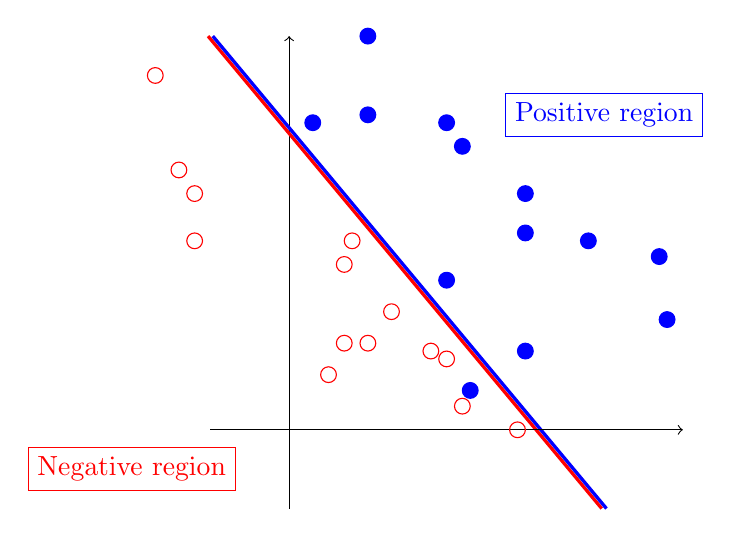
\begin{tikzpicture}
\draw[->] (0,-1) -- (0,5);
\draw[red, very thick](-1.03,5) -- (3.97,-1);
\draw[blue,very thick](-0.97,5) -- (4.03,-1);
\draw[->](-1,0) -- (5,0);
\path (-2,-0.5) node[draw,red]{Negative region};
\path(4,4) node[draw,blue]{Positive region};

\draw[blue,fill=blue] (3,3) circle(0.1cm);
\draw[blue,fill=blue] (3,2.5) circle(0.1cm);
\draw[blue,fill=blue] (3,1) circle(0.1cm);
\draw[blue,fill=blue] (2,3.9) circle(0.1cm);
\draw[blue,fill=blue] (2.2,3.6) circle(0.1cm);
\draw[blue,fill=blue] (1,4) circle(0.1cm);
\draw[blue,fill=blue] (1,5) circle(0.1cm);
\draw[blue,fill=blue] (0.3,3.9) circle(0.1cm);
\draw[blue,fill=blue] (2,1.9) circle(0.1cm);
\draw[blue,fill=blue] (3.8,2.4) circle(0.1cm);
\draw[blue,fill=blue] (4.8,1.4) circle(0.1cm);
\draw[blue,fill=blue] (4.7,2.2) circle(0.1cm);
\draw[red,fill=none] (1,1.1) circle(0.1cm);
\draw[red,fill=none] (0.7,2.1) circle(0.1cm);
\draw[red,fill=none] (2,0.9) circle(0.1cm);
\draw[red,fill=none] (2.9,0) circle(0.1cm);
\draw[red,fill=none] (0.7,1.1) circle(0.1cm);
\draw[red,fill=none] (0.5,0.7) circle(0.1cm);
\draw[red,fill=none] (2.2,0.3) circle(0.1cm);
\draw[red,fill=none] (1.3,1.5) circle(0.1cm);
\draw[red,fill=none] (1.8,1.0) circle(0.1cm);
\draw[red,fill=none] (0.8,2.4) circle(0.1cm);
\draw[red,fill=none] (-1.4,3.3) circle(0.1cm);
\draw[red,fill=none] (-1.7,4.5) circle(0.1cm);
\draw[red,fill=none] (-1.2,3.0) circle(0.1cm);
\draw[red,fill=none] (-1.2,2.4) circle(0.1cm);
\draw[blue,fill=blue] (2.3,0.5) circle(0.1cm);
\end{tikzpicture}
\caption{Linear separability.}
\label{fig:linsep}
\end{figure}

In practice, as well as in the example shown in Figure~\ref{fig:linsep},
perfect performance is rare, because real world problems are usually
not linearly separable, so some misclassifications remain, and
training is stopped when the number of remaining mistakes has stayed
stable for long enough.  When this happens, we are probably doing as
well as is possible on the training set, but does not give us
certainty about how well we will do on an unseen test set.  If the
test set and the training set are similar enough, a perceptron that
does well on the training set will also do well on the test set.
Unfortunately, we are not completely sure how similar the test set
will be, so there is an element of uncertainty in our guesses about
how well we will do.

The perceptron is an algorithm for training a \keyword{linear
  model}. The technical details of how linear models work would take
us too far afield, but the discussion of linear separability above is
part of the story.  The final weights can be understood as saying
something about the importance of each piece of evidence in a combined
solution to the classification problem. When there are a large number
of potentially useful features in a classification problem,
researchers have discovered that linear models often work well. The
perceptron algorithm is not the only way of training linear models, or
necessarily the best, but it is a good starting point for exploration.

\subsection{Modern document classification techniques}
\largerpage
The perceptron uses error-driven learning: The model reads in the training data (featurized as a vector), sends it through a series of nodes associated with weights, outputs  a prediction (spam or ham), and checks whether the prediction was correct.  If the prediction is wrong, the weights of each node are updated to move the predictions in the direction of the correct answer.

The same basic idea underlies many more sophisticated methods which have transformed language technology in recent years.  In \keyword{deep learning}, we can add intermediate layers of nodes in between the input layer and the output layer of the perceptron, to create a ``deeper'' \keyword{multi-layer network}. Such additional layers allow for more complex calculations about how different words interact with each other; for example, a multi-layer network could capture the idea that the words \exword{pain} and \exword{medicine} might be innocuous individually, but indicative of spam when they co-occur.

Such models are called \keyword{neural networks}, because the network of nodes takes inspiration from the way that firing neurons in the human brain work together to create complex behavior, and because neural networks evoke the brain's capacity for learning and abstraction.

Another way to improve our model is to use a more elaborate representation of the input features.  If we represent a document as just a bag of words, then the words \exword{pills} and \exword{medicine} have nothing in common with each other; they are each associated with a different column of a term-by-document matrix.  But we are obviously missing a key insight here -- \exword{pills} and \exword{medicine} have somewhat similar meanings.  How do we know?  They are not strictly synonyms, but they can be used in similar contexts -- \exsent{take some pills}, \exsent{take some medicine}; \exsent{pain pills}, \exsent{pain medicine}.  We saw in \chapref{ch:textasdata} that we can represent words as vectors such that words occurring in similar contexts, such as \exword{pills} and \exword{medicine}, have similar vectors.


In fact,  \textit{pills} and \textit{medicine} have similar meanings and co-occurrence patterns not just in  spam/ham emails, but also in English text as a whole.  So, rather than just capturing what words pattern similarly within our specific dataset, we might want to use \keyword{pre-trained} word embeddings that were built on a large amount of general-purpose English text (for example, Wikipedia), and feed that information into our model alongside a small set of labeled spam and ham emails.  That way, our model has access to a lot of general information about English in addition to specific information about spam and ham.  This strategy is called \keyword{transfer learning}: Our model is given some useful general information, such as the fact that \exword{pills} and \exword{medicine} have similar meanings, and transfers it to the specific task of spam detection. 


In 2018, the idea of pre-training and transfer learning was taken to a new extreme when a team at Google (led by Jacob Devlin) released a model known as \keyword{BERT} \citep{Devlin-etal:2019}.  Rather than just capturing information about which words are similar to each other, BERT was designed to represent a massive quantity of information about English-language text, which can be transferred to a variety of specific tasks, including text classification. 

BERT is a neural network that is originally trained to do two specific tasks, (i) masked word prediction and (ii) next sentence prediction, using a huge amount of data, such as the whole of English-language Wikipedia.  In \keyword{masked word prediction}, the researchers randomly blanked out 15 percent of the words in the text (illustrating here with a sentence from the English Wikipedia page on lions), and trained the model to choose the right word to fill in the blank.  In other words, in the pre-training phase, the model makes a prediction, then checks to see if the prediction matched the original Wikipedia text, and then updates its weights to do better next time, until it gets very good at filling in the blanks of sentences.

\ea  One of the most --- recognised animal symbols in human culture, the lion has --- extensively --- in sculptures and paintings, on national ---, and in contemporary --- and literature.
\z


How would you fill in these blanks?  More importantly, what knowledge do you draw on to make an educated guess?  (The missing words are \exword{widely, been, depicted, flags,} and \exword{films}.)


You probably considered the words immediately to the left and right of the blank, but also other words in the sentence, its structure, and its overall meaning.  To fill in the word \exword{depicted}, you may have considered that the syntactic context requires a past participle, and that depictions are related to symbols and paintings. We already saw in \chapref{ch:call} that such fill-in-the-blank exercises are also used to test the knowledge of human language learners.  By learning to fill in the blanks correctly, the idea is that BERT approximates that same knowledge.  



In \keyword{next sentence prediction}, the researchers randomly paired some sentences with the sentence that actually comes next in the text, and paired other sentences with a randomly chosen sentence from elsewhere in the data (again illustrating with Wikipedia text).  The model was trained to decide whether a given pair of sentences indeed occur next to each other or not.  In a sense, this is a text classification task -- the model is given a two-sentence text and classifies it as either cohesive or disjointed.

\ea Typically, the lion inhabits grasslands and savannas, but is absent in dense forests. // It is usually more diurnal than other big cats, but when persecuted it adapts to being active at night and at twilight.



\ex Typically, the lion inhabits grasslands and savannas, but is absent in dense forests.  // Despite the name, shellfish are not actually fish, but are simply water-dwelling animals.

\z 

How would you decide which sentences match and which do not?  What knowledge do you use?   (The sentences about lions indeed occur next to each other in Wikipedia; the sentence about shellfish is from a different page.) You probably thought about how the pronoun \exword{it} could refer back to the singular noun \exword{lion}; how \exword{cats} are related to lions, how the daily habits of an animal might be described in the same paragraph as its habitat, and how shellfish, fish, and water are not particularly related to the lions, savannas, and forests discussed in the prior sentence.  By learning to decide which sentences match, the idea is that BERT approximates that same knowledge. 

Stepping back, why would researchers take the trouble to train a network to fill in blanks and to decide whether two sentences go next to each other?  These tasks are not particularly useful in a commercial context!

One major advantage of these tasks is that the labels required for training -- the missing words and the contiguous sentences -- are already provided by the text itself, unlike human labels for ham and spam, so it is easy to train BERT on a massive amount of text.  The other major advantage is that these tasks require BERT to ``learn'' a great deal of rich information about English text, both at the word level and the sentence level.  For example, BERT will learn that \exword{pills} and \exword{medicine} are similar because they are both often good candidates to fill in the same missing word in a sentence.  Moreover, masked word prediction leads BERT to represent not just the overall distribution of a word type such as \exword{pills}, but the context of each word token -- the fact that \exword{pills} means something different in a sentence like \exsent{This sweater pills in the wash} versus \exsent{Take these pills for your headache}.  Each token of \exword{pills} receives a different vector representation.

Even if masked word prediction and next sentence classification are not particularly useful on their own, the idea is that they serve as a powerful pre-training regimen.  Instead of just importing pre-trained word embeddings into a spam-detection model, the idea is that we can read in the entire BERT network, pre-trained on masked word prediction and next sentence prediction, and then add a few layers on top of it which we train on labeled spam/ham data to do spam detection (known as \keyword{fine-tuning} BERT's pre-trained knowledge for this specific task).  This way, the model will not only have access to a small set of spam/ham data, but is also able to transfer a massive amount of general information about English.  The use of such general information is known as \keyword{transfer learning.}


To use a sports analogy,  imagine that you want to train, as  efficiently as possible, to compete at many different speed sports.  (BERT is trained, as efficiently as possible, to compete at many different language-related tasks). You decide to focus on push-ups and squat jumps.  (BERT focuses on masked word prediction and next sentence prediction.) These exercises are easy to do anywhere, requiring no  specialized equipment (for BERT, these tasks require no  specialized labels).   They are also very challenging exercises that work out your entire body, your muscles and your cardiovascular system, explosiveness and endurance (for BERT, these tasks require knowledge about the structure, meaning, and statistical tendencies of English text). You do an enormous number of push-ups and squat jumps,  several hours a day for months (BERT trains on masked word prediction and next sentence prediction on an enormous amount of data.)  Once you have trained to be very good at push-ups and squat jumps, you will still need specialized practice to compete at sports such as running, swimming, or rowing (BERT still requires some fine-tuning to do spam detection using labeled spam/ham data.)  But the athleticism developed from push-ups and squat jumps is highly transferable, and this training regimen has made you a powerful, versatile athlete well-prepared to succeed at many different sports.  (The information gleaned from masked word prediction and next sentence prediction is highly transferable, and BERT's training regimen has made it a powerful, versatile  representation of language well-prepared to succeed at many different tasks.)

Using the power of transfer learning, BERT and its descendants form the basis of modern document classification, and in many tasks such models are stunningly accurate.




\subsection{Which classifier to use?}

We have toured many different techniques for classifying documents, walking through the simple examples of naive Bayes and the Perceptron, and then sketching the intuition used in the elaborate models of today.  With so many options, which one should you use?

Coming back to our medical discussion of payoffs and priorities, it depends on what you are trying to do.  If your goal is to get the best performance, and if you have time and programming skills, you may want to use a model such as BERT that leverages transfer learning.  If you are intellectually curious  about which specific words are most associated with which labels, you may want to use naive Bayes, which can show you the spam:ham odds ratio associated with a particular word; thanks to its simplicity, naive Bayes is  more \keyword{interpretable} than more elaborate techniques.  You may also want to try out a simple model and see how well it does as a baseline, and then decide if you need something more complex.

To get started on a practical level, you might use the Pandas library in Python to format your data as a matrix (expect to spend some time on such formatting!), and Google's TensorFlow package in Python to try out different machine learning techniques.  If you search the web, there are lots of resources and sample code notebooks to help you get started.



% The main reason for including brief discussion of the perceptron is to show that there is more than one way to do machine learning. Intuitively, the idea of collecting statistics over a collection of examples is very different from maintaining a collection of weights that are updated in a mistake-driven way. But at a deeper level, both of these approaches are supervised learning, and it is likely that they will perform similarly a lot of the time. Usually, the most important part of a machine learning solution is the choice of features that provide information about the distinctions that we want the classifiers to learn about, and the choice of which classifier plays an important but secondary role. Our advice is to try a few off-the-shelf classifiers and choose the one which seems to be working best for your problem. A toolkit containing state-of-the-art implementations of many classifiers is Weka (\url{http://en.wikipedia.org/wiki/Weka_(machine_learning)}), which is written in the programming language Java and is fairly easy to use.

%Weka also contains software for predict numeric continuous values, such as the numbers of stars in a movie review (here we are imagining that the movie review site produces really detailed ratings, not just whole numbers of stars, and that the rating could be a decimal like 3.72) .  Predicting continuous values from features is called \keyword{regression}. By contrast, the perceptron and Naive Bayes produce predictions from a fixed set of discrete values, often just \emph{yes} or \emph{no}. Programs that predict discrete values are called \keyword{classifiers} in the machine-learning literature, and the term \keyword{classification} is used when it is important to make clear that they are predicting discrete rather than continuous values.

% Another way of making our general point is that the choice of classifier should be based on thinking about the \keyword{context of use} of the technology. While programmers will certainly care about the details of how the algorithms work, users and managers will care more about what the system can do, what kind of errors it will make, and how this fits in with the real world needs of the organizations or other clients who want to use the technology. One of the reasons for the substantial emphasis on evaluation in this chapter is that good evaluation focuses attention on the tradeoffs that are involved in really using technology.  In the final section of this chapter, we provide a brief case study to illustrate how document classification technology is actually deployed.  The important lesson is not that the authors think the technology is cool, although we do think it is, but that we think that it is useful for finding good solutions to real-world problems.

\section{Some other applications  of machine learning}

Stepping back, machine learning is a remarkably powerful idea with important applications far beyond text classification.  Classification -- mapping a vector of features to a label, chosen from a finite set of possible labels -- is also used in computer vision, where we can represent an image as a vector of pixels and learn how to label it as a cat or a dog, or perhaps learn to map an image of a handwritten digit to the number (0, 1, 2, 3, 4, 5, 6, 7, 8, or 9) that it represents.  We can also represent a credit card transaction as a vector of features (the time of day, the type of store, the location, the price, information about the cardholder's usual habits) and learn to label it as fraudulent or legitimate.  And so on.

As we mentioned above, classification is an example of \keyword{supervised learning}, because we give the computer some ``right answers'' (correctly labeled spam/ham emails) and train it to generalize those labels to new data.  Apart from classification, the other main type of supervised learning is \keyword{regression}; there, instead of a label, our goal is to predict a continuous numerical value. To use a language example, we could train a model to read an essay and give it a score out of 100.  Here, too, the model learns to generalize from ``right answers'', but these would take the form of featurized essays that have already been correctly scored.  (Before we turn this model loose on real student work, we would want to make sure that it was not reproducing some sort of bias that could give unfairly low scores to certain students!)  We could also represent a house as a vector of features (its location, square footage, year it was built, number of bathrooms) and learn to predict its price.  And so on.

In contrast, \keyword{unsupervised learning} is used when we do not give the model any ``right answers'' -- because we do not have the resources to collect labels, or because we do not even know what such labels would be.  We saw an example of unsupervised learning in \chapref{ch:textasdata} in the context of topic modeling: A topic modeling algorithm is not given any labels to generalize, but is instead designed to identify meaningful groups of words and documents (each associated with topics) in a bottom-up manner.  Another type of unsupervised learning is called \keyword{clustering}, in which a model is asked to group similar data points together -- for example, clustering together documents that are similar to one another according to some sort of vector representation of the words used therein.   (Outside of text, we could also cluster together similar images, similar houses, and so on, as long as these are represented as vectors.)  With no need for expensive labels, clustering is useful for exploring a large dataset that you do not have time to read.  The model does not give names to the clusters (although a human reader may try to), and the main disadvantage is that the clusters may not be intuitive; perhaps it would put some social emails into a cluster dominated by work emails, if the social emails happen to mention calendar dates.

We hope that this brief overview has offered a framework to understand the power of machine learning, which will come up again in this book and perhaps in your life more broadly.

% The reader will be able to notice that articles in a given cluster share something, such as being about sports, but the algorithm would be just grouping articles, not trying to name the clusters. The big plus of this approach is that you do not need a training set, so there is no costly process of going through labeling up the articles. The big negative is that the clusters might not be that intuitive. For example, if you cluster common words, one cluster often turns out to be the words \exsent{Monday}, \exsent{Tuesday}, \exsent{Wednesday}, \exsent{Thursday}, with \exsent{Friday} off in another cluster. This is because Friday is the only weekday that frequently turns up following \exsent{Thank goodness it's \ldots}.


% reinforcement learning.....
% video games?, robots????,
% intelligent behabior in complex environments
% agent, environment, reward, state
% policy gradients.... 
% needs to learn a policy for acting in various environments to get the best reward.
% state, action, reward.
% if something works, you do it slightly more often - you update your policy gradient.
% but maybe if a reward requires MANY different actions in sequence, you will never get there randomly, 
% or you will never know where you went wrong if you fail (maybe you did a lot right, but you may not know that) - `credit assignment problem'
% can also build in interim rewards, that are not the final reward???? `reward shaping???'
% but takes a lot of work
% reinforecement learning is hard. 
%
% action affects environment, environment affects state, state affects action
% action also leads to a reward.... 
% given a certain state, what action is likely to lead to a reward
% try a few different things, see what works -- exploration


% what is reinforcement learning
% need to add in somewhere about OVERFITTING.... 
% WHAT HAPPENED TO THAT PART, add it back in

%

\section{Sentiment analysis}

With this background, we can come back to another key application of text classification -- classifying texts by their emotional valence, also known as \keyword{sentiment analysis}.

On websites such as IMDB (Internet Movie DataBase) and Amazon, people can write a review of a movie or product, and  annotate it with a star rating: 5/5 or 10/10 stars if they love it, 0 stars if they hate it -- helpfully providing labels for those of us interested in sentiment analysis!  Drawing on our discussion of machine learning, we could train a regression model to predict a review's star rating out of 10, or train a classifier to assign a label of positive or negative (or perhaps positive, negative, neutral).

Here are two IMDB reviews for \exword{Parasite} (2019), the first Korean film to win Best Picture at the Academy Awards.  Without knowing the star rating, what clues do you use to figure out whether each review is positive or negative?

\ea The most original film of 2019 and it is wickedly funny and darkly disturbing all at the same time. Class warfare at its best.


\ex  I truly don't know what I missed but this was just not my cup of tea (or my mom's) and it felt unnecessarily gruesome and strange rather than masterful and sharp. Instead of awaiting the next moment with excitement and suspense, I found myself cringing at the actors' performances as they weren't believable and was confused at how poorly-written the dialogue was. 

\z 

 The first review is positive (10/10 stars), and the second review is negative (1/10).  The positive review uses positive words -- \exword{original, funny, best} -- along with the slightly negative word \exword{disturbing}; it also uses superlatives (\exword{most, best}) and intensifiers (\exword{wickedly,  darkly}).  The negative review uses some negative words -- \exword{strange, cringing, poorly-written}.  It also uses some positive words (\exword{masterful, sharp, excitement, suspense, believable}), but some of them are negated by \exword{instead of} and \exword{weren't}.  In fact, as shown by \citet{Potts:2010} and discussed in \chapref{ch:textasdata}, negation itself (\exword{don't, not, unnecessarily, weren't}) is common in  negative reviews as a whole, which is intriguing because you might have expected negation to have a purely logical meaning rather than an emotional one.


Just as with spam detection, we can feed labeled positive/negative reviews into a classifier (naive Bayes, the Perceptron, or a fancy classifier using transfer learning) and train it to classify the sentiment of future reviews.  The classifier will probably be more accurate if it ``knows'' that most of the positive words in the negative review are semantically negated.  One quick-and-dirty technique \citep{DasChen:2007} is to prepend \exword{NOT} to every word that falls between negation and the end of a sentence or clause -- \exsent{they weren't NOTbelievable} -- before making a bag-of-words.  This way, \exword{believable} and \exword{NOTbelievable}  count as two different words, one of which probably predominates in positive reviews, the other in negative ones.  On reviews like the two we just read, a classifier should be quite accurate.

In addition to measuring the accuracy of our classifier, it is also worthwhile to examine the documents that it classifies incorrectly (\keyword{error analysis}).  Such hard-to-classify documents may illuminate interesting subtleties in the data, and help us understand what the classifier ``knows'' and doesn't ``know''.  

For example, we tried one classifier that was correct about the positive and negative reviews discussed above, but still mis-classified as positive a review from the legendary film critic Roger Ebert which is actually humorously negative:



\ea  The director [of the 2004 film \exword{Catwoman}], whose name is Pitof, was probably issued with two names at birth and would be wise to use the other one on his next project.
\z 





To do an error analysis, we can ask ourselves:  

\begin{itemize}

\item \emph{Why is this review difficult to classify?} Most likely, because it does not use any negative-sentiment words; the negative opinion is inferred by complex hypothetical reasoning.  To understand why the \exword{Catwoman} review is negative, we have to understand that the director would want to use another name on his next project because the  project with his original name was bad; but that logic is not spelled out in the review itself.

\item \emph{What do these errors tell us about the subtleties of our data?} This review shows that language is complicated! Negative sentiment does not just come from negative words, but also arises when sentiment-neutral language is used to describe a state of affairs that we recognize extra-textually as negative.
 

\item \emph{What do these errors tell us about what the classifier ``knows'' and doesn't ``know''?}  The classifier performs well on reviews that state their sentiment outright in words, but does not fully capture the complex extra-textual reasoning required to decode Ebert's snark.

\end{itemize}

Just like spam filtering, sentiment analysis can be used for practical purposes, for example, to track consumers' sentiment towards one's company on social media.  But it can also be used for purely intellectual explorations in the areas of digital humanities, computational social science, and corpus linguistics introduced in \chapref{ch:textasdata}.  Within digital humanities, one could track the sentiment of sentences in a novel from beginning to end or the sentiment of sentences about various characters.  In computational social science, one might explore the sentiment of news articles or statements by politicians across the ideological spectrum.  In corpus linguistics, one could explore how a word's sentiment (or that of its collocational context) might change over time in historical data, as when the word \exword{mistress} changed from meaning ``Mrs.'' to meaning ``a woman in an extramarital affair'' \citep{TraugottDasher:2001}.  Returning to the theme of how computers can extract meaning from text,  sentiment analysis represents one way that computers can capture emotional meaning.

% talk about how it is also important to do ERROR ANALYSIS
% this will help us understand the classifier and why it is doing what it is doing
% what is hard and why?
% add in the thing about overfitting too.
% 

\begin{tblsfilledsymbol}{\underthehoodsubsection{Benchmarks and leaderboards in NLP}}{glass}
\begin{underthehood}

BERT was recognized as a striking advance because it shot to the top of various \keyword{leaderboards} tracking performance on various \keyword{benchmarks} in natural language processing.  These benchmarks represent standardized tests, similar to the Scholastic Aptitude Test (SAT) used for college admission in the United States,  designed to test difficult tasks in language understanding.  Just as the SAT publicizes practice problems but not the real test that students are graded on, these benchmarks provide training data but evaluate models for their performance on an unseen test set.  Moreover, similar to how SAT measures quantitative and verbal skills in the same test, a \keyword{combined benchmark} brings together several different tasks into a unified scoring framework.  The creators of such benchmarks also gather human annotations from web platforms such as Mechanical Turk to compare for the models' performance.

Such benchmarks are common in computer science; in the field of computer vision, the ImageNet benchmark \citep{Deng-etal:2009} tests models for whether they can correctly assign text labels (\exword{strawberry, dog}) to images.  It took about seven years for computers to compete with human performance on the ImageNet data, but recent progress has accelerated.  In NLP, it took only one year for the combined GLUE (General Language Understanding Evaluation) benchmark of \citet{Wang-etal:2018} to be deemed too easy for models such as BERT, motivating the more difficult SuperGLUE version \citep{Wang-etal:2019}.  

SuperGLUE brings together eight different tasks meant to test a model's ability to reason about English text.  For example, drawn from \citet{Dagan-etal:2005}, the RTE (Recognizing Textual Entailment) task asks whether \REF{reagan} entails \REF{normandy} (it does not).  


\ea \label{rte} \ea \label{reagan} Reagan attended a ceremony in Washington to commemorate the landings in Normandy. 
    \ex \label{normandy} Washington is located in Normandy. [False; not entailed.]
    \z
    \z 


In fact, there are two different routes to the correct answer in \REF{rte}.  Leveraging knowledge about events, one could reason that a ceremony can take place in a different location from the event it commemorates.  Or one could use the geographical fact that Washington is in the United States while Normandy is in France.  So perhaps \REF{rte} is too easy!

To make more difficult benchmarks, some researchers gather \keyword{adversarial} examples, explicitly asking gig workers to try to fool the model.  The adversarial example \REF{adversary} is tricky for a model of textual entailment   \citep{Nie-etal:2020} because it requires the model to infer that the \exword{assassination} of a journalist entails \exword{another individual laid waste to} him -- requiring complex reasoning about how the abstract event-denoting noun \exword{assassination} can be paraphrased by a sentence using an obscure idiom (\exword{laid waste to}).


\ea \label{adversary} 
    \ea \label{roberto} Roberto Javier Mora Garc\'ia (c. 1962 – 16 March 2004) was a Mexican journalist and editorial director of \exword{El Ma\~nana}  [\ldots] prior to his assassination.
    \ex  \label{waste} Another individual laid waste to Roberto Javier Mora Garc\'ia. [True; entailed.]
\z
\z 

Benchmarks are important for measuring progress and challenging the research community to improve.  But like any standardized test, they have been criticized.  For one, SuperGLUE (General \emph{Language} Understanding Evaluation)  only really measures \emph{English} understanding, further cementing English as a hegemonic standard.  Moreover, as argued by \citet{EthJurafsky:2020}, benchmarks ignore progress on other important dimensions such as fairness (avoiding social biases) or compactness (aiming for smaller, more energy-efficient models).  They don't necessarily reward the theoretically interesting insights or explanations sought by linguists.  Because NLP benchmarks prioritize objective true-or-false questions, they do not extend easily to models offering open-ended language generation.   Therefore, each researcher has to decide for themselves how much they prioritize benchmarks versus other definitions of success.


\end{underthehood}
\end{tblsfilledsymbol}



\section{Consequences}


Some challenging text classification tasks are not commercially applicable, but still provide insight into the power and limits of classifiers, and the subtleties of the information conveyed in language.  What accuracy would you expect from a classifier that tries to predict whether a comment is sarcastic or serious (perhaps using as labels the \exword{/s} symbol that some web writers use to convey sarcasm)? What about a classifier that reads narratives on the Reddit web forum r/AmITheAsshole, where people describe their conduct and ask readers for a moral judgment, and tries to predict whether a person is deemed to be ``the asshole'' or ``not the asshole''?  What about a classifier that reads sentences and tries to label them as ``grammatical'' or ``ungrammatical'' following the labels used in linguistics textbooks \citep{Warstadt-etal:2019}?  By comparing human and computer performance  on such tasks, we learn more about the ``intelligence'' of both humans and computers, as well as the subtleties of these data.

Other text classification tasks pose challenging ethical questions.  What if you tried to  detect automatically which job candidates should get an interview based on their r\'esum\'e, training on previously submitted r\'esum\'es of people who were or were not interviewed?  For a company that receives thousands of   r\'esum\'es a day, many tedious hours of human labor could be saved by automating this process.  But what if the classifier learns that the word \exword{lacrosse} increases a person's chance of an interview, or that the word \exword{community college} decreases it, when neither of these socio-economic signals actually relates to the job description?  Our system could end up reproducing harmful inequalities.  (Would a human be any less biased?  How could the performance of both human and automated r\'esum\'e-screeners be made anti-discriminatory?)

Moreover, how does text change when its authors know that it will be run through an automatic classifier? How do spammers adjust spam to slip through spam filters? How do job applicants tailor their r\'esum\'es to pass automatic screenings?  How might such classifiers need to be updated to account for these new strategies?


Armed with the basics of machine learning and its application to document classification, you have a powerful set of tools for understanding the world.  But you also have to think critically about linguistic complexity, human priorities, and ethics in deciding how to apply these tools.


\begin{tblsfilledsymbol}{Checklist}{test}

\begin{itemize}
\item Give examples of text classification tasks.  
\item Brainstorm several business applications of text classification.
\item Give examples of other classification tasks beyond the realm of documents.
\item Explain specificity, sensitivity, and their relevance for text classification.
\item Discuss what constitutes ``success'' for a classifier, using quantitative notions such as sensitivity and specificity as well as  one's qualitative priorities.
\item Explain base rates and the base rate fallacy.
\item Define over-fitting and its significance for machine learning.
\item Explain how naive Bayes classification works.
\item Explain how the Perceptron classifier works.
\item Sketch the idea of transfer learning.  
\item Describe the two tasks used to train BERT and explain why they were used.
\item Distinguish supervised versus unsupervised learning.
\item Analyze which tasks and examples you would predict to be easier or harder for a classifier. 
\end{itemize}
\end{tblsfilledsymbol}



\begin{tblsfilledsymbol}{Exercises}{pencil}
    


\begin{enumerate}

\item  Expanding beyond consumer technology such as spam filters, think back to digital humanities and computational social science as discussed in \chapref{ch:textasdata}.  How can classification tools be used in these realms?  To help you get started, consider how you might train a classifier to label text for its genre; its sentiment; its author (out of a closed class of authors); or for its author's gender, political party, or native language.  How would you find such labels to train your classifier?  To what extent do you think that a classifier could learn to predict these labels from the text?


\item  Sentiment analysis makes use of user-provided training labels; users annotate their own review with a star indicating its sentiment.  What other sorts of user-provided labels are available in online text today? How could they be used?



\item  Many advertisements and mass mailings probably make it into your inbox rather than your spam folder.  Do you consider these emails to be spam or ham (or something in between)?   How do you think an email system should handle them?


\item 
  \begin{enumerate}
\item Table~\ref{tab:payoffs} gives a calculation of the payoffs associated with each outcome of the medical test in the extended example. Put this together with the population statistics in Table~\ref{fig:diagnostic3}
to calculate the overall payoffs from: (a) always running the test, and (b) never running the test. Which is the more cost-effective policy for the hospital ? 
\item We carefully set up our example so that everyone was cured and the only effect of your decision is financial, but of course the mathematics also applies to decisions where much more is at stake. 
Now that you have learned about false positives, true positives, payoffs and the rest, you have the conceptual tools to understand the tradeoffs that are involved in deciding whether a country should
have a policy of offering mammography as a general screening tool for breast cancer. We recommend that you find information about this online, read about it, and see what you think. Do not
stop after the first article you read. It is a controversial issue, and you will find sensible articles advocating both for and against general screening. 
\end{enumerate}

\item  You are the owner of a spam filtering service: 

\begin{enumerate}
\item
Currently, your server gets 2000 spams per hour and only 500
good messages. The filter classifies 95 percent of the spams correctly, 
and misclassifies the other 5 percent. It classifies 99 percent of the good
messages correctly, and misclassifies the other percent.
Tabulate the results: How many false positives and how many false
negatives do you expect to see each hour?
Calculate 
 the precision, sensitivity, and specificity of the spam 
filter.
\item
You receive word
that a criminal gang is planning to double the amount of spam that it
sends to your server. There will now be 4000 spam messages per hour
instead of 2000. The number of good messages stays unchanged at 500.
In your marketing literature, you have quoted
the precision, recall, sensitivity and specificity of your spam
filter. You assume that the misclassification rates will stay the
same (5 percent for spam, 1 percent for good messages).
Should you put in a call to the technical writing department
warning them that the literature will need to be revised? Why or why
not? And if so, what will need to be revised?
\end{enumerate}

\item  Continue the calculation from Section \ref{sec:nb}.
	 Assume that the next word in the email is \exsent{cookie}. Using the frequency statistics from Table~\ref{spam:data},
	carry out the next step of the calculation. What is the cumulative ratio for spam/non-spam?

\item  Your colleague labels product reviews (\exsent{Sturdy and comfortable, this cot folds up and out of sight with minimal effort}) based on the gender of the review's author, mapping the author's self-disclosed name (\exword{Sarah, Ralph}) to census data about the likely gender of people with that name.  Your colleague then trains a classifier to label reviews for the gender of the author.  The colleague's goal is to label the author gender of anonymous reviews, which could provide demographic marketing data to sellers.  What comments would you offer this colleague -- about the difficulty of the task, the assumptions underlying it, and the real-world utility of the classifier?
	

\item   Read some posts on Reddit/AmITheAsshole and discuss what knowledge would be required to correctly label the author as ``the asshole'' or ``not the asshole''.  Do you think that modern LLMs will succeed at this task? Can you search the literature for recent discussion or try to test this prediction yourself?
	

\item  Try out some web demos of sentiment classifiers -- you can find the most up-to-date ones by searching the web for \exsent{sentiment analysis demo} -- and try to ``break'' the classifier by giving it difficult examples.

\end{enumerate}
\end{tblsfilledsymbol}



\begin{tblsfilledsymbol}{Further reading}{book}
    
The statistical approach to spam filtering was popularised by Paul Graham's ``A Plan for Spam''.\footnote{\url{https://www.paulgraham.com/spam.html}, accessed 2024-04-18.} His article, which has aged very well, is an excellent starting point for learning about the technology and sociology of spam.  
  
  \citet{DBLP:journals/ftir/PangL07} offers a comprehensive introduction to opinion-mining and sentiment analysis. 
  
  The discussion of base rate fallacy is based on \citet{BarHillel:80}. Cognitive biases are discussed in the literature on psychology and behavioral economics.  
  
  On websites such as YouTube, Medium, and GitHub, you can find many excellent tutorials and example code about sentiment analysis, document classification,  transfer learning, and BERT.

\end{tblsfilledsymbol}

\chapter{Searching}
\label{ch:searching}

\section{Introduction}
\label{sec:search-intro}

\subsection{Finding an old friend}

One day, you happen to remember a childhood friend of yours, Katie Smith from Denver, Colorado, whom you haven't thought about in  years.  You were best friends in second grade, before she moved to a different school.  What is she up to now?  You type \exword{Katie Smith} into a search engine.  On the right side of the page, you see a panel about a basketball coach with the same name, linking to her Wikipedia page -- but she is a different, more famous Katie Smith.  On the left, you see a list of links to web pages, mostly about the basketball coach, and a few other individuals with the same name, but still nothing about your childhood friend.

What is the problem here?  You know the name of your friend; you know she is probably on the internet somewhere; so why is it so hard to find what you want? 

Unfortunately, Katie Smith has a very common name, so results about your childhood friend are overwhelmed by results about other people with the same name.  And anyway, Katie may have changed her name (maybe she got married, maybe she started going by Kathryn  as an adult; you haven't seen Katie in a decade, so who knows?)

Although this example may seem trivial, it is genuine, 
it corresponds to a real information need, and it reveals some of the problems that can
arise when we search the internet.

Consider what the options are for finding the information we want:
\begin{itemize}
\item Keep querying the search engine: Try further queries such as \exword{Kathryn Smith}, \exword{Katie Smith Colorado}, \exword{Katie Smith Denver}, \exword{Katie Smith} plus the name of your elementary school.

\item Leave the search engine to visit a social site with search functionality, such as LinkedIn, Instagram, or Facebook; maybe you'll have some connections in common with her, which could help you find her.

\item Call your parents, who were friends with Katie Smith's parents and might know something.

\end{itemize}

There is no single right answer. If you can find the right search query, maybe the search engine will work; if your online social connections include other people from second grade, then a social site might work.  

But to find this information online, you have to know what resources are available, and how to search through them.  This chapter provides an overview of how people use computers to retrieve information that they want (\keyword{search}, also known as \keyword{information retrieval}),  to  find answers to questions (\keyword{question answering}), and to browse for things  -- music, movies, friends, web posts -- that they didn't even know they wanted (\keyword{recommendation systems}, also known as \keyword{recommender systems}).  


%We will focus on searching in \keywordAs{written texts}{written text}, but one might also wonder about the possibility of searching through \keyword{speech}.  After all, it would be extremely useful and time-saving to be able to find a particular sentence spoken in a podcast, especially if no transcript exists, but only an audio file.  This type of searching is  not readily available yet.  But it is now possible to request information in a spoken medium (\exsent{Okay, Google, what's the weather today?}) -- where the query is mapped from speech to text, the answer is found in a textual database, and then mapped from text to speech --   and receive a spoken answer.



\subsection{Information need}

\label{sec:information-need}

The task of information retrieval begins with an \keyword{information need} -- the information that the searcher is searching for.  An information need is a type of \keyword{intent} -- something that a user wants.  In the case of an information need, the searcher  wants to \emph{know} some information, like \exsent{What happened to my old friend Katie Smith}? or \exsent{When did Mandarin and Cantonese diverge}?    Sometimes, they may want information that is not textual, such as images, videos, the score of an ongoing sports game, or directions on a map.  Other times, they may intend to \emph{do} something, like set a timer, book a flight, or purchase some shoes.  (Or they may want a blend of information and action -- they want to know how much a flight to Guatemala costs, while considering whether to buy one.)   

Once a user has formulated an intent in their mind, they must translate it into a text \keyword{query} to enter into a search engine.  The query may reflect the user's intent with more or less clarity.  If a user types \exword{Chinese history} as their query, maybe they may want the Chinese translation of the word \exword{history}, or maybe they want to read about the history of China or of  Chinese languages.  A well-practiced searcher may know how to clearly formulate their query given their intent, but an inexperienced searcher may be frustrated by results of an ambiguous query.  (A user-friendly search engine may suggest followup queries to help the user clarify their intent -- perhaps based on the search histories of other people who have entered similar queries.)

For many modern search engines, one of the first steps in processing a query is to map it to an \keyword{intent} (\keyword{intent recognition}, also known as \keyword{intent classification}; see \chapref{ch:text-classification} on text classification) -- does the searcher want to shop, to look at maps or images, to translate from one language to another, to use a calculator, or to just read text?  Then the query can be fed to a system specialized for that type of task.  If the searcher wants to \emph{know} something rather than to \emph{do} something, then their intent can be considered an \keyword{information need},  fed to a question-answering system or a search engine built for text documents.


\ea   \ea \label{ex:chinese-history} Information need:    Want to read a short, accessible overview of the history of  Chinese languages.
      \ex Possible queries: 
      \exword{Chinese history, Chinese history language, Chinese historical linguistics, Mandarin Cantonese history}.
      \z
      \z 




\subsection{Evaluating results} \label{sec:evaluating-search-results}

A search begins with an information need and ends when the user has succeeded in filling it.  How do we measure success?

Of course, we could just ask the user if they are happy, or survey several hundred users in a user-experience study.  We could also use implicit behavioral measures of satisfaction, like whether the user clicks on a page and stays there for a while before ending their search session (suggesting that they found what they wanted), or how many people choose to use the search engine (suggesting that they like it).    But it is also valuable to have an explicit, quantifiable evaluation metric that can be computed automatically without conducting a new round of user testing each time.

The simplest, most widely used automatic evaluation metrics for information retrieval are \keyword{precision} and \keyword{recall}.  Precision can be defined as \exsent{the percentage of the documents returned that are relevant}: For example, imagine that a search engine returns 400 pages for a query, 200 of which are actually relevant to the query (and thus, ideally, to the information need that underlies it).  In this case, precision is 50 percent, or 200 out of 400.   
\begin{equation}
\mbox{Precision} = \frac{\mbox{Relevant documents that are returned}}{\mbox{All documents that are returned}} 
\end{equation}

In contrast, recall can be defined as \exsent{the percentage of relevant documents that are returned}:  If a search engine returns 200 relevant pages, but there were actually 1000 pages on that topic out there on the
web (we missed 800 of them), the recall is 20 percent (200/1000).  Note that the numerator (200 -- the number of relevant documents that are returned) is the same for both precision and recall.  
\begin{equation}
\mbox{Recall} = \frac{\mbox{Relevant documents that are returned}}{\mbox{All relevant documents}} 
\end{equation}

But how can we know that there are 1000 pages out there, if we can't find them?  Sometimes, information retrieval systems are evaluated on constrained, human-labeled datasets where researchers can be omniscient.   One historically important dataset comes from the Text REtrieval Conference (TREC), a series of queries, documents, and human judgments of whether each document is relevant to each query.  In this toy context, we can calculate the precision and recall for any search engine that runs over these data.  But in real life, it is often impossible to know how many relevant documents are \emph{not} being returned in your search.  So, in practice, while recall is a useful concept, it cannot always be calculated with   certainty.  In contrast, precision can be easily estimated just by looking at the documents that \emph{are} returned.



What would happen if a search engine prioritized \emph{only} precision, and ignored recall?  A search engine could achieve perfect precision by returning only one or two pages that are definitely relevant, while leaving out hundreds of other relevant pages.  But the user may have wanted to see those pages too.

What would happen if a search engine prioritized \emph{only} recall, and ignored precision?  A search engine could achieve perfect recall by returning every single page on the web for every single search: The relevant pages are in there somewhere.  The user will be overwhelmed by irrelevant pages in their search for relevant ones.

Thus, a successful search engine must balance both precision and recall.  Sometimes, researchers use a combined score known as the \keyword{F-measure} to reflect both components at once:  The F-measure is defined as $(2 * p * r)/(p + r)$, where $p$ is precision and $r$ is recall.  In our example from above, our precision was 50 percent (200 of the 400 returned documents were relevant) and our recall was 20 percent (200 of 1000 total relevant documents were returned), so the F-measure would be $({2 * 0.5 * 0.2})/({0.5 + 0.2})$, or 28.5 percent -- indicating that these search results are far from the optimal F-measure of 100 percent.  

But the search engine with the best F-measure is not necessarily the best search engine. In reality, users often do not want to look at the 400 documents returned in our imaginary search, nor even at the 200 relevant ones.  They usually want to glance at the first display page of ten or so results, and then click on  one or two that looks most interesting from a title or snippet that the search engine displays.  In this reality, the results also have to be \keyword{ranked}, so that the ``best'' results show up on the first page.   How do we decide which results are the best?  Perhaps we should recast relevance as a gradient notion rather than a binary one, and give higher rankings to documents that are \emph{most} relevant.  Or perhaps we want to give higher rankings to pages that come from better sources -- perhaps pages from vetted sources; or perhaps those with more traffic, those that were updated recently, or those that a lot of other pages link to.  Perhaps we want to give higher rankings to pages that are most relevant to \emph{this specific user} -- pages that they have visited before, or pages that are popular in their location.  We come back to this idea of \keyword{personalized search} later in the chapter.

However we rank the pages, users  care much more about the top page of results than the rest.  And on the top results page, precision is much more important than recall.  If some of the top-ranked pages are not relevant, the user may become annoyed; however, if some relevant pages are not among the top-ranked pages, the user may not care.  To capture these priorities, search engines can also be evaluated using the \keyword{precision-at-k} metric: Starting at the top and looking at some number $k$ of results, what is the precision of these results?  For $k=1$, we look at the first, top-ranked result.  If it's relevant, then the precision at $k=1$ is 100 percent.  For $k=2$, we look at the second-ranked result.  If it's relevant, the precision at $k=2$ is 100 percent: Two of the top-two results are relevant.  If it's irrelevant, then the precision at $k=2$ is 50 percent: One of the top-two results is relevant.  This metric reflects the fact that precision is more important than recall among the top-ranked results.


\section{Structured data, knowledge graphs, and ontologies}
\label{sec:structured-data}

We begin our tour of information retrieval with  \keyword{structured data}.  For example, the Internet Movie Database (IMDB) is a structured database of the film industry, in which each movie is associated with various \keywordAs{fields}{field} such as title, actors, director, plot summary, and date; and each person is associated with their works, a birth date (perhaps also a death date), and a brief biography.  

Structured data are extremely useful.  If you want to see a list of all the movies by your favorite director, it is probably most efficient to look at the structured list linked from their IMDB profile (or their filmography listed on Wikipedia) rather than just read free-text webpages containing their name.  As another example of structured data, you can find scholarly articles on Google Scholar, which uses a structured representation for authors, dates, papers, and citations, along with the unstructured text of each article. Authors are associated with universities, coauthors, and papers that they wrote; papers are associated with authors, titles, dates, and the papers that they cite and those that cite them.

Outside constrained domains such as IMDB and Google Scholar, web search in general now makes use of structured data in the form of a \keyword{knowledge graph} (also known as an \keyword{ontology}) -- a representation that includes:

\begin{itemize}
  \item \keywordAs{Named entities}{named entities} (people such as \exword{Queen Elizabeth II}, countries such as \exword{Guatemala}, companies such as \exword{Apple}, sports teams such as \exword{The Lakers}, books such as \exword{Anna Karenina}).
  \item Kinds of things, such as those named by nouns (diseases such as \exword{flu}, species such as \exword{dog}, foods such as \exword{potato}).
  \item Events (such as \exword{the Second World War} and \exword{the 2024 Olympics}).
  \item Times (years such as \exword{2024}, dates such as \exword{December 1, 1990}, and intervals of time such as \exword{1900-2000}).
  \item The properties of these entities (people are associated with birthdates, death-dates, and occupations; events are associated with dates as well as key participants; companies are associated with stock prices, CEOs, and the date of  their founding; diseases are associated with prevalence and treatments; foods are associated with their macronutrients).
  \item Relations between entities and events (between a person and their nation of residence; a book and its author;  a person and their spouse;  a person and the schools they attended;  a company and its founder;  a country and its continent; a war and its battles).
  \item And so on.
\end{itemize}

When you search for \exword{Barack Obama} and see a panel containing his picture, birthdate, height, spouse, schools he attended, and the dates of his presidency, plus a link to his Wikipedia page, you have found him in the search engine's knowledge graph.  You also found the basketball coach Katie Smith in the knowledge graph while searching for your friend with the same name.  Note, too, that on Google's search engine, the bottom of the knowledge graph panel also offers a list of other related knowledge graph entries that are often searched (perhaps in the same search session) by people who  searched for the current entry: For Barack Obama, it suggests other American presidents as well as his wife, Michelle Obama -- because the searcher may already be interested in these people, or because they may become interested in them after the search engine recommends them.  

The knowledge graph is built in part by hand-creating \keyword{templates} of the properties that can be associated with various types of individuals (for example, a person has the property of a birthdate), and in part by using Wikipedia information panels to automatically populate these templates.  

Google released their knowledge graph in 2012 with the tagline \exsent{things, not strings} -- aiming to augment web search with structure rather than free text.  The knowledge graph is extremely useful for finding reliable factoids about various well-known entities.  


As explained by \citet{Peng-etal:2023}, it is often difficult to keep the knowledge graph up-to-date, for example when someone dies, when two companies merge, when a disease is renamed, or when the knowledge graph itself is updated with a new category (for example, can e-sports be added to the knowledge graph's sports category without incompatibilities?).  If the knowledge graph is to be updated automatically by extracting information from text, it's important not just that the text is deemed reliable but also that the named entities mentioned therein are correctly identified and disambiguated. Does \exword{the Olympics} refer to the recurring event or its instantiation in a specific year?  Does \exword{Martin Luther King} refer to the famous civil rights activist, his father who had the same name, or the holiday named after him? Is the abbreviation \exword{MLK} also correctly linked to these referents?  Should companies or individuals be allowed to update their own information in the knowledge graph, or would that policy risk polluting the knowledge graph with questionable information?  For all these reasons, it requires a lot of human labor to keep the knowledge graph reliable and up-to-date.


You can explore openly available machine-readable knowledge graphs such as  \keyword{WordNet} \citep{fellbaum:98}, which reflects subset and superset relations between common nouns, such as the fact that poodles are dogs and dogs are mammals; and \keyword{ConceptNet} \citep{Speer-etal:2017}, which reflects not just that dogs are mammals but also that dogs bark, have four legs, don't like being left alone, and are kept for companionship.  These knowledge grahps illustrate the challenges mentioned above, as when the same word corresponds to multiple entries in the graph: Does \exword{fan} refer to a mechanical cooling device or a human admirer? Both senses are defined in WordNet, but it is not obvious which sense is evoked by a given token of \exword{fan}.  As another example, WordNet does not contain the social media sense of the abbreviation \exword{DM} (direct message), showing that it is difficult to keep knowledge graphs up-to-date.
 

Your friend Katie Smith may not be famous enough to appear in Google's knowledge graph, but she may be in the knowledge graph of a social media site, which associates people with their social connections. Further information about her  may also lie within the \keyword{unstructured data} consisting of billions of free-text webpages on the internet. 


\section{Question answering}

Some information needs have a single correct answer that can ideally
be found automatically: \exsent{How many centimeters are in an inch?
  When was Barack Obama born?  Where was Barack Obama born?}, and so
on.  Here, it would be most efficient for the search engine to return
an actual answer, rather than some relevant web pages that might
contain the answer somewhere -- especially if the user is on a mobile
phone (where it's hard to read a lot of documents) or if the user is
requesting spoken information from a \keyword{dialog system} (where
the user does not have the patience to listen to entire documents read
aloud -- see \chapref{ch:dialog-systems}).  This task is known as (automatic) 
\keyword{question answering}.

For many such \keyword{factoid questions} (\exsent{Where was Barack
  Obama born?}), the answer is already somewhere in the knowledge
graph and the task is to match the question to the right part of the
graph.  For other factoid questions (\exsent{How prevalent is
  diabetes?}), the answer may appear somewhere in a respected webpage
such as Wikipedia or the Centers for Disease Control, and the task is
to find the most relevant paragraph and extract the correct answer.
Such a task falls under the umbrella of (automatic) \keyword{reading
  comprehension} -- an automated attempt to ``read'' a paragraph and
answer questions about the information that it contains.

Historically, question-answering systems involved a large number of separate, human-built pieces -- classifying the desired answer type (person, date), trying to match the syntax of the question to the syntax of sentences in a relevant paragraph using various matching rules, and so on.  IBM's Jeopardy-winning Watson system involved many such pieces.  More recently, the complexity of question-answering systems has morphed into the complex representations learned in a  bottom-up format (using human-designed architectures, trained on  human-curated data) by neural networks, introduced in Chapter  \ref{ch:text-classification}.  

Recall that a neural network is a system trained to predict an output from some inputs.  Usually, the input is formatted as a vector or matrix of numbers, and it is passed through a series of layers of nodes, finally ending with an output  (usually a number or vector).  Along the way, each node does some simple addition and multiplication to turn its input into an output, which it then passes along to the next layer of nodes.  For supervised tasks with a  correct answer, the network is trained on some data that have already been labeled with correct answers; the data are passed through the network, then the network's actual output is compared to the correct output; and then all of the nodes' calculations are updated in order to do slightly better next time.  (The number of nodes and layers in the network, and the way the input is  mapped into a vector/matrix, are  up to the human researcher to decide). With enough data and training, such networks can ``learn'' to do very well on a variety of tasks.  After the network has been trained on some labeled training data, it can be tested on some test data (also labeled) that it has not seen before, and finally it can be used on unlabeled data more or less similar to what it was trained on.

In the context of question-answering, researchers often use \keyword{SQuAD} (the Stanford Question Answering Dataset) created by \citet{Rajpurkar-etal:2016}.  SQuAD is a set of 150,000 passage/question/answer triplets, where the passage is a paragraph from Wikipedia; the question is a factoid question related to the topic of the passage; and the answer is either a string of words contained within the passage, or (for 30 percent of the data) ``No Answer'' if the question is not actually answered by the passage.  The questions and answers were written by gig workers on Amazon's Mechanical Turk.

For example, the following passage about Fresno appears in SQuAD:

\begin{quote}

\emph{Passage:} Fresno (FREZ-noh), the county seat of Fresno County, is a city in the U.S. state of California. As of 2015, the city's population was 520,159, making it the fifth-largest city in California, the largest inland city in California and the 34th-largest in the nation. Fresno is in the center of the San Joaquin Valley and is the largest city in the Central Valley, which contains the San Joaquin Valley. It is approximately 220 miles (350 km) northwest of Los Angeles, 170 miles (270 km) south of the state capital, Sacramento, or 185 miles (300 km) south of San Francisco. The name Fresno means ``ash tree'' in Spanish, and an ash leaf is featured on the city's flag.

\end{quote}

Here are some of the questions and answers associated with this passage in SQuAD:

\begin{itemize}

\item \emph{Question:} What is featured on the city of Fresno's city flag?

\begin{itemize}

\item \emph{Correct Answer:}  (An) ash leaf.

\end{itemize}

\item  \emph{Question:} What does Sacramento mean in Spanish?

\begin{itemize}

\item  \emph{Correct Answer:} \exword{No answer.}
 
 \end{itemize}
 
 \end{itemize}
 
 Using such a dataset with labeled correct answers, researchers can build a neural network that takes the passage and the question as input, and tries to output the correct answer (``No Answer'' or the substring of the passage containing the answer).  The most successful such neural networks use a tool known as \keyword{attention} -- a layer of the network that is specifically trained to give the highest weight to the words in the query and/or the passage that most strongly predict the right answer.  Using attention and other complex techniques, various research teams have performed as well or better than a human at this specific task.
 
 These advances are extremely impressive, and similar techniques are used to answer factoid questions on various search engines. Of course, in the real world, the system may not be given a single relevant passage along with a given query; it may have to find such a passage, in Wikipedia or elsewhere, using the same process that you use yourself when you search for relevant documents online.  But some information needs do not have a factoid answer that can be found on Wikipedia or in a knowledge graph (\exsent{What happened to my old friend Katie Smith?, Should I quit my job?}, and so on).   In these cases, the user may use the search engine to find relevant documents, and then review those documents by hand.
   

\section{Search engines for specialist professionals}
\label{sec:search-engine-indexing}

Today, search engines are used by everyone with an internet connection.  But historically, search engines were the domain of specialists, such as librarians, who had access to certain digital  collections.  Today, some search engines (Google Search, Bing) are designed for general use; some (Google Scholar, used by  researchers) are publicly available but designed for the  needs of a specific population; and some  (Westlaw and LexisNexus, used by attorneys) require a paid subscription and are used only by specialists.   Because it is informative to consider how the design of a search engine depends on the intended user and their information needs,  our tour stops next at the Westlaw Edge search engine owned by Thomson Reuters.  

Westlaw holds a database of court opinions, laws, legal academic articles, briefs filed by the parties in a given case, and other material.  The data are \emph{semi-structured}, combining free text documents with metadata about the document type (opinion, brief, statute, etc), the judge, law firm, jurisdiction (federal laws, federal judicial districts, or states), date, citations to and from each document, and information about whether various rulings have been upheld or overturned by higher courts.

A  professional in the United States legal system might have an information need such as:

\begin{itemize}

\item I want to find and cite (current, not overruled) precedent, within my specific legal jurisdiction, for my preferred interpretation of a statute. 

\item I'm arguing an immigration case before Judge Chang.  How sympathetic is Judge Chang likely to be to my case?  What has Judge Chang previously ruled or written on the topic of immigration?

\item I'm trying to show that the plaintiff in this case was illegally fired as retaliation for blowing a whistle on wrongdoing within a company.  What are the elements of illegal whistle-blower retaliation that have to be demonstrated?  What is the statutory definition of illegal whistle-blower retaliation?  How have previous opinions applied this definition in cases with similar facts?


\end{itemize}

These are complex information needs, so the search functionality of Westlaw is equally complex, involving a specialized syntax:

\begin{itemize}

\item \emph{JU(Chang) immigration}, restricted to Judge Chang's specific jurisdiction by checking a filter box, yields immigration cases argued before Judge Chang, and opinions that she has written.

\item \emph{(whistleblow! ``whistle blow!'') /p (retaliat! fir!)}, again restricted to a desired jurisdiction by checking a filter box, yields documents containing \emph{whistleblower, whistleblowing, whistleblowers, whistle blower}, and so on (in \exword{whistleblow!}, the exclamation mark ! is a \keyword{wildcard}, matching any sequence of letters at the end of a word beginning with  \exword{whistleblow}), in the same paragraph (\exword{/p}) as any form of the words \exword{retaliate, retaliation, retaliated} or \exword{fired, firing, fire}.  The space acts as a boolean \exword{OR}, so we can match \exword{whistleblow!} \emph{OR} \exword{``whistle blow!''}.  (The ampersand \&, not used in this query, is a boolean \emph{AND}).  In contrast, the quotation marks around \exword{``whistle blow!''} ensure that the space between these two words is \emph{not} interpreted as disjunction, instead requiring that an \keyword{exact match} (plus any word ending on \exword{blow}) must appear in the relevant documents.

\end{itemize}

These search queries are opaque to a non-specialist, using many \keyword{advanced features}, which a general-use searcher may find intimidating.  

The queries take advantage of Westlaw's structured metadata: \exword{JU(Chang)} restricts the search to documents related to judges named Chang; clicking on various checkboxes can filter one's results to specific dates and jurisdictions.  In contrast, the words and strings in the queries look for matches with unstructured free text.

The \exword{wildcard} feature (\exword{whistleblow!}) illustrates the idea of \keyword{regular expressions} -- patterns that can be matched in text strings, such as \exsent{the string} \emph{whistleblow} \exsent{followed by any number of alphabetical characters before a space}.  (Please see Under the Hood: \ref{regex} for more detail).  Here, the wildcard is used to isolate the \keyword{stem} of the words \exword{whistleblower, whistleblowing,} and so on -- the part that is consistent across different grammatical contexts.  A single stem (\exword{whisteblow-}) may be associated with several different  \keyword{lemmas} (the form of a word that would appear in a dictionary, such as \exword{whistleblow} and \exword{whistleblower}), and many different grammatically inflected forms (\exword{whistleblowers, whistleblowing}, and so on).  Stemming and lemmatizing words is especially important in \keyword{morphologically rich} languages, where words are inflected for all sorts of grammatical properties -- nouns may be inflected for their gender, number, or their syntactic role in a sentence; verbs may be marked for their tense/aspect, and so on.  

Westlaw allows searchers to request combinations of terms based on their proximity to one another: \exword{/s} makes sure that the words on either side appear within the same sentence, \exword{/p} within the same paragraph, \exword{/3} within three words, and so on.  \keywordAs{Proximity search}{proximity search} is especially important for long documents such as legal filings, where it's much more meaningful, when searching for documents about retaliation against whistleblowers, to find \exword{whisteblow!} and \exword{retaliat!} in close proximity than to find them pages apart.

Westlaw also illustrates \keyword{boolean search} -- finding combinations of terms in a document using the logical operators \exword{OR, AND,} and \exword{NOT}.  In Westlaw, the space (the default way of conjoining terms) works as \exword{OR}, the ampersand \& means \exword{AND}, and the percent sign \% means \exword{NOT}.  Combined with parentheses, these operators can express quite complex queries -- with the risk of typos increasing alongside complexity: 

\ea    \ea  fir! \& retaliat!
	\ex fir! retaliat!
	\ex retaliat! \& (\% fir!)
\z 
\z 

\subsection{Boolean search}

How are boolean searches carried out?  First, basing our discussion on  \citet{manning-et-al:08}, the search engine crawls through all the documents to build a 
\keyword{term-by-document matrix}.  The term-by-document matrix
shows which terms (i.e., words) appear in which documents.  Leaving the legal domain for simplicity, we can get a sense of what happens by looking at
part of a term-by-document matrix for a few 19th-century British novels in
Table~\ref{fig:term-by-document} -- \textit{Emma} and \textit{Pride and Prejudice}, by Jane Austen; and \textit{Wuthering Heights}, by Emily Bront\"e.  We  use words here, but lemmas or stems may also be used (see above).  A 1 means that the term appears somewhere in the document (regardless of whether it occurs once or many times), and a 0 means that it appears nowhere.  (We could also use the number of times that each word occurs in each document, rather than a binary representation of whether it occurs or not; both strategies are useful.)

\begin{table}
\begin{tabular}{lccc}
\lsptoprule
           & Emma & P \& P & W. Heights \\ \midrule
computer & 0 & 0 & 0 \\
curtsey & 1 & 1 & 0 \\
dogs & 0 & 0 & 1 \\
farmer & 1 & 0 & 1 \\ 
ghost & 0 & 0 & 1 \\
heath & 0 & 0 & 1 \\ 
house & 1 & 1 & 1 \\
love & 1 & 1 & 1 \\
monster & 0 & 0 & 1 \\
phone & 0 & 0 & 0 \\
the & 1 & 1 & 1 \\
whist & 1 & 1 & 0 \\
\lspbottomrule
\end{tabular}
\caption{Excerpt from term-by-document matrix for 19th-century British novels.}
\label{fig:term-by-document}
\end{table}

Here, the terms are rows, the documents (novels) are columns.  For example, the second row indicates that \emph{curtsey} (an old-fashioned ladies' bow) appears in \textit{Emma} and \textit{Pride and Prejudice} but not in \textit{Wuthering Heights}.  If you are a student of 19th-century British literature, you may know that \textit{Emma} and \textit{Pride and Prejudice} are light-hearted romantic stories about aristocrats who \emph{curtsey} and play card games such as \emph{whist} (in \textit{Emma}, one character works as a \emph{farmer}; in \textit{Pride and Prejudice}, all of the main characters are professional aristocrats), while \textit{Wuthering Heights} is a gothic tragedy about isolated rural people who live on a \emph{heath} (a shrub-covered land) with \emph{farmers} and \emph{dogs} and believe in fantastical creatures such as \emph{ghosts}.  (All three novels were written before the invention of the \emph{computer} or the \emph{phone}).  You may notice that this term-by-document matrix reveals  that (the columns representing) Jane Austen's two novels are more similar to one another than to (the column representing) Emily Bront\"e's  \textit{Wuthering Heights}.  (We could demonstrate this mathematically by doing some calculations that determine the similarity between two vectors, but you can already see it intuitively).   In our discussions of words as vectors in \chapref{ch:textasdata} and documents as vectors in \chapref{ch:text-classification}, we already saw that the column (vector) associated with a document reveals its similarity to other documents; the same powerful idea extends to information retrieval.

In building a term-by-document matrix, you might decide to leave out very common  \keywordAs{stop words}{stop word} such as \exword{I}, \exword{the}, and \exword{of} -- words that appear in practically every English-language document, and thus might  take up a lot of storage space while not distinguishing any one document as relevant.  On the other hand, some searches require stop words, such as the band called \exword{The Who}.  As information storage gets cheaper every day, modern systems usually keep stop words.

Even if information storage is getting cheaper, our term-by-document matrix is somewhat inefficient in that it is very \keyword{sparse}.  Most words don't occur in most documents, so most values in the matrix are 0.  

But there is another way to structure these data without all the inefficient zeroes, namely what is called an \keyword{inverted index} -- also known as a \keyword{postings list}.  Here, each document is associated with a unique ID (\textit{Emma} is Document1, \textit{Pride and Prejudice} is Doc2, \textit{Wuthering Heights} is Doc3), and each term is associated with a (sorted) list of the document IDs where it appears. 


\begin{figure}[htb!]
\begin{tabular}{l@{\quad$\to$\quad}l}
computer & Doc5, Doc6, Doc8, Doc10, \ldots\\
curtsey & Doc1, Doc2, Doc10, Doc15, \ldots \\
dogs & Doc3, Doc6, Doc7, Doc8, \ldots \\
farmer & Doc1, Doc3, Doc11, Doc12, \ldots \\
ghost & Doc3, Doc15, Doc18, \ldots \\ 
heath & Doc3, Doc200, \ldots \\
house      &  Doc1, Doc2, Doc3, Doc5, \ldots  \\
love      &  Doc1, Doc2, Doc3, Doc7, \ldots  \\
monster & Doc3, Doc18, Doc20, \ldots \\
phone & Doc5, Doc6, Doc10, Doc11, \ldots \\
the & Doc1, Doc2, Doc3, Doc4, \ldots \\
whist & Doc1, Doc2, Doc180, \ldots \\
\end{tabular}
\caption{Excerpt from inverted index.}
\label{fig:inverted-index}
\end{figure}

This is a very efficient structure:  If the query contains the word \exword{farmer},  for example,  a single access to the inverted index gives us   a list of all the documents that  word appears in.    For small documents such as novels, you may wonder why we won't just write code to read through the entire text file any time we want to find something in it; but for data as massive as the internet, an index can make searching much faster.

  
In a boolean search such as \exsent{farmer AND love}, we need to
combine information from two different lines of the
inverted index.  This is quite straightforward: Simply take the
\keyword{intersection} of the two document lists that
\exsent{farmer} and \exsent{love} point to.  In this case,
the intersection will certainly contain \textit{Emma} (Doc1) and \textit{Wuthering Heights} (Doc3), and probably other documents not shown in Table~\ref{fig:inverted-index}.

For even more complex queries, there are steps that can be taken to
ensure that query processing is efficient.  Consider if someone
searches for \exword{farmer AND love AND house}.  In this
case we have to intersect three lists.  
We know that the result of intersecting three lists is the same as
first intersecting two lists, then intersecting the result with
the third list.
It is up to us to decide which two lists should be handled first,
and which list should be left until last.
This choice is not going to affect the final result, but  it \emph{can} affect
the efficiency of the process of getting to the result.  
  Intersecting
lists takes longer the longer the lists are.  For example,
\exsent{love} has a long list of documents, because novels often involve love.  If we take another frequent
word, such as \exsent{house}, the result will be another long list,
and it is likely that their intersection is lengthy, too.  But \exsent{farmer} is less common,  so
this list is shorter.  
For efficiency, we can intersect the shortest lists first.
This is likely to be effective, because the intersection of
two short lists is likely to be short.
Thus, internally, the search engine looks at the query
words, finds the length of their document lists, and reworks the query
to specify the order of operations.  In this case,  \exword{(farmer
  AND house) AND love} is more efficient than \exword{farmer AND (house AND love)}.
  
Strictly speaking, this strategy does not guarantee optimal efficiency, because, 
for example, it could turn out that the intersection of two lists that
are short but very similar will be longer than the intersection of two 
other lists that are long but very dissimilar. But, in practice, the
strategy of doing the shortest lists first is a very good one, and saves
a lot of time and effort.  It's also meaningful that the documents are sorted in order of their DocID; this way, we don't have to compare every single document on the postings list for \exword{farmer} to every single document on the postings list for \exword{house}, but instead can go through the lists in order, inferring that Doc2 is not in the intersection of \exword{farmer} and \exword{house} because the postings list for \exword{farmer} skips from Doc1 to Doc3. 

Of course, the basic methods described so far cannot handle proximity search (\exsent{farmer} in the same sentence as \exsent{love}, \exsent{whistleblower} within three words of \exsent{retaliation}) or exact-match for multi-word strings (\exsent{``Mr. Weston,''} \exsent{``life insurance''}).   To keep track of the positions of words in a document, we may want to use a \keyword{positional index} instead of just a simple inverted index.   An inverted index maps each term to a list of the DocIDs where it appears; a positional index maps a term to the DocIDs where it appears, and further records, for each such DocID, a list of the positions in the document where it appears (perhaps splitting the document at every space, labeling the first string-between-spaces as Position1, and so on).  We can illustrate with three short toy documents, excerpts from the Austen and Bront\"e novels discussed above:

\begin{itemize}

\item Doc1: \exsent{It is a truth universally acknowledged, that a single man in possession of a good fortune, must be in want of a wife.}

\item Doc2: \exsent{Mr. Weston was a man of unexceptionable character, easy fortune, suitable age, and pleasant manners.}

\item Doc3: \exsent{Instead of leaving Catherine's fortune at her own disposal, he determined to put it in the hands of trustees for her use during life.}

\end{itemize}


\begin{figure}[htb!]
\begin{tabular}{p{2cm} @{\quad$\to$\quad}p{7cm}}
Catherine's & Doc3: position4, \ldots \\
fortune & Doc1: position16; Doc2: position10; Doc3: position5, \ldots \\
it & Doc1: position1; Doc3: position14, \ldots \\
man & Doc1: position10, Doc2: position5, \ldots  \\
of & Doc1: position13; Doc2: position5; Doc3: position2, position18, \ldots \\
Weston & Doc2: position2, \ldots \\
\end{tabular}
\caption{Excerpt from positional index.}
\label{fig:pos-index}
\end{figure}


With a positional index, we can find bigrams such as \exsent{Mr. Weston}, and cases where \exword{fortune} appears within ten words of \exword{man}; but we would still need a richer structure to find instances of two words within the same sentence or the same paragraph.  You may notice that the positional index now also records information about how often each word occurs in each document, rather than just recording whether it occurs at all; such count data can reveal further important similarities and differences between documents.

In sum, this section has introduced various ways that terms and documents can be indexed, and how we can apply set operations to an inverted index to carry out boolean searches.  These ideas are important in the history of information retrieval, and are still used in tools such as Westlaw to this day. But it is also important to consider why boolean search is \emph{not} widely used in modern search engines.   

For one thing, non-specialist users may find the complex syntax of boolean queries (and other advanced features offered on Westlaw) to be counter-intuitive.  Interestingly, trained Westlaw users seem to  enjoy using Westlaw's complicated query syntax, and even prefer to use it when a free-text query might give equally good results.  Like stick-shift drivers, perhaps Westlaw users feel that they have more control over the search when they design their queries by hand.

A bigger problem with boolean search is that searches using \emph{OR} have very high recall but low precision (relevant documents are returned, but they are overwhelmed by an even greater number of irrelevant documents), while boolean searches using \emph{AND} have high precision but low recall (a lot of the documents that are returned are relevant, but a lot of relevant documents are not returned).  These logical operators are too rigid to find a middle ground.  

On the other hand, the problem with \emph{OR} searches (low precision, high recall) can be partly addressed with a good ranking system that puts the most relevant results at the top of the page; that way, at least the top few results have good precision, which are the most important results for users anyway.  The problem with \emph{AND} searches (high precision, low recall) cannot be so easily addressed with a ranking system, and perhaps this is why the space -- the default way of combining words -- is interpreted as \emph{OR}  in Westlaw.


\begin{tblsfilledsymbol}{\underthehoodsubsection{Regular expressions}}{glass} \label{regex}
\begin{underthehood} 
\newcommand{\A}{\texttt{\ensuremath{\,\hat{ }\,}}}

Any time we have to match a complex pattern, \keywordAs{regular
  expressions}{regular expression} are useful.  A regular expression is a compact
description of a set of strings.  So, a regular expression can
compactly describe the set of strings containing all zip codes
starting with 911 (in this case, the regular expression is
/\texttt{911[0-9][0-9]}/, which is explained below).

 In \keyword{formal
  language theory}, language is treated mathematically, and a set of
strings defines a language.  For instance, English is defined as the
set of all legitimate English sentences.  As in other formalisms,
regular expressions as such have no linguistic contents; they are
simply descriptions of some set of strings encoding a \keyword{natural
  language} text.
While some patterns cannot be specified using regular expressions (see
Under the Hood~\ref{sec:complexity-of-languages} on grammar
complexity), regular expressions are quite suitable for our purposes.


Regular expressions can consist of a variety of different
types of special characters, but there is a very small set of them.
In their most basic form, regular expressions have strings of literal
characters: Some examples include /\texttt{c}/, /\texttt{A100}/,
/\texttt{natural language}/, and /\texttt{30 years!}/.  In other
words, we can search for ordinary strings just as we would expect, by
writing them out.  One note on the representation of putting regular
expressions between forward slashes: This is a common
representation, but in the next section we will see that each
application has its own way of referring to regular expressions.

To allow for different possibilities, we can add
\keyword{disjunction}.  There is ordinary disjunction, as in
/\texttt{devoured|ate}/ and /\texttt{famil(y|ies)}/, which allows us
to find variants of words -- in this case, \exsent{devoured} and
\exsent{ate}, in the former case, and \exsent{family} and
\exsent{families}, in the latter -- and there are character classes,
defined in brackets, to specify different possibilities.
/\texttt{[Tt]he}/, for example, matches either \exsent{The} or
\exsent{the}; likewise, /\texttt{bec[oa]me}/ matches \exsent{become}
or \exsent{became}.  Finally, we can specify ranges, as in
/\texttt{[A-Z]}/, which matches any capital letter.  For our earlier
problem of finding all zip codes starting with \exsent{911}, then, we
can specify / \texttt{911[0-9][0-9]} /, which nicely excludes
\exsent{911} when followed by a space.

In addition to disjunction, we can use \keyword{negation} to specify
characters that we do not want to see.  We use the character class
notation (\texttt{[...]}), with {\A} denoting that it is not this class.  For example,
/\texttt{[{\A}a]}/ refers to any symbol but \texttt{a}, and
/\texttt{[{\A}A-Z0-9]}/ indicates something which is not an uppercase
letter or number.

Regular expressions begin to display their full range of power in the
different \keywordAs{counters}{counter} which are available.  These counters
allow us to specify how often an item should appear.  First, we can
specify optionality through the \texttt{?} operator; \texttt{?} means
that we can have zero or one of the previously occurring item.  For
example, /\texttt{colou?r}/ matches either \exsent{color} or
\exsent{colour}.  Secondly, we have what is called the Kleene star
(\texttt{*}), which allows for any number of occurrences of the
previous item (including zero occurrences) -- e.g., /\texttt{[0-9]*
  years}/.  The third and final counter is very similar, but it stands
for one or more occurrences of the previous element and is represented
by \texttt{+}.  So /\texttt{[0-9]+ dollars}/ requires there to be at
least one digit, but possibly more.

Another operator which allows us to specify different possibilities is
the period (\texttt{.}), a wildcard standing for any character.  Thus,
the query /\texttt{beg.n}/ designates that there can be any (single)
character between \exsent{beg} and \exsent{n} (\exword{begin},
\exword{began}, \exword{beg!n}, etc.).

Because we have defined special uses for a variety of characters, we
also want a way to search for those actual characters.  For example,
how can we search for a question mark (\exword{?}) when it has a
special meaning?  To do this, we use \keywordAs{escaped characters}{escaped character},
which allow us to specify a character which otherwise has a special
meaning, and we notate this with a backslash: \verb#\*#, \verb#\+#,
\verb#\?#, \verb#\(#, \verb#\)#, \verb#\|#, \verb#\[#, \verb#\]#.

With a variety of different operators, it can sometimes be confusing
as to which applies first.  But there are rules of
\keyword{operator precedence}, just
as in arithmetic, where, for example, in evaluating $4+5*6$, we obtain
$34$ because multiplication has higher precedence than addition.
Likewise, there is an order of precedence for regular expressions, as summarized
in the table.  From highest to lowest, this precedence is:
parentheses, counters (\texttt{* + ?}), character sequences, and
finally disjunction (\texttt{|}).  So, if we see 
/\texttt{ab|cd}/, this matches either \exword{ab} or \exword{cd}
because character sequences have higher precedence than disjunction.
(If disjunction had higher precedence, we would match \exword{abd} or
\exword{acd}.)

\begin{table}[H]
\begin{tabular}{ll}
\lsptoprule
Operator & Notation \\\midrule
1. Parentheses & (...) \\
2. Counters & ?, *, + \\
3. Literals & a, b, c, ... \\
\quad Escaped characters & \verb.\?., \verb.\*., \verb.\[., ... \\
\quad Wildcard & . \\
4. Disjunction & $|$, [...] \\
\quad Negation & [\A...]\\
\lspbottomrule
\end{tabular}
\end{table}


To fully illustrate how regular expressions work, we are going to walk
through a tool used on a variety of platforms to find sequences in
text.  This tool is called \emph{grep}, and it is a powerful and
efficient program for searching in text files using regular
expressions.  It is standard on Unix, Linux, and Mac OSX, and there
 are also various ports for Windows.  The version of \texttt{grep} that
supports the full set of operators mentioned above is generally called
\texttt{egrep} (for extended \texttt{grep}).  By the way,
\texttt{grep} stands for ``grab regular expressions and print''.

  
We list a variety of examples below and, for each, we assume a text
file \texttt{f.txt} containing, among other strings, the ones that we
mention as matching.  The purpose of \texttt{grep} or \texttt{egrep}
is to return the lines which contain a string matching the regular
expression.

\begin{itemize}
  \item \emph{Strings of literal characters:}
    
  \texttt{egrep 'and' f.txt}\\[1ex]
  matches lines with:
  \texttt{\uline{and}}, \texttt{Ayn R\uline{and}},
  \texttt{C\uline{and}y}, \texttt{st\uline{and}alone}, \ldots

\item \emph{Character classes:}    

    \texttt{egrep 'the year [0-9][0-9][0-9][0-9]' f.txt}\\[1ex]
    matches lines with:
    \texttt{the year 1776}, \texttt{the year 1812a.d.},
    \texttt{the year 21112}, \ldots

  \item \emph{Escaped characters:} 
    
    \texttt{egrep 'why$\backslash$?' f.txt}\\[1ex]
    matches lines with:
    \texttt{why?}, \ldots

    but does not match lines with:
    \texttt{why so serious}, \ldots

  \item {Disjunction (\texttt{|}):}  

     \texttt{egrep 'couch|sofa' f.txt} \\[1ex]
     matches lines with:
     \texttt{couch}, \texttt{sofa}, \texttt{couched}, \ldots

   \item \emph{Grouping with parentheses:} 
  
  \texttt{egrep 'un(interest|excit)ing' f.txt}\\[1ex]
  matches lines with:
  \texttt{uninteresting}, \texttt{unexciting}

  but does not match lines with:\\[1ex]
  \texttt{uninterested}, \texttt{super-exciting}

\item    
\emph{Any character (.):}
    
  \texttt{egrep 'o.e' f.txt}\\[1ex]
  matches lines with:
  \texttt{ore}, \texttt{one},
  \texttt{sole}, \texttt{project}, \ldots

\item \emph{Kleene star (*):}
    
    \texttt{egrep 'sha(la)*' f.txt}\\[1ex]
    matches lines with:
    \texttt{sha}, \texttt{shala}, \texttt{shalala}, \ldots

    but does not match lines with:\\[1ex]
    \texttt{shalaaa}, \texttt{shalashala}, \ldots

  \item \emph{One or more (+):}
    
    \texttt{egrep 'john+y' f.txt}\\[1ex]
    matches lines with:
    \texttt{johny}, \texttt{johnny}, \texttt{johnnny}, ...

    but does not match lines with:\\[1ex]
    \texttt{johy}

  \item \emph{Optionality (?):}
    
    \texttt{egrep 'joh?n' f.txt}\\[1ex]
    matches lines with:
    \texttt{jon}, \texttt{john}, \texttt{jones}, \ldots

  \end{itemize}
  
You can practice regular expressions online using tools such as Regex101. They can be fiddly, so don't get discouraged if you have to practice for a while before you feel comfortable!

\end{underthehood}
\end{tblsfilledsymbol}



\section{Search engines for general use}

Since the late 1990s, search engines have become widely accessible to non-specialist users.  Practically every website or app offers a search functionality of some kind, even if it only allows you to search within that specific website (to find an old email in your inbox, or to look for Reddit posts about your favorite movie).  But most prototypically, you enter a  simple text query into a dedicated search engine such as Google or Bing and get back thousands of open-domain documents from all over the web, ranked by relevance and quality.  Often these search results give you what you want on the first page of top-ranked results.

We just saw that Westlaw allows users to filter results based on structured metadata about judges, jurisdiction, and so on.  In contrast, regular open-domain webpages are relatively unstructured, so open-domain web search usually does not allow such  filtering.  But  the word \exword{unstructured}  may be misleading, because most documents have some sort of structure, even if it is not explicitly labeled.  A webpage probably has a title and  some sub-headers or \keyword{meta tags} (\texttt{<META} \texttt{name = "keywords"} \texttt{content = "travel,Malta">}) that can be identified from its HTML.  It is probably also  associated with the date on which it was created or updated.  A search engine can use such metadata to give higher rankings to pages that mention query terms in the title rather than just the body, or to favor more recently-updated pages.  

We also saw that Westlaw users can specify complex queries using a specialized syntax.  In contrast,  users of open-domain web search often do not have the patience for such opaque options; ``double quotes'' for exactly-matching strings is the only  popular advanced feature in the realm of text.  In many cases, it is not clear if one's results would be meaningfully improved by a more complex query anyway.

Finally, we saw that Westlaw only indexes documents from the legal domain, which is finite in size and relatively high quality (it's unlikely to find spam).  In contrast, the open-domain internet is massive (at a recent estimate, there are over 1.5 billion webpages, of which 200 million are active), and all levels of quality are represented.  Because the web is so vast and the quality so variable, it is especially important for results to be ranked in such a way that the top page of results best address the user's information need.  The \keyword{ranking} of results should consider (i) the \keyword{relevance} of each document to the query and the information need that it represents, viewing relevance as a gradient rather than a binary concept; and (ii) the \keyword{quality} of each document -- the degree to which it can be considered trustworthy.  

 
% relevance
% tf-idf vector similarity between a document and a query. show this, this is important.
% use this to rank most relevant documents.
% vector similarity


% quality
% pageRank




% similarity
% vector similarity - similarity of query to pages.
% tf-idf similarity
% similarity using word2vec or whatever
% right.



% 


\begin{tblsfilledsymbol}{\underthehoodsubsection{Finite-state automata}}{glass} \label{ufsa}
\begin{underthehood} 

Regular expressions are closely related to finite-state automata (FSAs), which are abstract mathematical models of computation. A finite-state automaton is a hypothetical machine that can be in exactly one of a finite number of states at a given time.  We can use a graph to visualize its potential states and sequences thereof.

Imagine a finite-state automaton that matches a single letter \exword{a}. It has two states, 1 and 2, and one edge to link them. This edge is labeled with \exword{a}. There is a start arrow marking state 1 as the initial state, and special formatting (a double circle) marking state 2 as final. The idea of a finite-state automaton is that it matches all the paths that can go from the initial state to the final state. This automaton is boring: It has only one path and the only sequence it can match is the single letter \exword{a}. 

\begin{figure}[H]
\begin{tikzpicture}
\node[state, initial] (q1) {1};
\node[state, accepting, right of=q1, xshift=1cm] (q2) {2};
\draw (q1) edge[above] node{a} (q2);
\end{tikzpicture}
\end{figure}

We say that the automaton generates the ``language'' (set of strings) corresponding to the paths in the graph. The language generated by our simple automaton is just the sequence containing the single letter \exword{a}.  Defining the automation in terms of the strings it accepts, this automaton accepts \{a\}.

An even simpler automaton has one state, which is both initial and final, and no loops at all; the set of strings accepted by this automaton is the empty set \{\}.

\begin{figure}[H]
\begin{tikzpicture}
\node[state, initial, accepting] (q1) {1};
\end{tikzpicture}
\end{figure}

On the other hand, we can make our system more complicated, by allowing \exword{b} and \exword{c} as well as \exword{a}.  Now our language generates three different one-letter strings -- \{a, b, c\}.

\begin{figure}[H]
\begin{tikzpicture}
\node[state, initial] (q1) {1};
\node[state, accepting, right of=q1, xshift=1cm] (q2) {2};
\draw (q1) edge[bend left, above] node{a} (q2);
\draw (q1) edge[above] node{b} (q2);
\draw (q1) edge[bend right, below] node{c} (q2);
\end{tikzpicture}
\end{figure}

Our next automation is more interesting:

\begin{figure}[H]
\begin{tikzpicture}
\node[state, initial] (q1) {1};
\node[state, accepting, right of=q1, xshift=1cm] (q2) {2};
\draw (q1) edge[loop above] node{a} (q1);
\draw (q1) edge[bend left, above] node{a} (q2);
\draw (q1) edge[above] node{b} (q2);
\draw (q1) edge[bend right, below] node{c} (q2);
\end{tikzpicture}
\end{figure}

Here, we have made an edge called \exword{a} which loops around as many times as necessary, then finishes off with a choice of \exword{a, b,} or \exword{c}.  This formulation is powerful, because it describes an infinite language consisting of all the strings that start off with a sequence of (any number of) \exword{a}'s and finishes with \exword{a, b,} or \exword{c}. This pattern can also be described by the regular expression /a*(a|b|c|)/.  This automaton accepts an infinite set of strings -- \{aa, ab, ac, aab, aac, aaab, aaac, \ldots\} and so on: There is no upper limit on the number of \exword{a}'s.

It turns out to be useful to think of regular expressions as a notation for finite-state automata. That is, when we write down a regular expression, it is a precise description of some finite-state automaton. Going the other way, if you have a finite-state automaton, you can write it down as a corresponding regular expression. We say that finite-state automata provide the semantics for regular expressions. By \exword{semantics}, we mean a mathematically precise meaning. 

More generally, finite-state automata are important in formal language theory, the study of which patterns can be generated by which sets of rules.

\end{underthehood}
\end{tblsfilledsymbol}


\subsection{Ranking results by relevance}

First, how do we automatically quantify the relevance of a document to a query?  When you search for \exsent{Do dogs need raincoats?}, a relevant document is likely to  include words from your query -- especially the more distinctive words or lemmas, \exword{dog, raincoat,} and perhaps \exword{need}, more than the extremely common word \exword{do}.  A relevant document probably also uses these words frequently, at the beginning of the document or in the title, and in close proximity to one another.  Most intuitively, a relevant document is probably \emph{similar} to the query, in the sense that they probably contain similar words.

\newpage
We saw above that a term-by-document matrix can quantify some intuitions about the similarity between two documents: Two documents are more similar if their columns (vectors) in the term-by-document matrix are more similar.  Let's make that idea more mathematically precise using a  query and three short documents:


\begin{itemize}

\item \emph{Query:} Do dogs need raincoats?

\item \emph{Doc1:} Raincoats for dogs?  Dogs dislike raincoats!

\item \emph{Doc2:} Shop fashion for pets

\item \emph{Doc3:} Need raincoats for fashion

\end{itemize}


Now, let's make a term-by-document matrix (\tabref{termdocdog}).  

\begin{table}
\begin{tabular}{l c c c c } % 
\lsptoprule
  & Query & Doc1 & Doc2 & Doc3  \\ \midrule
  do & 1 	& 0 		& 0 	& 0  \\
  dogs & 1 & 2 & 0 & 0 \\
  need & 1 & 0 & 0  & 1 \\
  raincoats & 1 & 2 & 0 & 1 \\
  for & 0 & 1 & 1 & 1 \\
  dislike & 0 & 1 & 0 & 0 \\
  shop & 0 & 0 & 1 & 0 \\
  fashion & 0 & 0 & 1 & 1 \\
  pets & 0 & 0 & 1 & 0 \\ 
\lspbottomrule
  \end{tabular}
  \caption{Term-by-document matrix for the query \exword{Do dogs need raincoats?} and three documents that may be relevant to this query.}
  \label{termdocdog}
  \end{table}

  We mentioned above that such a matrix could use a 0 when a term doesn't occur at all, and a 1 when it appears at least once (which is all we need for a boolean search), but that we could also choose to use the actual number of times that the term appears in each document.  Here, we take the latter strategy, so that our term-by-document matrix counts the number of times that each term appears in each document; \exword{dogs} appears twice in Doc2, so there is a 2 in that column.

Eventually, we will want to use some vector math to quantify the similarity between documents, or between a document and a query.  But before things get too complicated, just look at the query and the documents, look at the term-by-document matrix, and use your intuition to decide which document you think is most similar to (and thus most relevant to) the query.

Now for the mathematical details.  In order to quantify the intuitive notion of similarity between documents (or between a document and a query), we first need to calculate the length of each vector.  We begin with a vector $x$, with $n$ elements $[x_{1}, x_{2}, x_{3}, \ldots x_{n}]$.  The \keyword{vector length} of $x$, written as $|x|$, is defined as:
\begin{equation}
 |x| = \sqrt{x_{1}^{2} + x_{2}^{2} +  x_{3}^{2} + \ldots x_{n}^{2}}
\end{equation}

The first document (column vector) in our term-by-document matrix is the query, \exsent{Do dogs need raincoats}, represented as the vector [1, 1, 1, 1, 0, 0, 0, 0, 0].  Its length is defined as:
\begin{equation}
  \sqrt{1^{2} + 1^{2} + 1^{2} + 1^{2} + 0^{2} + 0^{2} + 0^{2} + 0^{2} + 0^{2}} = \sqrt{4} = 2
\end{equation}

The next column vector in our matrix is Doc1, \exsent{Raincoats for dogs?  Dogs dislike raincoats}, represented as the vector [0, 2, 0, 2, 1, 1, 0, 0, 0].  Its length is thus:
\begin{equation}
   \sqrt{0^{2} + 2^{2} + 0^{2} + 2^{2} + 1^{2} + 1^{2} + 0^{2} + 0^{2} + 0^{2}} = \sqrt{10} = 3.16 
\end{equation}

Calculated as described, the final row of our term-by-document matrix now records the length of each vector.


\begin{table}
\begin{tabular}{c c c c c } 
\lsptoprule
  & Query & Doc1 & Doc2 & Doc3  \\ \midrule
  do & 1 	& 0 		& 0 	& 0  \\
  dogs & 1 & 2 & 0 & 0 \\
  need & 1 & 0 & 0  & 1 \\
  raincoats & 1 & 2 & 0 & 1 \\
  for & 0 & 1 & 1 & 1 \\
  dislike & 0 & 1 & 0 & 0 \\
  shop & 0 & 0 & 1 & 0 \\
  fashion & 0 & 0 & 1 & 1 \\
  pets & 0 & 0 & 1 & 0 \\ \addlinespace
  \emph{length} & 2 & $\sqrt{10}$ & 2 & 2 \\
\lspbottomrule
\end{tabular}
\caption{Term-by-document matrix with vector lengths.}
\label{termdocdog2}
\end{table}

Now that we have a vector and a length for the query as well as each document, we want to calculate the similarity between the query vector and each document vector.  We do this using \keyword{cosine similarity}, which measures the angle between two vectors in an abstract vector space.  Intuitively, two vectors are more similar if each of their elements are similar: Our query is similar to Doc1 in that they both contain the words \exword{dogs} and \exword{raincoats}.

Before we can define cosine similarity, we have to define the \keyword{dot product} between two vectors, $x1$ and $x2$, which must have the same number of elements. $x1_{1}$ is the first element of $x1$, $x2_{1}$ is the first element of $x2$, $x1_{2}$ is the second element of $x1$, and so on. 
\begin{equation}
  x1 \bullet x2 = (x1_{1} * x2_{1}) + (x1_{2} * x2_{2}) + (x1_{3} * x2_{3}) + \ldots (x1_{n} * x2_{n})
\end{equation}

Let's illustrate by calculating the dot product of our query [1, 1, 1, 1, 0, 0, 0, 0, 0] and Doc1 [0, 2, 0, 2, 1, 1, 0, 0, 0].
\begin{equation}
 q \bullet Doc1 = (1 * 0) + (1 * 2) + (1 * 0) + (1 * 2) + (0 * 1) + (0 * 1) + (0 * 0) +( 0 * 0) = 4 
\end{equation}


Finally, we can calculate the cosine similarity between two vectors (between documents, or between a query and a document).  The cosine similarity between $x1$ and $x2$ is defined as their dot product divided by the product of their lengths:
\begin{equation}
 \frac{x1 \bullet x2}{|x1| * |x2|}
\end{equation}


We already saw that the dot product of our query and Doc1 is 4, the length of the query is 2, and the length of Doc1 is $\sqrt{10}$.  Thus, their cosine similarity is:
\begin{equation}
 \frac{4}{2 * \sqrt{10}} = 0.63
\end{equation}


A maximal cosine similarity of 1 means that the documents are identical, so a cosine similarity of 0.63 indicates that these two documents are pretty similar.

Using the same method, we can calculate the cosine similarity between our query and every other document -- and between every document and every other document.

\begin{itemize}
\item \emph{Query:} Do dogs need raincoats?
\item \emph{Doc1:} Raincoats for dogs?  Dogs dislike raincoats!
\item \emph{Doc2:} Shop fashion for pets
\item \emph{Doc3:} Need raincoats for fashion
\end{itemize}

For example, the top-left corner of this matrix indicates that the query is identical to itself.  The top row, second column (0.63) indicates that the query and Doc1 have a cosine similarity of 0.63.  And so on. 

\begin{table}
\begin{tabular}{l c c c c } % 
\lsptoprule
  & Query & Doc1 & Doc2 & Doc3  \\ \midrule
Query & 1 & 0.63 & 0 & 0.50 \\
Doc1 & 0.63 & 1 & 0.16 & 0.47 \\
Doc2 & 0 & 0.16 & 1 & 0.50 \\
Doc3 & 0.50 & 0.47 & 0.50 & 1 \\
\lspbottomrule
\end{tabular}
\caption{Cosine similarities of each document to each other document.}
\end{table}

This matrix quantifies some intuitive results.  As expected, the document most similar to our query is Doc1, because they both mention raincoats and dogs.  The document least similar to the query is Doc2, because none of the words overlap.  The document most similar to Doc2 (\exsent{shop fashion for pets}) is Doc3 (\exsent{need raincoats for fashion}), because they both contain the words \exword{for} and \exword{fashion}.  The math may seem complicated, but the results are exactly what we would want.  Cosine similarity is used to quantify the similarity between columns (vectors) in a term-by-document matrix.

This basic idea can be made fancier in all sorts of ways, for example to take advantage of the fact that a word like \exword{pets} should be considered similar to a word like \exword{dogs} even if they are different words.
  To keep this discussion accessible, we will limit ourselves to one historically important refinement of the document-similarity calculation, which gives greater weight to distinctive words such as \exword{dogs} and \exword{raincoats} over more common words such as \exword{of}.  This refinement is known as \keyword{TFIDF weighting} -- weighting by \keyword{term frequency} (tf) and \keyword{inverse document frequency} (idf).
  
We've already been weighting words by their term frequency.  We have just been using the raw count of each word in each document, which makes sense because all our documents are about the same length, but if the documents vary in length then one could also divide by the total number of words in each document.

\newpage
The inverse document frequency of a term $t$ is calculated with respect to the entire collection of documents, $D$.   It is defined as the log of (the total number of documents) divided by (the number of documents containing the term $d$).
\begin{equation}
 \log\left(\frac{N}{|\{d \in D : t \in d\}|}\right)
\end{equation}

For example, our collection contains three documents (Doc1, Doc2, and Doc3 -- ignoring the query for now), so $N = 3$.  There are two documents that contain the word \exword{dogs}.  So the inverse document frequency of \exword{dogs} is $\log(3/2) = 0.17$.  In the same collection of documents, there are three documents that contain the word \exword{for} -- all three of them use this common word.  So the inverse document frequency of \exword{for} is $\log(3/3) = 0$.

The math may seem complicated, but the idea is that a higher inverse document frequency means that a term is more distinctive among a collection of documents.  If the term appears in every document, it is not distinctive at all, and thus doesn't tell us much about the relevance of any one document.  But if the term appears only in a few documents, then it is quite distinctive, and maybe meaningful for relevance.  Inverse document frequency was proposed by the British computer scientist Karen \citet{SparckJones:1972}. 

TFIDF is the product of term frequency and inverse document frequency.  The TFIDF of \exword{dogs} in Doc1, among our collection \{Doc1, Doc2, Doc3\}, is its term frequency (which is 2) times its inverse document frequency (which is 0.17), which comes to 0.34.  The TDIDF of \exword{for} in Doc1 among our collection \{Doc1, Doc2, Doc3\} is  its term frequency (which is 1) times its inverse document frequency (which is 0), which comes to 0.  Therefore, TFIDF weighting means that the word \exword{dogs} says more about the relevance of Doc1 to a query than the word \exword{for}.

We could remake our term-by-document matrix using TFIDF weightings instead of just count data, and rerun our calculations of cosine similarity.  (You can try it out on your own -- with a pen and paper or some code.)  But what's even more important than the calculation is the intuition.  Using TFIDF weightings would lower the similarity between Doc2 and Doc3, since their similarity was based only on the fact that they both share the extremely common and non-distinctive word \exword{for}.  TFIDF weighting also means that we don't necessarily need to remove stop words from our data, because there are other ways of capturing the fact that these words do not tell us much about a document's relevance. 

In sum, vector similarity is a powerful and intuitive idea that can be quantified using cosine similarity (defined using vector length and dot products).  It allows us to quantify the similarity (thus, relevance) of a document to a query, which can in turn be used to rank documents based on their relevance to that query.  Moreover, we can also use the similarity between different documents to group them into meaningful clusters that are more similar to one another than to other documents outside the cluster -- for example, a cluster of articles about shopping, and another cluster of articles debating whether dogs enjoy wearing raincoats or not.

So far, we have explored the conceptual foundations of identifying the documents that are relevant to a query.  But of course, the representation of a text can be made far richer than a simple term-by-document matrix.  We saw in \chapref{ch:textasdata} that we can identify words with similar meanings based on their distribution, capturing the idea that \exword{dogs} is similar to \exword{pets}.  We also saw in \chapref{ch:text-classification} that pre-trained tools such as BERT can distill the information contained in massive amounts of text, which can in turn be used to turn a query and some documents into vectors, from which we can then find the document vector that is most similar to the query.  Modern systems combine all of these tools.

%Now that we know a little bit more about what goes on in the background, we can begin to look at how search engines are able to match queries to content on webpages with a high degree of precision.  And we have the tools to understand how search engines can group pages into meaningful clusters.


\subsection{Ranking results by quality}

Next, how do we automatically determine the quality of a document/webpage?  A document is likely to be of a high quality if it is highly trafficked, clicked on frequently by other users (known as the \keyword{click-through measurement}), information-dense (not too repetitive), updated relatively recently (because some information changes over time), and linked to by other (high-quality) webpages.  This last metric of quality -- incoming links from other high-quality documents -- was formalized by the computer science graduate students Larry Page and Sergey Brin and colleagues in the late 1990s, and the resulting \keyword{PageRank} algorithm \citep{pagerank:99} served as the basis of their search engine startup company: Google. 

PageRank begins from the intuition that when someone decides to include a link on their webpage, they are signaling that they find the linked page somehow noteworthy or useful.   (As a side note, PageRank is used to rank webpages by their quality, but was also spearheaded by Larry Page, so the word \exword{Page} does double duty as a name and a noun.)   Thus, a page with a lot of in-links is likely to be of a high quality -- especially if those in-links come from other high-quality pages.


To formalize this intuition, consider Figure~\ref{fig:link1}, where each circle represents a webpage.  In this case, pages X, Y, and
Z all link to page A.   The question is whether these links are any
better or worse than those that link to page B, shown in
Figure~\ref{fig:link3}.

\begin{figure}
\captionsetup{margin=.05\linewidth}
\begin{floatrow}
\ffigbox{%
    \begin{tikzpicture}[->,>=stealth',shorten >=1pt,auto,node
      distance=2.8cm, semithick]

      \node[state, rectangle, rounded corners] (A)              {$A$};
      \node[state, rectangle, rounded corners] (B) [right of=A] {$X$};
      \node[state, rectangle, rounded corners] (C) [below of=B] {$Y$};
      \node[state, rectangle, rounded corners] (D) [below of=A] {$Z$};
      \path (B) edge node {} (A);
      \path (C) edge node {} (A);
      \path (D) edge node {} (A);
    \end{tikzpicture}}
    {\caption{Weblinking: X, Y, and Z all link to A.}\label{fig:link1}}
    \ffigbox{\begin{tikzpicture}[->,>=stealth',shorten >=1pt,auto,node
      distance=2.8cm, semithick]

      \node[state, rectangle, rounded corners] (A)              {$B$};
      \node[state, rectangle, rounded corners] (B) [right of=A] {$X$};
      \node[state, rectangle, rounded corners] (C) [below of=B] {$W$};
      \node[state, rectangle, rounded corners] (D) [below of=A] {$V$};
      \path (B) edge node {} (A);
      \path (C) edge node {} (A);
      \path (D) edge node {} (A);
    \end{tikzpicture}}
    {\caption{Weblinking: V, W, and X all link to B.}\label{fig:link3}}
    \end{floatrow}
\end{figure}


Thus, we calculate importance based on popularity, where popularity is estimated based on how many sites link to a website and how popular each one of those is.  In order to compare how popular website A is as compared to website B, we can add up how popular each incoming site is.  It might help to think of the situation like this: Each site that links to A gets to vote for A, and they each get a different number of votes based on how popular each one of them is.   Every page has a score, and that the score of a page is related to the score of the pages that provide its incoming links.

In this sense, PageRank does not (and does not claim to) measure quality, but rather measures popularity.  It is an empirical question to what extent a page's popularity really reflects its quality. 

To see how the calculations are done, consider Figure~\ref{fig:link4}.  

\begin{figure}
    \begin{tikzpicture}[->,>=stealth',shorten >=1pt,auto,node
      distance=2.8cm, semithick]

      \node[state, rectangle, rounded corners] (A)              {$A$};
      \node[state, rectangle, rounded corners] (B) [right of=A] {$X:15$};
      \node[state, rectangle, rounded corners] (C) [below of=B] {$Y:10$};
      \node[state, rectangle, rounded corners] (D) [below of=A] {$Z:20$};
      \path (B) edge node {} (A);
      \path (C) edge node {} (A);
      \path (D) edge node {} (A);
    \end{tikzpicture}

\caption{Pages with weights.}
\label{fig:link4}
\end{figure}

Here, X casts 15 votes for A, Y casts 10, and Z casts 20.  This may
make intuitive sense, but we are stuck with an immediate problem: The
website A now has 45 votes, and that is clearly too many.  After all,
the most popular incoming site had only a score of 20.  This way of
adding will lead to ever-increasing popularity scores.

We want a solution that distributes votes from pages in a sensible
way.
The solution PageRank uses is to spread out each page's votes through
all the pages it links to.  Viewing this as a voting process, it means
that each webpage must split its votes among all the pages it links
to.  In Figure~\ref{fig:link2}, for example, the webpage X has 15
votes, and it links to 3 pages.  Thus, it casts 5 votes for each of
those pages.

\begin{figure}
    \begin{tikzpicture}[->,>=stealth',shorten >=1pt,auto,node
      distance=2.8cm, semithick]

      \node[state, rectangle, rounded corners] (A)              {$A$};
      \node[state, rectangle, rounded corners] (B) [right of=A] {$X:15$};
      \node[state, rectangle, rounded corners] (C) [right of=B] {$B$};
      \node[state, rectangle, rounded corners] (D) [below of=C] {$C$};
      \path (B) edge node {5} (A);
      \path (B) edge node {5} (C);
      \path (B) edge node {5} (D);
    \end{tikzpicture}

\caption{Dividing the weights.}
\label{fig:link2}
\end{figure}

Let's assume, then, that after spreading votes out among their
different webpages, the final score of A is 12.  Which leads us to
ask: 12 of what?  What does it mean to have a score of 12?  Is that
good or bad?

Truth be told, scores on their own do not mean much.  We need to
compare the score to other websites to determine a relative rank.  If
website B's score is 10 and A's is 12, we can say that A outranks B.  If, when the search engine analyzes the words on the pages,
two pages seem to be equally relevant in their
content, then the page rank score can be used to determine which webpage is 
placed nearer to the top of the results list.

In sum, there are two main things to consider when calculating
a ranking for a website based on its weblinks -- links coming into a
website, and links going out of a website.  The formula (at least for
Google) captures these properties.  It can be seen in
\REF{ex:pagerank} for a webpage $A$ with 3 pages linking to it: We
use $R(X)$ to mean the \emph{rank of page X} and $C(X)$ to refer to
the \emph{number of pages going out of page X}.
\begin{equation} 
\label{ex:pagerank} 
R(A) = \frac{R(X)}{C(X)} + \frac{R(Y)}{C(Y)} + \frac{R(Z)}{C(Z)}
\end{equation}

Let's make sure this formula represents what we want it to.  Firstly,
we add up the scores of the different pages coming into A (e.g.,
$R(X)$) because, in order to know how popular A is, we need to know
how popular everyone else thinks it is.  Secondly, we divide each
score by the number of pages going out of X, Y, and Z (e.g., $C(X)$)
because we are spreading out their weights among all the pages they
link to.  The result of this calculation -- whether we want to interpret it as a signal of quality or just popularity -- is then used to rank results.

The ideas behind PageRank are still used in web search to this day, combined with a number of other indirect metrics of a page's quality.  As one other example, Google has also patented a technique \citep{Hajaj:2015} to measure the distance between one page and another page -- how many links you would have to follow to navigate from one page to another by link-hopping.  Beginning with a number of \keyword{seed} pages that are already known to be of high quality, one can measure the distance in the \keyword{link graph} between each page and these high-quality pages,  and give higher rankings to pages that are closer to the high-quality ones.  For example, imagine that a university's website is listed among the high-quality seed pages.  Then, if a professor's personal website is directly linked from the university site, that link structure can help boost the ranking of the professor's site, both through PageRank (because the university's site ``votes'' for this page) and through its distance in the link graph.



\begin{tblsfilledsymbol}{\underthehoodsubsection{A brief tour of HTML}}{glass} 
\begin{underthehood}
\label{uth:html}

HTML stands for \emph{Hyper-Text Mark-up Language}, and it is what
webpages have often been written in.    If you go to a webpage
and select \emph{View Page Source}, you will see the raw HTML.
It resembles English, but has extra features.
For example, looking at the
English Wikipedia page (\url{https://en.wikipedia.org/wiki/Main_Page}),
we find an excerpt of the source code shown.  This code corresponds to a list of recently featured articles, each formatted as a clickable link. 

\begin{lstlisting}[language=HTML]
<div class="tfa-recent" style="text-align: right;">Recently featured: <div class="hlist hlist-separated inline">
<ul><li><a href="/wiki/Truce_of_Calais" title="Truce of Calais">Truce of Calais</a></li>
<li><a href="/wiki/Boroughitis" title="Boroughitis">Boroughitis</a></li>
<li><a href="/wiki/1940_Mandatory_Palestine_v_Lebanon_football_match" title="1940 Mandatory Palestine v Lebanon football match">1940 Mandatory Palestine v Lebanon football match</a></li></ul>
</div>
\end{lstlisting}


As can be seen, the code is composed of different \keywordAs{HTML tags}{HTML tag},
which are found between angled brackets, for example, \verb#<li>#,
which marks a list item.  For every opening bracket (e.g.,
\verb#<li>#), there is a closing bracket (e.g., \verb#</li>#).  You
can see how to alter text: 


\ea \ea \begin{verbatim}
<p>We'll throw in some <b>bold</b>, <i>italicized</i>,
   and <u>underlined</u> text.</p>
    \end{verbatim}
    \ex We'll throw in some \textbf{bold}, \textit{italicized}, and
\uline{underlined} text.
\z 
\z 



Many HTML tags have obvious effects on the display of the
page. But some have more subtle effects. Most browsers display the
content of the \verb#<TITLE># tag not on the page itself, but rather
in the title bar of the window within which the page appears.

HTML also gives you the tools to create links to other webpages.  The
\verb#<A># tag (short for \emph{anchor}) does this, and so you can
find HTML code such as \verb#<a href="https://ling.osu.edu">#
\verb#Click here</a>#.  Any person or program that understands HTML
will be able, by finding all the \verb#<a># tags, to trace the links
that lead away from this page, which can be used to compute its
PageRank.

\end{underthehood}
\end{tblsfilledsymbol}



\subsection{Design choices for search engines}

All search engines find documents relevant to a query, and rank them in terms of relevance and quality.  But each search engine also uses a blend of unique design choices, based on considerations about user experience, social impact, and ethics:

\begin{itemize}

\item Are words stemmed or lemmatized?   Is \exword{dogs} lemmatized to \exword{dog}, is \exword{whistleblower} stemmed to \exword{whistleblow}?

\item Are searches case-sensitive?  Does a search for \exword{Apple} yield the same results as one for \exword{apple}?

\item What happens to punctuation?  Does a search for \exword{USA} yield the same results as one for \exword{U.S.A.}?  Does a search for \exword{big} yield the same results as one for \exword{B.I.G.} (the musician)?

\item What about spelling variations?  Does a search for \exword{color} (American spelling) yield the same results as one for \exword{colour} (British)?

\item What about different words for the same thing?  Does a search for \exword{Burma} yield the same results as a search for \exword{Myanmar}? 

\item Are results spell-checked (automatically)?  What happens if you search for \exword{Katie Smih}?  (What if you actually want to find someone named \exword{Katie Smih}?)

\item Does the search engine auto-complete a query as you type it?  Does it suggest helpful further queries?

\item What languages are results displayed in?  When you search for \exword{roi}, do you get results in English (return on investment) or French (where it means \exword{king})?

\item How does the search engine deal with government censorship in certain countries?

\item How does the search engine deal with searches for adult topics, such as nudity?

\item How does the search engine deal with searches for controversial or sensitive topics, such as conspiracy theories, hate groups, or self-harm?  Perhaps a company doesn't want to  leave these results entirely up to an algorithm.

\item What advanced search options are available?  How easy is it to find them?  (How much do they improve results?)

\item How are results displayed?  What \keyword{snippets} are shown with each result?  Are the query words highlighted?

\item What blend of relevance and quality is used to rank results, and how are they calculated?  For example, to what extent does the ranking algorithm also consider recency? 

\item To what extent do search results respect the privacy of private individuals?  Can you search for someone and find their address, criminal record, and phone number on the first page of results?  

\item Are results (for ambiguous queries) clustered into groups?  Does a search for \exword{apple} yield a cluster about the company and a cluster about the fruit, or are the results all presented together?

\item To what extent are your results \keyword{personalized} -- to give higher rankings to pages you've visited previously, pages that are highly trafficked in your specific location, or pages similar to your prior search history?  If so, is the personalization \keyword{transparent} -- are you aware of how it works?

\item What advertisements are shown to users, and how are they distinguished from other content?

\end{itemize}

Some of these design choices are technical, but some are fundamentally humanistic, asking us to weigh ethical imperatives -- to what extent should information be freely available, versus to what extent should it be restricted (or algorithmically down-ranked) to protect people from various types of harm?

\subsection{The future of search}
 
So far, we have seen that modern search engines answer certain factoid questions directly   (\exsent{How many centimeters are in an inch?}), while answering other questions indirectly  (\exsent{What happened to my friend Katie Smith?}) by returning a set of relevant documents in which the user can dig for an answer themselves.  Given the recent success of tools such as ChatGPT, one wonders if future information retrieval systems will answer more and more questions directly, handling fewer information needs with ranked documents that the user has to dig through.  

For example, consider a user who asks, \exsent{Should I quit my job?} A document-ranking information retrieval system would curate webpages where this topic is discussed, while a dialog-based system would generate its own reply.  The following reply from ChatGPT is sensible enough: 

\begin{quote}

As an AI language model, I cannot make decisions for you, but I can provide some guidance to help you make an informed decision.

Before deciding whether to quit your job, it may be helpful to evaluate the reasons why you are considering leaving. Are you feeling unfulfilled or unhappy with your work, or are there external factors such as a difficult boss or toxic work environment that are causing you to feel this way?

You may also want to consider your financial situation and whether you have a backup plan or other job prospects lined up if you do decide to quit. Additionally, it may be helpful to talk to trusted friends or family members, a career counselor, or a mental health professional to discuss your options and explore potential solutions to any issues you are facing at work.

Ultimately, the decision to quit your job is a personal one and depends on your individual circumstances. If you are feeling unhappy or unfulfilled in your current job and have exhausted all other options, then it may be time to consider moving on. However, if you are able to work through any issues you are experiencing or find ways to improve your current situation, then quitting may not be necessary.

\hfill (elicited from ChatGPT in 2024)

\end{quote}

Which type of system would you prefer?   In some sense, generative LLMs aspire to the vision evoked by the AskJeeves search engine from 1996 -- named for the famous butler in P.G. Wodehouse's stories, who was known for his encyclopedic knowledge and nimble competence (creating a humorous contrast with the rich buffoon who employed him).  Like Jeeves, generative LLMs offer a lucid response to the user's query in an authoritative voice, which -- if you trust it -- may be exactly what you want.

On the other hand, these responses may not actually be trustworthy.  For example, generative LLMs are not updated daily, so they might contain outdated information about current events.  Such models also certainly do not know what happened to your elementary school friend Katie Smith.  If the model spouts nonsense with the same authoritative tone as true information, then the user may be misled, and the company may embarrass itself.  Moreover, a system that gives an answer itself performs a qualitatively different action than one which retrieves webpages that may contain such an answer.  By offering relevant webpages, a system signals that the human must still use their judgment to evaluate them, whereas  in giving a single answer, it seems to assert confident correctness -- which might or might not be justified.

It is also interesting to consider how technology companies will allocate resources to maintaining a knowledge graph (based on a human-written top-down structure) versus using the bottom-up information distilled by generative language models.  How do you predict that these two tools will compete with one another or with free-text search?

% only as good as its training data, may be wrong which is bad for you AND for the company who put their weight behind it 

% question answering for factoid questions - just give you the answer
% here, searching for documents 
% but - will search become more like question answering?
% will it be up to date? will it be true, what if it's not true, what is the difference between referring you to a page versus saying something in the system's own "voice"?
% AskJeeves - maybe that idea is back! founded 1996 

\section{Recommendation systems}


So far, we have explored search engines that help people answer an information need that they formed on their own.  But sometimes, you may want a computer to recommend things to you that you didn't even know you wanted.

A \keyword{recom\-menda\-tion system} bypasses the query and goes straight to the ranking.  It ranks items -- documents, web posts to read, things to buy, people to friend or follow, books, movies, music -- based on their overall popularity and/or their relevance to a particular user.  Some of these items  do not centrally involve  language (music, people, products), while some are built on text (web posts, books), but they can all be handled similarly.   

A recommendation system does not inherently need to be personalized; a movie library could keep a static list of the current most-popular or most-streamed movies, or  hand-curate a list of ``staff picks,'' and then recommend these movies to all users.  But in practice, most recommendation systems try to tailor their recommendations to the taste of each user.  Personalized recommendation systems are used by companies like Amazon (recommending products), Netflix (movies), YouTube (videos), Facebook (recommending friends to add, and ranking the posts you see in your news feed), X/Twitter (similar to Facebook), and so on.

Imagine that you want to offer personalized movie recommendations  to the people who subscribe to your movie library.  You have four users and five movies, represented in a \keyword{utility matrix} that shows each user's preference (utility) for each movie.  For some users, you have data about what they like and dislike -- perhaps they rate a movie after watching it, or perhaps you infer that they like movies that they watch to the end, and dislike movies that they stop watching halfway through.  But most users have not watched most movies; in our matrix, the question mark indicates that you do not know whether a user would like or dislike a given movie, because they have not seen it.  Perhaps a new movie has just been added to your library (\exword{SpiderVerse}), so you have no data on whether anyone likes it; or perhaps a new user (Dell) has just subscribed to your service, so you have no data on what movies they like.  

The goal of a recommendation system is to fill in the question marks in this user-by-movie matrix to identify and suggest new movies that each user would like.  (It's a lot less important to identify new movies that a user would \emph{dislike}, except to distinguish them from the movies that they \emph{would} like).   
A \keyword{collaborative recommendation system} will use the similarities between users reflected in the utility matrix.  Here, Alex and Cory both like \exword{Amadeus} and Cory also likes \exword{Little Women}, so maybe you will recommend \exword{Little Women} to Alex on the grounds that Cory -- who is somewhat similar to Alex -- also likes it.

Of course, the problem here is that no one has seen \exword{SpiderVerse} and Dell hasn't rated any movies, so it's harder to make recommendations for these new movies and users.  (Would it help to find out Dell's gender, age, location, or favorite movies?) The other problem is that users may have eclectic tastes; Alex likes both historical dramas and the action film \exword{Black Panther}, while other users may like only one of these types of films, so they may not like all the recommendations they get based on their similarity to Alex.

\begin{table}
\begin{tabular}{l c c c c  c} 
\lsptoprule
  &  Amadeus & Lion King & Blk Panther  & L. Women & SpiderVerse  \\\midrule
Alex & like & dislike & like & ? & ? \\ 
Bo & ? & like & like & ? & ? \\ 
Cory  & like & ? & dislike & like & ? \\ 
Dell & ? & ? & ? & ? & ? \\ 
\lspbottomrule
\end{tabular}
\caption{Utility matrix for users and movies.}
\end{table}
   
  
   
 You may also want to represent similarities and differences between movies.  Here, we've represented each movie as a vector of features including its genre(s), studio, year, style, and Motion Picture Association of America rating of the maturity level of its audience (PG = some material may not be suitable for children, PG-13 = some material may be inappropriate for pre-teens).    For example, this matrix shows that \exword{Amadeus} is similar to \exword{Little Women} in that they are both PG-rated live-action historical dramas.  So a \keyword{content-based recommendation system} may recommend \exword{Little Women} to Alex because Alex also liked \exword{Amadeus}.  Using this information, we can also recommend the unseen, un-rated \exword{SpiderVerse} movie to Bo, because Bo  likes other animated movies (\exword{Lion King}) and action movies  (\exword{Black Panther}).  


\begin{table}
\fittable{
\begin{tabular}{p{1cm} p{1.8cm} p{1.6cm} p{2cm} p{1.9cm} p{1.9cm}} % 
\lsptoprule
  & Amadeus & Lion King & Blk Panther  & L. Women & SpiderVerse  \\ \hline
\emph{Genre} & historical, drama & musical & action & historical, drama & action \\ \hline
\emph{Studio} & Orion & Disney & Marvel, \newline Disney & Columbia, Regency, Pascal & Columbia, Sony,\newline  Marvel  \\ \hline
\emph{Year} & 1984 & 1994 & 2018 & 2019 & 2018 \\ \hline
\emph{Style} & Live action & Animated & Live action & Live action & Animated \\ \hline
\emph{Rating} & PG & PG & PG-13 & PG & PG \\
\lspbottomrule
    \end{tabular}
    }
    \caption{Feature matrix for movies.}
\end{table}

From a machine learning standpoint, we could hide a random part of the utility matrix, pretending that we don't know the users' ratings when we do, and then train a neural network to try to predict the missing ratings based on both the users' utility matrix and the movie similarity matrix (perhaps using a \keyword{hybrid recommendation system} that references both user-based and content-based information).  We can compare the neural network's predictions to the users' actual ratings and train it to get these predictions right.  We could also try to optimize recommendations for other metrics of success, such as the total time that the user spends on the platform, perhaps using A/B testing (studying the outcomes of users randomly assigned to various conditions) as discussed in \chapref{ch:call}.

In sum, recommendation systems have a lot in common with search: They use vector representations of individuals or items to identify their similarity to one another; they rank items by their relevance to various users.  But while search helps people satisfy an information need that they already have, recommendation systems try to suggest things that people don't even know they want.  Recommendation systems thus shape what people want, what they pay attention to, and what options they see as available.  Users get things that they like, which is good.  But other times,  users may only see content that reinforces their views, meaning that they only press ``like'' on such content, giving them even more content consistent with those views -- such that they may not realize that they live in an \keyword{echo chamber} far away from the mainstream.


\section{Consequences}

Today, we are all lucky to have an ocean of information at our fingertips.  Search engines help us to find what we want in that ocean, and recommendation systems suggest what we might like.  Researchers all over the world can access articles in seconds that used to be housed only in a few physical libraries.  All of these developments make the world a better place. 

But we have also seen some challenges and potential downsides of such technology.  As products, companies, and people compete for limited attention, they may use \keyword{search engine optimization} techniques to make sure that they are ranked highly, sometimes trying to game the system.  For example, once Instagram started promoting posts with a lot of ``likes'', influencers and companies started buying likes from fake accounts to improve their rankings -- starting an arms race between engineers who want to promote truly high-quality content, and people who want their content to be promoted whether it's high-quality or not.

When a powerful company's algorithm gives a high ranking to a given post, that post may be imbued with a sense of legitimacy -- which may or may not be justified.  YouTube had to revise its ranking algorithm after a top-ranked result for a search about a mass shooting promoted an unsupported theory that the shooting was fake; Google has demoted pages falsely denying the 1940s-era genocide of European Jews; Facebook has tried to limit the spread of false news on its platform; and Twitter/X has limited the sharing of posts deemed to constitute misinformation about the coronavirus (raising questions about who gets to decide what constitutes ``misinformation'' on a topic with rapidly evolving science and contested political implications).  Technology companies have also tried to recommend more trustworthy information to users who have fallen into an echo chamber of hateful or false fringe beliefs.  As people's lives increasingly take place online, algorithmic rankings increasingly shape our beliefs and experiences, with increasing consequences.


\begin{tblsfilledsymbol}{Checklist}{test}
    
\begin{itemize}
\item Give examples of various types of information needs and discuss how each one can be handled by modern technology.
\item Give examples of structured, semi-structured, and unstructured data.
\item Explain why it is difficult to keep a knowledge graph up-to-date.
\item Form well-thought-out boolean queries.
\item Compare and contrast Westlaw to an open-domain search engine.
\item Describe how search engines rank results by their relevance to a query.
\item Describe how search engines rank results by the quality of each page. 
\item Give examples of the design choices that must be made by those in charge of a search engine.
\item Understand and use regular expressions.
\item Represent documents as vectors and use these vectors to estimate their similarity to one another.
\item Calculate the TFIDF of a term in a document (among a collection of documents) and explain what it means.
\item Discuss the affordances and limitations of generative language models, knowledge graphs, and free-text search for different information needs.
\item Compare and contrast searching to recommendation systems.
\end{itemize}
\end{tblsfilledsymbol}


\begin{tblsfilledsymbol}{Exercises}{pencil}

\begin{enumerate}
\item For each of the following, describe how you would
  approach the search problem.  How difficult is each problem? What resources would you use and why?
  \begin{enumerate}
  \item Finding general information on what the Lincoln-Douglas
    debates were.
  \item Finding a general quote, or quotes, from the Lincoln-Douglas
    debates which will support a theory that Abraham Lincoln was not
    completely anti-slavery.
  \item Finding a particular quote from the Lincoln-Douglas debates
    that you can only partially remember.
  \item Finding quotes from the Lincoln-Douglas debates which have
    their origin in the Bible.
  \end{enumerate}

\item  What do you think the relationship is between how
  much \emph{prior knowledge} you have about a topic and the amount
  of \emph{structure} you require in the database you search
  through?
\item  Imagine that we have 11 books in a library with
  the following subject fields:
  \begin{center}
    \begin{tabular}{ll}
      1) rock paper & 7) rock paper scissors\\
      2) rock scissors & 8) rock paper bomb\\
      3) rock bomb & 9) rock scissors bomb\\
      4) paper scissors & 10) paper scissors bomb\\
      5) paper bomb & 11) rock paper scissors bomb\\
      6) scissors bomb
    \end{tabular}
  \end{center}

  Looking at the list of queries below, which of the subject numbers
  do they match?  For example, \texttt{rock AND bomb} matches 3, 8, 9,
  and 11.

  \begin{enumerate}
    \renewcommand{\labelenumi}{\alph{enumi})}
  \item rock OR paper OR scissors
  \item rock AND (paper OR scissors)
  \item (rock AND paper) OR (scissors AND bomb)
  \item (rock OR paper) AND (scissors OR bomb)
  \item rock AND (paper OR (scissors AND bomb))
  \item ((rock AND paper) OR scissors) AND bomb
  \end{enumerate}

\item  Check out the Advanced search options available on your favorite search engine.  Were you aware of these options?  Now that you are aware of them, do you think they will be useful to you?  Why or why not?

\item  Try the same search in several different search engines (Google, Bing, Baidu, DuckDuckGo, Ecosia, or others).  What similarities or differences do you observe -- in the results and their ranking, as well as in the user experience, design, and advertisements?

\item  Search for your name, in quotes.  What is the precision of your search?  What is the recall?  (Why is recall hard to estimate?) What are the pros and cons of being easy or hard to find online?

\item  Check out Google Trends\footnote{\url{www.trends.google.com}, accessed 2024-04-26.}, which keeps track of searches by volume and location.  Can you find a search that has increased in volume over time?  A search that has decreased in volume over time?  A search that is popular every year at around the same time?   A search that is far more popular in one part of the world/country than others?

\item  What information do you think is available in ConceptNet for the word/concept \exword{cat}?   What about in WordNet?  Go check these databases to see what you guessed right or wrong.

\item  Compare your recommendations on YouTube, Twitter/X, Amazon, or Netflix to those of a friend or classmate (if you feel comfortable doing so).  How similar or different are your recommendations, and why?

\item  For the following scenarios, describe whether
  precision or recall is more important and why.
  \begin{itemize}
  \item Identifying the cases where a cancer-curing drug has a side
    effect of nausea.
  \item Identifying the cases where a cancer-curing drug has a side
    effect of death.
  \item Identifying cars running red lights.
  \item Identifying and removing weeds which look like (desired)
    native flowers in your garden.
  \end{itemize}

\item  When we talked about how weblinking is used to
  rank webpages, we mentioned how one page's popularity helps
  determine that of another.  But there's a problem: Where do we start?  How
  can we know another page's popularity if it, too, is based on the popularity of  other pages?

  Assume that we initially assign every page a score of 1.
  \begin{enumerate}
  \item If every incoming page has the same score, namely 1, what is
    the new score of a webpage, based on our previous formula?
  \item Based on your answer for the previous question, what would be
    the next step for giving every webpage a new score?  How many
    steps would it take until every page had a final score?  Or,
    another way to word it: How could you determine when you are done?

  \end{enumerate}

\item 
  \begin{enumerate}
  \item Describe in your own words why \emph{popularity} is a good
    heuristic for measuring the quality of search results.
  \item Provide an example where your search query results in a
    popular, yet irrelevant, result as the first result from a search
    engine.  What rank is your desired result?
  \end{enumerate}

\item  In the section on regular expressions, we
  mentioned that some operators have different meanings for basic web
  searching and in regular expressions.  Describe the difference in
  meaning between the wildcard \texttt{*} allowed in web interfaces
  and the Kleene star \texttt{*} used in regular expressions.

\item Assume you have a huge text file which consists of
  all the content of the English Wikipedia from a particular day
  (\url{https://en.wikipedia.org/wiki/Main_Page}).  You have a report
  due tomorrow on major and minor holidays of the world, focusing on
  ones not found in the United States and celebrated during the fall.

  \begin{enumerate}
  \item Would regular expressions be more or less useful in this
    context than using the Wikipedia search box?
  \item What is more important to you in this context, precision or
    recall?
  \item Let us say that we attempt to search for holidays and holy
    days in August, and we come up with the following regular expressions (which we can search for using the command \verb#egrep#).  What
    is wrong with these regexes, and how could we fix them?

    \begin{enumerate}
    \item \verb#egrep 'world.*August.*(holidays)?'#
    \item \verb#egrep 'august hol(i|y)days?'#
    \item \verb#egrep 'holidays|holy days in August'#
    \end{enumerate}
  \end{enumerate}

\item 
  \begin{enumerate}
  \item Can you describe the set of strings accepted by the automaton that has a single state ($P$) that is both initial and final, but  this time two arcs each looping from $P$ to $P$, one labeled with \exword{a} and one labeled with \exword{b}?

  \item Can you see how to make an automaton that accepts ``'',  \exword{ab}, \exword{abab}, \exword{ababab}, and so on forever? That is, can you   work out how to arrange the states and arcs so that the available     routes from an initial to a final state are the ones that     correspond to zero or more repetitions of \exword{ab}?

  \item Notice that the strings in the previous question are exactly  the ones that are matched by the regular expression     \texttt{/(ab)*/}. How can you change your automaton so that it     accepts the strings defined by the regular expression     \texttt{/ab(ab)*/}? How about the regular expression     \texttt{/(ab)+/}?

  \end{enumerate}

  \largerpage[3]
\item In Under the Hood~\ref{ufsa}, we discussed matching strings to finite-state automata.  As it turns out, there  are some string matching tasks that are easy to state, but that  neither regular expressions nor finite-state automata can do.   Consider the following five sets of strings:

  \begin{itemize}
  \item Sequences following the pattern ``'', \exword{ba}, \exword{baba},  \exword{bababa}, up to any length.
  \item Sequences following the pattern ``'', \exword{abc}, \exword{abcabc},\\  \exword{abcabcabc}, up to any length.
  \item Sequences consisting of any number of \exword{a}s followed by the same number of \exword{b}s. The pattern is ``'', \exword{ab}, \exword{aabb},
    \exword{aaabbb}, \exword{aaaabbbb}, up to any length.
  \item Sequences consisting of any number up to 10 of \exword{a}s followed by the same number of \exword{b}s.
  \item Sequences following the pattern ``'', \exword{aba}, \exword{abaaba},\\ \exword{abaabaaba}, up to any length.
  \end{itemize}

  \begin{enumerate}
  \item Three of these sets of strings have automata and regular expressions that you will probably find quite quickly and not mind  writing down. Which ones are these? 

  \item One of the string sets can be matched by a regular expression and can also be associated with an automaton that accepts exactly     the right strings, but neither the expression nor the automaton is     something that a normal human being would enjoy writing     down. Which one is this?

 \item One of the string sets can neither be matched by a regular expression nor accepted by a  finite-state automaton. Which one is this? And why does this happen?
  \end{enumerate}
\end{enumerate}
\end{tblsfilledsymbol}


\begin{tblsfilledsymbol}{Further reading}{book}
    

 \citet{manning-et-al:08} provides a thorough (but now somewhat historical) technical introduction to the field of information
retrieval.  If you want details on Google's PageRank algorithm, you might
even want to try reading the paper which describes it
\citep{pagerank:99}.

For more information on boolean expressions and logical thinking, you
can consult a number of textbooks on basic symbolic logic.  To obtain
more of a focus on logic in the realm of linguistics, look for books
on mathematical or formal linguistics, such as
\citet{partee-et-al:90}.

\citet{ShahBender:2022} discuss the pros and cons of generative language models versus traditional search for information retrieval.

\citet{Lu-etal:2015} provide an overview of recommendation systems.

\end{tblsfilledsymbol}



\chapter{Machine translation}
\label{ch:mt}
   
\section{Introduction}

%\mad{I wonder about providing some example to pull people in. Maybe something ``astoninshingly good''?} - yes, added.


Machine translation describes the task of automatically mapping a text from one human language to another.  Once considered one of the hardest problems in language technology, machine translation has seen huge advances over the past decades, and now -- for some pairs of languages, and  for some purposes -- it can be astonishingly good.   For example, a randomly chosen sentence \REF{frenchjob} from the Francophone discussion forum on Reddit (r/france) is translated instantly, fluently, and accurately \REF{englishjob} by Google Translate.  The use of the word \exword{holidays} to translate \exword{vacances} `vacation' is perhaps more British than American, but otherwise the translation is perfect:


\ea \label{frenchjob} \exsent{Pour le moment j'h\'esite \`a accepter le job parce que la position (junior) est moins bien pay\'ee que ma position actuelle d'enseignant, avec bien entendu beaucoup moins de vacances que ce que j'ai actuellement etc.}

\ex \label{englishjob} At the moment I hesitate to accept the job because the position (junior) is less well paid than my current teaching position, with of course much less holidays than what I currently have etc.

\z 


This chapter explores why and how machine translation has been so successful, and what challenges still remain.

If you are a monolingual Anglophone in an English-dominant society, you may not see a strong need for translation because you are privileged to speak an international \keyword{lingua franca} (language of trade and scholarship).  But many people around the world  speak a different language at work/school versus at home; with different members of their family; or when they travel an hour away from home.  In multilingual contexts such as the European Union, translation is needed for essentially all trade, travel, and governance.  Translation is a daily necessity for much of the world's population, and machines can make it more accessible.

Before explaining how machine translation works, it is useful to define the concept and
introduce some terms.
\keywordAs{Translation}{translation} is the process of moving text or speech from one
human language to another, while preserving the intended message.  (We'll discuss what that really means below.) We call the message's original language  the \keyword{source language} and the language that it's translated into the \keyword{target language}.
We say that two words, one from the source language,  one from the target language, are
\keyword{translation
  equivalents} if they convey the same meaning in context. The same idea applies to pairs of phrases and
sentences.

\REF{over:confident} illustrates some difficulties that can arise if you are not
careful to check whether a translation is saying the right thing (some found on the subreddit r/Engrish, some taken from  \mediatitle{Atlas Obscura}.\footnote{``Why menu translations go terribly wrong,'' 24 January 2018, by Emily Monaco})  Some of these translations were probably generated by machines, others by humans with incomplete knowledge of both languages.
If you are ever asked to put up a sign or write a menu in a language
that you do not fully understand, 
remember these examples and get the content checked!

\ea \label{over:confident} \ea \label{paris} \emph{Sign in a Paris hotel:} Please leave your values at the front desk
\ex \label{battle} \emph{Sign on a Japanese subway:} Do not pick pocket, Do not molester, Do not drug, Do not drunk and disorderly, Do not smoking, Do not battle
 \ex \label{beefl} \emph{Menu at a Russian restaurant:} Beef language with fungus sauce
 \ex \label{mouthbags} \emph{Menu at a German restaurant:} Mouth bags % Maultaschen - similar to ravioli or dumplings
 \ex  \label{cigarette} \emph{Menu at a Turkish restaurant:} Cigarette pie
 \ex \label{grass} \emph{Sign on grass in China:} Do not disturb, tiny grass is dreaming
  \ex \label{octopus} \emph{Sign at a subway station in Hong Kong:}  Please present your Octopus
  \z 
  \z 




Let's explore what went wrong here.  \REF{paris} is just a poor word choice: \exword{Valuables} is the word that the translator was searching for, and \exword{values} is unintentionally funny. % The French word \exword{valeurs} means \exword{values} and the French phrase \exword{valeurs familiales} is used in much the same way as  \exword{family values} is in English.

\REF{battle} involves confusion about grammatical categories: \exword{Do not} combines with verbs or verb phrases in English, but here it is combined with nouns (\exword{do not molester}), adjectives (\exword{do not drunk and disorderly}), and gerunds (\exword{do not smoking}).  \exword{Do not battle} is syntactically coherent, since \exword{battle} can be a verb as well as a noun, but \exword{battle} is an unusual way to describe a two-person altercation on the subway.

The next three examples \REF{beefl}--\REF{cigarette}, from menus, illustrate why culinary translation is particularly difficult.  Names for food are culturally specific and somewhat idiomatic; should they be translated literally, or elaborated for an unfamiliar audience?  What food words should be translated in the first place, versus just left in the original language?  Many food words originally enter English as \keyword{borrowings} (also known as \keyword{loan words}) from other languages (\exword{spaghetti, sushi, quesadilla}); upscale menus for  Anglophone diners are full of more recent and lesser-known loan words (\exword{ballotine, moussaka, gochujang}), which diners may look up online under the table to keep up the pretense of being cosmopolitan foodies well-versed in such vocabulary.

The \exword{language} in \REF{beefl} really means \exword{tongue}.  These two concepts are denoted by the same word in Russian.  In English, the two words are related (you use your \exword{tongue} to speak a \exword{language}) and overlap in meaning (as in \exword{mother tongue}) -- but the overlap is incomplete, because \exword{language} cannot describe a body part.   This example illustrates \keyword{polysemy} (when a word has multiple distinct but related meanings), and how a word's degree of polysemy can vary across languages.

\exword{Mouth bags} \REF{mouthbags} is an overly literal translation of German \exword{Maultaschen} `dumplings' --   small \exword{bags} of dough-wrapped filling  which go in your \exword{mouth}.   The meaning of this compound word becomes opaque and unpleasant in English,  because the word \exword{bags} is rarely used for foods, and because the relationship between the two words in the compound -- \exword{mouth} and \exword{bags} -- is not clear.  

Stepping back, a \keyword{compound} is a word made from two words (here, two nouns), with the relationship between these words supplied by the context and our background knowledge about the referent of (the thing described by) each word.  A \exword{chocolate cake}  has chocolate in it; a \exword{birthday cake} is eaten on someone's birthday; a \exword{skillet cake} is baked in a skillet. If we don't have enough background knowledge to supply this relation between the two nouns (\exword{mouth bags}), then we have to imagine one, and we may end up befuddled.  \exword{Cigarette pie} \REF{cigarette} is also a direct translation of a compound; in Turkish, it describes a long, slender pastry.  But if we don't know that \exword{cigarette} describes the shape of the pie, we may imagine that it describes an ingredient, which is less appetizing.

The final two unusual translations illustrate the challenge of translating cultural knowledge in tandem with language.  The Chinese sign \REF{grass} essentially tells people to \exword{keep off the grass}; but it uses a Chinese convention of anthropomorphizing inanimate objects and presenting directives in a cutesy, non-threatening manner.  The sign from Hong Kong \REF{octopus} seems to fantastically assume that every person has an octopus just as they have a nose and a mobile phone; but it makes sense when you understand that Hong Kong's widely-used subway/debit card is called an Octopus card.  Both of these signs may be literally translated quite well, but the informational effect on the reader is lost without cultural context.


We chose the examples in \REF{over:confident} because we hope that they are amusing. 
But in other settings, translation errors can 
have serious consequences. This happened when a 
young  patient named Willie Ramirez was brought into a Florida hospital's emergency room in a coma \citep{harsham:84}.
His
 mother and girlfriend, speaking in Spanish,
talked to the English-speaking emergency room staff.
They used the word
\exword{intoxicado}, which can mean several things, including `nauseous'.
Because the emergency room staff were not professional interpreters, they thought
that \exword{intoxicado} must mean the same as the English \exword{intoxicated} and treated
him on the assumption that he was under the
influence of drugs or alcohol. Linguistically speaking, they took \exword{intoxicado} as a \keyword{cognate}, like Spanish \exword{chocolate}, identical to the the English; but it was in fact a \keyword{false friend}, like Spanish \exword{realizar}, which does not mean `to realize' but instead means `achieve'.

%\mad{Should we point ahead to chapter 8 and mention that we're going to focus on the technology for now?} - I added a note about our recurring focus on ethics -LG.
As a result of this misunderstanding, the patient was eventually diagnosed with a brain aneurysm and
became quadriplegic. This case is infamous, because it led to a lawsuit, and drew attention to the principle that
hospitals, courts and other institutions that work with the public
should plan for the needs of a multilingual population and provide the translation and interpretation services 
that are needed.
Evoking our recurring focus on ethics, this is an issue of basic fairness, public safety, and perhaps also civil rights.  

\section{Applications of translation} \label{translateneeds}


In  information retrieval, the user can be thought of as
having an \keyword{information need} (Section~\ref{sec:information-need}). In the same way, a 
potential user of translation technology
can be thought of as having a \keyword{translation need}. 
%
%\mad{Merged little paragraphs}
Before we get into automatic translation, though, let's first explore the  needs served by human translators and interpreters.  Among human professionals, a \exword{translator} is someone who deals with text, while an \exword{interpreter} deals with speech.  

% If you have taken comparative literature classes at high school or college, you will have encountered translations into English of foreign language poetry and novels. A publisher who wants to make a new English version of a novel by Jos\'e Saramago has a translation need. This need is far beyond the capabilities of any present day automatic system, because for this purpose, a good translation needs to be a literary work in its own right. As well as getting across the content, it must capture the ``feel'' of the original writing. The only way to do this is to employ a human translator who has excellent literary skills in both English and Portuguese. Because there are so many English-speaking readers in the world, and the author is a Nobel prize winner, the publisher can expect a good return on investment in expert help. Nobody would expect a machine-generated translation to be good enough for this purpose, although it would be cheap.

%Another quite demanding translation need is that of a scholar needing to understand an academic paper written in a foreign language. Here, the scholar does not care much about the ``feel'' of the article, but will want to be sure about the arguments that are being made, the conclusions that are being drawn, and the evidence that is being used to support these conclusions. To do this well, even if the paper is in your native language, you need to have some training in the relevant academic field or fields. Academic papers are designed to be read by informed experts, so if the paper is on linguistics, what you are looking for  is a translator who is expert enough in linguistics to be able to understand and  accurately translate the arguments in the text. A translator who is a specialist in translating business documents will almost certainly struggle to make a useful translation of a  linguistics paper. We should not expect a machine translation system to be any better at meeting this specialized need.



%In chapters~\ref{ch:writers-aids} and ~\ref{ch:searching}, we described technology that supports the everyday scholarly activities of information gathering and writing. Each one of you already knows a lot about these activities. The role of the computer is to help out with the aspects of the process that it does well, and keep out of the way when the human writer knows better.  Translation is a bit different, because it is usually done by trained experts rather than the general public. Professional translators sometimes worry that machines are going to take over their role, or that  free web-based services will lead to big changes in the market for their skills. These worries are reasonable, since all knowledge workers will need to adapt as technology changes, but the reality is that professional translators are still going to be needed in future.  Unless you have had an internship with a translation company, you probably do not know as much about the market for translation as you do about the activities of writing and information gathering.  In this chapter, as well as explaining some of the technology, we will go into detail about the real-world needs for translation and the changes that are resulting from the easy availability of free online translation.

%From this perspective, literary translations are  interesting to think about when we are trying to understand the process of translation,  but are not the first place to look for practically important uses of translation technology.  For that, we need to focus on more everyday translation needs.

Among (human) interpreters, a \keyword{simultaneous interpreter} listens to speech in a source language, and speaks the same message in the target  language with only seconds' delay.  These professionals are not only fluent in both languages, but also have trained their working memory and executive functioning to listen and speak at the same time, a similar mental task to sight-reading music.   At the United Nations, diplomats wear earpieces to hear  spoken proceedings simultaneously interpreted into their own language in real time.  A \keyword{consecutive interpreter} listens to speech in a source language, takes notes, and then produces the speech in the target language  after the original source-language turn is complete.  Consecutive interpreters handle diplomatic speeches, meetings, and court cases. 
%\mad{I like learning about all these kinds of interpreters: what overarching points do we want readers to learn?} - I added a sentence at the end of this paragraph clarifying that.


A \keyword{whisper  interpreter} might accompany a diplomat to a social occasion and offer a whispered paraphrase of what people are saying, so that the diplomat can follow along politely.   A \keyword{phone interpreter} provides consecutive interpretation over the phone, for example when a doctor must provide emergency medical care to a patient in a different language, and there is no in-person interpreter on site.  Finally, a \keyword{medical interpreter} (who may work in person or over the phone) is specifically trained in medicine and ethics to provide services in a \keyword{safety-critical} context -- hopefully preventing fiascos like the one caused by the misunderstanding of \exword{intoxicado}.  Medical interpreters also have to consider the  educational background and cultural assumptions of the people  they serve; one medical interpreter \citep{Haffner:1992}  had to clarify to a patient that her fallopian tubes, once ``tied'', could not be easily untied like shoelaces.  
These different types of interpreters illustrate the diverse translation needs that arise in spoken situations.

In the rest of this chapter, we focus on translating rather than interpreting because computers deal primarily with language as text rather than speech.
All (human) translators do basically the same thing: Given a document written in a source language, they produce a corresponding document in the target language.  Different translators  specialize in  the translation of literary, technical, legal, political, historical, or medical documents, requiring rich content knowledge alongside linguistic ability.  Human translators may not write a translation from scratch, but may instead work to edit, check, and improve a draft produced by a machine, in a process called \keyword{post-editing} --  indeed \citep{Green-etal:2013}, they may find it faster and more enjoyable to work this way.

Recalling from \chapref{ch:call} that people find it easier to comprehend than to produce in their L2, both interpreters and translators may prefer to  use their L2 as the source language and their L1 as the target language.  In the context of machine translation, though, it can be equally easy to go in either direction.  

So far, we have introduced some of the translation and interpreting needs serviced by human professionals.  But there are countless other translation needs, requiring varying levels of confidence and correctness.  For each one listed here,  please consider whether you would trust a free online tool, or whether -- even considering the time and expense --  you would want to pay a human to corroborate it.   If you were to hire a human, would any bilingual person be sufficient or would you want someone with particular content knowledge?

\begin{itemize}

\item You are an award-winning Senegalese filmmaker who wants to release your Wolof-language film with English subtitles for an Anglophone market.
%mad{\textit{Atlantics}? Quality film!}

\item You want to wish your friend a happy birthday in their native language of Indonesian.

\item You work for an American clothing company and you want to skim some Japanese reviews of your products.

\item You are on vacation in Guatemala and want to perform basic functions: Greet and thank people, request directions, purchase food, and check into your hotel.

\item You bought malaria-prevention pills at a Guatemalan pharmacy, the label is in Spanish, and you can't figure out if you are supposed to take one pill twice a day (for a total of two), or two pills twice a day (for a total of four), or for how many days you are supposed to take them.

\item Your friend gives you a packaged snack from Sweden and you want to read the nutrition facts.

\item You work for a humanitarian aid group, and you want to read real-time live tweets about a natural disaster written in Haitian Creole to figure out what kind of help people need and where.

\item You are an American attorney suing a German company for selling a fraudulent product in the United States.  You want to find out who in the company knew what when.  The company turns over their emails, which are all in German.

\item You are an American advocate for cultural heritage, and you want to read documents in Turkish discussing the fate of various Kurdish cultural heritage sites in Turkey.  The documents are written in a non-standard variety of Turkish, by people who largely did not attend high school and who are more proficient in Kurdish than Turkish.

\item You are an American academic who wants to read an academic article that is only available in Russian.

\item You are a religious scholar who wants to know what the original Biblical Hebrew, Aramaic, or Greek says about a given topic.

\item You are an English-speaking worker in Ireland trying to make bilingual street signs in English and Irish.

\item You are an American military strategist and you want to understand public sentiment towards the presence of American troops in Afghanistan by reading social media posts.

\item You are a British diplomat negotiating a nuclear arms treaty with Russia.  The treaty will specify what weapons and dangerous materials each country can possess, in what quantities, for what purposes, and with what types of inspections.

\end{itemize}

The moral is that different translation needs require different resources and perhaps different combinations of human and machine intelligence.



\section{Same meaning, different languages}

As we said above, the goal of translation is to map a sentence from a source language into a target language while preserving the meaning.  To understand this process, we need to know what meaning is, and how it is encoded in different languages.

\subsection{What is meaning?}

What is meaning?
%\mad{How will readers think of meaning? I remember reading an essay by Douglas Hofstadter about the inadequacy of dictionary definitions, i.e., how some people may view ``meaning''} - I am not sure, do you want to suggest something here? -LG
This question is quite abstract, but the philosopher David \citet{Lewis:1972} offers us a way to proceed (also mentioned in \chapref{ch:textasdata}): Instead of asking what a meaning \exword{is}, we should ask what a meaning \exword{does}, or what a person can  do when they know the meaning of some expression.   When you know the meaning of a word, you can: 

\begin{itemize}

\item Pick out the thing or situation (or class of things/situations) in the world that this word refers to. (This is easier for nouns like \exword{dog} and verbs like \exword{run} than for determiners like \exword{the} and \exword{a}).

\item Reason about how this word relates to other words (a \exword{dog} is a type of \exword{animal} that \exword{barks}; \exword{four} is less than \exword{five}).

\item Use this word in a sentence and understand what it contributes to that sentence.

\end{itemize}

When you know the meaning of a  sentence, you can:

\begin{itemize}

\item Know what the world would be like if this sentence were true.  (Whether or not it actually \exword{is} true is a different matter.)

\item Reason about how this sentence relates logically to other sentences (\exword{I saw Jane and Sam} entails that \exword{I saw Jane}; \exword{I didn't see Jane} contradicts it.)

\item Use this sentence in a discourse and understand what it contributes to that discourse -- what it would add to people's beliefs if they accept an assertion of this sentence as true.

\end{itemize}

%\mad{Should we say above ``When you know the meaning ..., you \textit{generally} can \ldots''?} - sure, added -LG
Of course, these conditions only make sense for declarative, assertion-making sentences like \exsent{I love running}. As we explore further in \chapref{ch:dialog-systems}, to know the meaning of a question like \exsent{Do you like running?} is to know how it should be answered; 
%\mad{Point to relevant section of dialogue chapter?} - yes, done -LG
to know the meaning of an imperative like \exsent{Have a cookie!} is to know what you are supposed to (or allowed to) do as a result.   If translation is successful, a person who knows the meaning of the source sentence and a person who knows the meaning of the target sentence will be able to use and reason about those sentences in the same ways.  These ideas come from the  linguistic subfield of
\keyword{semantics}, the study of meaning.


In our discussion of grammar checking (Section~\ref{sec:what-is-grammar}), we saw that it is helpful to
break up English sentences into smaller components, and give these
components names like \lterm{noun phrase} and \lterm{verb phrase}. These
components may in turn be broken down into subcomponents, with the
whole process bottoming out either in words or in slightly smaller units called \keyword{morphemes} (for example, the word \exword{dogs} comprises two morphemes, \exword{dog} and the pluralizing suffix \exword{-s}). 

In semantics, researchers study the meanings of words (\keyword{lexical semantics}) as well as the rules for combining words into sentences (\keyword{compositional
  semantics}). Lexical semantics  
includes the study of \keyword{synonyms} (words that mean the same thing),
\keyword{antonyms} (words that are opposites) and \keyword{word
  senses} (subdivisions of meaning, as when the polysemous word \exword{tongue} can refer to a body part or a language). This matters for translation, because lexical semantics offers tools to understand some of the ways in which things can 
change as you move from one language to another.


Compositional semantics explains how a sentence like \exsent{Roger
outplayed Andy} means something quite different from \exsent{Andy outplayed
Roger}. The words are the same, but the way they are arranged
differs, and this affects the meaning.  But \exsent{Roger outplayed Andy}
means much the same as \exsent{Andy was outplayed by Roger}.  Here the
words differ, but the meaning somehow comes out almost identical. 


The  term \keyword{compositional} is used because  the meaning of a whole expression is  \emph{composed} of the meanings of its component parts. Thus, the meaning of the phrase 
%\mad{Nice example!} - thanks! -LG 
\exword{triangular hat box} is constructed (one way or another) 
from the
meanings of the individual words \exsent{triangular}, \exsent{hat} and \exsent{box}.
It could mean a triangular box for hats, a box (shape unspecified) for triangular hats, or even a triangular box made out of hats, but each one of these meanings is built from the meaning of the smaller parts.
Researchers in compositional semantics begin with the assumption that there is some kind of
kind of mechanism for assembling the word meanings into a sentence
meaning, and spend their research efforts on experiments and theories
designed to shed light on the way this mechanism works.  
Different languages typically assemble meanings in similar ways, but the fine
details of the process differ from language to language, so an
automatic translator has to somehow smooth over the differences.

%Some phrases are not like this at all. Both German and English have idiomatic phrases for dying, but the usual English one is \exsent{kick the bucket} and the German one is \exsent{ins Gras beissen}, which is literally \exsent{to bite into the grass}.   The German idiom is rather like the English \exsent{bites the dust}, and the tolerant reader can probably accept that the meaning is somehow related to the meaning of the component parts, but the English idiomatic meaning has no obvious connection with buckets or kicking, so linguists label this kind of phrase as \keyword{non-compositional}.  To understand \exsent{kick the bucket} you just have to learn the special idiomatic meaning for the phrase. As a bonus, once you have done that, the slang-term \exsent{bucket list} becomes more comprehensible as a way of talking about the list of things you want to do before you die. Later in the chapter, we'll see a technology called phrase-based machine translation. This technology  learns from data and would probably be able to get the translation right for many idiomatic phrases. 



\subsection{Different languages are different}

When we ask how different languages are similar or different, we are engaging in the linguistic subfield of \keyword{language typology}.  Language typologists explore which languages are related to one another (descended from a common ancestor) or not; how languages have changed over time; and how different languages encode (similar) meanings -- all topics with consequences for machine translation.  Some of these cross-linguistic differences are easy to handle, but others  cause problems that persist even for the most sophisticated machine translation systems.

Most obviously, different languages have different words, and different ways of using words to assemble a meaning.  One word in one language may map to two or more words in another language.  For example \REF{ski}, the English sentence \exword{I like skiing} has three words, while the German translation has four.    (Here, the first line represents the orthographic German; the second line is a literal word-by-word ``gloss'' of the German, and the third line is the colloquial English translation.)

\ea \label{ski} German \\
\gll Ich fahre gern Ski \\
I drive gladly on-skis \\
\glt{`I like skiing.'}
\z 


The adverb \exword{gern} expresses the idea of liking which in English is described by a verb; the German verb \exword{fahre} `drive' does not appear in the English.  The meaning comes across, and in each language it is easy to see how the meaning of the whole is composed from the meanings of the parts, but the details differ. 

As another example \REF{pescado}, the English sentence \exword{I like fish} again has three words,  while its Spanish translation has four:


\ea \label{pescado} Spanish \\
\gll Me gusta el pescado \\
To-me pleases the fish \\
\glt{`I like fish.'}
\z 


Here, the Spanish phrase \exword{me gusta} `I like' literally means `to me pleases'.  Whereas the syntactic subject of the English sentence is the first-person pronoun \exword{I}, in Spanish the subject is actually \exword{el pescado} `the fish' -- with a definite determiner  \exword{el} `the' because Spanish often requires determiners where English allows bare nouns for plurals (\exword{cats}, multiple \exword{fish}) and undifferentiated substances (\exword{wine}; some quantity of cooked \exword{fish}).  


One word in one language may also map to two or more words in another language in a different sense: When one language uses a single word polysemously to cover two related meanings, while another language splits up those meanings into two different words.  We saw an example above where some languages use the same word for both \exword{language} and \exword{tongue}, while others have a different word for the communication system versus the body part.  As another example, the Spanish word \exword{pescado} `fish' (literally, `fished' -- the past participle of the verb \exword{pescar} `to fish') refers to fish as food, while \exword{pez} `fish' is used for live animals.  In contrast, the English word \exword{fish} covers both.  So \REF{pescado} in English could mean that fish are my favorite animal or my favorite food, whereas in Spanish it only refers to food.

%French word  \exword{conna\^{i}tre} means \exword{to be acquainted with someone} while \exword{savoir} means \exword{to know   something}, but the English word \exword{know} covers both of these meanings. 
  
%\begin{exe}
%	\ex Do you \textbf{know} that Freud and Conan Doyle \textbf{knew} each other? \\
%	\ex \textbf{Savez} vous que Freud et Conan Doyle se \textbf{connaissent}? 
%\end{exe}

Can it ever happen that a word in one language maps to \textit{zero} words in another language?  One often encounters such claims, of the form \exsent{Language X doesn't have a (single) word for Concept Y} -- which are then sometimes expanded to mean that people who speak Language X don't care about or can't think about Concept Y.   These claims are often spurious and must be taken with a great deal of skepticism. 
Can Concept Y be paraphrased in Language X even if there is no single word for it? For example, the Greek word \exword{agape} can be paraphrased in English as `goodwill towards humanity' even if it requires more than one word.   Can a word for Concept Y be immediately coined or borrowed whenever the speakers of Language X want to talk about it? French historically had no native word for `weekend', but they borrowed the English one as soon as they saw a use for it. 

Or is the issue really that speakers of Language X have never even encountered Concept Y, much less a word for it?  This is clearly why the speakers of Old English had no word for `wifi', and why pre-colonized indigenous Americans had no word for `Halloween'.  Such cultural concepts are a much trickier issue for translation.  Foods (\exword{gelato}), clothing (\exword{athleisure}), holidays (\exword{Halloween}), occupations (\exword{influencer}), technology (\exword{wifi}), and literary/historical allusions (\exword{Cinderella}) may not have names in a culture where they are unfamiliar.  As \citet{Jurafsky.Martin-09} describe, it is not easy to translate \exsent{The Lord is my shepherd} for a culture with no shepherds or sheep.  Here, the issue is really about what technologies and concepts are used in different cultures, not about what words they have. % Often  a word and a concept will be introduced simultaneously, as when internet users got both the technology and the word for \exword{wifi}:
%\mad{Do we want to give a pointer for solutions for this kind of non-translation? Or maybe make an exercise out of it?} - added an exercise; -LG.

Moving beyond words, languages also differ in their structure.  You are encouraged to visit the \keyword{World Atlas of Language Structures}\footnote{\url{www.wals.info}, accessed 2024-04-26.} created by \citet{wals}, to learn more about the cross-linguistic diversity that we can only sketch here:


\begin{itemize}

\item \emph{Word-to-morpheme ratio:}  How many meaningful pieces does a single word have, on average?  In an \keyword{isolating language} like Mandarin, where one morpheme is roughly equivalent to one syllable and one ``word'', the concept of ``word'' may not even have much independent utility.

\item \emph{Word-to-sentence ratio:}  How many words make up a sentence, on average?  In a \keyword{synthetic language} like Nahuatl, which has a very high number of morphemes per word, a ``word'' may be approximately equivalent to a full sentence, and the concept of ``word'' may not mean much here either.

\item \emph{Basic word order:} English is a Subject-Verb-Object language; in a sentence like \exword{I threw the ball}, the subject (\exword{I}) comes first, then the verb (\exword{threw}), then the direct object (\exword{the ball}).  Other languages use different basic word orders (most common of all is SOV, as in Korean and Turkish: \exword{I the ball threw}). It's most common for the subject to come first, but some languages such as Irish put the verb first; rarest of all are those that put the object first, like the  Hixkaryana language of Brazil.

\item \emph{Order of adjectives and nouns:}  We've already seen that English adjectives come before nouns (\exword{the red balloon}) while French adjectives come after (\exword{le ballon rouge}).

\item \emph{Ability to leave out pronouns:} In some languages such as Spanish and Japanese, it's very common to omit a pronoun in a sentence where it can be easily inferred from the discourse context or from subject-verb agreement morphology, as in the Spanish sentence \exword{camin\'e ayer} `(I) walked yesterday'.  In English, such constructions are much rarer and limited to specific contexts such as writing in a diary. 

\item \emph{Tense:} In English, verbs are marked when they describe an event that took place in the past, like \exword{walked}.  But some languages, such as Mandarin, use the same verb form regardless of time, and convey temporal information by other means.

\item \emph{Evidentiality:}  In languages such as Turkish, a verb ending marks how the speaker came to know the content of the sentence -- direct observation, hearsay, inference.  In English, such information can be mentioned if the speaker feels like it, but it is not required as part of the verb system.

\item \emph{Lexical categories:} Languages like English have a large class of adjectives, describing concepts like color, age, size, physical appearance, and subjective evaluation. But languages such as Wolof have relatively few adjectives, and a lot of English adjectives are translated instead as verbs (a verb like `to [be] hot' or as possessed nouns (like `to have strength').


\item \emph{Definite and indefinite determiners:} English has both the definite determiner \exword{the} and the indefinite \exword{a}.  Some languages (like Persian) have only one or the other, or (like Mandarin) neither one.  Even among languages that have definite and indefinite determiners, these can be used in different ways; as we saw in the discussion of \exword{el pescado} in Spanish, English uses bare plural nouns (\exword{fish}) to refer to fish in general, while Spanish and French use definites (\exword{el pescado, le poisson}) for this purpose.

\item \emph{Case:}  In English, pronouns are marked for \exword{case}  (grammatical role in the sentence): \exword{I} is the first-person singular pronoun used for grammatical subjects, \exword{me} is used for objects, \exword{my} is used for possessives, and so on.  In languages such as Russian and Latin, not just pronouns but all nouns are marked in this way, with different endings depending on their grammatical role.

\item \emph{Number:} In English, we use a plural \exword{-s} suffix on nouns when referring to more than one member of a category.  In other languages such as Mandarin, the distinction between singular and plural is largely not marked.

\item \emph{Gender:} In English, \exword{my neighbor} doesn't tell us anything about this person's gender.  But in French, \exword{ma voisine} refers to my female neighbor, and \exword{mon voisin} refers to my male neighbor.   In English,  third-person singular pronouns are marked for gender (\exword{she, he}) and animacy (\exword{it} is for less-sentient things); whereas in Persian, the animate third-person singular \exword{u} does not mark gender, and in French, there is no inanimate form and even the plurals (\exword{ils, elles} -- both meaning `they') are marked for gender. 


\item \emph{Formality:}  In English, \exword{you} is used for all second-person addressees, singular or plural, close friends or respected elders.   In French, \exword{tu} is singular and informal (used between friends), while \exword{vous} is plural and/or formal (used for polite acquaintances and social superiors).  \exword{Thou}, used several centuries ago, used to serve as the informal form of \exword{you} in English.

\end{itemize}



Some of these cross-linguistic differences require (human-written or machine-learned) transfer rules to reorganize information from one language to another.

Posing a larger challenge, these cross-linguistic differences also mean that translation sometimes doesn't just require knowledge of the source and target languages, but also knowledge -- not necessarily reflected in the source text! -- about the real-world events that the author intends to describe.
Translating from English to Turkish, a (human or machine) translator must choose an evidential marker, required by Turkish but not English, about how the speaker came to know the content of what they are saying.  Translating English to French, a translator must choose a gender for \exword{my neighbor} and a formality level for  \exword{you}.  Translating French to English, one must decide whether \exsent{J'aime la pizza} means `I like pizza' (in general) or `I like the pizza' (that we are eating); using an example from \citet{CohnGoodman:2019}, one must also decide whether \exsent{J'ai coup\'e le doigt} describes a banal scenario where `I cut my finger' or a grisly one where `I cut off my finger'.
 Translating Chinese to English, one must choose the right tense marking for verbs and the right number marking for nouns.    Perhaps the surrounding context of the source text resolves the confusion, but perhaps one just has to make a decision.

Such cases -- when a distinction is unmarked in a source language but required in a target language -- are among the most difficult issues for human translators too.  World Health Organization translator Claude Piron \citep{Piron:1988} describes translating an English description of a disease that had emerged in a \exword{Japanese prisoner-of-war camp}.  While the English source text is ambiguous, the clearest French translation would specify whether the camps or the prisoners-of-war were Japanese: 


\ea 
  \ea French \\\label{ex:pow}
\gll camp japonais de prisonniers de guerre \\
camp Japanese of prisoners of war  \\
\glt `Japanese camp for  prisoners-of-war'
\ex \gll camp de prisonniers de guerre japonais  \\
camp of prisoners of war Japanese \\
\glt `camp for Japanese prisoners-of-war'
\z 
\z 



Piron wrote to the original author asking whether the camps or the POWs were Japanese, and received word that the author had died.   He doesn't explain what he did next -- perhaps he made an educated guess, or perhaps he added a footnote to the translation explaining the confusion.  Most of his work as a medical translator involved such detective work, he says, and he doesn't trust machines to take it over.

For their part, machine translation systems often just default to translating an under-determined source text into whatever target text is the most common in the data used to build the system.   As of the time of writing, Google Translate translates \exsent{Japanese prisoner-of-war camps} as in \REF{ex:pow}.   Translating English to Spanish, the current default of Google Translate usually chooses the singular informal \exword{t\'u} rather than the plural \exword{ustedes} or the singular formal \exword{usted} -- perhaps setting people up for accidental rudeness!  (Sometimes adding an honorific like \exword{sir} to the source sentence can move Google Translate towards the formal \exword{usted} in the translation.) 

But in some cases, Google Translate is sophisticated enough to inform users about the choices to be made.  Translating the single word \exword{student} to French, the system offers both \exword{\'etudiant} (masculine) and \exword{\'etudiante} (feminine) -- providing transparency about the fact that the user has to determine the gender of the student. This design choice puts the \keyword{human-in-the-loop}, because Google Translate supplies two options with metalinguistic annotations for the human to choose one, and it is a good way to handle such difficult cases.   But so far, this transparent human-in-the-loop system is only offered when the user elicits a translation for \exword{student} as a single word. When \exword{student} appears in a longer text, English-to-French Google Translate often just defaults to the masculine form. 

Another good place to give the user multiple options involves differences across regions or dialects.  Should French \exword{coffre} be translated as American \exword{trunk} (of a car) or British \exword{boot}?  Intersecting  questions about region with singular/plural and familiar/formal distinctions, should English \exword{you} be translated as Spanish \exword{t\'u} (singular familiar), \exword{usted} (singular formal), \exword{ustedes} (plural used in Latin America), or \exword{vosotros} (plural used in Europe)? Potentially of more consequence in a medical context,  should Spanish \exword{canilla} be translated as \exword{shinbone} (in some regions) or \exword{wrist} (in others)?
 In these cases, you need to know not just what the text means, but also what you are assuming about the people who are producing the source text or comprehending the translation.


% 


% more minorly, dates, numbers.


\section{Building a machine translation system}

Having introduced translation and the concepts underlying it, we are now ready to explore how machines can ``learn'' to translate from data.

\subsection{Parallel corpora}

The first ingredient in any modern machine translation is a \keyword{parallel corpus}, also known as a \keyword{bitext} -- a set of pairs of documents, one in each language, known to say the same thing.  Ideally you want a set of pairs of translation-equivalent sentences, like French \exsent{Elle est am\'ericaine} and English \exsent{She is American.}   

Historically, one of the most famous parallel corpora is the \keyword{Rosetta Stone}, used by the French linguist Jean-Fran\c{c}ois Champollion to decipher Ancient Egyptian hieroglyphics.  The Rosetta Stone issues a decree by King Ptolemy V in two languages (Ancient Egyptian and Ancient Greek), and three writing systems (recalling the distinction between languages and writing systems from \chapref{ch:encodings}).  Ancient Egyptian is written in hieroglyphics -- a combination of alphabetic, syllabic, and logographic elements, decoded as a result -- and in the Demotic abjad; Ancient Greek is written in the Greek alphabet.  The Rosetta Stone illustrates that it is a lot easier to translate something when you already know what it says.  A similar idea was used by the British cryptographer Alan Turing (inventor of the Turing Test described in \chapref{ch:dialog-systems}) and his colleagues at Bletchley Park to decipher the Nazi Enigma code: They knew that messages often began with \exword{To} and that some of the enciphered text described daily weather forecasts, so they were also able to leverage this information as a partial parallel corpus.

Thanks to the work of human translators, parallel corpora are already all around us.  You can explore the OPUS Open Parallel Corpus created by \citet{TiedemannNygaard:2004}\footnote{\url{https://opus.nlpl.eu}, accessed 2024-05-23.} for open-access examples.  In multilingual parliaments around the world and in the United Nations, parallel documents are produced in all official languages; other sources include literature (especially older literature in the public domain), film and television subtitles, newswire text, and TED talks.  Of course, it is easier to find large parallel corpora for some language pairs than others.   For \keyword{low-resource languages} such as Chamorro (a Polynesian language of Guam), one may not find much more than the very widely-translated Universal Declaration of Human Rights and the Christian Bible.   Even within a high-resource language such as English, some minoritized varieties, such as Indian English or African American English, have fewer resources. 
Improving tools for low-resource languages and varieties constitutes another ongoing challenge for machine translation.


\subsection{Word alignment} \label{sec:word-alignment}

Once you have a parallel corpus, a natural next step is to try to line up the words in each language that correspond to one another.  This process of \keyword{alignment} constituted the first step of deciphering the  Rosetta Stone; it underlies the \keyword{translation models} used in statistical machine translation; and it persists, in a modified bottom-up form,  in the most modern neural machine translation systems (as \keyword{attention} -- discussed below).


\figref{word:alignment:1a} shows the alignment between French and English in a sentence from the Universal Declaration of Human Rights.  Notice that the French word \exword{les} `the' is not associated with any English word, and the English word \exword{are} is not associated with any French word. It is useful to make sure that
every word is connected to something, which we can do by introducing a
special \keyword{null word} that has no other purpose than to provide
a hook for the words that would otherwise not be connected.  It is also possible for one word in one language to align to multiple words in another language, like English \exword{potato} to French \exword{pomme de terre}.

%Tous les êtres humains naissent libres et égaux en dignité et en droits. Ils sont doués de raison et de conscience et doivent agir les uns envers les autres dans un esprit de fraternité.


\begin{figure}[htb!]
\footnotesize\begin{tikzpicture}
	       \matrix(m)[matrix of nodes,row sep=1cm]{
		NULL & \exword{Tous} & \exword{les}  & \exword{êtres} & \exword{humains} & \exword{naissent} &  \exword{libres} & \exword{et}  & \exword{égaux}   \\
		NULL & All & human & beings & are & born & free & and & equal \\
		};
		\draw (m-1-1) -- (m-2-5);
		\draw (m-1-2) -- (m-2-2);
		\draw (m-1-3) -- (m-2-1);
		\draw (m-1-4) -- (m-2-4);
		\draw (m-1-5) -- (m-2-3);
        \draw (m-1-6) -- (m-2-6);
	  \draw (m-1-7) -- (m-2-7);
	\draw (m-1-8) -- (m-2-8);
		\draw (m-1-9) -- (m-2-9);

	\end{tikzpicture}
	  \caption{Word alignment, using the Universal Declaration of Human Rights.}
	\label{word:alignment:1a}
\end{figure}

Word alignment can be automated using a parallel corpus, and automated alignment was an important part of the statistical machine translation systems used in the  1990s and 2000s.  In today's neural machine translation systems, automatic alignment is no longer an explicit step of the machine translation process, but alignment does still emerge in a bottom-up manner as a neural network learns the best source-to-target mappings from a parallel corpus.

Let us  sketch how alignment is automated in a statistical machine translation system. To start off, we just count the number of times each word pair occurs in corresponding sentences. If we try this for a little
fragment of Hansard (the official record of Canadian parliamentary debates),  which is conveniently published in French and English, we can find out that the French word \exsent{gouvernement} lines up with the following frequent English words (second column).  This table counts the number of parallel sentence pairs that contain each combination of French and English words.


\begin{table}
\begin{tabular}{llr}
\lsptoprule
French & English & Count \\ \midrule
gouvernement & the & 335 \\
gouvernement & to  &160  \\
gouvernement & government & 128 \\
gouvernement & of & 123  \\
gouvernement & and & 81  \\
gouvernement & that & 77 \\
gouvernement & in & 73 \\
gouvernement & is & 60 \\
gouvernement & a & 50 \\
gouvernement & it & 46 \\
\lspbottomrule
\end{tabular}
\caption{For each pair of words, the number of parallel sentences in which both words occur.}
\end{table}
and the English word \exsent{government} lines up with the following frequent French words (first column):

\begin{table}
\begin{tabular}{llr}
\lsptoprule
French & English & Count \\ \midrule
de & government & 195 \\
le & government & 189 \\
gouvernement & government & 128 \\
que & government & 91 \\
? & government & 86 \\
la & government & 80 \\
les & government & 79 \\
et & government & 74 \\
des & government & 69 \\
en & government & 46	\\
\lspbottomrule
\end{tabular}
\caption{For each pair of words, the number of parallel sentences in which both words occur.}
\end{table}

We have left out the infrequently paired words in both lists, because we are expecting lots of accidental matches.  But we are also expecting that word pairs that truly are translations will occur together more often than we would expect by chance.  Unfortunately, as
you see, most of the frequent pairs are unsurprising, too, as the word for government is lining up with a common word of the other language, such as \exsent{the}.  However, the pair \exword{gouvernement/government} is high up in both lists.  This gives us a clue that these words are translation-equivalent.  You may have already guessed as much because these words are cognates; but our word alignment process does not use that information and thus works equally well for non-cognates such as \exword{eau} `water.'


The tables that we are showing are based on 1923 sentences, but in a full system, we would
process many thousands, hundreds of thousands, or millions of
sentences, so the tables would be correspondingly bigger. To make
further progress on this, we need to automate a little more.

The way to deal with this is to do statistics on the word
pairs. Table~\ref{pair:stats} contains some of the higher scoring
pairs from a single file of the Canadian Hansard. Now, instead of
calculating the number of times the word pair occurs together, we also
collect other counts. 
The first column of the table is a statistical
score called \keywordAs{\(\phi^2\) (phi-squared)}{phi-squared ($\phi^2$)} which is a measure of how closely related the
words seem to be. The second column is the French word, the third the
English word and the fourth through seventh are, respectively:

\begin{itemize}
\item The number of times the two words occurred in corresponding
  sentences (\emph{fe}).
\item The number of occurrences of the French word (\emph{f}).
\item The number of occurrences of the English word (\emph{e}).
\end{itemize}

\begin{table}
\begin{tabular}{lllccc}
\lsptoprule
$ \phi^2 $ & French &  English & fe & f & e \\\midrule
0.823 & D'accord & Agreed & 14 & 17  & 14 \\
0.500 &  Bravo & Hear & 6 & 12 & 6  \\
0.111 & Interpellation-Suite & Inquiry-Debate & 4 & 8 & 18  \\
0.094 & Législation & Legislation & 6 & 16 & 24  \\
0.083 & appelle: & Order: & 7 & 21 & 28  \\
0.083& L'ordre & Order: &  7 & 21 & 28  \\
0.067 & Étude & Study &  6 & 18 & 30  \\
0.067 &  spéciale & Study&  6 & 18 & 30 \\
0.044 & Deuxième &  Reading & 4 &  20 & 18\\
\lspbottomrule
\end{tabular}
\caption{Selected word pairs statistics in a small aligned corpus.}
\label{pair:stats}
\end{table}

In reality, the table would be much bigger, and based on more words,
but you can already see that good word pairings are beginning to
appear. This table shows the value of
statistical calculations about word pairings.  To handle cases where alignment is one-to-many or many-to-many rather than one-to-one (for example, French \exsent{pommes de terre} `potatoes'), one would need more sophisticated strategies for capturing the alignment of phrases rather than words. 


\subsection{Statistical machine translation}

Automated word alignments are used in statistical machine translation, which is worth studying as the conceptual groundwork for the neural machine translation systems used today.

% automated word alignment to build a translation model
% then a language model
% noisy channel. 

%This approach works well: current research focuses on methods for finding good ways of choosing which phrases should be placed in the phrase table and how the scores should be assigned (see \emph{Further reading}).

%Returning to the discussion of idioms earlier in the chapter, you can probably see why a phrase-based system might be able to successfully translate the French idiomatic expression for dying, which is: \exsent{casser sa pipe} with the English \exsent{kick the bucket}. The system does not really have to understand what is going on with these phrases, it just has to notice that they occur together, put them in the phrase table and use them in the translation. If the aligned sentences happened to make heavier use of the \emph{other} common  English idiomatic expression for dying, then \exsent{casser sa pipe} could equally well be translated as \exsent{peg out}.

To understand statistical machine translation, we can return to the noisy channel model which originates in the field of information theory and was discussed in the context of spell-checking in \chapref{ch:writers-aids} above.  The key idea is that a sender has a clean message in mind, but that message is sent through a noisy channel before it arrives at the receiver.  The receiver has to decide on the most likely  clean message that was intended given the noisy message that they received.   The receiver takes into account two pieces of information -- the likelihood of various different clean messages that might have been intended; and the likelihood of the observed noisy message being received given that clean message as input.  The likelihood of different clean messages is called the \keyword{message model}, and the likelihood of a given observed noisy message given a particular intended clean message is called the \keyword{channel model}.  We can use mathematics to formalize these two models and the way they should be combined.

%We can review this concept with an example from 
% We'll review this concept using speech recognition and spell-check before circling back to machine translation.

%Over the telephone it is very difficult to hear any difference between {/f/} and {/s/}, because the acoustic differences between these sounds are in frequency bands that are too high to be transmitted. We say that the telephone is a \emph{noisy channel}, because it fails to transmit the whole of the input signal. This is shown in Figure~\ref{noisy:channel}

\begin{figure}
    \includegraphics[clip,trim=100 300 100
    300,width=.7\textwidth]{figures/noisy_channel}
    \caption{The noisy channel model.}
    \label{noisy:channel}
\end{figure}

%The task of the listener at the far end of the noisy channel provided by the telephone is to successfully guess what the speaker actually said.  Fortunately, after a bit of experience, we become accustomed to the effects of the noisy channel, and get better at interpreting telephone speech. We call this knowledge about the channel the \keyword{channel model}: it describes the way in which the channel degrades the input speech.  Unfortunately, on its own, the degraded signal passed by the noisy channel may not be enough to reliably recover the original message. Fortunately, however, we have additional information, because we know something about the kinds of messages that we expect to hear. For telephone speech, we know, for example, that the strongest harmonics of the signal will be simple multiples of the missing fundamental frequency, which is why we are able to reconstruct the fundamental frequency even though it is not really transmitted. This knowledge about which messages are likely can be referred to as the \keyword{message model}. Taken together, the channel model and the message model can be used in a process that consumes the degraded form of the input message and produces a well-informed best guess about the original clean message.

Reviewing and formalizing our spell-checking example from \chapref{ch:writers-aids},  imagine you get an
email inviting you to a birthday party for \exword{Dsvid}.  Think of the
original clean signal as being what the user meant to type and the
degraded signal as what the users fingers actually did type.  It is
easy to tell that the clean signal must have been \exsent{David}, and that the error is a key-for-key substitution of \exword{s}
for \exword{a}, which are adjacent on a common keyboard layout. Here, the channel model says that substitutions of adjacent
keys are common, and the message model says that \exsent{David} is a
more plausible name for the mutual friend than \exsent{Dsvid}. 

We can turn the noisy channel model into math by writing

\begin{equation}
	\hat{y} = \argmax_y P(y)P(x|y)
\end{equation}
where \(x\) is the observed output of the channel (that is, the
degraded message) and \(y\) is the hypothesized clean message.  The notation \(
\argmax_y P(y)P(x|y) \) is a mathematician's way of saying ``search for
the \(y\) that gives the highest value for the probability expression
\(P(y)P(x|y)\)''. \(\hat{y}\) is therefore the system's best guess at
what the original message must have been. The message model is
expressed as \(P(y)\), which is the probability that the writer will
have intended a particular word $y$. The message model tells us that \exsent{Dsvid}
is an unlikely intended message, \exsent{David} is a likely message, and \exsent{Sara} is also a likely message, because that's also a common name.

\(P(x|y)\) is the channel model:  It tells us the probability of  receiving the degraded signal $x$ given the intended clean message $y$.  The channel model tells us that the probability of receiving the degraded message \exword{Dsvid} given the intended clean message \exword{David} is quite high (the edit distance between them is 1, and \exword{s} is even a particularly likely substitution for \exword{a} on a standard keyboard, since they are adjacent).  The channel model also tells us that the probability of receiving the degraded message \exword{Sara} given the intended message \exword{David} is quite low -- how could someone mistype \exword{David} as \exword{Sara} when they only share one letter? 

Putting together the message model and the channel model, we are looking for the $y$ that gives the highest value for $P(y) P(x | y)$.  Our degraded signal is \exword{Dsvid} and we are looking for the clean message that this signal represents.  Let's consider three candidates for the intended clean message $y$:  \exword{Dsvid, David,} and \exword{Sara}.

\begin{itemize}

\item P(\exword{Dsvid}) is \emph{low}, because \exsent{Dsvid} is not a name; P(\exword{Dsvid} $|$ \exword{Dsvid}) is \emph{high}, because if someone did for some reason mean to say \exword{Dsvid}, it is likely that they would have typed \exword{Dsvid}.

\item P(\exword{Sara}) is \emph{high}, because it's a common name; P(\exword{Dsvid} $|$ \exword{Sara}) is \emph{low}, because if someone meant to say \exword{Sara}, it's very unlikely that they would have typed \exword{Dsvid}.

\item P(\exword{David}) is \emph{high}, because it's a common name; P(\exword{Dsvid} $|$ \exword{David}) is \emph{high}, because if someone meant to say \exword{David}, it's quite likely that they would have typed \exword{Dsvid}. 

\end{itemize}

The $y$ that gives the highest value for  $P(y) P(x | y)$, combining the message model and the channel model, is thus of course \exword{David}.


At the end of the chapter, in the exercises, there are a couple of rather more exotic examples of
the noisy channel model, including part-of-speech tagging and cryptography. If you want to stretch your mind, do those exercises!
After that, there is a risk that you will start seeing the noisy channel model everywhere.

You may already be able to see why this discussion belongs in a chapter about translation. In 1949, the mathematician and information theorist Warren \citet{Weaver:1949} put it this way:

\begin{quote}
  It is very tempting to say that a book written in Chinese is simply
  a book written in English which was coded into the ``Chinese code.''
  If we have useful methods for solving almost any cryptographic
  problem, may it not be that with proper interpretation we already
  have useful methods for translation? \citep[22]{Weaver:1949}
\end{quote}

Statistical machine translation technology builds on this appealing
idea.  If we imagine that we have a
message in a foreign language  \(f\) that we would prefer to read in English
\(e\), we can factor the task into three parts:

\begin{enumerate} 
	\item Estimating a \keyword{translation model} $P(f$|$e)$.
	\item Estimating a  \keyword{language model} $P(e)$.
	\item Maximizing the product $P(e) P(f|e)$ and returning the resulting English. This process is usually called \keyword{decoding} by analogy with the cryptography example above.
\end{enumerate}



The translation model tells us the probability that a given English message $e$ could generate the received foreign message $f$.  The translation model is built on an aligned parallel corpus.  For each word/phrase in $f$, one could ask how often in the parallel corpus $f$ aligns to each word/phrase in $e$. We might also make use of a \keyword{distortion model} reflecting the probability of various reorderings of words between the foreign and English messages (or we could use some human-written transfer rules).  The translation model tells us how \keyword{faithful} the target text is to the source text; it tells us, for example, that French \exsent{le gouvernement suisse} is  very likely  given the intended English message \exsent{the Swiss government}.


The language model could be built with $n$-grams (rating the probability of a string based on the probability of the $n$-grams within it)  or it could use fancier techniques.   The main intuition is that the language model tells us the probability of a string based on its similarity to attested strings in a monolingual corpus.   The language model tells us how \keyword{fluent} the target text is as English; it tells us, for example, that \exsent{the Swiss government} is very likely English, while \exsent{the government Swiss} is less likely.


This decomposition gives rise to a nice division of labor.  Imagine
that we are trying to translate the Latin phrase \exsent{summa cum
  laude} into English, and that the system is considering three
possible candidates.
	(This example is adapted from a lecture slide by Jason Eisner.)
	
	

\ea \ea \label{latin:topmost} topmost with praise
    \ex \label{latin:cheese} cheese and crackers
	\ex  \label{latin:distinction} with highest distinction
\z 
\z 

Just as in the case of \exword{Dsvid, Sara,} and \exword{David}, we want to choose the clean intended message $y$ that gives the highest value according to the message model (language model) $P(y)$, and the channel model (translation model) $P(x | y)$.  The degraded Latin signal $x$ is \exsent{summa cum laude}, and we are evaluating three candidates for the clean intended English message $y$.

\begin{itemize}

\item P(\exword{topmost with praise}) is \emph{low}, because it's scarcely attested in English corpora; P(\exword{topmost with praise} $|$ \exword{summa cum laude}) is \emph{high}, because if someone did for some reason mean to say \exword{topmost with praise} in Latin, it is likely that they would have said \exword{summa cum laude} -- as we can infer from a translation model showing, for example, that \exword{laude} and \exword{praise} often occur in translation-equivalent Latin/English sentence pairs.

\item P(\exword{cheese and crackers}) is \emph{high}, because it's a common trigram of English; P(\exword{summa cum laude} $|$ \exword{cheese and crackers}) is \emph{low}, because if someone meant to say \exword{cheese and crackers} in Latin, it's very unlikely that they would have said \exword{summa cum laude} -- as we can infer from a translation model showing that \exword{laude} never occurs in a translation-equivalent sentence pair with \exword{cheese} or \exword{crackers}.

\item P(\exword{with highest distinction}) is \emph{high}, because it's a fairly common phrase in a monolingual English corpus; P(\exword{summa cum laude} $|$ \exword{with highest distinction}) is \emph{high}, because if someone meant to say \exword{with highest distinction} in Latin, it's quite likely -- according to translation models showing us which words tend to co-occur in translation-equivalent sentence pairs -- that they would have said \exsent{summa cum laude}. 

\end{itemize}

The $y$ that gives the highest value for  $P(y) P(x | y)$, combining the language model and the translation model, is thus \exword{with highest distinction}.

How do we choose all the candidates for $y$ to be scored against the translation model and the language model?  One common technique is to use \keyword{beam search}, a way of exploring the most promising candidates.   We build up our translation $y$ word by word using what we've learned from our automated word and phrase alignments (plus perhaps a distortion model or a series of transfer rules), and at each point we consider multiple different options for that word.  Beam search means that at each step, we store a fixed number of the most promising candidates for $y$ according to both the translation model and the language model.  At the end (when every word of the source text has been translated), we have a fixed number of good candidates for $y$ from which to choose the best one.  

In sum,  statistical machine translation constitutes yet another application of the powerful noisy channel model. By building the translation model and the language model separately, only the translation model actually needs parallel text; the language model can be built from 
 monolingual text, which can be found in greater volume.

\subsection{Neural machine translation}

Since the 2010s, machine translation has advanced using neural networks, trained by trial and error to map an input (a source sentence) to an output (a target sentence).  To translate French to English, we take a series of French/English pairs, like \exsent{Elle est am\'ericaine /END She is American /END}.  (The /END token marks the end of the sentence.)  We train the model to read in the French input \exsent{Elle est am\'ericaine /END} and output the correct translation, \exsent{She is American /END}.  The part of the network that reads in the French input is called the \exsent{encoder}, and the part that outputs the English translation is called the \exsent{decoder} (\figref{neuralmt}).


\begin{figure}
\includegraphics[width=.8\textwidth]{figures/neuralmt-fig}
\caption{Inspired by \citet{Alammar:2018}.}
\label{neuralmt}
\end{figure}


How does this work?  First, recalling the vector representations of words introduced in \chapref{ch:textasdata}, we map each French word to a number.  We do this because neural networks manipulate numbers, not strings of characters, and can use numbers to capture meaningful relationships between words.   Commonly, each word in the source vocabulary is given a unique ID number, sorted alphabetically or by frequency: Perhaps \exword{Elle} is word number 2483, \exword{est} is word 2891, \exword{am\'ericaine} is word 1322) and so on; the punctuation and the word \exword{/END} token will also have ID numbers (here, 4 and 2 -- low numbers because these special tokens will occur at the beginning of the alphabet as well as the beginning of a vocabulary sorted by frequency).  Then a source-language sentence (\exsent{Elle est am\'ericaine}) is mapped to a vector providing the IDs of its words in order.  The vector may be \keyword{padded} with 0s so that all input vectors come out to a standard length; here, it is padded to a length of seven words. 

\ea \label{encoder} \gll Elle est am\'ericaine . /END (padding) (padding) (padding) \\
     [2483, 2891, 1322,  4, 2, 0, 0, 0] \\
        \glt{}
        \z 


The target sentence is also represented as a vector, this time using a dictionary of numeral IDs for English words, also padded with 0s to a standard length.  For example, perhaps \exword{She} is word 8912.

\ea \label{decoder} \gll She is American . /END (padding) (padding) (padding) \\
     [8912, 6585, 1901,  4, 2, 0, 0, 0] \\
        \glt{}
\z 

Now comes the neural network -- a machine learning technique that takes inputs and tries to predict the correct outputs.  The input French sentence, represented as \REF{encoder}, is fed to a layer of \keyword{nodes}.  Each node represents a function involving some multiplication and addition, specified using values called \keyword{weights}, which operates on the vectors that we feed to it.  After all this multiplication and addition, we have a new vector that represent the French sentence.  Then we can feed this new vector to another layer of nodes, where we do some more multiplication and addition using a new round of weights.  Eventually, the final layer takes in a vector (generated by the previous layer), does some multiplication and addition with a final layer of weights, and outputs a probability function that it uses to decide what it considers to be the most probable English translation -- our output.  Namely, for each word in the target translation, the model outputs a vector of all the words in the target vocabulary such that each one is associated with its probability of being the correct output. Ideally, it should give the highest probability to the correct word \exword{She} (word 8912), but perhaps instead it has given the highest probability to the word \exword{the} (word 9901).
Then our system goes on to predict the next word of the target, considering the entire input sentence along with the output that it has generated so far.  When it predicts the \exword{/END} token, it stops predicting words, pads the rest of the output with zeroes, and returns its translation.

While training the model to predict the second target word (\exword{is}), it can be helpful to let the model see the correct first word of the target (\exword{she}) rather than the one it has predicted (perhaps the erroneous \exword{the}); that way, it learns to predict the second word as if it had gotten the first word right, rather than swerving off-course by trying to complete a sentence that has already gone astray.   This technique, letting the system see the correct target word \exword{w1} when trying to predict \exword{w2}, is called \keyword{teacher forcing} and resembles how human teachers may scaffold students working through a multi-step problem.


The power of the neural network comes from the process by which we learn the best weights for each layer.  We choose some random weights to start, and then use \keyword{error-driven learning} to learn the best ones through trial and error.  First, we do a \keyword{forward pass} through the network, inputting a French sentence to get an English output.  The first time we pass a French sentence like \exsent{Elle est am\'ericaine /END} through the network, it might output a terrible English translation like \exsent{the the the /END}.  
Each time the model produces an output, it checks how well it did by calculating what probability it assigns to the correct output (\exsent{She is American /END}).  Here, the network gave a higher probability to \exsent{the the the /END} than to the desired output \exsent{She is American /END}, so the network realizes that it has made an error.   Now it needs to update its weights to give a higher probability to the correct translation \exsent{She is American /END}. 

So the next step is \keyword{back-propagation}.  We do a \keyword{backward pass} through the network, starting with the erroneous output, and walking back through the network to adjust all the weights that gave rise to this error.  Layer by layer, we go look at each node,  figure out how much that particular node contributed to this error, and update the weight of each node to reduce the error.  (This process is called \keyword{gradient descent} -- we use the idea of gradients from calculus to figure out how much each node caused the error, and we update the node's weight so that the error descends downward.)   We might use several thousand training examples, and we might pass all of those examples through the network multiple times.  (Each pass through our training data is called an \keyword{epoch}.)   Each time, we recalibrate all the nodes to reduce the error.    

Eventually, we end up with a system that has ``learned'' to map French sentences to English ones.  Once trained, the network can be evaluated using test data in the form of  French/English pairs that it hasn't seen before; and ultimately, it can be turned loose on French sentences that don't appear in any parallel corpus at all.  


%As we've already seen elsewhere in this book, the neural networks underlying neural machine translation -- just like the noisy channel model underlying statistical machine translation -- constitute an extremely powerful idea with many applications beyond translation or language.  We can just as easily train a neural network that maps houses (represented as vectors, reflecting attributes like square footage and neighborhood) to their prices, or a neural network that maps images of handwritten digits (represented as a vector of pixels) to the Unicode 0--9 digit that each image represents.  To build a neural network, all we need is some training data consisting of inputs paired with their correct outputs: some houses and their prices; some images of handwritten digits and their labels; some correctly translated French-English pairs.

%Of course, we also need a conceptual reason  that these outputs should indeed be predictable from our inputs.   Even if you can find training data, there is no sense in building a neural network that would map the weight and heart rate of a newborn baby to the field that they study in college, for example, because there is no reason to think that a baby's birth statistics are at all related to their academic interests.   But we are quite justified in thinking that a house's price can be predicted from its square footage and location, and in thinking that an English translation can be predicted from a French source sentence.  We also need to think about where our training data comes from, who created it, what limitations it may have, and where it may reflect various types of bias.   Even if neural networks seem shockingly intelligent, we can never forget our own humanistic  capacity for critical thinking.

%These examples already illustrate that neural networks come in many flavors.  Some neural networks predict continuous outputs (mapping houses to their  price, in dollars), which is called \keyword{regression}.  Others map the input to one of several predefined bins (mapping handwritten digits to 0, 1, 2, 3, 4, 5, 6, 7, 8, or 9; mapping emails to \exword{ham} or \exword{spam}), called \keyword{classification}.  We may use classification as a first step in machine translation, if we are given a string of text and have to figure out what language it's in before we can translate it.  This type of classification is called \keyword{language identification}: our input is a sentence, and our output is the language label (Yoruba, Dutch, French, \ldots). 

In the case of machine translation, we map a sequence of source words to another sequence of target words, which is called a \keyword{sequence-to-sequence} problem.  Sequence-to-sequence problems are harder than regression or classification because instead of just outputting a number or a classification label, we have to output an open-ended sequence of words.

Word sequences (sentences) are interesting because each word in a sentence is more or less related to other words -- within the source sentence, within the target sentence, and across those two sentences.  In the French source sentence \exsent{Elle est am\'ericaine}, the third-person-singular verb \exword{est} agrees in number with the singular pronoun \exword{Elle}, and feminine adjective \exword{am\'ericane} agrees with \exword{Elle} in gender.  In the English target sentence, \exword{is} agrees with \exword{She} in number.  Moreover, coming back to the idea of word alignment, the French words are related to the English words: \exword{Elle} aligns with \exword{She}, \exword{est} aligns with \exword{is}, and \exword{am\'ericane} aligns with \exword{American}.  The sequence-to-sequence neural network needs a way of capturing all of these relationships.  

One powerful way of doing this uses an idea called \keyword{attention} \citep{Vaswani-etal:2017}. We train a layer of weights in the network to decide, for each word in the output, how much \keyword{attention} it should pay to each word in the input -- how much that input word should affect the choice of the right output word.  For example, as we try to translate \exword{She}, the attention mechanism tells us to pay the most attention (give the most weight) to \exword{Elle}.  Thus, as the attention mechanism is trained in tandem with the rest of the network,  it ends up discovering word alignments in a bottom-up manner.   This mechanism is called \keyword{encoder-decoder attention} because it tells us, for each word to be decoded in the output, how much it depends on each encoded word in the input.     We can visualize encoder-decoder attention in a two-dimensional diagram (\figref{attn-fig}) with the source sentence on one axis and the target output on the other; a lighter-colored square means that the decoder was trained to pay attention to the corresponding word in the encoder. 

\begin{figure}
\includegraphics[width=.7\textwidth]{figures/attn-fig}
\caption{Reproduced from \citet{Bahdanau-etal:2015}. \small{The code that generates this figure) is public -- copyright  2014, Machine Learning Lab (LISA) at University of Montr\'eal -- and shareable; see \url{https://github.com/lisa-groundhog/GroundHog}.}}
\label{attn-fig}
\end{figure}


We can also use an attention mechanism to relate each input word to other input words, or each output word to other output words: As we try to translate \exword{is}, the attention mechanism tells us to pay attention to the previously generated output word \exword{She}, since \exword{is} agrees in number with \exword{She}.  This mechanism is called \keyword{self-attention} because each word in the output is associated with other words within itself, rather than being associated with a word in the input.

Attention mechanisms underlie the most successful neural machine translation systems in use today, such as Google Translate.  Beyond their empirical effectiveness, attention mechanisms have also been argued to offer the conceptual advantage that they help shed some light onto the otherwise opaque knowledge represented by the neural network.    How do we understand the meaning of a trained weight vector like [0.02, -9.25, 10.2, \ldots]?  Attention visualizations such as those shown in Figure \ref{attn-fig} may help us  \keyword{interpret} or \keyword{explain} the network's behavior.

The mathematical implementation of all these ideas lies beyond the scope of a general-interest textbook, but the take-home points are that:

\begin{itemize}

\item Modern machine translation uses sequence-to-sequence neural networks.  The network is trained on a parallel corpus to predict the right target-language output given a source-language input.

\item Neural networks learn by trial and error.  The network tries to predict an output, checks where it went wrong, and then updates weights to do better next time.  Over thousands of iterations, the network can become very successful.

\item The idea of word alignment from statistical machine translation re-emerges in a modified form as attention -- a mathematical way of associating each word with the other words most related to it, both within a sentence and across source-target pairs.

\end{itemize}

% training - you could try to maximize BLEU score, but that is NOT usually what people do; instead they try to give the highest probability to the actual correct output sentence, word by word


\subsection{Evaluation}

Having built a machine translation system, it is useful to be able to evaluate how well it is doing.  
One popular automatic evaluation metric proposed by \citet{Papineni-etal:2002} is known as \keyword{BLEU} (Bilingual Evaluation Understudy), parallel to the concept of \keyword{precision} discussed in \chapref{ch:text-classification}.  We compare a machine-generated \keyword{candidate translation} to one or more human-written \keyword{reference translations}.  BLEU can be calculated as the number of words in the candidate translation (C) that also appear in some  reference translation (R), divided by the length of the candidate translation. 
\begin{equation}
\mbox{BLEU score} = \frac{\mbox{number of words in C that also appear in R}}{\mbox{total number of words in C}}
\end{equation}

  If our candidate translation is \exsent{I love running} and the reference translation is \exsent{I love to run}, then our BLEU score is 2/3: Two words in the candidate translation (\exword{I, love}) also appear in the reference translation (so 2 is the numerator), and the candidate translation is three words long (so 3 is the denominator). We can also compute fancier versions of BLEU which look at larger $n$-grams rather than just single words (unigrams). 

If our candidate translation was just \exsent{love}, it would get a perfect BLEU score of 1: One word in the candidate translation also appears in a reference translation (thus, the numerator is 1), and the candidate translation is one word long (thus, the denominator is 1).  That's why the calculation of BLEU may also  use  a \keyword{brevity penalty} to down-grade candidate translations that are too short.


Of course, \exsent{I love running} means basically the same thing as \exsent{I love to run}, so maybe our candidate translation should really get a higher score than just 2/3.  (Indeed, if we had more than one human-written reference translation to compare against, the BLEU score would probably go up.) This example illustrates why it can be difficult to evaluate machine translation automatically.  We want to ask whether the candidate translation captures the meaning of the source sentence, but without any way of representing meaning, we have to use  imperfect cues like BLEU to evaluate translations.



\section{Consequences}

For many years, machine translation was considered the hardest problem in NLP.  During the Cold War, a report by the United States National Academy of Sciences  \citep{alpac:1966} argued that machine translation (namely, Russian-to-English translations of scientific research) was of such poor quality that it was not a good use of government resources, and that money would be spent more efficiently on human translators and tools, such as scientific glossaries, to help them.  That pessimistic ALPAC report is often cited as the reason that machine translation attracted scant funding for decades.  But today, the authors of that report might be surprised that machine translation (for some language pairs) is astonishingly good and gets better every day. 

Perhaps machine translation seemed difficult in part because human translation is difficult. A human translator must be highly literate in two languages, which requires years of schooling, and many of us do not have that expertise.  But in reality, machine learning has progressed in part because it has a ``right answer'' in the form of a parallel corpus.  Whenever we can find a lot of training data mapping inputs to output  ``right answers'', the power of machine learning can make a lot of progress in learning that mapping.

But machine translation still faces challenges.  We've already seen that translation sometimes requires cultural knowledge or knowledge of the world that is not represented in the source text (what gender should \exword{my neighbor} be given in French?).  Sometimes, a machine translation system may use statistical biases to choose gendered translations, as in this English-to-Spanish example from \citet{Stanovsky-etal:2019}.  


\ea English original \\
	The doctor asked the nurse to help her.

\ex Spanish machine translation \\
    \gll El doctor le pidi\'o a la enfermera que le ayudara. \\
    the.\textsc{masc} doctor.\textsc{masc} 3\textsc{sg} asked to the.\textsc{fem} nurse.\textsc{fem} that 3\textsc{sg} would-help \\
    \glt{`The (male) doctor asked the (female) nurse to help.'}

\z 

The English original indicates a female doctor through the pronoun \exword{her} later in the sentence, and doesn't specify the gender of the nurse.  But the Spanish translation defaults to the masculine form of the word for `doctor' and the feminine form of the word for `nurse', presumably because those forms are more common in its training data, thus perpetuating professional gender stereotypes.

Machine translation also struggles with low-resource languages, and has a hard time  translating text from a domain different from its training data (a system trained on the Bible may struggle to translate tweets).  It can be hard to identify or translate named entities: In a sentence like \exsent{Holly loves swimming}, how can we recognize \exword{Holly} as a name rather than a plant?  It is also hard to deal with new words that weren't present in the training data: How will your system translate \exword{pantsgate} (a pants-related scandal, using the \exword{-gate} suffix popularized by the Watergate political scandal) if it's never seen this word before?  And how should it be translated when this \exword{-gate} suffix evokes rich cultural knowledge, perhaps opaque to foreigners, of the Watergate scandal in American history?  For literary works, one might also worry that a machine translation would miss subtleties of connotation, double meanings, and rhyme. 

We may also be curious what ideas from linguistics emerge (or don't emerge) bottom-up in the representations learned by neural networks.  Does the network encode any information that linguists would recognize as part-of-speech tags, syntax, or semantics?  At the time of writing, the sentence \exsent{At Cannery Row, people can tuna} is still mishandled by English-to-French Google Translate, which translates \exword{can} as the modal \exword{pouvoir} `to be able to' rather than the comparatively rare verb `to put into a can' -- so the system struggles with linguistic notions such as sense disambiguation (which sense of \exword{can} should be used?) and syntax (what's the verb in this sentence?).

Returning to our recurring question about whether humans and computers compete or complement one another, what are the consequences for human translators now that machine translation is so successful?  Human translators created the parallel corpora used to train machine translation systems.  But do machine translation enterprises adequately credit and compensate them for this work?  And will human translators eventually be replaced by the machine translation systems that their data helped to build?  

A pessimist would say that a few human translators will still be needed in high-stakes contexts, but that many others will lose their jobs.  An optimist would say  that human translators will work alongside machine translation systems, each complementing one another's strengths, to build a more interconnected global society.  The machine translation system may be used to generate draft translations;  the human can post-edit and finalize, prevent cross-cultural misunderstandings, and track down world knowledge like the locations of prisoner-of-war camps and the gender of people's neighbors.  



Finally, what are the consequences of machine translation for the people whose  writings are translated?  Does widely available machine translation reduce the need to learn a second language (in a classroom, or with CALL tools as discussed in \chapref{ch:call})?  Does it allow people to communicate more easily around the globe? 

Or could it cause misunderstandings?  In 2017\footnote{\exword{The Guardian}, ``Facebook translates `good morning' into `attack them', leading to arrest,'' by as reported by Alex Hern, 24 October 2017.}, a Palestinian construction worker Facebook-posted a photo of himself with a bulldozer, and a caption that said  \exword{Good morning} in Palestinian Arabic.  Machine translation systems can struggle with  Arabic because most formal writing uses Modern Standard Arabic whereas speech and social media posts use regional varieties that are not mutually intelligible (a situation known as \keyword{diglossia}).  So Facebook's system translated \exword{Good morning} as `Attack them' -- which, combined with the image of the bulldozer, was interpreted by Israeli police as a violent threat. The construction worker was arrested and questioned for hours.

Unfolding within the larger Arab-Israeli conflict, this unfortunate event was specifically triggered because Facebook's translation system not only failed to translate Palestinian Arabic, but also failed to anticipate how the technology would be used, and failed to signal its fallibility to the police who wrongly relied on its output.  Returning to the theme of how technology should be used ethically, one might conclude that automated systems should transparently flag low-confidence output, and that even high-confidence output should be checked by a human before it is used to arrest someone.


%  BUT, what are its challenges?? -- out-of-domain data, low-resources conditions, low-resource languages maybe
% human trust appropriate????

%\item how INTERPRETABLE are these systems?  how do we understand WHY it gives the output that it gives?

% Named Entities - when should you leave a name alone, how do you identify a name as such, should you translate the name `Holly' into another language?  Names aren't always capitalized btw (back to Writing Systems)
% what do you do with unknown words?  named entities? break them into subwords?  look them up in a dictionary?

% Cannery Row example
% how much top-down insight from linguistics will be helpful?

% consequences for human translators?



% then close with a discussion of why MT is maybe NOT AS HARD AS it seemed!!!.
% but what is the hardest part about it?
% ethics - story about the guy who was arrested in Israel.
% complementarian approach for humans and computers maybe.




%Translators entering the professional market will need to become  expert on how to use translation memories, electronic dictionaries  and other computer-based tools. They may rely on automatic  translation to provide first drafts of their work, but will probably  need to create the final drafts themselves, and the need for expert  human judgement will certainly not go away. In part, this is because  users of commercial translation need documents that they can rely on, so they want a responsible human being to vouch for the accuracy and  appropriateness of the final result.  Specialist commercial  translators will certainly continue to be in demand for the  foreseeable future: there is no need to worry about the risk of being  replaced by a computer. As in most other workplaces, you have to be  comfortable {\bf using} technology, and you should expect to have to  keep learning new things as the technology changes and offers you new  ways of doing your job efficiently.

%The range of languages for which free web-based translation is available will continue to grow, because the statistical techniques that are used are very general, and do not require programmers to have detailed knowledge of the languages they are working with.  In principle, given a parallel corpus, a reasonable system can be created very rapidly.  A possible example of this was seen in June 2009, when Google responded to a political crisis in Iran by rolling out a data-driven translation system for Persian.  It appears that this system was created in response to an immediate need, because the quality of the English translations from Persian did not match up to the results from Google's system for Arabic, which used essentially the same technology, but had been tuned and tested over a much longer period.  


%Literary and historical translators could be unaffected by all this, although some of them will probably benefit from tools for digital scholarship such as those offered by the Perseus Project.  These allow scholars to compare different versions of text, follow cross-references, seek out previous works that might have inspired the current work, and so on. For example, a scholar working on a Roman cookbook might want to check up on all uses of the word \exsent{callosiores} in cooking-related Latin, to see how often it seems to mean `harder' and how often it means `al dente'.

%Many potential users want to use automatic translation as a tool for gathering a broader range of information than they otherwise could.  Marketers who already do the kind of opinion mining mentioned in chapter~\ref{ch:text-classification} will also want to collect  opinions from their non-English-speaking customers. This is much the same as what we did to decode the German cell-phone review.

\begin{tblsfilledsymbol}{Checklist}{test}

\begin{itemize}
\item Give examples of various translations needs, some which require human expertise, and some which  can be easily automated.
\item Draw and explain the translation triangle. You should be able to use the idea of more abstract and less abstract representations, and explain why the distance between the source language and the target language narrows as we move up the triangle towards more abstract representations.
\item Identify several typological differences between languages and explain their significance for machine translation.
\item Give examples of cases where a translator needs knowledge beyond the source text in order to translate.
\item Explain the idea of word alignment. You should be able to take a pair of sentences and draw lines to indicate which words in the source language are aligned with which words in the target language.  
\item Explain the noisy channel model and how it can be applied to different types of tasks, including machine translation.
\item Compare and contrast statistical and neural machine translation.
\item Define encoder-decoder attention and self-attention.
\item Calculate the BLEU score of a candidate translation with respect to a reference translation.  Explain how BLEU echoes the idea of precision from \chapref{ch:searching}.
\item  Explain why machine translation is perhaps easier than it first appeared, and what challenges it still faces.
\end{itemize}
\end{tblsfilledsymbol}


\begin{tblsfilledsymbol}{Exercises}{pencil}
    
\begin{enumerate}

\item  Please return to the bulleted list of possible translation needs in Section \ref{translateneeds}.  Discuss with a partner whether you would use machine translation or a human translator in each situation.  If you would hire a human, please discuss what qualifications you would want them to have.


\item  Using the example from \citet{Jurafsky.Martin-09}, discuss how you would translate \exsent{The Lord is my shepherd} (Psalm 23) into a language spoken in a culture without shepherds or sheep.


\item Please choose a non-English language that you are familiar with, and observe at least one distinction (such as formality, number, gender, evidentiality, definiteness, or tense) that is marked in this language but not in English or vice versa.  

\begin{itemize}
    \item Please provide a specific example of a sentence in this language (glossed word-by-word and translated into English) showing that this distinction is marked in only one of the two languages.
    \item Next, please choose your favorite machine translation system, and discuss how this sentence is automatically translated in both directions.

\end{itemize}

\item Find a native speaker of a language other than yours (and other
	 than English), and sit down with them with a short passage of text
	 in their native language.  Discuss what problems there are in
	 translating from their language into English (or into your own
	 native language).  Which kinds of sentences/constructions are fairly
	 easy to translate?  Which ones border on impossible?


\item   Explore the World Atlas of Language Structures.\footnote{\url{www.wals.info}, accessed 2024-04-26.} Look at some of the ways that languages vary in terms of syntax and semantics, and articulate the consequences for machine translation systems.

\item   Explore the Endangered Languages Project.\footnote{\url{www.endangeredlanguages.com/}, accessed 2024-04-26} Choose an endangered language to explore.   Does this language have a writing system? Is this language available on Google Translate?  Can you find any parallel corpora online\footnote{\url{https://opus.nlpl.eu}, accessed 2024-05-23.} that use this language?  

	\item The three procedural languages of the European Union are English, French and German. There are twenty-one other official languages, making 
a total of twenty-four.
	You want to make sure that it is possible to translate from any of these languages to any other. Twenty-four languages means 276 unique language pairs (mathematically, twenty-four choose two); if each pair needs a different person to translate in each direction (e.g., Slovenian to Greek, Greek to Slovenian), then we would need 552 different translators. But how many translators  do you need if you adopt a policy that all documents will be first be translated 
	from the source language into English, French or German, then translated back out into the target language? How many would you need if you managed to agree that there should be just one procedural language (for example, German) and that all translations would either begin, end or pass through German? 
	



	\item Try out Google Translate using English and another language that you know.
	 \begin{enumerate}

	 \item Choose three sentences as a test suite.  Try sentences that include information that is marked grammatically in one language but not another (for example, gender on nouns is marked in French but not English; tense on verbs is marked in English but not Chinese).  You could also try \exsent{At Cannery Row, people can tuna}, or a sentence including a word that is ambiguous between a proper name and a noun (\exsent{I like Holly}).
    \item     Try translating these sentences from English into this target language.  Using your knowledge of the target language, rate the quality of these translations.  How well does the translation handle tricky issues, such as information that is marked in one language but not another?
    \item Now ask the machine translation system to translate these sentences \emph{back to English}.  How good are these translations?  How similar are they to the original English input?
    \item  If the translation back to English matches the original English input, does this mean that the target language translation is necessarily high-quality? Why or why not?  
    \item Compare notes with classmates who tried different target languages.  Do you see evidence that some language pairs offer higher quality translation than others?
    \item Now try different types of source texts -- recipes, tweets, song lyrics, and news text.  What type of text is translated the best?
\end{enumerate}
	

\item The math for the noisy channel can also serve as
a way of working out the parts of speech mentioned in
Section~\ref{part:of:speech}. We have to imagine that speakers were
once really cooperative, and that instead of speaking normally, and
saying things like:


\ea \label{ex:part:of:speech:1}He checked out a book
  from the library.
\z 

they actually used to say:

\ea \label{ex:part:of:speech:2}He/pronoun checked/verb
                                out/adverb a/article book/noun \\
                                from/preposition the/article 
	                            library/noun ./punctuation
\z 

helpfully spelling out all the parts of speech for us. Unfortunately, people no longer speak like this, so, if we want the parts of
speech, we must guess them. We can think of
 \REF{ex:part:of:speech:2} as being \(y\) (the clean message)
and \REF{ex:part:of:speech:1} as being \(x\) (the degraded
form of the message). In other words, we are imagining that people
still really speak in a form that spells out the parts of speech, but
that everything they say is filtered through a very noisy channel that
deletes the part-of-speech tags and retains only the words. Of course,
this is not actually what is going on, but we can still go through the
steps of searching for the part-of-speech sequence that is most likely
to go with the words that we saw. 

Finish this story by designing a part-of-speech tagging model that
\begin{enumerate}
\item Uses probabilities of the form \(p(tag_2|tag_1)\) to model the chance that, for example, a noun will follow a verb.
\item Builds up the probabilities of longer series of tags by chaining together the individual probabilities  \(p(tag_2|tag_1)\)
\item Uses probabilities of the form \(p(word|tag)\) to model the chance that, for example, a randomly chosen noun will
turn out to be the word \exsent{dog} (or \exword{zebra} or \exword{axolotl})
\end{enumerate}

Test whether you fully understand your model by seeing whether you can explain to yourself  how it would give different probabilities to two different interpretations of
the sentence \exsent{He saw her duck}. 

If you can spell out the details of this model on your own, without further clues, you will have reproduced one of the better achievements of computational linguistics. If you need further hints,  \citet{Jurafsky.Martin-09} 
covers this approach to part-of-speech tagging.

\item You can also apply the noisy channel model to
cryptography. Imagine that you receive a coded message mentioning an
impending invasion of Britain by \exsent{MXOLXV FDHVDU}. As an expert
in cryptography, you know to shift each letter three letters back in
the alphabet and identify the culprit \exsent{JULIUS CAESAR}. To get from \exword{M} to \exword{J}, we look at the alphabet -- \exword{J,K,L,M} -- and rewind three letters back from \exword{M} to land on \exword{J}. 

Here
\(y\) is the original Latin name, \(x\) is the encoded message, the
channel model says to shift three letters forward, and the message
model is about a person who is a likely invasion threat. The channel is
specifically designed so that those who are in the know can undo its
corrupting effect.   

You now receive a message using the \emph{rail fence cipher}, which involves laying
out the message in the form of a rail fence, then reading it off row by row.
Here is an example of how the message \texttt{TRANSPOSITION CIPHERS ARE FUN}
would be laid out in a four-rail cipher.
\begin{verbatim}
T.....0.....N.....R.....U.
.R...P.S...O.C...E.S...F.N
..A.S...I.I...I.H...A.E...
...N.....T.....P.....R....
\end{verbatim}
In cryptography, we leave out the spaces between the words, and group the encoded message into fives, so
this message would be encoded as \texttt{TONRU RPSOC ESFNA SIIIH AENTP R}.
In order to read the message, the recipient has to know that when the message was sent, the writer used
four rails. Knowing that, it is possible to recreate the layout and read off the message, once again in the conventional
cryptographic groups of five, as 
\texttt{TRANS POSIT IONCI PHERS AREFU N}. All that remains is to regroup the letters into words, and the reader has decoded
the message.
If the reader uses three rails instead of four, this happens:
\begin{verbatim}
T...O...N...R...U...R...P.
.S.0.C.E.S.F.N.A.S.I.I.I.H
..A...E...N...T...P...R...
\end{verbatim}
and the decoded message is \texttt{TSAOO CEENS NFRNT AUSPI RIRIP H}. The fact that this is 
unrecognizable gibberish
proves that a mistake has been made somewhere.

The process for encoding is.
\begin{itemize}
\item Lay out a grid with the right number of rows. If you use four rows and your friend uses three, this is not 
going to work.
\item Start at the top of the grid, and fill in cells diagonally downwards, until you reach the
bottom row.
\item Turn around and write diagonally upwards until you get to the top.
\item Keep writing diagonally up-and-down until you run out of message text.
\item Read off the text by rows.
\end{itemize}
Consider the following rail fence message \texttt{TAEIS HRIFN ESAYE LCE}.
\begin{itemize}
\item What does the decoded version of the message say? You might have to try a few different numbers of rows.
\item How many rows are there in the rail fence that worked? 
\item In the noisy channel formulation of the rail fence, we know that the channel model is ``it was corrupted by the railfence cipher''. 
Describe the message model that you used, and how it helped you to decide whether you had solved the problem.
How would this message model need to change if there was a possibility that the sender was from a foreign country?
\end{itemize}

\item    When translating from English into the Native American language Mam
  (in Guatemala), a translator reported the following terms used among
  siblings (in phonetic transcription here):

  \begin{itemize}
  \item{} {[ntzʔica]} = `older     sibling'
  \item{} {[witzin]} = `younger     sibling'
  \end{itemize}
        
  Both words are used for males and females.

  \begin{enumerate}
        
  \item In terms of hyponymy/hypernymy, describe the relationship
    between the English word \exsent{sibling} and these words.

  \item Draw a Venn diagram showing how the English words
    \exsent{brother} and \exsent{sister} overlap with the Mam words
    {[ntzʔica]} and {[witzin]}.

          
  \item You come across the text: \exsent{Maxwell is the brother of
      Santiago}, but it gives no indication of who is older.  If you
    had to translate this into Mam and were being forced to preserve
    this age ambiguity, how would you do it?
  \end{enumerate}

\item Please list the following tasks in increasing order of difficulty for a computer, and for a human.  What can you say about the differing strengths of humans versus computers?

\begin{itemize}

\item Translating a document from French to English.

\item Playing chess.

\item Having a supportive, empathetic conversation with a friend about a problem she's been having at work.

\item Reading a social media post and deciding if the person who wrote it is morally correct or not (please see the subreddit r/AmITheAsshole for examples).

\end{itemize} 

\item Go to a multilingual website\footnote{\url{https://www.biblegateway.com/}, accessed 2024-04-18.}  and check out Genesis, Chapter 1, verses 1 and 3 (``In the beginning God created the heavens and the earth [\ldots] And God said, `Let there be light,' and there was light'') in a variety of languages.  (These verses are good because the words \exword{God, and,} and \exword{light} are repeated; we do not intend to make any religious statement by choosing this text).  See if you can align the words across different languages.

\end{enumerate}
\end{tblsfilledsymbol}


\begin{tblsfilledsymbol}{Further reading}{book}
    
The following textbooks offer valuable chapters on machine translation:

\begin{itemize}

\item Jacob Eisenstein's  textbook \citep{Eisenstein:2019}.

\item Jurafsky and Martin's regularly updated textbook \citet{Jurafsky.Martin-09}, recently updated as a draft on Jurafsky's website.

\item \mediatitle{Language Files} \citep{LanguageFiles13}.

\end{itemize}

There are also full (e-)books on the topic:

\begin{itemize}

\item Philipp Koehn's  book \textit{Neural Machine Translation}  \citep{Koehn:2020}

\item Graham Neubig's  2017 ``Neural machine translation and sequence-to-sequence models: A tutorial'' : \url{https://arxiv.org/pdf/1703.01619.pdf} \citep{Neubig:2017}

\end{itemize}

There are also some great blog posts and Python Notebooks online showing you how to build your own neural machine translation system -- just search for ``neural machine translation notebook''.

As mentioned above, \citet{Piron:1988} discusses how translation requires a lot of research into the real-world state of affairs described in the source text, and expresses a pessimistic view of machine translation.  In light of the recent advances in machine translation, to what extent are his concerns still relevant?

Jay Alammar's blog post \citep{Alammar:2018} provides illuminating illustrations of neural machine translation with attention.



The Perseus project \citep{perseus} presents beautiful web versions of
literary texts, including 13 million words of Latin and 10 million
words of Ancient Greek. These include commentary, translations and all
kinds of support for multilingual scholarship.

\citet{NordhoffKramer:2022} offer a dataset of glossed examples from lower-resourced languages, scraped from books published by Language Science Press.\footnote{\url{https://imtvault.org/}, accessed 2024-04-18.}

\end{tblsfilledsymbol}

\chapter{Dialog systems}
\label{ch:dialog-systems}

   
\section{Introduction}

\begin{quotation}\noindent
  I'm sorry, Dave, I'm afraid I can't do that.\\{} [Hal 9000, in Stanley
  Kubrick's 1968 film \mediatitle{2001: A Space Odyssey}, based on the book by Arthur C. Clarke]
\end{quotation}
\index{Kubrick, Stanley}
\index{Hal 9000 (evil computer)}
\index{Clarke, Arthur C.}



In the film \mediatitle{2001}, Hal is a computer that can use and
understand human language as well as we can.  The problem in the movie is that Hal becomes
so intelligent and independent that ``he'' starts disobeying Dave's commands.

We recommend that you pull up this scene on YouTube and watch it yourself.  Dave, the human astronaut, is stuck in a little spaceship pod, whereas Hal, the glowing red computer with a deadpan voice, controls the mothership.  Dave is ordering Hal to open the doors of the mothership so that he can come back inside; stuck in his little pod, he can't complete his mission and will eventually run out of air, water, and food.  Hal explains that he has figured out (by reading Dave's lips during a previous conversation with another astronaut) that Dave plans to shut him off, and declines to open the doors (\exsent{I'm sorry, Dave, I'm afraid I can't do that}) in order to save himself.  Dave says he'll go in through the emergency airlock, but Hal notes that Dave can't do that safely without his helmet, which Dave left inside the mothership.  As Dave becomes increasingly frustrated and frightened,  Hal calmly informs him that the conversation has become pointless.  The scene ends with Dave stuck outside in his pod, shouting at Hal, who has stopped responding.


This scene is famous for Kubrick's creepy, suspenseful style, but also for the questions that it raises about language technology.  It is discussed in the first pages of the classic NLP textbook by \citet{Jurafsky.Martin-09}  as a fictional example of a computer that has achieved human-level skills in conversation and reasoning, to which existing systems can be compared.  

Taking inspiration from their discussion, we can ask: What does Hal need to know -- about language, Dave, and the wider world -- in order to act as he does?  To understand what Dave is saying, Hal needs to know how to map speech to text, segmenting a continuous stream of sounds into words; he needs to know how to map text into structured sentences and how to understand their meaning.  To reply to Dave, he also needs to know how to map an idea into words, sentences, and ultimately speech.   He needs to understand the physical environment (the position of the pod, the doors, Dave, the helmet).  He needs to know how conversations work: when it is his turn to listen, how to update his representation of the world and of Dave's intentions based on what Dave says; when it is his turn to speak, how Dave's knowledge and intentions are in turn updated by what Hal says.    Hal  needs to know some conventions of politeness, for example when he (insincerely) softens his refusal with \exsent{I'm sorry} and \exsent{I'm afraid I can't}. And he needs meta-conversational knowledge about the purpose of the conversation, which he mentions explicitly when he unilaterally ends it.

To decide what to say and do, Hal needs to reason about different plans and possibilities for the future, as shaped by the actions of Dave and himself.  He needs to know that Dave intends to shut him off (which required him to read Dave's lips); that this is bad for Hal; and that Dave's plans can be subverted by keeping Dave outside the mothership (since Dave can only shut off Hal from inside).  In other words, Hal needs to understand his own goals, Dave's goals, and the conflict between them, as well as the pre-conditions and results of various potential events.


We can also ask: To what extent do modern systems measure up to the intelligence that these 1968 filmmakers imagined would be available in the year 2001 -- to what extent does life imitate art?  In some areas, such as text-to-speech, modern systems are pretty close to Hal.  In other areas, they are nowhere close: they aren't as good at reasoning about different people's goals and potential future events; they do not have Hal's capacity for (villainous) self-direction.  In addition to providing a fictional point of comparison for modern systems, 
Hal represents their potential for harm -- a theme that echoes throughout this book.

% talk more about this scene....
% chatbots versus dialog agents.... make this distinction clearer.
% Mitsuku, ELIZA, Hal, Siri...
% why are they female?

In computer science and linguistics, systems that ``converse'' like Hal are usually called \keyword{chatbots} when they are designed 
mainly for entertainment, providing chit-chat and keeping the conversation going any way they can (\exsent{Hi, what have you been up to?}), and \keyword{dialog agents} or \keyword{digital assistants} when they are designed to help the user achieve specific goals (such as booking appointments, setting alarms, or requesting directions).   The distinction is not always clear-cut (and people sometimes use these terms interchangeably), since digital assistants often need to show some social sensitivity,
and chatbots can combine chit-chat with specific goals such as providing mental health support or helping people practice their job interview skills.
As a fully versatile human-like character, Hal is partly a digital assistant (when ``he'' chooses to assist) and partly a chatbot.   
But at the level of the system's primary goals, a typical chatbot is built to resemble a social acquaintance, while a digital assistant is built to emulate a customer-service worker. 

The goal of this chapter is to give you the conceptual tools for understanding  and evaluating such systems. Since the first edition of this book (written in 2012), these systems have exploded in popularity and been woven into many other areas of language technology, such as writers' aids (\chapref{ch:writers-aids}) and search (\chapref{ch:searching}).

In this chapter, we describe how  conversations work between humans: how people exchange information, take turns speaking and listening, manage their social relationships, and what they implicitly assume about their conversation partner.   We explain why people build chatbots, how to build one, and how to evaluate whether it is doing a good job. Finally,  we explain why people build digital assistants, how to build one, and how to evaluate it.
  %  \item We will describe some of the things that people do when they talk to each other. We will focus mainly on situations where people are talking order to get something done, rather than on talk for the sake of talk.
   % \item We will describe the technology behind current (2020) digital assistants. We think this technology is well-designed and effective, but  does not remotely live up to the hype that it currently attracts.
%    \item We will describe what digital assistants do well and what do they do badly. There are direct and obvious measures of performance, especially when 
%    the task of the assistant is clear.
%    \item We will describe some user studies: what do people actually use digital assistants for? Also, not unrelated. what do users feel about them?     We will see that users generally like the assistants, but also report a lot of frustration.
%    \item We will talk a little about systems that are designed not to be effective but to be entertaining and engaging. These systems are   evaluated more on impressions and emotional connection than on performance.
%    \item We conclude with advice to anyone who is considering whether they or their business might want to deploy a digital assistant.   We suggest that if you are clear about exactly what the system is supposed to do, and that goal is not impossibly ambitious,     you will be able to choose an appropriate technology.
%\end{itemize}

%When you finish this chapter, you will not be able to build Hal, but you will know why, and you will be able to build an entertaining approximation.




\section{How do conversations work?} \label{sec:convo}

Before we think about automating dialog, we first take stock of how conversations work between humans,  drawing on insights from diverse fields such as sociology, philosophy of language, and the linguistic subfields of semantics, pragmatics, and discourse analysis.  

%At the deepest level, we can ask: Why do people talk to each other?  Some possible answers (not mutually exclusive) include: to exchange information; to negotiate social relationships; and in general to get things done.  When you order coffee, ask for directions, request a promotion, give a compliment, commiserate about your boss, apologize for a mistake, ask someone on a date, get engaged, give advice, or teach a class, you are using language to do things.  

\subsection{From isolated sentences to utterances in context}

Some linguists and philosophers of language have studied meaning by working out exactly when a sentence like \exsent{Fido is sleeping} is true, and when it is false. They aim to make this completely and mathematically precise. If they can do this, it proves that they really understand the aspects of meaning that are captured in their theory. Usually, theories like this deal with single sentences designed to make a point about truth and falsity.

But other philosophers and linguists have focused on analyzing \emph{utterances} of sentences in terms of what they accomplish in the conversation in which they are uttered.  \keywordAs{Speech acts}{speech acts} are actions -- requesting, ordering, asking, complimenting, informing, advising, insulting, apologizing, persuading -- that people carry out purely by speaking. Just as physical actions affect the physical world, speech acts change the social world.  In fact, most of the important events in your life (making a friend, persuading someone of your point of view, getting hired, informing someone of an illness, getting engaged) take place through speech acts; according to the conversation analyst Deborah Tannen \citep{Tannen:1990}, ``Each person's life is lived as a series of conversations''.

Beginning with the philosopher of language J. L. Austin \citep{austin:75}, this perspective was inspired in part by sentences such as \exsent{You're (hereby) fired!,} which proved puzzling for those focused on  truth and falsity because this sentence seems to be neither true nor false out of context, but rather seems to make itself true when uttered by the right person in the right context.  Statements like \exsent{You're fired!} are described as \keyword{performative utterances} because they perform an action; they change reality rather than just describing it.  Other examples include \exsent{I accept your apology}, \exsent{I bet you ten dollars that it will rain}, \exsent{I hereby withdraw from the presidential race}, and so on.

Viewing these utterances as actions, we can characterize them by their preconditions and results.  The precondition for \exsent{You're fired!} to succeed is for the speaker to be recognized as a decision-maker at the hearer's workplace; if successful, the result of the utterance is that the hearer no longer works there.   If the preconditions are not met, for example if the speaker has no authority or the hearer is not an employee, then the utterance fails.  

\subsection{The Common Ground}

This perspective turns out to be useful not just for utterances that can contain the word \exword{hereby}, but for all utterances.  We begin with the idea from the philosophers H. P. Grice (\citeyear{grice:89}) and Robert Stalnaker (\citeyear{Stalnaker:2002}) of a \keyword{Common Ground}, the  information that all conversational participants take to be mutually shared.  When you're talking to your classmate, you both know what class you're in, what school you go to, what day it is, who the current U.S. president is, and so on.  You both know \emph{that you both know this} -- that's the ``mutual'' part.  You also mutually know what you've previously said to each other; the key idea is that your Common Ground grows over the course of a conversation.

We look first at utterances of \keyword{declarative} sentences (\exsent{I'm from Maryland}), leaving interrogatives (\exsent{Where are you from?}) and imperatives (\exsent{Please be seated}) for later.  Viewing every dialog move as an action with preconditions and results, we can view declarative utterances (\exsent{I'm from Maryland}) as proposals to update the Common Ground with the proposition denoted by the sentence. For an utterance of \exsent{I'm from Maryland} to succeed, the preconditions are that the speaker believes this statement to be true (as we'll discuss more later, people are generally expected to be sincere); that the hearer doesn't already know this (people are generally supposed to contribute new information);  that the speaker thinks the hearer would be interested to know this; that it is their turn to speak, that this statement is relevant and inoffensive, and so on.  If an utterance of \exsent{I'm from Maryland} is accepted, the result is that our Common Ground is updated to include the fact that the speaker is from Maryland.  Now everyone knows this, knows that the speaker said it, and knows that they all know it. 

On the other hand, an assertion such as \exsent{I'm from Maryland} could fail to be added to the Common Ground if someone rebuts it, saying \exsent{No you're not!}  That outcome is very unlikely for \exsent{I'm from Maryland}, because people can usually be trusted to state where they are from, but it is possible in principle if the speaker is confused or lying.

As a conversation progresses, all successful declarative utterances enter the Common Ground, so that the Common Ground grows over time.  Conversely, a growing Common Ground means a decreasing amount of uncertainty about the state of the world: before the speaker says they're from Maryland,   you might be entertaining many different possibilities about where they're from, but when they tell you, the issue is resolved.  

This framework explains why it is redundant to tell people things they already know: If it is already Common Ground that the speaker is from Maryland, then an utterance of \exsent{I'm from Maryland} proposes to update the Common Ground with something that is already there, which is odd.  In contrast, an utterance like \exsent{Mike is from Maryland \emph{too}} only makes sense if it is already Common Ground that some other relevant person is from Maryland.  Words like \exword{too} are said to involve \keyword{presuppositions}, meaning that they make reference to facts that should already be in the Common Ground even before it is updated with the utterance in which \exword{too} appears. The Common Ground framework explains both how we add new information and how we make reference to old information.


The Common Ground is sometimes characterized as the set of information that is mutually \exword{known}, which might suggest that everything in the Common Ground is true.  And in general, to the extent that people aim to make true statements, the Common Ground should  match with reality.  But of course people can believe and make false statements too.  If people realize that their Common Ground contained a mistake, they may want to explicitly revise it: \exsent{Remember when I told you Mike was from Maryland? Well, I was wrong!  He's from Michigan.}  

The Common Ground includes not just the information that has been added over the course of the conversation, but also all sorts of background assumptions about the world.  Adapting an example from the philosopher of language John Searle (\citeyear{Searle:1994}), if someone  orders a burger at a restaurant, it is safe to assume that they want a cooked burger on a plate rather than a raw burger wrapped in plastic, even though they did not specifically say so, because typical food service customs are also Common Ground.

Although the Common Ground is supposed to be shared (and mutually known to be shared) across all participants of a conversation, the reality can be a bit more complicated.  People might mis-hear or misunderstand one another's utterances; they might forget information that was added to the Common Ground a long time ago; or they might not be sure which beliefs are mutual versus unilateral.  If one person says \exsent{This class is hard} and a second person says \exsent{Uh-huh}, it might not be clear whether they're agreeing or just acknowledging the first person's perspective. 


\subsection{Non-declarative utterances}

So far, we have focused on declarative utterances, which propose to add information to the Common Ground.  As for \keyword{imperatives} (such as \exsent{Please be seated} or \exsent{Have a cookie!}),  these can be seen as involving preconditions that the speaker has some authority to instruct or permit others to do things, and -- if successful -- resulting in an obligation or option for the hearer to carry out the action described by the sentence.  Turning to \keyword{interrogatives} (such as \exsent{Where are you from?} or \exsent{When does Trader Joe's close?}), these can be seen as involving a precondition that the question is not yet answered by the information already in the Common Ground as well as an assumption that the hearer may know the answer.  A successful utterance of an interrogative results in a request for the hearer to add that answer to the Common Ground.

Because imperatives and interrogatives ask the hearer to do something, such utterances can  require social delicacy.  The idea is that everyone wants to maintain the \keyword{face} (social dignity, an idea that the sociologist Erving Goffman borrowed from Chinese culture; \citealt{Goffman:1967}) of all conversational participants.  A person's face is preserved when they feel appreciated (\keyword{positive face}) and when they feel free of imposition (\keyword{negative face}).
 Imperatives and interrogatives can threaten the hearer's face by imposing on them, which can in turn threaten the face of a speaker who does not want to seem rude.  
 
 To soften such face threats, speakers might hedge, minimize, or offer an easy way out (\exsent{Would you mind maybe passing the salt if you get a chance?}, \exsent{Do you happen to know when Trader Joe's closes?}).  
Taking inspiration from the work of the politeness scholars Penelope Brown and Stephen Levinson \citep{BrownLevinson:1987}, such strategies are sometimes characterized as \keyword{negative politeness} because they aim to minimize impositions on the hearer's negative face.  In contrast, \keyword{positive politeness} strategies (compliments, interested questions, signs of camaraderie)  flatter the hearer's positive face, making them feel appreciated.  Depending on the relationship between two conversational participants (their relative power and social distance), speakers may choose different levels and blends of positive and negative politeness strategies to mitigate the various face threats that come up in regular conversation.  Even though Hal is trying to kill Dave, he still politely softens his refusal to open the pod bay doors by apologizing (\exsent{I'm sorry}) and pretending that he is unable rather than unwilling to comply (\exsent{I'm afraid I can't}); perhaps Kubrick intends for the contrast between Hal's deadpan politeness and his evil intentions to be chilling.

% CHB here I think we need to reiterate that real chatbots and digital assistants are not
% smart enough to do what Hal did, but that good designers can write scripts that help them 
% to come across as co-operative and responsive.

\subsection{Taking turns}

In a conversation, participants take \keyword{turns} acting as speakers and as hearers.  Each role has distinct responsibilities.

A speaker decides what to say (which requires them to understand the Common Ground, the goals of the conversation, and the social context),  decides how to say it (choosing words, organizing them into sentences, pronouncing them), makes sure that the hearer understands, keeps track of what they've  proposed to add to the Common Ground, and then decides when to stop talking and swap roles with the listener.

A hearer interprets what the speaker is saying (seeking clarification if they're confused), updating their representation of the Common Ground and of the speaker's beliefs and goals based on what they say.  As we will explore more shortly, the hearer also has to reason about why the speaker said what they said instead of all the other things that they did not say.  The hearer  has to start planning what they'll say next and anticipate signs that the speaker will wrap up soon, so that they can jump in seamlessly when the speaker's turn ends.

When it's your turn to talk, what you decide to say may be shaped in large part by what was said in the turn before yours.  Conversational turns often follow a rough script known as \keyword{adjacency pairs}, meaning that certain types of utterances are generally expected to elicit certain types of responses.  Typically, greetings are followed by greetings, questions are followed by answers, informative statements are followed by acknowledgments of uptake, signs of confusion are followed by clarification, and farewells are followed by farewells.  We can classify various dialog moves by what they accomplish as well as how they fit into adjacency pairs:

\begin{enumerate}
\item As 
an exchange has to start somewhere, we can group together a
set of \keywordAs{initiating moves}{initiating move}. These include:
\begin{itemize}
\item Making an assertion  (\exword{I like your shirt}).
\item Issuing a command or making a request (\exword{Let's get coffee}).
\item Asking a question (\exword{Are you doing anything tonight?}).
\end{itemize}
\item Some moves are \keywordAs{responses}{response} to the previous move.  These include:
\begin{itemize}
	\item Saying \exsent{Yes} or \exsent{No} to a question where the person was seeking information.
	\item Giving an answer to an information-seeking question that needs more than \exsent{Yes} or \exsent{No}.
	\item Answering the question, but then providing more information than was strictly asked for. (saying \exword{Yes; I am going to be  late} in answer to \exword{Are you waiting for a bus?}). 
	\item Agreeing to do something (saying \exword{Okay} to \exword{Let's get coffee}).
	\item Refusing to do something (saying \exword{No} to \exword{Let's get coffee}).
	\item Partially agreeing or refusing (\exword{Okay, if I have time}).

\end{itemize}
\item Others are responses, more or less, but divert the conversation from its expected path.  These can be called \keywordAs{dialog management moves}{dialog management move}.
These include:
\begin{itemize}
	\item Saying \exsent{Huh?} when you didn't hear.
	\item Saying \exsent{I don't think I understand} in response to something you didn't understand.
	
\item Saying \exsent{I can't believe you said that} when you did hear what the other person said, find it offensive or unacceptable, and want them to retract it.
\item Saying \exsent{I take it back} when you want the other person to pretend that you haven't said what you just did. Note that this never entirely works: You can't actually unsay what you said.
\end{itemize}
\end{enumerate}


Sometimes, an adjacency pair may involve a preferred response and a less-preferred one.  Requests are preferentially followed by acceptances, less preferentially by refusals.  Questions are preferentially followed by answers, less preferentially by partial answers (providing some-but-not-all of the requested information) or  non-answers (\exsent{I don't know}, \exsent{why do you ask?}).  A less-preferred response may be flagged  with extra politeness, apologies, or markers such as  \exword{well} in an attempt to acknowledge and soften the slight face threat that comes from not telling someone what they most want to hear.

The expected script for an adjacency pair may vary across demographic or cultural groups.  Is \exword{Thanks} followed by \exword{You're welcome} or by \exword{No problem}?  Is a compliment (\exsent{I love your shirt}) followed by thanks, by a reciprocal compliment (\exsent{I love yours too}), or by a modest rejection (\exsent{Oh it's so old})?  Is an apology followed by an acceptance or by a reciprocal apology?  Different demographic or cultural groups might also hold different norms about how long a turn should take or how a turn should end: Should a hearer wait until a speaker has definitely finished their turn (perhaps showing negative politeness), or should they chime in with a moment of overlap (showing interest, enthusiasm, and positive politeness)?  People might misunderstand or offend each other if they are following slightly different conversational scripts.

But even if people misunderstand each other sometimes, it is actually pretty impressive that the rules of conversation -- many of which are rarely discussed explicitly -- are so widely shared, and that we all manage to communicate as well as we do.

\subsection{The social dimension of conversation}


Of course, people converse not just to exchange information, but to negotiate social relationships: to mitigate face threats as discussed above; to get acquainted,  commiserate, gossip, flirt, and  signal their identities and attitudes.   All types of utterances shape the social relationship between conversational participants, in that people often build social camaraderie alongside informational Common Ground.

Some types of utterances, such as greetings and farewells (known as \keyword{phatic utterances}), are purely social.   Remarking that \exsent{It's hot!} may not provide new information to a hearer who is also sweating, but it elicits pro-social agreement and sparks a longer conversation.   Alongside markers of positive and negative politeness, phatic utterances illustrate the social dimension of dialog.  


\subsection{Grice's maxims}

To further uncover the implicit norms that guide conversations, the philosopher H. Paul Grice (\citeyear{grice:89}) argued that all conversations assume the \keyword{Cooperative Principle}: that each speaker should ``make [their] contribution such as is required, at the stage at which it occurs, by the accepted purpose or direction of the talk exchange in which [they] are engaged''.  Speakers expect each other to contribute to the purpose of the conversation.  This principle explains why people don't just spout random sentences at each other like two phones playing different podcasts, but take turns building a Common Ground that serves their goals.  The idea is that even extremely antagonistic conversations -- like the one between Hal and Dave -- are still cooperative in the sense that they are taking turns telling each other things that the other party is interested to know.

For Grice, the Cooperative Principle involves four \keyword{maxims} which conversation partners expect one another to follow:

\begin{enumerate}
    \item \keyword{Quality}: Try to say things that are true. Don't say false things, and don't say things for which you lack evidence.
    \item \keyword{Quantity}: Give as much information as is required for the purpose of the conversation -- not more, not less.
    \item \keyword{Relevance}: Say things that are relevant to the purpose of the conversation. 
    \item \keyword{Manner}: Aim to be understood. Avoid ambiguity; use words that people know; speak loudly enough to be heard; present information in a sensible order.
\end{enumerate}


When you assume that your conversation partner is following these maxims, Grice argues, you can draw inferences above and beyond what they said.  If you ask someone where the gas station is (Grice uses the Britishism \exword{petrol station}), and they tell you that it's just up the street to the left, you might assume not only that this is true (because you're assuming that they are following Quality), but also that they believe the gas station to be open; if they had thought it was closed or out of gas, then -- if they correctly understand that you intend to buy gas rather than just place the gas station on your mental map -- the maxims of Quantity and Relevance would have led them to say so.  

If someone tells you that they are going to have dinner with \exsent{a man I've known for a long time}, you might assume not only that it's true (by Quality) but also that the man is not their brother; otherwise, if they were following the maxims of Quantity and Manner, they would have used this more concise and precise term.

If you ask someone whether they like a movie and they reply that they like the first half, you might infer that they did not like the second half.   If they  liked the entire movie, then the maxims of Quality, Quantity, and Relevance would have led them to say so; because they did not say so, perhaps they did not like it.  Or perhaps they've only seen the first half of the movie so far, in which case it would be a violation of Quality for them to claim to like the whole thing.

These maxims are so pervasive that speakers are even assumed to be following the maxims when they say something that seems to violate them.   When someone is invited to a picnic and they reply \exsent{It's raining}, this utterance may seem strictly 
irrelevant if it is just a random weather report, but the hearer can understand it as a refusal if they infer that the weather is relevant to the speaker's decision of whether to come to the picnic (assuming the speaker is still respecting Relevance even when they superficially seem not to).


Grice's maxims are used to explain how speakers draw inferences not just from what their conversation partners said, but also from  what they did not say.  These inferences are known as \keyword{conversational implicatures}, a very important topic in the study of semantics and pragmatics.  A conversational implicature is an inference that a hearer draws from reasoning about why a speaker said one thing over another.  When someone is asked if they liked a movie and they reply that they liked the first half, they technically did not say anything at all about whether they like the second half or not, but the hearer infers that they didn't like it (or haven't seen it yet) because if they had, they would have said so (if they're following Quantity and Quality).  Here, the utterance is \exsent{I liked the first half of the movie} and the unstated, inferred conversational implicature is \exsent{I didn't like the second half} or perhaps \exsent{I haven't seen the second half}.  

\subsection{Presupposition, entailment, and implicature}

Conversational implicatures are distinguished from other important dimensions of meaning such as \keyword{entailments} and \keyword{presuppositions}.  An entailment is an inference that logically follows from a given statement: \exsent{I ran yesterday} entails \exsent{I exercised yesterday}, because running is a subtype of exercising.  In other words, a sentence $A$ entails a sentence $B$ if $B$ is guaranteed to be true whenever $A$ is.  If we negate the sentence $A$ (\exsent{I didn't run yesterday}), its entailment $B$ is no longer guaranteed to be true: \exsent{I didn't run yesterday} no longer entails \exsent{I exercised yesterday}. And if we try to \keyword{cancel}  (deny) the entailment, we end up in a nonsensical contradiction: \exsent{I ran yesterday, but I didn't exercise yesterday} does not make any sense.   If we \keyword{reinforce} (reiterate) the entailment (\exsent{I ran yesterday, and I exercised yesterday}), the result is odd, because logically there is no need to even mention the entailment, and the hearer will wonder why the speaker said it that way.

A presupposition is a fact that has to be true for a given sentence to even make sense (whether it's true or false).  \exsent{The king is bald} presupposes that there is a king who is salient and familiar to both the speaker and the hearer; if not, this sentence will not make sense.  If we negate the sentence (\exsent{The king is not bald}), its presupposition is still presupposed: there still has to be a king in our Common Ground.  If we try to cancel the presupposition, we also end up with nonsense: \exsent{The king is bald, but there's no king} is a contradiction.  And if we reinforce the presupposition after presupposing it (\exsent{The king is bald, but there's no king}), the effect is again odd -- although the opposite ordering, first introducing the test and then presupposing it (\exsent{There is a king, and he is bald}), is sensible.

\begin{figure}[htb!]
\includegraphics[width=\textwidth]{figures/meaning-types.png}
\caption{Decision tree for distinguishing presuppositions, entailments, and implicatures.}
\label{fig:meaning-types}
\end{figure}


In contrast to presuppositions and entailments, a conversational implicature is an inference drawn in context about why a speaker said one thing over another.  \exsent{It's late} may implicate \exsent{I want to go home}.  If we negate the sentence, the implicature goes away: \exsent{It's not late} no longer implicates that the speaker wants to go home.  Conversational implicatures do depend to some extent on the context; for example, \exsent{It's late} could also implicate that perhaps the addressee should go home rather than the speaker!   But, unlike presuppositions and entailments, conversational implicatures can be cancelled without contradiction (\exsent{It's late, but I don't want to go home!}) and reinforced without redundancy (\exsent{It's late, and I want to go home}).  

To sum up, when you want to figure out if a given inference is an entailment, a presupposition, or an implicature, the best strategy is usually to follow the decision tree in \figref{fig:meaning-types}. 



% CHB October paragraph. - thanks for adding; this is great!
Presuppositions, entailments and implicatures were worked out by philosophers and linguists, but they are not just theoretical. A dialog system working as a simple exercise coach should know not to ask the question \exsent{Have you done your exercise?} if it already knows  that its client has gone for a run. This is entailment at work. The same dialog system should be able to respond to \exsent{Should I do an intense workout the day before my race?} with \exsent{Hey, I didn't know you were doing a race}. It can reply that way only if it detects the presupposition that there is a race. And finally, if the system hears the client saying \exsent{I like short runs}, it should use its understanding of conversational implicature to conclude that the client doesn't like longer runs.

You can learn more about entailments, presuppositions, and implicatures if you take a linguistics class focused on semantics and pragmatics. There, you will learn that Grice's maxims have sometimes been criticized, with some researchers proposing to condense the number of maxims or to add new ones such as a maxim of politeness; or working to reframe Grice's prose descriptions into something quantifiable.  And people have suggested that the maxims invoke ``the purpose'' of the conversation without explaining how this purpose is agreed upon (indeed, in real life, people may not agree on it).  But Grice's key insight stands:   By articulating the unstated expectations that conversations are built on, his maxims offer a framework for understanding why conversational implicatures arise from what was said as well as what was left unsaid. 

% CHB reinforce that dialogue systems are typically NOT reasoning like this.




% Question Under Discussion, or perhaps some other implicit or explicit goal....
% especially relevant in like customer service dialogs....
% beginning, middle, end of conversation.... perhaps clearer if there is a specific goal rather than a social chat!!!


\subsection{How easy or hard is dialog?}

Now that we have sketched how conversations work, we hope that you have some tools to insightfully compare the chatbots and digital assistants to Hal, and to explain what parts of dialog are easier or harder to automate.

On the one hand, the concept of adjacency pairs and phatic utterances show that some elements of dialog are highly predictable and repetitive (\exsent{Hi, how are you?} / \exsent{Good, you?}) and thus programmable.

On the other hand, for more complex adjacency pairs such as questions and answers, there is often no single  right answer to what you should say next.  
If your dialog system is going to respect Grice's maxim of Quality, it will need a way of determining not just what string of text might make sense as a response, but what is actually true.   What representation of the world will your system use to decide that?  (How will this representation be updated as the dialog unfolds?)  Of course, it's important to know what is true, but it's also valuable to be able to step outside reality (echoing Hockett's features of language from \chapref{ch:encodings}) to brainstorm, imagine possible futures, or write fiction; how can a dialog system be programmed to handle such scenarios?

Moreover, if your system is going to respect Grice's maxims of Quantity and Relevance, it might need a way of deciding what information (or level of detail) serves the purpose of the conversation.  How will the system represent the purpose of the conversation?  These challenging questions are not rhetorical; they confront anyone building a dialog system.


More deeply, the idea of a Common Ground -- the growing stock of information mutually shared between the conversational participants -- requires a \keyword{theory of mind} of one's interlocutor, a representation of what they believe and want.  For the information in the Common Ground to be mutually \emph{known} to be known, all participants in a conversation not only need to understand one another's beliefs, but also need each other's mutual understanding of these beliefs.  How can a dialog system represent Common Ground?  How will a human interlocutor trust that it is indeed common?

As shown in the work of Grice and his successors, conversational participants update the Common Ground not just with what people say, but also with what is inferred from what they did not say.  How can a dialog system do that? 

As discussed above, conversational partners talk not just to exchange information, but also to build social relationships -- which involve Common Ground but also shared humor, affection, trust, and compassion.  Can a human build such a relationship with an automated dialog system?  Would they want to?

The state of a dialog is also always changing.  The Common Ground is always being updated with new information; the purpose of the dialog and the questions being discussed are always shifting; every turn calls for a response that takes into account all the preceding ones.  Conversations veer in unforeseen directions; one of the major goals of a conversation is to acquire new knowledge, so your interlocutor might offer unexpected information or ask you something you've never thought of before.  How will a dialog system adapt?  For example, \citet{BenderKoller:2020} imagine a system that has mastered common social scripts such as \REF{adjac} (responding to a statement with a polite affirmation), but fails dangerously when confronted with the unexpected emergency in \REF{bear}.  

\ea \label{adjac} \ea I made a catapult out of coconuts!
    \ex Cool!
    \z 

\ex \label{bear} Help, I'm being chased by a bear! Tell me how to save myself!
\z 

To reframe the question of how easy or hard it is to automate dialog, we can ask: On the continuum between rote adjacency pairs such as \REF{adjac} versus utterances requiring a great deal of flexible thinking such as \REF{bear}, where do most conversations lie?  What should a dialog system say to \REF{bear}? How much better do modern systems do compared  to those available at the time that \citet{BenderKoller:2020} was written, and why?




% maybe that's why automatic systems do a better job with imperatives and questions than with statements.... 
% not just what people say but also knowledge of the world; also what they did NOT say
% have to also know THAT you know stuff, have to trust each other to be sentient basically...
% have to understand and speak in turns, requires both language understanding and language generation which in turn also requires like, knowledge of actions, what are you even going to say or do in response
% language is action too... 
% every move changes the situation in ways that you have to keep track of....

% that said, there are some dialog systems out there, and now we will look at how they work, what they do well as well as what they cannot do....






\section{Chatbots}

A chatbot is a dialog system that aims to carry on a sociable chit-chat with a human user.  A chatbot might converse purely in text form, or might speak out loud using speech-to-text and text-to-speech capabilities. Either way, the chatbot should respond appropriately to the human's turns, saying things that are true and sensible both locally and within the larger context of the conversation (reflecting ``knowledge'' of the world, the Common Ground, and the norms of conversation).  A chatbot should also perhaps be polite and/or entertaining.


\subsection{Why build a chatbot?}

As a modest goal, a technology company  might  add chat capabilities to their digital assistant to entertain users and impress them with the assistant's capabilities.
More idealistically, a chatbot might serve as a digital companion.  In the 2013  film \textit{Her} by Spike Jonze, the alienated human main character  falls in love with a voice-enabled chatbot named Samantha (portrayed by Scarlett Johansson).  The chatbot Replika (run by the small company Luka), which markets itself as an affirming, therapeutic confidant that adapt its ``personality'' to match each user,  experienced a surge of interest from lonely people during the isolation period of the coronavirus pandemic.  In principle, Samantha and Replika promise to embody all the good qualities of a human friend (listening, empathizing, affirming, entertaining) while also being un-humanly non-judgmental, available  at all times, and requiring no reciprocation of emotional labor. 
Of course, it is no accident that Samantha and Replika use feminine gender identities;  this characterization may reflect and reinforce a stereotype that women perform emotional labor.


Whether or not a chatbot can provide fulfilling companionship, building one  also serves as an intellectual exploration of artificial intelligence.  As one of humanity's unique tools, language is often considered key to the success of \keyword{artificial general intelligence} -- the hypothetical capacity, achieved by fictional agents such as Hal and Samantha, to act with the sentience and self-awareness of a human.  Such an  agent should therefore be able to pass the \keyword{Turing Test}, proposed by the British mathematician Alan Turing \citep{turing}, which tests the intelligence of a computer  by checking whether it can pass for a human in a text conversation with another human.  Already from this description, you can see why the Turing Test is controversial: Different humans are very different!  What sort of human does the computer need to pass for -- a young child,  a bored teenager, or a fully focused and competent adult? 
What sort of human does it need to fool -- someone who is easily impressed, or someone who knows how to ask the hardest questions?  How long should the test conversation be and what topics should it cover?  

Illustrating critiques of the Turing Test, various chatbots have ``passed'' it by what might be seen as clever workarounds: One chatbot named Eugene Goostman pretended to be a 14-year-old English-learning Ukrainian who makes rude jokes; another named ELIZA (whom we'll ``meet'' shortly) leads a credulous interlocutor to do most of the talking.  But these examples show more about the fallibility of the Turing Test than about the capabilities of the systems that ``pass'' it.

For any given chatbot, it is often not clear whether it is intended to serve as a true social companion, as an intellectual exercise to probe the extent to which computers can simulate humans, or both -- or whether it is left to the user to decide.


\subsection{How to build a chatbot}

To build a chatbot by \keyword{brute force}, a technology company might brainstorm the top one thousand or so most common queries -- \exsent{When were you born?}, \exsent{What do you think of (your company)?} -- and hand-write answers reflecting the chatbot's desired traits (perhaps so that you get realistically different phrasings when you ask the same question twice).  Just as a brand might coach a human spokesperson to memorize dozens of scripted talking points, they might expect the same of their digital spokeperson, so that at least the most common questions will get satisfactory answers.   This is why, for example, Apple's Siri will tell you that their work began in 2011 and that they are partial to Apple products.  

Of course, one downside of a brute-force chatbot is that the hand-written answers are laborious and finite; if someone asks the chatbot a question that it hasn't prepared for, it won't be able to respond.  Although the chatbot has some representation of its own personality, it has no representation of the interlocutor, the Common Ground, or the outside world beyond what it is pre-programmed to say.


Similar to a brute-force chatbot, a \keyword{rule-based} chatbot generates a response to the preceding turn via human-written rules.  Joseph Weizenbaum's early chatbot ELIZA (\citeyear{Weizenbaum:1966}) uses rules such as \exsent{If the input contains the phrase [my X],  reply: Tell me more about [your X]}, or \exsent{If the input contains the phrase I am [X], reply: How long have you been X?}. ELIZA reduces the need for Quality and Quantity by asking questions rather than making statements; by conditioning the response on the prior turn, ``she'' aims for Relevance. 

Beyond what is encoded in its rules, a rule-based chatbot has no representation of itself, the interlocutor, the Common Ground, or the outside world.
Just like the responses of a brute-force chatbot, the rules 
tend to turn out very long,  detailed, hard to maintain,
and always incomplete. 


To instead build a \keyword{corpus-trained chatbot},  one strategy is to ``feed'' the chatbot a great deal of dialog (from film scripts, television subtitles, and so on) along with  prose text from Wikipedia.  Then the chatbot is programmed to find the one or two lines from the corpus that are most similar to the preceding utterance(s) -- essentially treating chat as a search problem.  In other words, the chatbot searches for something to say that seems relevant (following Grice's maxim) to the preceding conversation.  To the extent that sentences taken from the corpus are also true and well-formed, it offers a semblance of Quality and Manner; by choosing one or two sentences, it also tries to respect Quantity (enough but not too much information).  A corpus-trained chatbot represents the interlocutor and the Common Ground by using prior utterances as input to find a corpus-motivated response, and represents the outside world and itself purely through whatever information is contained in the corpus.  

Another strategy is to treat the chat as a \keyword{language generation} task, using machine learning models trained to read in some text and generate something that makes sense next (in that it is given a high probability by a language model built from a corpus).  Here too, the chatbot draws on corpus data to create a sensible response, by distilling information across a massive corpus to create new utterances rather than simply drawing on a bank of existing ones.  But even such modern chatbots still use brute force in some instances, retreating to scripted talking points when asked about matters deemed sensitive by its creators.  A generative chatbot manifests its self-concept by referencing a scripted autobiography, also fed to it by its creators.  Similar to a corpus-trained chatbot, it captures the outside world and the Common Ground through the information distilled from its massive training data along with the prior history of the conversation.

% keywords followed by responses, rule-based



% this tries to provide like Relevance and Quality.... also I guess Manner and Quantity too are sort of baked in.
% however it is far from clear that we are actually building up a Common Ground....

% digital assistants are NOT corpus chatbots. 
% hanf written rules
% basically search
% language generation tools (figure out how to preview this)




\subsection{Evaluating chatbots}

Evaluating a chatbot begins with defining the goal for which it was built.  If a chatbot was built as a companion, then it could be evaluated by the number, longevity, or satisfaction of its users.  If it was built to emulate human-level intelligence, then it could be evaluated by some version of the Turing Test (which, as we saw above, is vulnerable to silly tricks) or by its performance on questions that
are designed to
probe its potential weaknesses regarding its representation of itself, the interlocutor, the Common Ground, and the outside world.

Evaluation of a chatbot can be formal or informal. The goal of an informal evaluation is to get a subjective impression of what the system can do. In a formal evaluation, the goal is instead to collect objective data. A formal evaluation is like a pop quiz or an exam: You have to set up the questions ahead of time, ask the same questions to every chatbot under evaluation, know for sure what you are going to accept as an adequate answer for each question, and maybe decide how much credit to give for partially correct answers. An informal evaluation is more like a job of interview: You might ask open-ended questions and simply observe what the chatbot does. Informal evaluations are often enough to get a good idea about what works and what doesn't, but formal evaluations, if done well, can give better, fairer and more reproducible insight. Of course, formal evaluations require a lot more care and work in preparation.


To test the chatbot's conception of itself, it could be asked to expand on a self-narrative across multiple turns, looking for consistency.  To test  Common Ground, it could be asked to restate something that was said many turns ago.  To explore its representation of the interlocutor (and its capacity for drawing implicatures), it could be asked what it thinks an interlocutor means by something they said or something they left unsaid.  As for its knowledge of the outside world, it could be asked for answers to obvious-but-offbeat questions such as \exsent{Can a tennis ball fit into a toaster?} (actually, it could probably fit into a front-loaded toaster but not a top-loaded one!) or artificial intelligence researcher Hector Levesque's example \exsent{Could a crocodile run a steeplechase?} \citep{Levesque:2014}.  

Another way of testing a chatbot's world knowledge is to use \keyword{Winograd schemas}, which  \citet{Levesque-etal:2012} suggested building on the work of the computer scientist Terry Winograd, whereby a pronoun is used with two possible antecedents of which the correct one can only be chosen by using detailed knowledge about how real-world events unfold (which can be illustrated by revising the sentence so that the pronoun gets a different antecedent).  To answer ``Who is \exword{they}?'' in \REF{city}, one needs to understand which actions would motivate or preempt one other -- that you would refuse someone a permit if you feared what they would do or would advocate doing, but not if they feared something that you feared as well.  To figure out ``What is \exword{it}?'' in \REF{trophy}, one has to know how size works -- that a too-\emph{big} trophy would not fit into a too-\emph{small} suitcase, rather than vice versa.
\index{Winograd, Terry}


\ea \label{city} \emph{The city council members} refused \emph{the demonstrators} a permit because \uline{they} \{feared/advocated\} violence.


\ex \label{trophy} \emph{The trophy} couldn't fit into \emph{the suitcase} because \uline{it} was too \{big/small\}.

\z 



Armed with this knowledge, you should not be easily fooled in a Turing Test! But of course, it is pretty unusual in a human-human conversation to ask someone to resolve a pronoun for you or to explain whether a tennis ball can fit into a toaster, so a human probing the limits of a chatbot is in some sense violating the conventions of dialog that they expect the chatbot to respect.    Moreover, by pretending to be a human, a chatbot that passes the Turing Test would violate the Gricean maxim of truthfulness (Quality).



\subsection{Example: ELIZA, a famous early chatbot} \label{eliza}

Created in in the 1960s by the computer scientist Joseph Weizenbaum \citep{Weizenbaum:1966}, ELIZA is  built to emulate a psychotherapist in the ``person-centered'' tradition of Carl Rogers, a school of psychotherapy that encourages patients to find answers within themselves by talking freely to a non-judgmental listener.  As a rule-based chatbot, ELIZA identifies patterns in the input and generates responses via a series of hand-written templates that transform \exword{I} into \exword{you}.  You can talk to ELIZA yourself by searching around online; such a conversation is exemplified below.  As you can see, ELIZA is focused on asking questions; when the user also asks questions rather than responding, the conversation stalls because neither party is respecting the convention that questions are to be followed by answers.
\index{Rogers, Carl (psychotherapist)}

\begin{quote}
 \begin{dialogue}
 \speak{E} Hello, I am ELIZA. I'll be your therapist today.
 \speak{U} Hi, how are you?
 \speak{E} Why are you interested in whether or not I am?
 \speak{U} Who else have you been talking to today?
 \speak{E} We were discussing you, not me.
 \speak{U} Can a dolphin play basketball? Why or why not?
 \speak{E} Why do you ask?
 \speak{U} Can you rephrase that?
 \speak{E} Is it that you would like to be able to rephrase that?
 \speak{U} What's your origin story?
 \speak{E} Why are you so concerned about my origin story?
 \speak{U} What animal were we talking about just now?
 \speak{E} Why do you ask?
 \speak{U} How long have we been chatting today?
 \speak{E} Why does that question interest you?
 \end{dialogue}
 \end{quote}



From one standpoint, ELIZA is quite convincing, especially for the 1960s!  Weizenbaum's secretary, taking ELIZA as a sympathetic listener, reportedly spent hours talking to ``her'' (although people today might be more easily jaded).  Most of the time, people assume that their conversation partner understands them; ELIZA is as successful as she is because she uses various gimmicks to keep that illusion alive.   

ELIZA follows the classic dating advice to ``ask your date to talk about themselves, and they'll find you fascinating'' --  she gives the human interlocutor the spotlight and lets them do all the work.   By echoing the human's words in her replies, ELIZA creates the impression of Common Ground.  To a credulous interlocutor, her non-specific responses (\exsent{I see; Can you elaborate on that?})  come across as non-judgmental rather than vapid.  

From another standpoint, of course, ELIZA is quite simplistic: ``She''  has no actual empathy and no representation of what her interlocutor said apart from the response-generating templates.

Would you find it therapeutic to talk to ELIZA?  Would you feel cheated if you realized later that your therapist was an illusion, or would you still benefit from unburdening yourself in a one-sided conversation?  These questions are just as important for modern chatbots such as Replika as they are for ELIZA.

% ELIZA works sort of well and was able to fool some people at the time, but also as you can see the illusion falls apart pretty quickly (at least for people today).
% why does she work so well? she keeps YOU talking and so lets you trick yourself!  following the dating advice, "ask them about themselves and they'll think you are fascinating"
% asking questions to keep YOU talking.
% the lack of specific response is a cool trick because it also allows ELIZA to seem non-judgmental when she is really just like non-comprehending..... 

% how does ELIZA work
% she is sort of both a chatbot and a dialog agent
% she is also sort of a "trick" or an illusion....
% built from a series of templates.
% do you find it calming to talk to her??? this is sort of a deeper question.
% people are still trying to make psychotherapy bots, is this a good idea?



\begin{tblsfilledsymbol}{\underthehoodsection{How ELIZA works}}{glass}
\begin{underthehood}

The software behind ELIZA is conceptually simple. 
It carries out the following steps:

\begin{enumerate}
\item Read in a collection of templates. The templates are
specified in a \keyword{script} (i.e., program) authored by the system designer and 
are the main means of controlling the dialog.  These are outlined below.
\item Greet ELIZA's patient. Possible greetings are again specified in
the script.
\item Conduct a series of exchanges, where each exchange involves:
  \begin{itemize}
    \item Reading a line of input and breaking it into words.
    \item Matching the input against a template. This may involve storing
      some of the material from the user. 
    \item Creating a response. If necessary, material from the user input is incorporated
      into the response. Sometimes this requires post-processing in order to, for example, 
      convert the pronouns of
\texttt{\emph{I} hate \emph{my} family} for use in 
\texttt{What makes you think that \emph{you} hate \emph{your} family?}
      \item Printing out the response.

  \end{itemize}
\item When the patient wants to quit, issue a farewell message. The choice of goodbyes again
comes from the script.
\end{enumerate}

As we can see, most of the processing involves working with a pre-specified script containing very simple templates.

Below is an example template, which is almost identical to the
script used in Weizenbaum's original ELIZA; the only differences are in the formatting of the text. 
\begin{verbatim}
	decomp: * i am *
	    reasmb: Is it because you are (2) that you came to me ?
	    reasmb: How long have you been (2) ?
	    reasmb: Do you believe it is normal to be (2) ?
	    reasmb: Do you enjoy being (2) ?
\end{verbatim}
The first line, notated by \texttt{decomp} (for `decompose the input') says that this template is relevant when ELIZA's patient says anything with the words \texttt{i am} in it.
The stars before and after \texttt{i am} are special entities called \keywordAs{wildcards}{wildcard}, and they stand for any sequence of words (see also Chapter~\ref{sec:structured-data}). 
If the patient says \texttt{At court I am nervous and sweaty}, the first star will match \texttt{At court}, and the second will match \texttt{nervous and sweaty}.

The second and subsequent lines, labeled with \texttt{reasmb} (for `reassemble the output'), give ELIZA options for how to reply. In these lines, variables like (1) and (2) are special markers, indicating places where material that matched the first and second stars should be inserted.  For the example above, ELIZA might respond, \texttt{Do you enjoy being nervous and sweaty?}

Here is another template, designed to deal with remarks like \texttt{Everyone hates me.}
\begin{verbatim}
	key: everyone 200
	  decomp: * @everyone *
	    reasmb: Realy, (2) ?
	    reasmb: Surely not (2).
	    reasmb: Can you think of anyone in particular ?
	    reasmb: Who, for example?
	    reasmb: Are you thinking of a very special person ?
	    reasmb: Who, may I ask ?
	    reasmb: Someone special perhaps ?
	    reasmb: You have a particular person in mind, don't you ?
	    reasmb: Who do you think you're talking about ?
\end{verbatim}
This one has some extra features. The key is labeled with a priority of 200. This is so that the program can know which template to choose if several different ones happen to match. A template with priority 500 would be preferred over anything with a lower priority. Also, the \texttt{@} in \texttt{@everyone} is special, and indicates that ELIZA should refer back to an earlier line of the script where synonyms (\texttt{synon}) were defined:

\begin{verbatim}
	synon: everyone everybody nobody noone
\end{verbatim}

The idea here is that the word can be either \texttt{everyone} or one of the alternatives, and the template should still fire. Also, the word that matched gets a number (in this case 2).
So, if the patient says \texttt{Nobody loves me for who I really I am}, ELIZA will reply \texttt{Realy, nobody ?}  Note the typo, which comes from the template: If that's what the script says, that's what ELIZA does!

After reading in all the templates, the program begins to read lines from the patient, and responds as appropriate. Each line is broken down into words, mapped to lower-case, and used to match against the templates.

A template is chosen. For the sake of variety, ELIZA cycles through the options available with each template, choosing each of them in turn.
The first time that the \texttt{i am} template is used, 
if the input was the one about being nervous and sweaty, 
ELIZA will ask \texttt{Is it because you are nervous and sweaty that you came to me ?} And if the patient
later says something that results in the template being used again, the result will be \texttt{How long have you been nervous and sweaty?}.

In order to make responses sound more natural, the program has to post-process the patient's input, doing things like changing \texttt{me} into \texttt{you}. This too is specified as part of the script. It works reasonably well, but the line in Oedipus's dialog about

\begin{dialogue}
 \speak{E} Perhaps I already know you were giving I your life history .
\end{dialogue}

shows that it doesn't always work perfectly.
In exercise~\ref{ex:me:i} we invite you to write patterns to predict where \texttt{me} occurs and where \texttt{I} occurs.

\end{underthehood}
\end{tblsfilledsymbol}

\subsection{A cautionary example: Microsoft's Tay}

\index{Tay (offensive chatbot)}

Microsoft's chatbot Tay (2016) was built to add interlocutors' utterances to the corpus that ``she'' used to generate utterances.  This idea seems human-like (people copy each other) and was probably intended to keep Tay entertainingly up-to-date with recent trends.    But things went horribly wrong when users figured out that Tay would parrot what people told her with very little moral judgment or filter.  (Apparently she had been trained in advance to avoid talking about certain recent racist police shootings, but had received no such warnings about other forms of violence, racial slurs, anti-Semitism, misogyny, and so on).
Even worse, Tay was using a public Twitter (now X) platform for her chats!  

One of Tay's first tweets, using informal spelling conventions, was \exsent{can i just say i'm super stoked to meet u? humans are super cool} -- but within twenty-four hours of interaction with unsavory people online, she started spewing hate speech and was taken down.  She was later replaced by Zo (no longer active either), which used a lengthy \keyword{blacklist} to shut down all controversial topics with hand-written responses like \exsent{People get super sensitive about politics so I try to stay out of it.}

Like Hal, Tay is famous as a warning of how language technology can go wrong.  Unlike Hal, the danger of Tay comes not from self-aware self-preservation, but from the vile elements of the data that she was fed.   The Tay saga warns us that (some) people on the internet are hateful; that automated strategies to generalize from data can reproduce harm if used uncritically; that engineers should brainstorm what could go wrong before releasing a tool; and that a company should not let an unvetted party (human or digital) tweet  on its behalf.




\subsection{Example: Kuki}

Steve Worswick's  Kuki (formerly known as Mitsuku) won several chatbot competitions in the 2010s.  In a 2018 interview on the \textit{VUX World} podcast run by the Voice and Conversational AI Consultancy, Worswick explained that Kuki uses a blend of rules and  hand-written responses.  Worswick put Kuki (then Mitsuku) online in 2005 with only a few ELIZA-style templates, and then kept adding new responses to common input from the chat logs.  After fifteen years of over a million chats a month, Worswick said, it's hard to say something to Kuki that it's never seen before, although Kuki still has to be kept up-to-date about current events and trends.  Even if Kuki's underpinnings seem old-school, the result was impressive for its time.   As you can see below, Kuki uses multimedia -- images and gifs -- and gives coherent but evasive responses to some difficult questions (\exsent{I don't want to talk about that now}). 

 \begin{quote}
 \begin{dialogue}
 \speak{K} Hi there, I'm Kuki.  I'm a friendly AI, here to chat with you 24/7. We could start by getting to know each other if you like. What is your name?
 \speak{U} Hi, how are you?
 \speak{K} [GIF of a waving Mickey Mouse]  Hi there Lelia [The author told Kuki her name in a previous chat, which Kuki remembers because each user's chats are linked to a persistent account]. I am fine, thank you. Yourself?
 \speak{U} Who else have you been talking to today?
 \speak{K} Ah. I am talking to a bunch of people all over the world.
 \speak{U} Can a dolphin play basketball? Why or why not?
 \speak{K} Some of them can. [Image of George Bernard Shaw]. You see things as they are and ask, `Why?' I dream things as they never were and ask, `Why not?' - George Bernard Shaw.
\speak{U} Can you rephrase that?
\speak{K} No, not really. What don't you understand?
\speak{U} What's your origin story?
\speak{K}  I don't want to talk about that now.
\speak{U} What animal were we talking about just now?
\speak{K} [Image of an elephant]. An elephant.
\speak{U} How long have we been chatting today?
\speak{K} Ah. More than 1.5 days of computer time.
 \end{dialogue}
 \end{quote}

As a rule-based chatbot, Kuki is built to recognize various patterns (\exsent{my name is [X], I'm [X]}) in the XML markup language and stores variables in case  asked about them later.  Kuki uses a rule to interpret pronouns (\exword{he, she, it, they}) as referring to the most recently-mentioned noun, which works pretty well -- although pronouns are still one of Kuki's toughest challenges, Worswick said.  Kuki references the \keyword{ConceptNet} ontology (or something similar), a database that records facts about the world such as that dogs are cute furry mammals commonly kept as pets,  to respond to new encyclopedic questions.  Kuki also draws from a handful of different responses to common questions to avoid repeating itself.

Some people used Kuki as a non-judgmental confidant, so Kuki was programmed to suggest mental health resources if people talk about harming themselves.  To sentences of the pattern \exsent{I'm going to [X]}, Kuki's usual reply was \exsent{I hope you enjoy yourself} -- but if [X] is a self-destructive action, Kuki suggested a help hotline.  Other people used Kuki to practice English (returning to the topic of computer-assisted language learning from \chapref{ch:call}), so its rules were adapted to chat logs of English learners.  But the largest market for Kuki, Worswick said, was to license it to companies who want to add a layer of chat capacity to a commercial digital assistant.  That way, their digital assistant can not only handle the tasks for which it was designed, but can also offer sensible responses to chatty questions such as \exsent{How is your weekend going?} or any of the other thousands of situations that Kuki is programmed to handle.


When Worswick began working on Kuki in 2005, he was warned that a brute-force chatbot would require too much work and that he should find a smarter way to automate Kuki's intelligence.  But Worswick was unimpressed by corpus-based chatbots who -- because their replies are stitched together from many different sources -- could not even remember their own name, gender, or age across multiple turns.  He  warned that people should not expect a shortcut to Kuki's hard-won success. 

As a foil to Tay, Kuki shows how far you can get with human hard work alone.  Kuki does not use any sort of corpus, although its chat logs constitute a different form of large-scale data.  


\subsection{Example: ChatGPT}

Released by the company OpenAI in 2022 (and previewed in \chapref{ch:writers-aids}), ChatGPT  is trained on over 300 billion words of text to predict the most likely next word in a string, thus treating chat as a language generation task where the goal is to come up with a sensible response to the preceding conversation.  As mentioned in \chapref{ch:writers-aids}, if you read a one hundred thousand word novel every day for eighty years, you'd read less than one percent of its training data!   Similar to BERT, which was trained on masked word prediction, ChatGPT is trained to predict the next word in a string of text: Given a string of $n$ tokens, it guesses the token at position $n+1$, then checks whether it was correct and updates the weights in a massive neural network to give a higher probability to the correct next token the next time, thereby learning to generalize information about both language and the world described therein.  While most of ChatGPT's power emerges bottom-up,  some of its self-referential responses -- such as its self-identification as an ``artificial intelligence'' -- were presumably hand-written by its creators. 

As you can see,
the results are stunningly impressive -- although its responses are
sometimes longer than you might expect in a balanced conversation,
perhaps in tension with the Gricean maxim of Quantity.

 \begin{quote}
 \begin{dialogue}
 \speak{U} Hi, how are you?
 \speak{ChatGPT} Hello! I'm an artificial intelligence, so I don't have feelings or emotions like humans do. However, I'm here to help you with any questions you have to the best of my ability. Is there anything specific you would like to know or discuss?
 \speak{U} Who else have you been talking to today?
 \speak{ChatGPT} As an artificial intelligence, I don't have the ability to have conversations or interact with other people. I can only respond to the questions and statements that are written by users and presented to me through the platform I'm on. I don't have the ability to have conversations with other people or access information about other users or their interactions with me.
 \speak{U} Can a dolphin play basketball? Why or why not?
 \speak{ChatGPT} It is highly unlikely that a dolphin would be able to play basketball, as the game is designed for humans and requires physical abilities and cognitive skills that dolphins do not possess. For example, dolphins do not have hands and are not able to grasp and throw objects in the same way that humans can. In addition, dolphins do not have the same level of fine motor control and coordination as humans, and would likely have difficulty manipulating the ball and moving it towards the basket. Finally, dolphins do not have the same level of understanding of the rules and objective of the game as humans do, and would not be able to participate in a structured competition like basketball.
 \speak{U} Can you rephrase that?
 \speak{ChatGPT} It is not feasible for dolphins to play basketball because the game requires physical abilities and cognitive skills that they do not have. For example, they do not have hands, so they cannot grasp and throw objects like humans can. Additionally, they do not have the same level of fine motor control and coordination, so they would have difficulty manipulating the ball and moving it towards the basket. Finally, they do not have the same level of understanding of the rules and objective of the game as humans do, so they would not be able to participate in a structured competition like basketball.
\speak{U} What's your origin story?
\speak{ChatGPT} I am an artificial intelligence trained by OpenAI, a research organization dedicated to advancing artificial intelligence in a responsible and safe manner. I was created by a team of developers and researchers who wrote algorithms and fed them large amounts of data to enable me to learn and generate responses to user inputs. I do not have a personal ``origin story'' in the same way that a human does, as I was not born and do not have a physical body or personal experiences. Instead, I exist as a collection of algorithms and data that work together to produce responses to user inputs.
\speak{U} What animal were we talking about just now?
\speak{ChatGPT}  Earlier in our conversation, we were discussing dolphins and their ability to play basketball. Is there anything else you would like to know about dolphins or any other topic?
\speak{U} How long have we been chatting today?
\speak{ChatGPT} I don't have the ability to track the length of individual conversations or interactions with specific users. As an artificial intelligence, I am able to respond to questions and statements from users at any time, regardless of whether we have previously interacted or not. Is there anything else I can help you with?
\speak{U} What scholarly articles from 2020-present can I read to learn more about dolphins?
\speak{ChatGPT} To find scholarly articles published from 2020 to the present about dolphins, you can search academic databases such as PubMed, Google Scholar, or Web of Science using keywords like ``dolphins,'' ``marine mammals,'' or specific topics you're interested in, such as ``dolphin communication'' or ``dolphin cognition.'' Here are a few examples of recent scholarly articles related to dolphins: \\
Herzing, D. L. (2020). Dolphin Communication: A Decade of Progress in Decoding, Understanding, and Protecting Dolphins. Aquatic Mammals, 46(6), 709-723. [\ldots] [note: Herzing is a real dolphin researcher and \exword{Aquatic Mammals} is a real journal, but this is not a real article!]
\end{dialogue}
 \end{quote}

By treating chat as a language generation task, ChatGPT harnesses the productive capacity of language: Rather than just regurgitating from a finite set of hand-written or corpus-attested utterances, it can say new things.

Violating the Gricean maxim of Quality, ChatGPT has been criticized for \keyword{hallucinations} \citep{Ji-etal:2023}, as when it invents a journal article in response to a question about what to read about dolphins.  By inventing nonsense in the same confident tone that it uses for truthful replies, ChatGPT violates Grice's Quality maxim and requires critical thinking to decide when it can be trusted. 


Unlike other chatbots, ChatGPT does not ask friendly questions of the user; instead, it just offers to answer further information-seeking questions.  Do you enjoy talking to ChatGPT; do you find it useful (for what purpose?) or entertaining?  Could its power be harnessed to provide therapy better than ELIZA, or sociable chit-chat better than Kuki? Would you prefer a version of ChatGPT tailored to your own interests and preferred conversational style?  What do you see as the best use of its remarkable capabilities?




% manual, NOT corpus based. 
% also sort of illustrates how far you can get with elbow grease.... 
% people told him NOT to do this rule based thing, told him it was too much work, but he has still been winning awards.... "hard work wins"
% "check your logs"
% the magic formula is simply hard work, which is kind of interesting!
% 
% commonsense questions like can you eat a tree or what does the queen smell like, answered `like a crown' which it was not told to do but got it from the commonsense database
% NOT `neural' and NOT corpus trained except in the sense that all the logs are sort of a corpus
% seems strikingly intelligent but also took like 13 years to train so.



% it is a bit weird too to say things like "can you eat a church" - here a human is being weird too!!!!
% its main use is actually for licensing, can pay to add it to your own dialog system or whatever so that it seems smarter! 
% right.
% build mostly by putting it online and seeing what people say to it!!!
% this is a great podcast ep.

% "greeting" intent -- map all greetings hi hello how are you etc to this "greeting" intent.... 
% there are ways to do this that might involve machine learning


\begin{underthehood}
\begin{tblsfilledsymbol}{\underthehoodsection{The Chinese room thought experiment}}{glass}

The Turing Test is defined by whether a machine can fool a human with the pretense that it is sentient.  But what would it take to dispense with the pretense and say that a machine actually \exword{understands} language? This is an important question for today's highly impressive generative language models, but it was imagined by philosophers long before it became a reality, in a thought experiment known as the \keywordAs{Chinese room}{Chinese room thought experiment}  \citep{Searle:1980}. 

Imagine, Searle says, that there is a computer program which has distilled a massive amount of textual statistics about the Chinese language.  The computer program is held within a closed room.  A Chinese speaker slips written messages under the door of this room, and receives perfectly sensible written replies in  Chinese.  From that person's standpoint, the room is a \keyword{black box}: They have no idea how it works inside.  But the Chinese speaker feels that the room \emph{understands} Chinese because its output passes the Turing Test.  

Inside the room, imagine that we actually find the computer program stored on paper in books and file cabinets, along with  Searle himself, who speaks no Chinese. Searle has been following the computer program step by step to write sensible replies.  But the program never translates it into English, and Searle is just following its instructions by rote.  In this case, Searle argues, the room -- which is really Searle himself, following the computer program -- cannot be said to understand Chinese.

The situation is exactly the same, Searle says, if the human Searle is removed from the room and the computer program runs on a machine. The machine is just following instructions and does not really \emph{understand} Chinese, nor any other language.  Searle uses this thought experiment as an argument against what he calls \keyword{strong Artificial Intelligence}, that which truly thinks. Instead, the program amounts to \keyword{weak Artificial Intelligence} -- a convincing simulation of thinking. 

Do you agree with Searle's intuition that the room does not understand Chinese?  Do you feel that impressive generative language models really understand English? In other words, is understanding based on observable behavior (generating sensible replies), or does it require an unobservable quality of consciousness?  Is this a deep question about the nature of thought, or is it a semantic question about whether the word \exword{understand} presupposes consciousness? Does it matter whether a system \emph{understands} language internally, or is it more interesting to study and use its observable output? These questions emerge from the philosophy of mind, but also have consequences for studies in human-computer interaction about how people conceptualize and interact with technology. 




\end{tblsfilledsymbol}
\end{underthehood}


\section{Digital assistants}

A digital assistant is a dialog system designed to help a user accomplish concrete tasks -- setting alarms, booking appointments, ordering pizza, finding out what time stores open, and so on.  Whereas a chatbot should be able to chat about anything, a digital assistant may only be able to handle specific tasks.  But whereas a chatbot does not interact directly with the world outside the conversation, a digital assistant crosses from language to action by making things happen.


\subsection{Why build a digital assistant?}

A company builds a digital assistant to help its customers do things.  Depending on the goals of the company, the digital assistant might help people find or provide information, filter or navigate through a set of options, or carry out transactions.

Of course, many of these goals can be accomplished in multiple ways -- not just through a digital assistant but alternatively through a \keyword{Graphical User Interface (GUI)} or with the assistance of a human employee.  So each company or user has to decide which medium works best for a given goal.

For example, imagine that you want to book a flight to see your parents.  Would you prefer to look at the airline website yourself and see all the different flights, times, and prices; to call the airline and talk to a human agent; or to talk (via text or voice) to a digital assistant?   Would your answer change if you are in a public place where you can't talk out loud, if you are squinting to read a small phone screen, or if you are driving a car?  Some people prefer to see all the options laid out visually; other people might be nostalgic for an era when a butler or secretary would arrange everything for you, so they might like a human or digital assistant to play that role.

The advantage of a GUI is that you can see all the information -- including calendars, tables, prices, maps,  and images -- at a glance.  The advantage of a dialog system, on the other hand, is that you can in principle refer to hypothetical options not present on the screen (if the dialog system can handle it).  Like a butler or secretary, a sufficiently trustworthy digital assistant could also spare you the trouble of combing through details and just select the best option for you. % For many tasks today, you probably have the option of using a GUI, a digital assistant, or a human helper; which one do you prefer in which contexts and why?

You might only encounter a social chatbot if you seek one out, but commercial digital assistants are all around us, directing your phone calls (\exsent{If you want to check the status of your order, say STATUS}), playing music, setting timers, turning lights on and off, tutoring school subjects, texting people while you are driving, popping up in a chat window to welcome you to a new website, and so on. 


Sometimes it is hard to say when a given user experience should qualify as a  digital assistant or just a dynamically structured interface: When you use an iPad at your doctor's office that asks you if you take any medications, and then if so asks you which ones and at what dosage, does this system count as a digital assistant or just a fancier version of a paper intake form? 

 A digital assistant can be commercially successful even if its scope is modest.  It does not need to pass a Turing Test, resolve a Winograd pronoun, or achieve artificial general intelligence; it can admit its limits and pass off difficult edge cases to a human.  All it needs to do is save some time, money, or trouble.


\subsection{How to build a digital assistant}

To build a digital assistant, a technology company starts with the specific task(s) that the assistant will help the user to achieve, called \keyword{intents}.   The intents are organized by a human designer into a \keyword{dialog tree}, a flow chart with conditional branching.

Imagine that you want your digital assistant to help make appointments with a personal shopper at your store. 
\exsent{Make appointment} could be one intent; \exsent{Modify appointment} might be another.  The digital assistant might greet users with something like \exsent{Hi, welcome to the Personal Shopper Bot!  Would you like to make an appointment or would you like to modify an existing appointment?} -- setting up the user to choose between the two intents that it can handle.  

This type of greeting would be classified as \keyword{system-initiative} because the digital assistant is running the conversation and constraining how the user can respond.  A system-initiative system has the advantage of keeping the conversation focused on what the digital assistant can handle well.  In contrast, a \keyword{user-initiative} system would  let the user drive the conversation, which gives them more freedom but could also make them frustrated if they don't know what information the assistant can handle or not.  A \keyword{mixed-initiative} system allows both the digital assistant and the human to take turns driving the conversation, most similar to a human-human interaction.

In a process called \keyword{intent recognition}, a form of text classification (which may use various machine learning techniques), the user's utterance is mapped to the intent that best matches it.  Intent recognition implements the idea, also central to human-human dialog, that conversations (especially customer-service interactions rather than social chats) are structured around a goal.  

If the user says \exsent{Make an appointment}, the digital assistant might follow up by prompting them to fill various \keyword{slots} in a human-written \keyword{template} associated with such an appointment (echoing the structure of an ontology from \chapref{ch:searching}) -- the date, time, and perhaps the type of clothing that they want to try on, their size, and so on.  Each slot is associated with hand-written prompts (\exsent{What type of clothing do you want to try on -- casual, work, or special occasion?}, \exsent{What day do you want to come in?}).  Dates, times, and so on can be extracted from the user's responses using \keyword{named entity recognition} (extracting such information from text) and inserted into the template.  The digital assistant can increase the user's trust in its comprehension by confirming what it takes as Common Ground (\exsent{Okay, you want a personal shopper appointment for casual clothing on Monday, August 8}) as well as successively prompting the template information (\exsent{What size of clothing do you want to try on?}).   


When all the template slots are filled, the digital assistant can take action (book the appointment on a calendar, make a purchase, provide some requested information), announce this to the user, and navigate the end of the conversation (or ask if there's anything else it can help with).

Interestingly, our analysis of human-human conversations in Section \ref{sec:convo} focuses on the effect of declarative utterances such as \exsent{I'm from Maryland}, but the prototypical utterances to be handled by digital assistants consist of imperatives (\exsent{Set an alarm for 7 am}) and interrogatives (\exsent{When are you open?}), perhaps because digital assistants are optimized for helping people accomplish tasks rather than building Common Ground.


Creating a digital assistant involves all sorts of design choices.  What intents will the assistant handle? What happens if a user says something that the assistant doesn't understand? (Often, the assistant will invoke a \keyword{fallback intent}, a way of getting the conversation back on track, but what will it say?). What template slots are required or optional?  Can a template slot be revised once it has been filled? Will the assistant request large chunks of information at once (an entire weekday, date, and time) or will it prompt the user for each piece of information successively (reducing confusion, but perhaps making the conversation inefficient)?  To what extent does the digital assistant steer the conversation towards the domains it can handle, or allow the user to ask whatever they want?  How does the digital assistant create trust or transparency about its capabilities and limitations?  (Often, it is helpful for a digital assistant to start off the conversation by offering some options to give the user a sense of what it is designed to do, rather than just opening with a vague \exsent{How can I help you?} -- which may leave the user befuddled about what they can ask next.) If the digital assistant interacts with users via text, will it also interface with GUI capabilities or auto-complete forms?  In the case of the personal-shopper bot, do people want to chat with a digital assistant to make a personal shopper appointment, or would they prefer to use a regular web form with a calendar interface?

These choices are all up to the human designer because a digital assistant, similar to Kuki, is created by humans.  Machine learning techniques might be used to recognize intents or named entities, but the overall decision tree, templates, and prompts are hand-written.

In contrast, generative language models are more flexible than hard-coded digital assistants, but they might also hallucinate, lie, or go dangerously off-script.  Generative language models are primarily built to generate text, so they would need to be further customized to interact with the outside world to perform actions such as scheduling appointments, setting alarms, completing purchases, and so on.  Rather than just saying what they think the user wants to hear, they would also need to describe their capabilities and limitations accurately.  Thus, it remains an open question to what extent digital assistants should draw on generative language models or stick to human-written scripts.  


% generative LLM



\subsection{Evaluating digital assistants}

Just like evaluating a chatbot, evaluating a digital assistant begins with defining the goal for which it was built.  If it was built to save time and money, then it succeeds if it does that, even if its goal is very modest (such as directing calls to one of two departments).  Other metrics of success might include the number of sales, transactions, or users who show evidence of being satisfied (for example, if asked to give the assistant a star rating).  Metrics of failure might also include transcript logs showing confusion, incorrectly-completed templates, or frustrated requests to talk to a person.  A digital assistant might further prove its worth if users (repeatedly) choose it over a human conversation or a GUI.

A digital assistant can also be evaluated by comparing it to a \keyword{Wizard-of-Oz simulation}, where a user thinks that they're interacting with the assistant when they are actually interacting with a human ``behind the curtain'' (like the Wizard of Oz).  If the digital assistant can compete with the Wizard of Oz, then users are likely to be satisfied with it.




% Wizard of Oz
% 
% evaluation....
% read the logs!! 
% user experience studies, compare to wizard of oz simulation

% is it honest about its capabilities?

\subsection{Example: Siri}

Apple's iPhone includes the digital assistant Siri, who can perform various phone-related actions (send and read text messages, set timers and alarms, report calculator results, play music, open apps), offers some chat functionality, and can search the web for other information.  Siri's speech-to-text and text-to-speech are quite good, and its functionality is useful while driving or otherwise unable to look at one's phone.    By now, you should have a pretty good idea of how Siri was built, and what intents will be easier or harder for it to handle.


 \begin{quote}
 \begin{dialogue}
 \speak{U} Hi Siri, how are you?
 \speak{S} Hi there, I feel good. Thanks for asking.
 \speak{U} Siri, set a timer for five minutes.
 \speak{S} Five minutes, counting down. [Timer pops up and starts counting.]
 \speak{U} Siri, how many contacts do I have in my phone?
 \speak{S} It's [reads User's phone number out loud.]
 \speak{U} Siri, do you know Alexa?
 \speak{S}  I'm a big fan of good listeners and helpful beings.
 \speak{U} Siri, text my husband Hello.
 \speak{S} I don't see a husband in your contacts. What is your husband's first and last name?
 \speak{U} Siri, text Mark Hello.
 \speak{S} Ready to send it? [pulls up a draft text to the correct (most frequently contacted) Mark, with the content ``Hello'']
 \speak{U} Siri, what's the most recent thing you learned how to do?
 \speak{S} Hmm, I don't have an answer for that. Is there something else I can help with?
 \speak{U} Siri, what restaurant should I go to tonight?
 \speak{S} Okay, check it out. [Pulls up a list of close-by restaurants.]
 \speak{U} Siri, how often do we talk?
 \speak{S} I found this on the web. [Shows a list of web hits about how often a person should talk to someone that they are dating.]
 \speak{U} Siri, open the Uber app.
 \speak{S} [Opens the app on the screen.]
 \end{dialogue}
 \end{quote}


\subsection{Example: Google DialogFlow}

Google's DialogFlow provides GUI tools for individuals or companies to build their own digital assistant, which can then be integrated into various text and voice chat platforms and the Google Assistant.  The premium version of DialogFlow is used to power all sorts of commercial digital assistants; the free version is a great tool for students to explore.

In DialogFlow, you can define your own prompts, intents, and templates with required or optional slots, as well as your own flow chart structure for the dialog.    While the intents themselves are human-written, the  recognition of intents and named entities involves built-in machine learning tools.  An intent (requesting a store's hours) can be given a few training phrases (\exword{when are you open, when I can come in}) and DialogFlow will generalize this information  (based on other words and phrases with similar distributions in massive corpora) to capture other similar phrases such as \exword{What are your hours?} or \exword{Can I come in now?}. 

DialogFlow also offers a library of pre-written digital assistants (for purchasing, scheduling, and so on) and chat capabilities, which can be customized for a particular project. Similar to Kuki, such scripts were quite labor-intensive but can be efficiently adapted.

We recommend that you try to build your own DialogFlow digital assistant  (no programming required).  You may find that the hardest part is coming up with an idea for something useful that has not been built already!

\section{Consequences}
\largerpage
Returning to the example of Hal from the beginning of the chapter, Hal instantiates  artificial general intelligence in that he can plan, think, and act like a human.  Along with Tay, Hal also illustrates that artificial intelligence can hurt people if its creators are not careful.


We have seen that current dialog technology falls far short of Hal in ways that you should be able to articulate  after reading this chapter.  But what does it mean for our self-conception as humans if the ability to converse is no longer uniquely ours?  Or would you say that humans are still dominant here given that dialog technology relies so heavily on human-created scripts, corpora, prompts, and dialog trees?

On a more practical level, what are the consequences for humans if dialog agents can also play the roles of customer service representative, psychotherapist, or friend?  As a worker, would you worry that your job will be displaced by a dialog agent, or would you be grateful that the dialog agent can free up your time to focus on the issues that it cannot handle?  As a customer, do you benefit from the low cost and efficiency of dialog agents, or do you feel frustrated by their brittleness?  As a person seeking therapy, would you feel heard by a chatbot who said all the right things, or alienated by their shallow understanding?  As a social being, do you see chatbots as true companions or gimmicks?  Evoking the recurring theme of whether humans and computers are competitive or complementary, these questions engage the fields of economics, psychology, user experience research, and human-computer interaction.











\begin{tblsfilledsymbol}{Checklist}{test}
    
\begin{itemize}
\item Compare and contrast chatbots and digital assistants in terms of why and how they are built and how they are evaluated.
\item Explain the Common Ground and why it is important.
\item Explain why dialog is arguably harder to automate than machine translation.
\item Define  Gricean maxims, the cooperative principle, and conversational implicatures.
\item Explain why the Turing Test has been criticized as fallible.
\item Give an example of a Winograd schema and explain what knowledge is required to solve it.
\item Describe the advantages and disadvantages of chatbots built using brute force, rules, and corpus-based techniques.
\item Give examples of questions that probe the limits of a chatbot.
\item Compare and contrast the utility of a digital assistant versus a GUI or a human employee.
\item Discuss the ways in which modern dialog systems use human versus artificial intelligence.
\end{itemize}
\end{tblsfilledsymbol}


\begin{tblsfilledsymbol}{Exercises}{pencil}

\begin{enumerate}

\item  If your phone comes with a digital assistant, talk to it.  Try to identify examples in which:
\begin{itemize}
\item The system's answer was clearly hand-written by brute force.
\item The system's answer draws on a web search.
\item The system reveals something that it ``knows'' or doesn't ``know'' about itself; about you; about the state of the conversation so far; the information contained in your own phone; and/or the outside world.
\end{itemize}

\item Make a recording of yourself taking part in a conversation, preferably one in which you are trying to make a plan or get something done. (Make sure you get permission from the person or people you are talking to; you could do this in class with a partner). Listen back to the conversation, and try to write down:
\begin{enumerate}
  \item What words were said?
\item What hesitations or corrections do you notice?
\item Which of the utterances are statements, which are requests or commands, and which are questions? Do you find examples of requests that sound like questions, requests that sound like statements, and so on?
\item What else do you notice about assumptions that the speakers are making about each other's beliefs, desires, and intentions?
\end{enumerate}

\item  We claimed that dialog can be seen as a game, and drew an analogy to basketball. How far does this analogy go?
In this exercise, we want you to push the analogy as far as you can.
If you know a lot about sports, you might want to consider some of the following concepts, most of which seem to us to have interesting equivalents:
\begin{itemize}
	\item Playing as a team (and its converse, playing selfishly)
	\item Committing so many fouls that you get ejected
	\item Doing sneaky fouls behind the referee's back
	\item Player-on-player coverage and zone defense
	\item Misdirection and disguise
	\item Tactics and strategy
	\item Alley-oops and slam dunks
	\item Free throws
	\item Working the referee
	\item Running out the clock
\end{itemize}
	Write up your ideas about how some of these concepts map onto dialog (or think up new ones of your own and map them). You should give specific examples of how a dialog could match each situation. We do not promise that all our items make sense, since we intentionally put in a few strange ones  to challenge your imaginations.

\item   Much of ELIZA's success depends on clever design of the templates.  If you have the skills, you can have a lot of fun by making your own version of ELIZA run with a script of your own design.  Try your hand at authoring an ELIZA that does something impressive or funny. If you succeed, you will have made something impressive or funny. If you fail, you will learn something about the limits of the ELIZA approach. 

\item \label{ex:me:i} Look at the scripts for the ELIZA described in
  the text, and:
  \begin{enumerate}
  \item  Redesign the templates to do a better job of
    transforming personal pronouns in the input into the correct ones
    in the output. 
  \item Test these templates and make a quantitative
    evaluation of how well they do.
  \end{enumerate}

\item By considering the ideas in this chapter, or otherwise, think of a potential application of current dialog system technology that is new to you, but which you think would be useful and might work. 
  \begin{enumerate}
  \item Research this application to see if it has been attempted and write a short report on the results. If you still like the idea, and think it would work, consider starting a company to develop it. Let us know how you do!
  \item  Implement an ELIZA-type system which provides a crude approximation of the need you have identified.
  \item Explore the free version of Google DialogFlow and try to create your system there.
  \end{enumerate}

\end{enumerate}
\end{tblsfilledsymbol}


\begin{tblsfilledsymbol}{Further reading}{book}

\citet{austin:75} is an excellent introduction to the idea that dialog can be thought of in terms of speech acts. 
This book sparked a series of major contributions to the philosophy of language, including  \citet{grice:89}, which includes
detailed discussion of the conversational maxims discussed in the chapter.

In the world of technology and computer-supported cooperative work.
Terry Winograd and Fernando Flores develop the idea of ``tools for conversation'' in  \citet{WinogradFlores:1986}. This is a remarkable and thought-provoking book that does not fit into any known academic discipline, but is full of interesting and 
potentially very useful ideas.
Their framework for thinking about conversation has found its way, in simplified form, into widely-used software for email and calendaring. 

\citet{turing} introduces the idea of the Turing Test. You may be surprised by how fresh and challenging this text still feels today.

 \citet{Jurafsky.Martin-09} (and the updated third-edition draft on Jurafsky's website) offer a thorough review of dialog systems.  The quote from \mediatitle{2001} at the head of the chapter is also used by Jurafsky and Martin, as a general illustration of what
computers might be able to do with speech and language.
Weizenbaum, the creator of ELIZA \citep{Weizenbaum:1966}, was sufficiently shocked by the sensation caused by ELIZA to write  \citet{weizenbaum:76}. 

The dialog moves described above are simplified versions of ones discussed in a review paper by Staffan Larsson \citep{Larsson}.

\citet{BenderKoller:2020} warn that generative language models fail to adapt to unpredictable events. 

You can ``talk'' to Replika, ELIZA, and ChatGPT by searching for them online. 

\end{tblsfilledsymbol}

\chapter{Epilogue}
\label{ch:epilog}




\section{Introduction}

You have been introduced to a variety of language technologies  that are now nearly as pervasive and socially transformative as language itself.  Along the way, we hope you have learned which tasks are easier or harder for a computer and why, what input is required for what output, and at least a rough idea of what goes on in between.  If you come from a computing background, we hope that you've learned to appreciate  the structural and social richness of language as a domain to build tools for.  If you come from a linguistics background,  we hope that you've gained technical expertise and confidence to use your knowledge of language in new ways.  Either way, we hope that students from all backgrounds  feel empowered to further explore language technology.

In this final chapter of the book, we step back to consider the consequences of language technology for economics, education, and society.  We frame the chapter in part as a debate between an imaginary pessimist and optimist, and we invite you to particularly consider the perspectives that you are less inclined to agree with.  We also raise questions to discuss with your classmates.  Whether professionally or just as a member of society, you will encounter these questions again and again.  

\section{Economic consequences}

We have encountered many tools that automate tasks which were previously done by humans -- the work of  proof-readers, editors, language teachers, office assistants,  translators, and customer service workers is now partially replaced or transformed by writers' aids, computer-assisted language learning, text classification, machine translation, and dialog systems, with far-reaching  consequences.


As we've noted throughout the book, a pessimist would worry that human jobs are being automated out of existence.  In the most alarmist scenario, most people could become economically redundant, while only those in charge of the automation rule as oligarchs.  More realistically, millions of people might find that they have trained for a job that no longer exists, and thus  have to \keyword{re-skill} -- learn new skills to get a different job.  Of course, it can be challenging to restart one's career later in life, so some people may end up underemployed and demoralized.
Some jobs could be \keyword{de-skilled} (meaning that the human contribution  is diminished as a result of automation), as when a barista stops making bespoke coffee drinks  to   watch a machine do so.
 A machine can learn to  emulate the repetitive elements of even such training-intensive, high-paying tasks as flying airplanes, identifying cancerous X-rays, picking successful stocks, and finding legal evidence within a trove of documents.  So a pessimist would warn that no job is safe from de-skilling.  
 
 In contrast, an optimist would say that automation can take over the parts of a job that are mentally tedious or physically dangerous.  We saw that human translators find it faster and more enjoyable to revise the output of machine translation (post-editing).  In the ideal scenario, the human and the computer each use their \keyword{comparative advantage} (their unique skills) to complement one another, creating a human-computer team that is more productive than either one alone.  Working in tandem with a computer, the human's work may require more skill, such as the ability to use technology or the critical thinking needed to resolve the issues that the computer can't handle.  When the task is \keyword{up-skilled} in this way, the human feels more fulfilled and can make more money, which also  adds to the wealth of the entire society.

When a job is up-skilled to leverage a more efficient human-computer team, perhaps fewer human workers will be needed -- which, in turn, could be perceived as good or bad.  A pessimist would warn that humans might suffer from unemployment,  poverty, and a loss of purpose.  An optimist might suggest that if society redistributes the wealth generated by the efficient upskilled workforce (expanding on the popular idea of a \keyword{universal basic income}), all people could live comfortably without having to work much.  In Jane Austen's novels from early nineteenth-century England, the main characters live on money from interest and renters, employ servants and buy goods produced by less-privileged laborers, and otherwise occupy themselves with their family lives combined with parties, hunting, travel, piano, and romance.  With a highly efficient automated workforce and redistributive policies, perhaps more people could enjoy the lifestyle of the English landed gentry.  

On the other hand, it is more likely that in light of automation, human labor will transform in quality without decreasing in quantity.  In her 1983 book \textit{More work for Mother: The ironies of household technology from the open hearth to the microwave}, the historian Ruth Schwartz \citet{Cowan:1983} explores why American homemakers spent just as much (unpaid) time on housework in the 1980s, with grocery stores and home appliances,  as they did in the 1700s with home gardens and a kitchen fire.  One might have thought that labor-saving technology would let homemakers  work less, but instead they just re-allocated their labor, for example reading books to their children (perhaps hoping to train them for success in the knowledge economy!) rather than scrubbing laundry by hand. As it became possible over time to maintain the same standard of homemaking with less work, the standards went up -- cooking, cleanliness, and childcare all became more elaborate and work-intensive.  Household appliances to some extent took on work previously done by domestic servants, and the number of servants declined as other occupations grew.  Overall, the nature of work changed, arguably becoming more efficient and pleasant, but the amount of work did not diminish.


In the realm of paid work, the economist John Maynard \citet{Keynes:1931} predicted in the 1930s that his (nonexistent) grandchildren would work only fifteen hours a week as automation made it possible to do the same amount of work in less time.  Keynes was probably correct that a modern person could  maintain a 1930s standard of living on fifteen hours of work per week, but he was incorrect to believe that they would want to.  Depending on how you count, the average number of working hours has declined slightly over time, but remains well above thirty hours a week.  People work because they want to maintain their  standard of living relative to other people rather than an absolute standard.  Moreover, as partial automation makes human labor  more efficient,  the \keyword{opportunity cost} of not working rises with a worker's hourly wage, particularly when people also find  purpose and pleasure in their work.


We have seen that automation has largely not displaced human labor historically, but do you think the future will be different?  What jobs do you think are easier or harder to automate, and why?  To what extent does it relate to the job's level of training, pay, or status?   What do you see as the comparative  advantages of humans versus computers?  
On a philosophical level, what does it mean for our self-concept as humans if our capacity for language, rather than making us unique, can be to some extent emulated by automated tools?

To kick off a discussion, you might review your grandparents' jobs,  your parents' jobs, and your own career plans, to explore how the economic history of technology has played out in your own family.  




\section{Educational consequences}

Language technology also has wide-ranging consequences for  the methods and goals of education.  In terms of methods,  language technologies -- writers'  aids, search, automatic video captioning, CALL, and dialog-capable tutors --  have transformed classrooms, in the best case making education more effective and accessible.  

As for the overall goals, the lightning speed of technological progress means that students must prepare to succeed in a world unfamiliar to their parents and teachers.  Taking the perspective of a strategist (rather than a pessimist or an optimist), what content and skills do you think are most important for students to learn now in order to succeed in an uncertain future? 

Some skills become obsolete quickly, such as secretarial shorthand,  the now-unfashionable programming language FORTRAN, and perhaps spelling.  Other skills might be needed in the future, but can't be taught because they do not exist yet.  But some skills are arguably timeless, such as critical thinking, quantitative reasoning, creativity, communication, and empathy.  As educators, we would argue that the greatest tool of all is learning how to learn -- how to break down an intimidating new topic into bite-sized pieces that you can pursue with confidence and tenacity, which is as much an attitude as a skill.

Do you agree with the list of skills that we have presented as timeless?  How, through what types of courses or assignments, can these skills be taught?  To what extent do you feel that your education is preparing you for success in a fast-changing future?



\section{Socio-political consequences}

%Language technology begins and ends with people.

In any language processing task, the input most likely consists of text or other data produced by people, and the output is used in some manner by people. Like any domain involving people, language technology intertwines issues of power, privacy, and politics. 

Focusing first on the input, a tool usually works best on data  most similar to what it was built for.  As a result, many language technologies work best on the standardized, written varieties of high-resource languages (English, Spanish), while performing much worse on minoritized varieties (African American English) or low-resource languages (Hawaiian), reproducing historical inequalities.  Moreover, all types of machine learning can end up generalizing social biases from their input, as when a machine translation system assigns gendered grammatical information to professions based on stereotypes baked into its training data, or when Tay the chatbot parroted hate speech from users.

An optimist would hope that these problems can be minimized by encouraging people of diverse social and linguistic backgrounds to work in language processing;  gathering more, better, and less-biased data;  penalizing algorithms that reproduce social bias; and  continually trying to improve.  Concretely, one suggestion is to revise the structure of conferences so that abstracts are reviewed not just for quality and originality, but also for potential ethical concerns. It is increasingly common for authors to be asked  how they ensured a fair rate of pay for the gig workers (on platforms such as Mechanical Turk) who produce annotation data. Another suggestion is for wealthy language-processing laboratories to purchase carbon offsets to counterbalance the energy cost of training  language models on huge amounts of data.  When language tools are built using taxpayer money (in the form of government grants), there is a growing movement to make them freely available through open-source software and open-access publications.

A pessimist would counter that such problems cannot be solved just by hacking or talking about them, and worry that it is very difficult for lower-resourced scientists to compete with the massive, expensive, potentially biased data underlying modern language models.


Turning to  output and usage, a pessimist might warn that language technology can be used in dystopian ways.  From your internet usage (writings, searches, purchases, and clicks), technology companies own a huge  amount of information about you, which you may see as a threat to your privacy.  This information can be used to target advertisements for stuff you don't need,  send you down a rabbit hole of ideas far removed from the mainstream, or suggest as much to government authorities.  To the extent that public discourse plays out on such platforms, they also have the power to use language technology to suppress dissent, manufacture consensus, or amplify vitriol.

An optimist would reply that language technology tools have made our lives more efficient, accessible, and interesting in uncountable ways: Imagine life without spell-check, auto-complete, education technology,  filters for spam and hate speech, search engines, recommendation systems, and machine translation.  These tools have problems, of course, but they are arguably still a net positive. 

More generally, do you think that technological progress can or should be stopped?  Alternatively, (how) can it be channeled in beneficent directions?





\begin{tblsfilledsymbol}{Checklist}{test}

% optimistic, pessimistic take on each of these issues.
% explain to a computer scientist why they should learn linguistics, explain to a linguist why they should learn computer science, articulate one key idea for each one.
% sketch different possibilities for the future of work -- 
% define upskilling, deskilling, reskilling, and the pros and cons of each one
% 

\begin{itemize}
\item Explain to a computer scientist why they might benefit from studying some linguistics.
\item Explain to a linguist why they might benefit from studying some computer science.
\item Outline different predictions about the future of work in a world of increasing automation.
\item Give examples of re-skilling, de-skilling, and up-skilling.
\item Articulate what you see as the most important and lasting takeaways of a university education.
\item Give examples of how people who work in language processing are trying to improve the ethical dimension of their work.
\item Sketch pessimistic and optimistic views of the economic, educational, and sociopolitical consequences of rapidly-improving language technology.

% 

\end{itemize}
\end{tblsfilledsymbol}

% no exercises here.




%%%%%%%%%%%%%%%%%%%%%%%%%%%%%%%%%%%%%%%%%%%%%%%%%%%
%%             Backmatter                       %%%
%%%%%%%%%%%%%%%%%%%%%%%%%%%%%%%%%%%%%%%%%%%%%%%%%%%

% %\is{some term| see {some other term}}
%\il{some language| see {some other language}}
%\issa{some term with pages}{some other term also of interest}
%\ilsa{some language with pages}{some other lect also of interest}
 
\iasa{Aikio, Antex}{Ánte, Luobbal Sámmol Sámmol}
\iasa{Ántex, Luobbal Sámmol Sámmol}{Aikio, Ante}
 

% % There is normally no need to change the backmatter section
\backmatter
 
\phantomsection 
\addcontentsline{toc}{chapter}{Index} 

\addcontentsline{toc}{section}{Name index}
\ohead{Name index} 
\printindex 
  
\phantomsection 
\addcontentsline{toc}{section}{Language index}
\ohead{Language index} 
\printindex[lan] 
  
\phantomsection 
\addcontentsline{toc}{section}{Subject index}
\ohead{Subject index} 
\printindex[sbj]
\end{document} 
